%%%%%%%%%%%%%%%%%%%%%%%%%%%%%%%%%%%%%%%%%%%%%%%%%%%%%%%%%%%%%%%%
%
%     Pronouns2Python.tex
%
%%%%%%%%%%%%%%%%%%%%%%%%%%%%%%%%%%%%%%%%%%%%%%%%%%%%%%%%%%%%%%%%

\documentclass{article}
\input Pronouns2Macros.tex
\usepackage[backend=biber, style=numeric]{biblatex}
\addbibresource{Pronouns2.bib}

\makeindex[title=Index]

\begin{document}
%%%%%%%%%%%%%%%%%%%%%%%%%%%%%%%%%%%%%%%%%%%%%%%%%%%%%%%%%%%%%%%%
%
%     Title
%
%%%%%%%%%%%%%%%%%%%%%%%%%%%%%%%%%%%%%%%%%%%%%%%%%%%%%%%%%%%%%%%%

\title{\textbf{Pronouns, Second Edition\\(Python Version)}}
\maketitle
\tableofcontents

%%%%%%%%%%%%%%%%%%%%%%%%%%%%%%%%%%%%%%%%%%%%%%%%%%%%%%%%%%%%%%%%
%
%     Preface
%
%%%%%%%%%%%%%%%%%%%%%%%%%%%%%%%%%%%%%%%%%%%%%%%%%%%%%%%%%%%%%%%%

\clearpage
\section*{Preface}
\addcontentsline{toc}{section}{Preface}       % Add to Table of Contents

\textit{Pronouns, Second Edition} is a 2024 LaTeX-formatted
version of the author's original 1980 Caltech M.S. thesis,
\textit{Pronouns} \cite{Pronouns}.  The content of
\textit{Pronouns, Second Edition} is substantially the same as
the original \textit{Pronouns} with the following principal
differences:
\begin{itemize*}
\item OCR'd content of \textit{Pronouns} converted to
modern LaTeX style.
\item Misspellings, minor grammar points, numberings,
and minor technical points are corrected.
\item Capitalization changes.
\item Figure captions shortened.
\item PEP 8 Coding Style identifier spellings.
\item Tikz figures replace partially hand-drawn TXT figures.
\item LaTeX tabular tables replace TXT tables.
\item LaTeX References replace TXT References.
\item LaTeX Index added.
\item Preface added.
\end{itemize*}

Caltech's ``Usage Policy'', inherited from the original
\textit{Pronouns}, states:
\begin{quote}
You are granted permission for individual, educational, research
and non-commercial reproduction, distribution, display and performance
of this work in any format.
\end{quote}
\noindent For copyright purposes, the author reserves all rights
to \textit{Pronouns, Second Edition} which aren't
covered by Caltech's ``Usage Policy'' applying to
\textit{Pronouns} \cite{Pronouns}.

Postscript and PDF versions of the original \textit{Pronouns}
are also available on the author's PLANETQUANTUM.COM
website \cite{PronounsAtPlanetQuantum}.

The author's M.S. thesis and undergraduate adviser was
Frederick B. Thompson \cite{FredThompson}.

%%%%%%%%%%%%%%%%%%%%%%%%%%%%%%%%%%%%%%%%%%%%%%%%%%%%%%%%%%%%%%%%
%
%     Introduction
%
%%%%%%%%%%%%%%%%%%%%%%%%%%%%%%%%%%%%%%%%%%%%%%%%%%%%%%%%%%%%%%%%

\clearpage

%Section numbering begins with 0 just as in my originally
%submitted Caltech M.S. thesis.
%Using the next two commands instead of "\section{Introduction}" puts
%"Introduction" instead of "0 Introduction" in the Table of Contents.
\section*{Introduction}
\addcontentsline{toc}{section}{Introduction}       % Add to Table of Contents

Certain substitutions and abbreviations occur in English which
are not well understood yet that we would like to understand
better so that we may implement them in computer natural
language systems intended for man-machine communication. These
include \index{pronoun} \textbf{pronouns} and other
\index{function word} \textbf{function words} like those below
in Figure~0.1 acting both in isolation and with each other.

\goodbreak
\bigbreak
\begin{table}[h!]
\centering
\begin{tabular}{llllll}
I & me & my & myself & mine & we \\
us & our & ours & ourselves & you & your \\
yours & yourself & yourselves & he & him & his \\
himself & she & her & hers & herself & it \\
its & itself & they & them & their & theirs \\
themselves & this & that & these & those & one \\
ones & oneself & other & others & all & none \\
some & any & each & which & what & who \\
whom & whose & another & do & does & did \\
done & doing & so & & & \\
\end{tabular}
\end{table}
\textbf{Figure~0.1. Pronouns and Other Function Words}
\bigbreak

\index{pronoun! demonstrative}
As well, we have noun phrases modified by \textbf{demonstratives},
Head Deletion, and Equi-NP Deletion.
Bloomfield~\cite{Bloomfield33} defined \index{substitution}
\textbf{substitution} as a replacement operation.

\index{substitute}
\begin{quote}
A \textbf{substitute} is a linguistic form or grammatical
feature which, under certain conventional circumstances,
replaces any one of a class of linguistic forms. Thus, in
English, the substitute I replaces any singular-number
substantive expression, provided that this substantive
expression denotes the speaker of the utterance in which the
substitute is used.
\end{quote}

In this thesis we will be concerned with pronouns.  Possibly
because this will be the only chance we get, we should note the
wide variety of substitution mechanisms in general. Examples
(0.2)-(0.11) are from Sag~\cite{Sag79}.

\index{anaphor!do it}
\begin{enumerate*}
\item[(0.2)] \textbf{Do It Anaphor}\\
Jerry won't prove that theorem; Alice will do it.\\
{}[do it ${=}$ prove that theorem]
\end{enumerate*}

\index{anaphor!sentential it}
\begin{enumerate*}
\item[(0.3)] \textbf{Sentential It Anaphor}\\
I believe that she means business and you'd better believe it
too.\\
{}[it ${=}$ that she means business]
\end{enumerate*}

\index{deletion!null complement}
\begin{enumerate*}
\item[(0.4)] \textbf{Null Complement}\\
They asked me to leave but I refused ${\phi}$.\\
{}[${\phi}$ ${=}$ to leave]
\end{enumerate*}

\index{pronominalization!ones}
\begin{enumerate*}
\item[(0.5)] \textbf{Ones Pronominalization}\\
Betsy has a blue car, and Randy has a red one.\\
{}[one ${=}$ car]
\end{enumerate*}

\index{deletion!verb phrase}
\begin{enumerate*}
\item[(0.6)] \textbf{Verb Phrase Deletion}\\
Joan wouldn't eat a Quarter Pounder, but Annie would ${\phi}$.\\
{}[${\phi}$ ${=}$ eat a Quarter Pounder]
\end{enumerate*}

\index{deletion!sluicing}
\begin{enumerate*}
\item[(0.7)] \textbf{Sluicing}\\
Someone has drunk my entire six-pack of Schlitz Light, but I
don't know who ${\phi}$.\\
{}[${\phi}$ ${=}$ has drunk my entire six-pack of Schlitz-Light]
\end{enumerate*}

\index{deletion!stripping}
\begin{enumerate*}
\item[(0.8)] \textbf{Stripping}\\
Gwendolyn snorts cocaine, but ${\phi_{\textrm{1}}}$ not ${\phi_{\textrm{2}}}$ in her own
apartment.\\
{}[${\phi_{\textrm{1}}}$ ${=}$ Gwendolyn (does), ${\phi_{\textrm{2}}}$ ${=}$ snort cocaine]
\end{enumerate*}

\index{deletion!gapping}
\begin{enumerate*}
\item[(0.9)] \textbf{Gapping}\\
Erichman duped Haldeman and Nixon ${\phi}$ Mitchell.\\
{}[${\phi}$ ${=}$ duped]
\end{enumerate*}

\index{deletion!conjunction reduction}
\begin{enumerate*}
\item[(0.10)] \textbf{Conjunction Reduction}\\
Mitchell lied to the committee and ${\phi}$ was sentenced last
year.\\
{}[${\phi}$ ${=}$ Mitchell]
\end{enumerate*}

\index{anaphor!so}
\begin{enumerate*}
\item[(0.11)] \textbf{So Anaphor}\\
Mitchell said he was innocent and Nixon said so too.\\
{}[so ${=}$ he was innocent]
\end{enumerate*}

To this list we can add pronominalizations. Examples
(0.12)-(0.14) are from Lees and Klima~\cite{LeesKlima63}.

\index{pronominalization!reflexive}
\begin{enumerate*}
\item[(0.12)] \textbf{Reflexive Pronominalization}\\
Mary's father supported himself.\\
{}[himself ${=}$ Mary's father]
\end{enumerate*}

\index{pronominalization}
\begin{enumerate*}
\item[(0.13)] \textbf{Pronominalization}\\
Mary's father supported her.\\
{}[her ${=}$ Mary]
\end{enumerate*}

\index{pronominalization!reciprocal}
\begin{enumerate*}
\item[(0.14)] \textbf{Reciprocal Pronominalization}\\
John and Mary kissed each other.\\
{}[each other ${=}$ John and Mary]
\end{enumerate*}

And we might add (0.15) and (0.16) as well.

\index{deletion!Head}
\begin{enumerate*}
\item[(0.15)] \textbf{Head Deletion}\\
Joan's cat purrs but Mary's ${\phi}$ doesn't.\\
{}[${\phi}$ ${=}$ cat]
\end{enumerate*}

\index{deletion!Equi-NP}
\begin{enumerate*}
\item[(0.16)] \textbf{Equi-NP Deletion}\\
John is afraid of ${\phi}$ cutting himself.\\
{}[${\phi}$ ${=}$ John's]
\end{enumerate*}

Clearly, this list starts to grow very large with addition or
refinement and it is probably safe to say that many volumes
could be written on substitution processes without putting it to
bed. This thesis is about pronouns and chaining of pronouns, and
so is much narrower in scope. But this is not much comfort if
the goals are not clearly in sight. We are just as lost in the
middle of Lake Michigan as we are in the middle of the Pacific
Ocean if we don't have a horizon to steer us by.

Part of the problem with investigations of anaphora today is
that there is no horizon to steer by. Even though work on
anaphora continues in an intelligent way, little progress is
being made towards a really comprehensive theory. Instead we
have a lot of scattered and independent results.

One goal of this thesis, besides talking about pronouns, is to
seek out an algorithmic framework on which to build
theory. Accordingly, various data structures such as nodes,
C-S-N trees, and chaining tables are created for this
purpose. Hopefully, the reader will recognize these data
structures as too simplistic and will be moved to improve upon
them. This thesis is, by no means at all, a solution to
pronouns. At best, it may be a small compass in the middle of
Lake Michigan, but this is our approach.

%%%%%%%%%%%%%%%%%%%%%%%%%%%%%%%%%%%%%%%%%%%%%%%%%%%%%%%%%%%%%%%%
%
%     Fundamentals
%
%%%%%%%%%%%%%%%%%%%%%%%%%%%%%%%%%%%%%%%%%%%%%%%%%%%%%%%%%%%%%%%%

\section{Fundamentals}

%%%%%%%%%%%%%%%%%%%%%%%%%%%%%%%%%%%%%%%%%%%%%%%%%%%%%%%%%%%%%%%%

\subsection{Introduction}

This chapter describes notation and basic ideas that will be
used throughout this thesis. Hopefully, most of the notation
described in this chapter is already familiar to the reader, but
if not, then this chapter should be self-contained enough to be
understandable by a reader with less experience.

%%%%%%%%%%%%%%%%%%%%%%%%%%%%%%%%%%%%%%%%%%%%%%%%%%%%%%%%%%%%%%%%

\subsection{Sentences}

\index{sentence} \textbf{Sentences} are numbered and are kept
separate from the text of discussion for ease of reference. For
example, (1.1) is from Huddleston~\cite{Huddleston78} and is
an example of a \index{sentence!Bach Peters}
\textbf{Bach Peters sentence}.

\begin{enumerate*}
\item[(1.1)] The boy who was fooling her kissed the girl who
loved him.
\end{enumerate*}

\index{sentence!ungrammatical}
\index{notation!ungrammatical (*)}
\textbf{Ungrammatical sentences} are prefixed with an asterisk
(\textbf{*}) and
\index{sentence!questionable}
\index{notation!questionable (?)}
\textbf{sentences of questionable grammaticality} are prefixed
with a question mark (\textbf{?}). Here, (1.3) is from
Chomsky~\cite{Chomsky57}.

\begin{enumerate*}
\item[(1.2)] *John killed herself.
\item[(1.3)] ?Colorless green ideas sleep furiously.
\end{enumerate*}

\index{notation!subscript}
\textbf{Subscripts} are used to indicate identity between
constituents, meaning roughly that they mean the same thing or
denote the same referent. More properly, we may think of
constituents having the same subscript as being chained
together. Below, (1.4) and (1.5) are from
Bresnan~\cite{Bresnan71}.

\begin{enumerate*}
\item[(1.4)] Some studentsI think theyI are smarter than theyI
are.
\item[(1.5)] *Some studentsI think some studentsI are smarter
than some studentsI are.
\end{enumerate*}

\index{notation!brackets}
Sometimes we enclose information in \textbf{brackets} at the
beginning or end of a sentence. This same notation is also
sometimes used as an alternative to subscripts in identifying
constituents. Here, (1.6) is from Bresnan~\cite{Bresnan71},
(1.7) and (1.8) are from Roberts~\cite{Roberts67} and (1.9) is
from Bloom and Hayes~\cite{BloomHayes78}.

\begin{enumerate*}
\item[(1.6)] My uncle has never ridden a camel but his brother
has, although it was lame. [it ${=}$ camel]
\item[(1.7)] Men are mortal. [All men are mortal]
\item[(1.8)] Men are waiting. [Some men are waiting]
\item[(1.9)] [Seeing a picture of John Smith] That's John Smith.
\end{enumerate*}

\index{deletion!site}
\index{notation!${\phi}$}
\index{${\phi}$|see {notation, ${\phi}$}}
A \textbf{deletion site} is indicated by a \textbf{${\phi}$}. Example
(1.10) is from Hockett~\cite{Hockett58}.

\begin{enumerate*}
\item[(1.10)] I like the fresh candy better than the stale
${\phi}$. [${\phi}$ ${=}$ candy]
\end{enumerate*}

\index{deletion!Equi-NP}
Deletion sites arising from transformations like
\textbf{Equi-NP Deletion} are treated similar to pronouns in
this paper. Although there are many different kinds of deletion
sites with distinct properties, we won't pay attention to this
distinction in this thesis.

\index{notation!${=}$}
\index{notation!${\ne}$}
The symbol ${\bm{=}}$ is used between sentences to indicate that
they are equivalent, while the symbol ${\bm{\ne}}$ is used
between sentences to indicate that they are not equivalent.
Below, (1.11)-(1.14) are from Ross~\cite{Ross67}.

\begin{enumerate*}
\item[(1.11)] If John can, he will do it. ${=}$
\item[(1.12)] If he can, John will do it.
\item[(1.13)] John will do it if he can. ${\ne}$
\item[(1.14)] He will do it if John can.
\end{enumerate*}

%%%%%%%%%%%%%%%%%%%%%%%%%%%%%%%%%%%%%%%%%%%%%%%%%%%%%%%%%%%%%%%%

\subsection{Noun Phrases}

\index{noun phrase}
\index{noun phrase!quantified}
\textbf{Quantified noun phrases} are \textbf{noun phrases} modified by
\index{quantifier}
\textbf{quantifiers}. Examples (1.15)-(1.18) are quantified noun
phrases.

\begin{enumerate*}
\item[(1.15)] all female astronauts
\item[(1.16)] at least 10 sexual perverts
\item[(1.17)] many notorious criminals
\item[(1.18)] nearly a dozen Unicorns
\end{enumerate*}

\index{noun phrase!possessive}
\index{genitive}
\textbf{Genitives} are \textbf{possessive noun phrases}. Examples
(1.19)-(1.22) are genitives.

\begin{enumerate*}
\item[(1.19)] Uncle Iggy's
\item[(1.20)] my cobra's
\item[(1.21)] the Nazi war criminal's
\item[(1.22)] the alien creatures'
\end{enumerate*}

\index{noun phrase!generic}
\index{noun phrase!specific}
\index{noun phrase!nonspecific}
A noun phrase can be \textbf{generic}, \textbf{specific}, or
\textbf{nonspecific}, indicated respectively by (1.23)-(1.25)
from Kuno~\cite{Kuno74}.

\begin{enumerate*}
\item[(1.23)] A cat is a malicious animal. [generic]
\item[(1.24)] I have a cat at home, but hate it. [specific]
\item[(1.25)] I want to get a cat for myself. [nonspecific]
\end{enumerate*}

\index{noun phrase!collective}
\index{noun phrase!distributive}
A plural noun phrase can be \textbf{collective} or
\textbf{distributive}.  Examples (1.26)-(1.28) are from
Fauconnier~\cite{Fauconnier75}.

\begin{enumerate*}
\item[(1.26)] The men gathered. [collective]
\item[(1.27)] The men took off their hats. [distributive]
\item[(1.29)] The men carried the couch. [ambiguous]
\end{enumerate*}

\index{sentence!ambiguous}
Sentence (1.29) is \textbf{ambiguous} because it can mean either
(1.30) or (1.31).

\begin{enumerate*}
\item[(1.30)] Each man of the men carried the couch.
\item[(1.31)] The team of men carried the couch.
\end{enumerate*}

Smith~\cite{Smith69} has also noticed this distinction. This
explains why (1.32)-(1.35) below are ambiguous.

\begin{enumerate*}
\item[(1.32)] John and Mary bought the new book by John
Steinbeck.
\item[(1.33)] Bricks and stones make strong walls.
\item[(1.34)] George and Marmaduke have dogs.
\item[(1.35)] Gerry likes ice cream and cake.
\end{enumerate*}

%%%%%%%%%%%%%%%%%%%%%%%%%%%%%%%%%%%%%%%%%%%%%%%%%%%%%%%%%%%%%%%%

\subsection{Pronouns}

\index{anaphor!pronoun|see {pronoun}}
\index{pronoun}
\textbf{Pronouns} are cross-classified by person, plural,
gender, animate, reflexive, attributive possessive, and
predicative possessive features among others.

\index{pronoun!person!first}
\textbf{First person pronouns} are given in (1.36).

\begin{enumerate*}
\item[(1.36)] I, me, myself, my, mine, we, us, our,
ours, ourselves. 
\end{enumerate*}

\index{pronoun!person!second}
\textbf{Second person pronouns} are given in (1.37).

\begin{enumerate*}
\item[(1.37)] you, yourself, yourselves, your, yours
\end{enumerate*}

\index{pronoun!person!third}
\textbf{Third person pronouns} are given in (1.38).

\begin{enumerate*}
\item[(1.38)] she, he, it, they, her, him, them, herself,
himself, itself, themselves, his, its, their, hers, theirs
\end{enumerate*}

\index{pronoun!singular}
\textbf{Singular pronouns} are given in (1.39).

\begin{enumerate*}
\item[(1.39)] I, me, myself, my, mine, you, yourself, your,
yours, she, he, it, her, him, herself, himself, itself, his,
its, hers
\end{enumerate*}

\index{pronoun!singular}
\textbf{Plural pronouns} are given in (1.40).

\begin{enumerate*}
\item[(1.40)] we, us, our, ours, ourselves, you, yourselves,
your, yours, they, them, themselves, their, theirs
\end{enumerate*}

\index{pronoun!gender!female}
\textbf{Pronouns with female gender} are given in (1.41).

\begin{enumerate*}
\item[(1.41)] she, her, herself, hers
\end{enumerate*}

\index{pronoun!gender!male}
\textbf{Pronouns with male gender} are given in (1.42).

\begin{enumerate*}
\item[(1.42)] he, him, himself, his
\end{enumerate*}

\index{pronoun!animate}
\textbf{Animate pronouns} are given in (1.43).

\begin{enumerate*}
\item[(1.43)] I, me, myself, mine, you, yourself, yourselves,
your, yours, she, he, they, her, him, herself, himself,
themselves, his, their, hers, theirs
\end{enumerate*}

\index{pronoun!inanimate}
\textbf{Inanimate pronouns} are given in (1.44).

\begin{enumerate*}
\item[(1.44)] it, they, them, itself, themselves, its, theirs
\end{enumerate*}

\index{pronoun!reflexive}
\textbf{Reflexive pronouns} are given in (1.45).

\begin{enumerate*}
\item[(1.45)] myself, yourself, yourselves, herself, himself,
itself, themselves
\end{enumerate*}

\index{pronoun!possessive!attributive}
\textbf{Attributive possessive pronouns} are given in (1.46).

\begin{enumerate*}
\item[(1.46)] my, your, her, his, its, their
\end{enumerate*}

\index{pronoun!possessive!predicative}
\textbf{Predicative possessive pronouns} are given in (1.47).

\begin{enumerate*}
\item[(1.47)] mine, yours, hers, his, its, theirs
\end{enumerate*}

Besides the pronouns given above, we also have
ones pronouns and reciprocal pronouns.
\index{pronoun!ones}
\textbf{Ones pronouns} are given
in (1.48).

\begin{enumerate*}
\item[(1.48)] one, oneself, one's
\end{enumerate*}

\index{pronoun!reciprocal}
\textbf{Reciprocal pronouns} are given in (1.49).

\begin{enumerate*}
\item[(1.49)] each other, one another, each other's, one
another's
\end{enumerate*}

%%%%%%%%%%%%%%%%%%%%%%%%%%%%%%%%%%%%%%%%%%%%%%%%%%%%%%%%%%%%%%%%

\subsection{Features}
\index{feature}

\index{feature!+@\texttt{+}}
\index{feature!-@\texttt{-}}
\index{feature!\symbol{65}@\texttt{?}}
\index{feature!${=}$}
\index{feature!${\ne}$}
We use three kinds of \textbf{features} in this thesis. The
symbol \textbf{\texttt{+}} indicates presence of a feature. The
symbol \textbf{\texttt{-}} indicates absence of a feature. And
the symbol \textbf{\texttt{?}} indicates that the presence or
absence of a feature is either unspecified or not applicable. In
the coming chapters, we will speak of agreement of features. A
\texttt{?} feature agrees with any other feature. The only time
two features do not agree is when we are comparing a \texttt{+}
and a \texttt{-} feature. Using ${\bm{=}}$ to indicate agreement
and ${\bm{\ne}}$ to indicate nonagreement, we have Figure~1.50.

\bigbreak
\begin{table}[h!]
\centering
\begin{tabular}{ccc}
\texttt{+} ${=}$ \texttt{+} & \texttt{+} ${=}$ \texttt{?} & \texttt{+} ${\ne}$ \texttt{-} \\
\texttt{?} ${=}$ \texttt{+} & \texttt{?} ${=}$ \texttt{?} & \texttt{?} ${=}$ \texttt{-} \\
\texttt{-} ${\ne}$ \texttt{+} & \texttt{-} ${=}$ \texttt{?} & \texttt{-} ${=}$ \texttt{-}
\end{tabular}
\end{table}
\textbf{Figure~1.50. Agreement and Nonagreement between Features}
\bigbreak

%%%%%%%%%%%%%%%%%%%%%%%%%%%%%%%%%%%%%%%%%%%%%%%%%%%%%%%%%%%%%%%%

\subsection{Parse Trees}
\index{parse tree}

Sentence \textbf{parse trees} are only drawn schematically in
this thesis as extra detail is unnecessary. Parse trees shown
more or less represent the surface structure of a
sentence. Clause dominating nodes are labelled S and clause
conjoining nodes are labelled C. In this thesis, genitives and
adjectives are not treated as arising from transformations, but
as occuring in the base component.  Below, example (1.51) is
from Huddleston~\cite{Huddleston78} and example (1.52) is from
Grosu~\cite{Grosu73}.

\bigbreak
\begin{minipage}{\textwidth}
\begin{enumerate*}
\item[(1.51)] The man who lives next door said that he would
mow my lawn.
\end{enumerate*}
\bigbreak
\centering
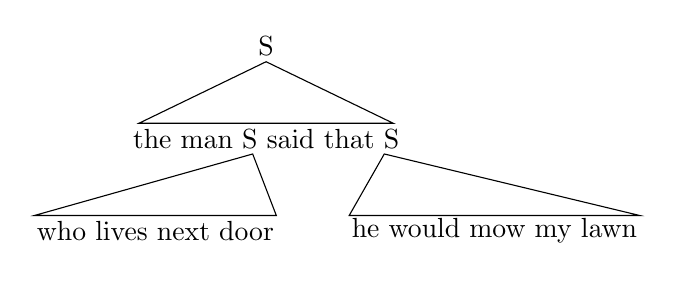
\begin{tikzpicture}
\node at (3.075275,0.) {S};
\draw (3.075275,-.195255) -- (1.46143202017483,-.976275) -- (4.68911797982517,-.976275) -- cycle;
\node at (3.075275,-1.17153) {the~man~S~said~that~S};
\draw (2.90498111460882,-1.366785) -- (.133972614177315,-2.147805) -- (3.20489738582268,-2.147805) -- cycle;
\draw (4.57634069730695,-1.366785) -- (4.13091142067728,-2.147805) -- (7.81872857932272,-2.147805) -- cycle;
\node at (1.669435,-2.34306) {who~lives~next~door};
\node at (5.97482,-2.34306) {he~would~mow~my~lawn};
\end{tikzpicture}
\end{minipage}
\bigbreak

\bigbreak
\begin{minipage}{\textwidth}
\begin{enumerate*}
\item[(1.52)] Somebody seduced Bill's sister, but no one will
ever seduce Jack's and she knows it.
\end{enumerate*}
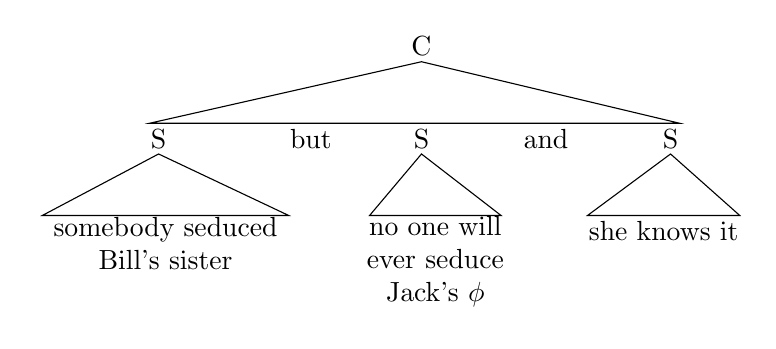
\begin{tikzpicture}
\node at (4.656845,0.) {C};
\draw (4.656845,-.195255) -- (1.20519771748179,-.976275) -- (7.93276228251821,-.976275) -- cycle;
\node at (1.317975,-1.17153) {S};
\node at (3.251005,-1.17153) {but};
\node at (4.656845,-1.17153) {S};
\node at (6.238415,-1.17153) {and};
\node at (7.819985,-1.17153) {S};
\draw (1.317975,-1.366785) -- (-.158379570766975,-2.147805) -- (2.97005957076698,-2.147805) -- cycle;
\draw (4.656845,-1.366785) -- (3.9980230687655,-2.147805) -- (5.6671269312345,-2.147805) -- cycle;
\draw (7.819985,-1.366785) -- (6.76561939728396,-2.147805) -- (8.69862060271604,-2.147805) -- cycle;
\node at (1.40584,-2.538315) {\begin{tabular}{cc}
                                somebody~seduced\\
                                Bill's~sister
                              \end{tabular}};
\node at (4.832575,-2.73357) {\begin{tabular}{cc}
                               no~one~will\\
                               ever~seduce\\
                               Jack's~${\phi}$
                             \end{tabular}};
\node at (7.73212,-2.34306) {she~knows~it};
\end{tikzpicture}
\end{minipage}
\bigbreak

%%%%%%%%%%%%%%%%%%%%%%%%%%%%%%%%%%%%%%%%%%%%%%%%%%%%%%%%%%%%%%%%

\subsection{Clauses}

\index{clause!adverbial}
\textbf{Adverbial clauses} are clauses beginning with an adverb.
Some examples are (1.53)-(1.57) below.

\begin{enumerate*}
\item[(1.53)] after Fido made a mess on the carpet
\item[(1.54)] before George kisses Betty
\item[(1.55)] since John is an asshole
\item[(1.56)] until Cathy behaves herself
\item[(1.57)] although Lile flunked all his classes
\end{enumerate*}

\index{clause!that}
Clauses complemented with \underline{that} are \textbf{that clauses}.
Example (1.58) is a that clause.

\begin{enumerate*}
\item[(1.58)] that Snoopy is a cat
\end{enumerate*}

\index{clause!infinitive}
\index{transformation!For-To}
Clauses modified by the \textbf{For-To Transformation} are
\textbf{infinitive clauses}. Example (1.59) is an infinitive
clause.

\begin{enumerate*}
\item[(1.59)] for Ruth to choose
\end{enumerate*}

\index{clause!genitive}
\index{transformation!Possessive-Ing}
Clauses modified by the \textbf{Possessive-Ing Transformation}
are \textbf{genitive clauses}. Example (1.60) is a genitive
clause.

\begin{enumerate*}
\item[(1.60)] Mary's kissing Bob
\end{enumerate*}

\index{clause!relative}
\index{transformation!WH-Fronting}
\index{transformation!Question}
Clauses modified by \textbf{WH-Fronting Transformation} but not
the \textbf{Question Transformation} and which modify noun
phrases are \textbf{relative clauses}. Examples (1.61)-(1.65)
are relative clauses.

\begin{enumerate*}
\item[(1.61)] who ate five hamburgers
\item[(1.62)] that has a leaky faucet
\item[(1.63)] which doesn't run
\item[(1.64)] whom he gave it to
\item[(1.65)] whose life isn't worth a postage stamp
\end{enumerate*}

\index{clause}
\index{clause!subordinate}
\index{clause!simplex}
\index{simplex|see {clause, simplex}}
\textbf{Clauses} without embedded \textbf{subordinate clauses}
are \textbf{simplex}. In example (1.66) from
Ross\cite{Ross67}, the simplexes are (1.67)-(1.69). In example
(1.70), from Huddleston~\cite{Huddleston78}, the simplexes are
(1.71)-(1.73). In example (1.74), from Huddleston, the simplexes
are (1.75)-(1.77).

\bigbreak
\begin{minipage}{\textwidth}
\begin{enumerate*}
\item[(1.66)] Realizing that he was unpopular didn't disturb
Oscar.
\end{enumerate*}
\bigbreak
\centering
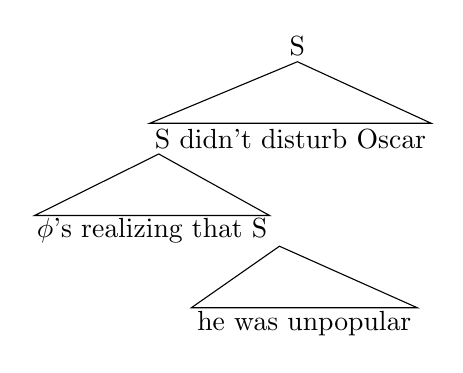
\begin{tikzpicture}
\node at (3.778195,0.) {S};
\draw (3.778195,-.195255) -- (1.90506628966198,-.976275) -- (5.47559371033802,-.976275) -- cycle;
\node at (3.69033,-1.17153) {S~didn't~disturb~Oscar};
\draw (2.01784357218019,-1.366785) -- (0.442215532527226,-2.147805) -- (3.42384446747277,-2.147805) -- cycle;
\node at (1.93303,-2.34306) {${\phi}$'s~realizing~that~S};
\draw (3.55025574817456,-2.538315) -- (2.43209731054271,-3.319335) -- (5.30002268945729,-3.319335) -- cycle;
\node at (3.86606,-3.51459) {he~was~unpopular};
\end{tikzpicture}
\bigbreak
\vbox{\obeylines{
${\phi}$ \textit{precedes} he
${\phi}$ \textit{commands} he
${\phi}$ \textit{precedes} Oscar
Oscar \textit{commands} ${\phi}$
Oscar \textit{commands} he
}}
\end{minipage}
\bigbreak

\begin{enumerate*}
\item[(1.67)] S didn't disturb Oscar
\item[(1.68)] ${\phi}$'s realizing that S
\item[(1.69)] he was unpopular
\end{enumerate*}

\bigbreak
\begin{minipage}{\textwidth}
\begin{enumerate*}
\item[(1.70)] My neighbor who is pregnant said that she was
very happy.
\end{enumerate*}
\bigbreak
\centering
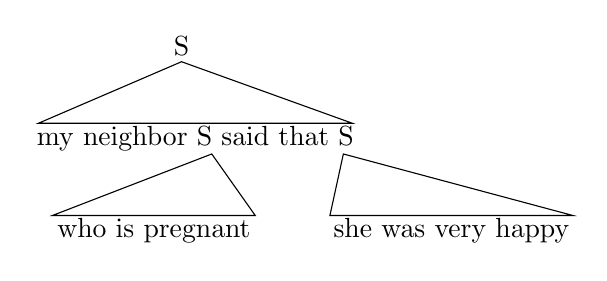
\begin{tikzpicture}
\node at (2.020895,0.) {S};
\draw (2.020895,-.195255) -- (.204413980533021,-.976275) -- (4.18883601946698,-.976275) -- cycle;
\node at (2.196625,-1.17153) {my~neighbor~S~said~that~S};
\draw (2.40469915425063,-1.366785) -- (.382082757516534,-2.147805) -- (2.95678724248347,-2.147805) -- cycle;
\draw (4.07605873694877,-1.366785) -- (3.90540146848279,-2.147805) -- (6.98985853151721,-2.147805) -- cycle;
\node at (1.669435,-2.34306) {who~is~pregnant};
\node at (5.44763,-2.34306) {she~was~very~happy};
\end{tikzpicture}
\bigbreak
\vbox{\obeylines{
neighbor \textit{precedes} she
neighbor \textit{commands} she
}}
\end{minipage}
\bigbreak

\begin{enumerate*}
\item[(1.71)] my neighbor said that S
\item[(1.72)] who is pregnant
\item[(1.73)] she was very happy
\end{enumerate*}

\bigbreak
\begin{minipage}{\textwidth}
\begin{enumerate*}
\item[(1.74)] The pilot who shot at it hit the Mig that chased
him.
\end{enumerate*}
\bigbreak
\centering
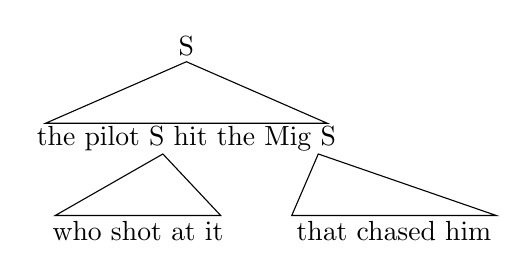
\begin{tikzpicture}
\node at (2.196625,0.) {S};
\draw (2.196625,-.195255) -- (.409104960437095,-.976275) -- (3.9841450395629,-.976275) -- cycle;
\node at (2.196625,-1.17153) {the~pilot~S~hit~the~Mig~S};
\draw (1.89776521147666,-1.366785) -- (.5316134327659,-2.147805) -- (2.6315265672341,-2.147805) -- cycle;
\draw (3.87136775704469,-1.366785) -- (3.53450889842242,-2.147805) -- (6.13064110157758,-2.147805) -- cycle;
\node at (1.58157,-2.34306) {who~shot~at~it};
\node at (4.832575,-2.34306) {that~chased~him};
\end{tikzpicture}
\bigbreak
\vbox{\obeylines{
pilot \textit{precedes} him
pilot \textit{commands} him
it \textit{precedes} the Mig
Mig \textit{commands} it
}}
\end{minipage}
\bigbreak

\begin{enumerate*}
\item[(1.75)] the pilot hit the Mig
\item[(1.76)] who shot at it
\item[(1.77)] that chased him
\end{enumerate*}

%%%%%%%%%%%%%%%%%%%%%%%%%%%%%%%%%%%%%%%%%%%%%%%%%%%%%%%%%%%%%%%%

\subsection{Precedes and Commands}

\index{relation!precedes@\textit{precedes}}
\index{relation!commands@\textit{commands}}
The \textbf{\textit{precedes}} and \textbf{\textit{commands}}
relations, first described by Langacker~\cite{Langacker69},
are defined below in (1.78) and (1.79).

\index{relation!dominates@\textit{dominates}}
\begin{enumerate*}
\item[(1.78)] \textbf{\textit{precedes} Relation}\\
A node A \textit{precedes} another node B if
    \begin{enumerate*}
    \item[(a)] neither A nor B \textbf{\textit{dominates}} the other, and
    \item[(b)] A occurs before B (in preorder traversal)
    \end{enumerate*}
\end{enumerate*}

\begin{enumerate*}
\item[(1.79)] \textbf{\textit{commands} Relation}\\
A node A \textit{commands} another node B if
    \begin{enumerate*}
    \item[(a)] neither A nor B \textit{dominates} the other, and
    \item[(b)] the S-node that most immediately \textit{dominates} 
    A also \textit{dominates} B
    \end{enumerate*}
\end{enumerate*}

\index{relation!is separate from@\textit{is separate from}}
Another relation that will be useful is the
\textbf{\textit{is separate from}} relation defined below in
(1.80).

\begin{enumerate*}
\item[(1.80)] \textbf{\textit{is separate from} Relation}\\
A node R \textit{is separate from} another node B if
    \begin{enumerate*}
    \item[(a)] neither A nor B \textit{dominates} the other, and
    \item[(b)] the lowest node in the tree dominating A
    and B is a C-node.
    \end{enumerate*}
\end{enumerate*}

We will see that \textit{precedes}, \textit{commands}, and
\textit{is separate from} are useful in determining when
pronominalization is or isn't possible.

In example (1.81), A \textit{precedes} B, A \textit{commands} B,
and E \textit{commands} A. We don't have A \textit{precedes} A,
B \textit{precedes} A, B \textit{precedes} B,
A \textit{commands} A, or B \textit{commands} B.

\bigbreak
\begin{minipage}{\textwidth}
\begin{enumerate*}
\item[(1.81)]
\end{enumerate*}
\bigbreak
\centering
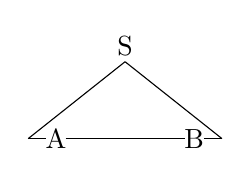
\begin{tikzpicture}
\node at (1.317975,0.) {S};
\draw (1.317975,-.195255) -- (.087865,-1.17153);
\draw (.087865,-1.17153) -- (.316314,-1.17153);
\draw (.562336,-1.17153) -- (2.073614,-1.17153);
\draw (2.319636,-1.17153) -- (2.548085,-1.17153);
\draw (2.548085,-1.17153) -- (1.317975,-.195255);
\node at (.439325,-1.17153) {A};
\node at (2.196625,-1.17153) {B};
\end{tikzpicture}
\bigbreak
\vbox{\obeylines{
A \textit{precedes} B
A \textit{commands} B
B \textit{commands} A
}}
\end{minipage}
\bigbreak

In (1.82), A \textit{precedes} B, A \textit{is separate from} B,
and B \textit{is separate from} A. In (1.83),
A \textit{precedes} B and A \textit{commands} B.  In (1.84),
A \textit{precedes} B and B \textit{commands} A. In (1.85),
A \textit{precedes} B, H \textit{is separate from} B, and
B \textit{is separate from} A.

\bigbreak
\begin{minipage}{\textwidth}
\begin{enumerate*}
\item[(1.82)]
\end{enumerate*}
\bigbreak
\centering
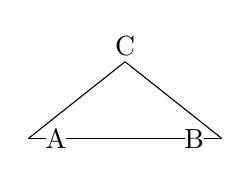
\begin{tikzpicture}
\node at (1.317975,0.) {C};
\draw (1.317975,-.195255) -- (.087865,-1.17153);
\draw (.087865,-1.17153) -- (.316314,-1.17153);
\draw (.562336,-1.17153) -- (2.073614,-1.17153);
\draw (2.319636,-1.17153) -- (2.548085,-1.17153);
\draw (2.548085,-1.17153) -- (1.317975,-.195255);
\node at (.439325,-1.17153) {A};
\node at (2.196625,-1.17153) {B};
\end{tikzpicture}
\bigbreak
\vbox{\obeylines{
A \textit{precedes} B
A \textit{is separate from} B
A \textit{precedes} B
}}
\end{minipage}
\bigbreak

\bigbreak
\begin{minipage}{\textwidth}
\begin{enumerate*}
\item[(1.83)]
\end{enumerate*}
\bigbreak
\centering
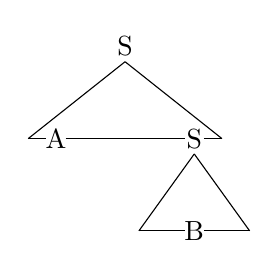
\begin{tikzpicture}
\node at (1.317975,0.) {S};
\draw (1.317975,-.195255) -- (.087865,-1.17153);
\draw (.087865,-1.17153) -- (.316314,-1.17153);
\draw (.562336,-1.17153) -- (2.073614,-1.17153);
\draw (2.319636,-1.17153) -- (2.548085,-1.17153);
\draw (2.548085,-1.17153) -- (1.317975,-.195255);
\node at (.439325,-1.17153) {A};
\node at (2.196625,-1.17153) {S};
\draw (2.196625,-1.366785) -- (1.493705,-2.34306);
\draw (1.493705,-2.34306) -- (2.073614,-2.34306);
\draw (2.319636,-2.34306) -- (2.899545,-2.34306);
\draw (2.899545,-2.34306) -- (2.196625,-1.366785);
\node at (2.196625,-2.34306) {B};
\end{tikzpicture}
\bigbreak
\vbox{\obeylines{
A \textit{precedes} B
A \textit{commands} B
}}
\end{minipage}
\bigbreak

\bigbreak
\begin{minipage}{\textwidth}
\begin{enumerate*}
\item[(1.84)]
\end{enumerate*}
\bigbreak
\centering
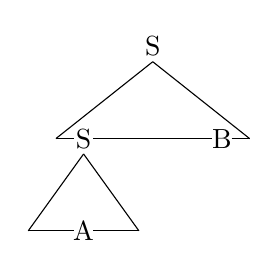
\begin{tikzpicture}
\node at (1.669435,0.) {S};
\draw (1.669435,-.195255) -- (.439325,-1.17153);
\draw (.439325,-1.17153) -- (.667774,-1.17153);
\draw (.913796,-1.17153) -- (2.425074,-1.17153);
\draw (2.671096,-1.17153) -- (2.899545,-1.17153);
\draw (2.899545,-1.17153) -- (1.669435,-.195255);
\node at (.790785,-1.17153) {S};
\node at (2.548085,-1.17153) {B};
\draw (.790785,-1.366785) -- (.087865,-2.34306);
\draw (.087865,-2.34306) -- (.667774,-2.34306);
\draw (.913796,-2.34306) -- (1.493705,-2.34306);
\draw (1.493705,-2.34306) -- (.790785,-1.366785);
\node at (.790785,-2.34306) {A};
\end{tikzpicture}
\bigbreak
\vbox{\obeylines{
A \textit{precedes} B
B \textit{commands} A
}}
\end{minipage}
\bigbreak

\bigbreak
\begin{minipage}{\textwidth}
\begin{enumerate*}
\item[(1.85)]
\end{enumerate*}
\bigbreak
\centering
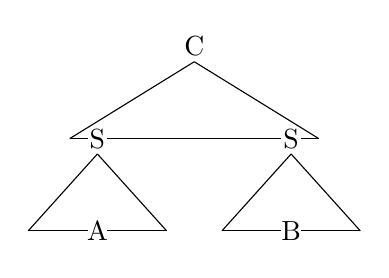
\begin{tikzpicture}
\node at (2.196625,0.) {C};
\draw (2.196625,-.195255) -- (.615055,-1.17153);
\draw (.615055,-1.17153) -- (.843504,-1.17153);
\draw (1.089526,-1.17153) -- (3.303724,-1.17153);
\draw (3.549746,-1.17153) -- (3.778195,-1.17153);
\draw (3.778195,-1.17153) -- (2.196625,-.195255);
\node at (.966515,-1.17153) {S};
\node at (3.426735,-1.17153) {S};
\draw (.966515,-1.366785) -- (.087865,-2.34306);
\draw (.087865,-2.34306) -- (.843504,-2.34306);
\draw (1.089526,-2.34306) -- (1.845165,-2.34306);
\draw (1.845165,-2.34306) -- (.966515,-1.366785);
\draw (3.426735,-1.366785) -- (2.548085,-2.34306);
\draw (2.548085,-2.34306) -- (3.303724,-2.34306);
\draw (3.549746,-2.34306) -- (4.305385,-2.34306);
\draw (4.305385,-2.34306) -- (3.426735,-1.366785);
\node at (.966515,-2.34306) {A};
\node at (3.426735,-2.34306) {B};
\end{tikzpicture}
\bigbreak
\vbox{\obeylines{
A \textit{precedes} B
A \textit{is separate from} B
B \textit{is separate from} A
}}
\end{minipage}
\bigbreak

Examples (1.86)-(1.89) are from Langacker~\cite{Langacker69}.

\bigbreak
\begin{minipage}{\textwidth}
\begin{enumerate*}
\item[(1.86)] The mosquito which bit Algernon was killed by
him. [him ${=}$ Algernon]
\end{enumerate*}
\bigbreak
\centering
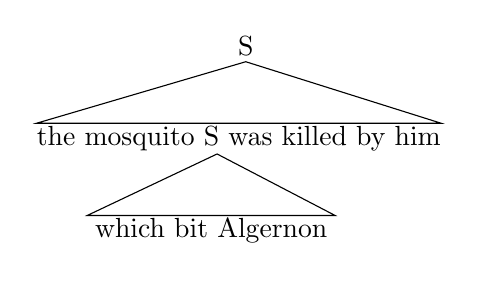
\begin{tikzpicture}
\node at (2.899545,0.) {S};
\draw (2.899545,-.195255) -- (.243741254730433,-.976275) -- (5.37961874526957,-.976275) -- cycle;
\node at (2.81168,-1.17153) {the~mosquito~S~was~killed~by~him};
\draw (2.53537538378229,-1.366785) -- (.886413415260583,-2.147805) -- (4.03402658473942,-2.147805) -- cycle;
\node at (2.46022,-2.34306) {which~bit~Algernon};
\end{tikzpicture}
\bigbreak
\vbox{\obeylines{
Algernon \textit{precedes} him
him \textit{precedes} Algernon
}}
\end{minipage}
\bigbreak

\bigbreak
\begin{minipage}{\textwidth}
\begin{enumerate*}
\item[(1.87)] The mosquito which bit him was killed by
Algernon. [him ${=}$ Algernon]
\end{enumerate*}
\bigbreak
\centering
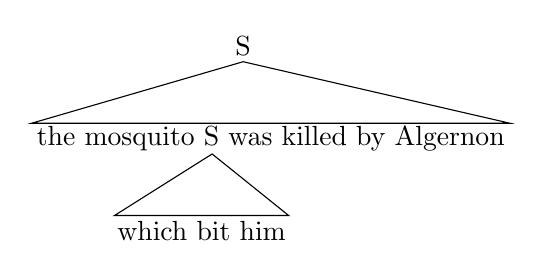
\begin{tikzpicture}
\node at (2.899545,0.) {S};
\draw (2.899545,-.195255) -- (.214476916870361,-.976275) -- (6.28753308312964,-.976275) -- cycle;
\node at (3.251005,-1.17153) {the~mosquito~S~was~killed~by~Algernon};
\draw (2.50611104592222,-1.366785) -- (1.26713775312066,-2.147805) -- (3.47757224687934,-2.147805) -- cycle;
\node at (2.372355,-2.34306) {which~bit~him};
\end{tikzpicture}
\bigbreak
\vbox{\obeylines{
him \textit{precedes} Algernon
Algernon \textit{precedes} him
}}
\end{minipage}
\bigbreak

\bigbreak
\begin{minipage}{\textwidth}
\begin{enumerate*}
\item[(1.88)] Algernon killed the mosquito which bit him.
[him ${=}$ Algernon]
\end{enumerate*}
\bigbreak
\centering
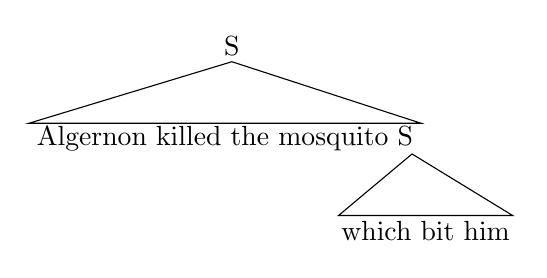
\begin{tikzpicture}
\node at (2.723815,0.) {S};
\draw (2.723815,-.195255) -- (.147519302850326,-.976275) -- (5.12438069714967,-.976275) -- cycle;
\node at (2.63595,-1.17153) {Algernon~killed~the~mosquito~S};
\draw (5.01160341463146,-1.366785) -- (4.07881775312066,-2.147805) -- (6.28925224687934,-2.147805) -- cycle;
\node at (5.184035,-2.34306) {which~bit~him};
\end{tikzpicture}
\bigbreak
\vbox{\obeylines{
Algernon \textit{precedes} him
him \textit{commands} Algernon
}}
\end{minipage}
\bigbreak

\bigbreak
\begin{minipage}{\textwidth}
\begin{enumerate*}
\item[(1.89)] He killed the mosquito which bit Algernon.
[he ${\ne}$ Algernon]
\end{enumerate*}
\bigbreak
\centering
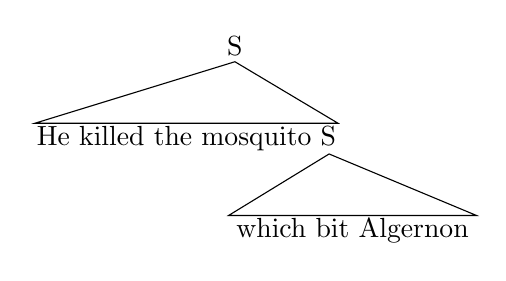
\begin{tikzpicture}
\node at (2.723815,0.) {S};
\draw (2.723815,-.195255) -- (.184779848497261,-.976275) -- (4.03274015150274,-.976275) -- cycle;
\node at (2.10876,-1.17153) {He~killed~the~mosquito~S};
\draw (3.91996286898453,-1.366785) -- (2.64371341526058,-2.147805) -- (5.79132658473942,-2.147805) -- cycle;
\node at (4.21752,-2.34306) {which~bit~Algernon};
\end{tikzpicture}
\bigbreak
\vbox{\obeylines{
he \textit{precedes} Algernon
Algernon \textit{commands} he
}}
\end{minipage}
\bigbreak

\index{Precedes and Commands Rule}
The Precedes and Commands Rule, essentially as stated by
Langacker~\cite{Langacker69}, is given in (1.90) below.

\begin{enumerate*}
\item[(1.90)] \textbf{Precedes and Commands Rule}\\
A pronoun P may be used to pronominalize a noun
phrase NP unless
    \begin{enumerate*}
    \item[(a)] P \textit{precedes} NP, and
    \item[(b)] P \textit{commands} NP or P \textit{is separate from} NP
    \end{enumerate*}
\end{enumerate*}

Note that the Precedes and Commands Rule explains the
grammaticality and ungrammaticality of (1.86)-(1.89). These
further examples from Ross~\cite{Ross67} should drive the
point home.

\begin{enumerate*}
\item[(1.91)] After John Adams woke up, he was hungry.
[he ${=}$ John Adams]
\item[(1.92)] That Oscar was unpopular didn't disturb him.
[him ${=}$ Oscar]
\item[(1.93)] For your brother to refuse to pay taxes would
get him into trouble. [him ${=}$ your brother]
\item[(1.94)] Anna's complaining about Peter infuriated him.
[him ${=}$ Peter]
\item[(1.95)] The possibility that Fred will be unpopular
doesn't bother him. [him ${=}$ Fred]
\end{enumerate*}

\bigbreak
\begin{minipage}{\textwidth}
\centering
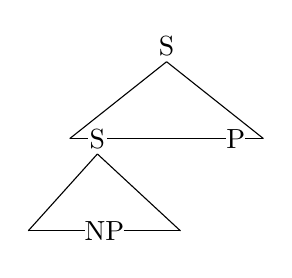
\begin{tikzpicture}
\node at (1.845165,0.) {S};
\draw (1.845165,-.195255) -- (.615055,-1.17153);
\draw (.615055,-1.17153) -- (.843504,-1.17153);
\draw (1.089526,-1.17153) -- (2.600804,-1.17153);
\draw (2.846826,-1.17153) -- (3.075275,-1.17153);
\draw (3.075275,-1.17153) -- (1.845165,-.195255);
\node at (.966515,-1.17153) {S};
\node at (2.723815,-1.17153) {P};
\draw (.966515,-1.366785) -- (.087865,-2.34306);
\draw (.087865,-2.34306) -- (.808358,-2.34306);
\draw (1.300402,-2.34306) -- (2.020895,-2.34306);
\draw (2.020895,-2.34306) -- (.966515,-1.366785);
\node at (1.05438,-2.34306) {NP};
\end{tikzpicture}
\bigbreak
\vbox{\obeylines{
NP \textit{precedes} P
P \textit{commands} NP
}}
\end{minipage}
\bigbreak

\begin{enumerate*}
\item[(1.96)] After he woke up, John Adams was hungry.
[he ${=}$ John Adams]
\item[(1.97)] That he was unpopular didn't disturb Oscar.
[he ${=}$ Oscar]
\item[(1.98)] For him to refuse to pay taxes would get your
brother into trouble. [him ${=}$ your brother]
\item[(1.99)] Anna's complaining about him infuriated Peter.
[him ${=}$ Peter]
\item[(1.100)] The possibility that he will be unpopular
doesn't bother Fred. [him ${=}$ Fred]
\end{enumerate*}

\bigbreak
\begin{minipage}{\textwidth}
\centering
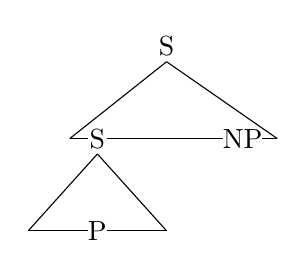
\begin{tikzpicture}
\node at (1.845165,0.) {S};
\draw (1.845165,-.195255) -- (.615055,-1.17153);
\draw (.615055,-1.17153) -- (.843504,-1.17153);
\draw (1.089526,-1.17153) -- (2.565658,-1.17153);
\draw (3.057702,-1.17153) -- (3.251005,-1.17153);
\draw (3.251005,-1.17153) -- (1.845165,-.195255);
\node at (.966515,-1.17153) {S};
\node at (2.81168,-1.17153) {NP};
\draw (.966515,-1.366785) -- (.087865,-2.34306);
\draw (.087865,-2.34306) -- (.843504,-2.34306);
\draw (1.089526,-2.34306) -- (1.845165,-2.34306);
\draw (1.845165,-2.34306) -- (.966515,-1.366785);
\node at (.966515,-2.34306) {P};
\end{tikzpicture}
\bigbreak
\vbox{\obeylines{
P \textit{precedes} NP
NP \textit{commands} P
}}
\end{minipage}
\bigbreak

\begin{enumerate*}
\item[(1.101)] John Adams was hungry after he woke up.
[he ${=}$ John Adams]
\item[(1.102)] Oscar wasn't disturbed that he was unpopular.
[he ${=}$ Oscar]
\item[(1.103)] It would get your brother into trouble for him
to refuse to pay taxes. [him ${=}$ your brother]
\item[(1.104)] Peter was infuriated at Anna's complaining
about him. [him ${=}$ Peter]
\item[(1.105)] Fred isn't bothered by the possibility that he
will be unpopular. [he ${=}$ Fred]
\end{enumerate*}

\bigbreak
\begin{minipage}{\textwidth}
\centering
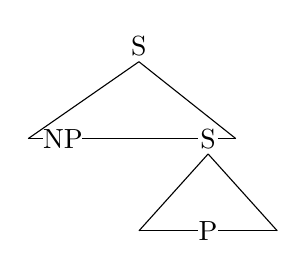
\begin{tikzpicture}
\node at (1.493705,0.) {S};
\draw (1.493705,-.195255) -- (.087865,-1.17153);
\draw (.087865,-1.17153) -- (.281168,-1.17153);
\draw (.773212,-1.17153) -- (2.249344,-1.17153);
\draw (2.495366,-1.17153) -- (2.723815,-1.17153);
\draw (2.723815,-1.17153) -- (1.493705,-.195255);
\node at (.52719,-1.17153) {NP};
\node at (2.372355,-1.17153) {S};
\draw (2.372355,-1.366785) -- (1.493705,-2.34306);
\draw (1.493705,-2.34306) -- (2.249344,-2.34306);
\draw (2.495366,-2.34306) -- (3.251005,-2.34306);
\draw (3.251005,-2.34306) -- (2.372355,-1.366785);
\node at (2.372355,-2.34306) {P};
\end{tikzpicture}
\bigbreak
\vbox{\obeylines{
NP \textit{precedes} P
NP \textit{commands} P
}}
\end{minipage}
\bigbreak

\begin{enumerate*}
\item[(1.106)] *He was hungry after John Adams woke up.
[he ${=}$ John Adams]
\item[(1.107)] *He wasn't disturbed that Oscar was unpopular.
[he ${=}$ Oscar]
\item[(1.108)] *It would get him into trouble for your brother
to refuse to pay taxes. [him ${=}$ your brother]
\item[(1.109)] *He was infuriated at Anna's complaining about
Peter. [he ${=}$ Peter]
\item[(1.110)] *He isn't bothered by the possibility that Fred
will be unpopular. [he ${=}$ Fred]
\end{enumerate*}

\bigbreak
\begin{minipage}{\textwidth}
\centering
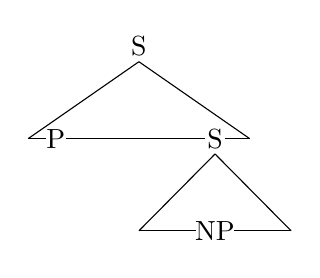
\begin{tikzpicture}
\node at (1.493705,0.) {S};
\draw (1.493705,-.195255) -- (.087865,-1.17153);
\draw (.087865,-1.17153) -- (.316314,-1.17153);
\draw (.562336,-1.17153) -- (2.337209,-1.17153);
\draw (2.583231,-1.17153) -- (2.899545,-1.17153);
\draw (2.899545,-1.17153) -- (1.493705,-.195255);
\node at (.439325,-1.17153) {P};
\node at (2.46022,-1.17153) {S};
\draw (2.46022,-1.366785) -- (1.493705,-2.34306);
\draw (1.493705,-2.34306) -- (2.214198,-2.34306);
\draw (2.706242,-2.34306) -- (3.426735,-2.34306);
\draw (3.426735,-2.34306) -- (2.46022,-1.366785);
\node at (2.46022,-2.34306) {NP};
\end{tikzpicture}
\bigbreak
\vbox{\obeylines{
P \textit{precedes} NP
P \textit{commands} NP
}}
\end{minipage}
\bigbreak

\bigbreak
\index{sentence!conjoined}
Examples (1.111) and (1.112) from Langacker~\cite{Langacker69}
illustrate the Precedes and Commands Rule for
\textbf{conjoined structures}.

\bigbreak
\begin{minipage}{\textwidth}
\begin{enumerate*}
\item[(1.111)] Penelope cursed Peter and slandered him.
[him ${=}$ Peter]
\end{enumerate*}
\bigbreak
\centering
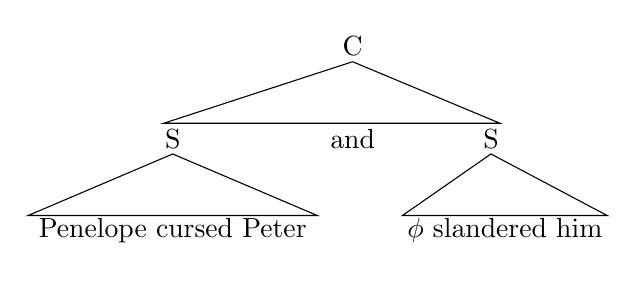
\begin{tikzpicture}
\node at (4.129655,0.) {C};
\draw (4.129655,-.195255) -- (1.73238771748179,-.976275) -- (5.99973228251821,-.976275) -- cycle;
\node at (1.845165,-1.17153) {S};
\node at (4.129655,-1.17153) {and};
\node at (5.886955,-1.17153) {S};
\draw (1.845165,-1.366785) -- (.0102813315796613,-2.147805) -- (3.68004866842034,-2.147805) -- cycle;
\draw (5.886955,-1.366785) -- (4.76359233910521,-2.147805) -- (7.3617776608947905,-2.147805) -- cycle;
\node at (1.845165,-2.34306) {Penelope~cursed~Peter};
\node at (6.062685,-2.34306) {${\phi}$~slandered~him};
\end{tikzpicture}
\bigbreak
\vbox{\obeylines{
Peter \textit{precedes} him
Peter \textit{is separate from} him
him \textit{is separate from} Peter
}}
\end{minipage}
\bigbreak

\bigbreak
\begin{minipage}{\textwidth}
\begin{enumerate*}
\item[(1.112)] *Penelope cursed him and slandered Peter.
[him ${=}$ Peter]
\end{enumerate*}
\bigbreak
\centering
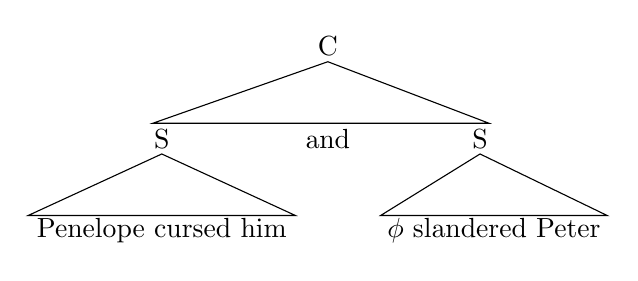
\begin{tikzpicture}
\node at (3.778195,0.) {C};
\draw (3.778195,-.195255) -- (1.55665771748179,-.976275) -- (5.82400228251821,-.976275) -- cycle;
\node at (1.669435,-1.17153) {S};
\node at (3.778195,-1.17153) {and};
\node at (5.711225,-1.17153) {S};
\draw (1.669435,-1.366785) -- (-.0267336482456835,-2.147805) -- (3.36560364824568,-2.147805) -- cycle;
\draw (5.711225,-1.366785) -- (4.4491473189305495,-2.147805) -- (7.32476268106945,-2.147805) -- cycle;
\node at (1.669435,-2.34306) {Penelope~cursed~him};
\node at (5.886955,-2.34306) {${\phi}$~slandered~Peter};
\end{tikzpicture}
\bigbreak
\vbox{\obeylines{
him \textit{precedes} Peter
him \textit{is separate from} Peter
Peter \textit{is separate from} him
}}
\end{minipage}
\bigbreak

\bigbreak
Examples (1.113) and (1.114) adapted from Chiba~\cite{Chiba71}
involve
\index{deletion!Equi-NP}
Equi-NP Deletion.

\bigbreak
\begin{minipage}{\textwidth}
\begin{enumerate*}
\item[(1.113)] The interest in visiting Las Vegas that Mary
displayed is typical of gamblers.
\end{enumerate*}
\bigbreak
\centering
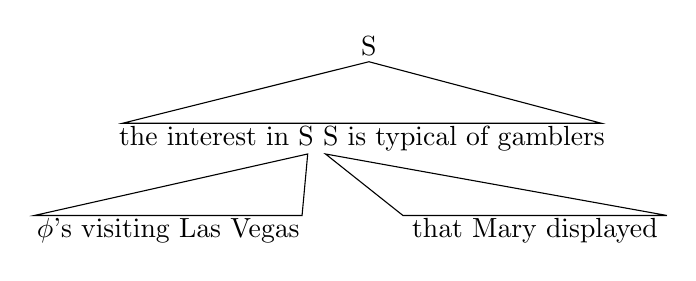
\begin{tikzpicture}
\node at (4.656845,0.) {S};
\draw (4.656845,-.195255) -- (1.53076114169141,-.976275) -- (7.60719885830859,-.976275) -- cycle;
\node at (4.56898,-1.17153) {the~interest~in~S~S~is~typical~of~gamblers};
\draw (3.87990964063185,-1.366785) -- (0.409307448219311,-2.147805) -- (3.8082125517806897,-2.147805) -- cycle;
\draw (4.10546420566827,-1.366785) -- (5.08917045278345,-2.147805) -- (8.44203954721655,-2.147805) -- cycle;
\node at (2.10876,-2.34306) {${\phi}$'s~visiting~Las~Vegas};
\node at (6.765605,-2.34306) {that~Mary~displayed};
\end{tikzpicture}
\bigbreak
\vbox{\obeylines{
${\phi}$ \textit{precedes} Mary
}}
\end{minipage}
\bigbreak

%%%%%%%%%%%%%%%%%%%%%%%%%%%%%%%%%%%%%%%%%%%%%%%%%%%%%%%%%%%%%%%%
%
%     Resolution Module
%
%%%%%%%%%%%%%%%%%%%%%%%%%%%%%%%%%%%%%%%%%%%%%%%%%%%%%%%%%%%%%%%%

\section{Resolution Module}
\index{Resolution}
\index{Pronoun Resolution|see {Resolution}}

%%%%%%%%%%%%%%%%%%%%%%%%%%%%%%%%%%%%%%%%%%%%%%%%%%%%%%%%%%%%%%%%

\subsection{Introduction}

In the previous chapter we touched upon some basic notions such
as the \textit{precedes}, \textit{commands}, and
\textit{is separate from} relations. We will see in the coming
chapters how these concepts give rise to a very promising
approach to the problem of pronoun resolution.

The algorithm we shall describe won't be complete in the sense
that we will elaborate and refine it in later chapters and after
we are done it will need elaboration and refinement, but it will
be set in firm soil so that we have a foundation on which to
build. Because personal and reflexive pronouns are easiest,
these are the pronouns we shall consider first. But before we go
any farther, let us take time out to indicate something of the
environment and structure of the module that does resolving of
pronouns in a natural language system, the Resolution module.

%%%%%%%%%%%%%%%%%%%%%%%%%%%%%%%%%%%%%%%%%%%%%%%%%%%%%%%%%%%%%%%%

\subsection{Environment}
\index{Environment}

The center of a natural language system is the Language
Processor module which is divided into five submodules.  These
are the Language Driver, Preprocesor, Parser, Semantic
Processor, and Output Processor as indicated in Figure~2.1.

\bigbreak
\begin{figure}[htp]
\centering
\begin{tikzpicture}[
    box/.style={draw, rectangle, minimum width=1.875cm, minimum height=.75cm, text centered, font=\sffamily},
    connect/.style={draw, thick, -latex}
    ]
% Nodes
\node[box] (driver) {\begin{tabular}{cc}
    Language\\Driver
  \end{tabular}};
\matrix[row sep=1.5cm, column sep=.375cm, below=of driver] (m) {
  \node[box] (preprocessor) {\begin{tabular}{cc}
    Preprocessor
  \end{tabular}}; & 
  \node[box] (parser) {\begin{tabular}{cc}
    Parser
  \end{tabular}}; &
  \node[box] (semantic) {\begin{tabular}{cc}
    Semantic\\Processor
  \end{tabular}}; &
  \node[box] (output) {\begin{tabular}{cc}
    Output\\Processor
  \end{tabular}}; \\
};
% Connections
\draw[connect] (driver.south) to[out=225,in=90] (preprocessor.north);
\draw[connect] (driver.south) to[out=255,in=90] (parser.north);
\draw[connect] (driver.south) to[out=285,in=90] (semantic.north);
\draw[connect] (driver.south) to[out=315,in=90] (output.north);
\end{tikzpicture}
\end{figure}
\index{Language Driver}
\index{Preprocessor}
\index{Parser}
\index{Semantic Processor}
\index{Output Processor}
\bigbreak
\textbf{Figure~2.1. Submodules of the Language Processor}
\bigbreak

\index{Operating System}
Briefly, from the point of view of the Language Processor, the
following happens. A user types input at a terminal which is
picked up by the Operating System of the natural language
system. The Operating System maintains information about the
user including the language version he is in as well as his
state in that version. The user's state is known as his
prefix. The Operating System, after picking up a user's input
calls a Process Input routine of the Language Driver in the
Language Processor. Once in the Language Driver, the first
module to be called upon is the Preprocessor.

\index{Preprocessor}
The Preprocessor in the Language Processor compresses blanks in
the input string, straps right and left delimiters about it,
recognizes and builds parsing graph arcs over identifiers and
numbers, and looks the identifiers up in the lexicon. After
calling the Preprocessor, the
\index{Language Driver}
Language Driver calls the Parser.

\index{Parser}
\index{Kay algorithm}
The Parser in the Language Processor parses the output.  of the
Preprocessor using an algorithm such as the
\textbf{Kay algorithm} and can handle any general rewrite rule
grammar.  Of course, since a sentence may be ambiguous, more
than one system parse tree may be passed back by the Parser. If
no good parsings are found, then the Syntax Diagnostics routine
of the Syntax Diagnostics module of the natural language system
is called. Otherwise, if there are good parsings, then the
Language Driver calls the Semantic Processor on the output of
the Parser.

\index{Semantic Processor}
The Semantic Processor is driven by the syntax of a system parse
tree into making calls on semantic routines which can be
postprocedures (called on their arguments after their arguments
evaluate themselves), preprocedures (called on their arguments
before their arguments evaluate themselves), and syntax
procedures (called at syntax time during parsing before
preprocedures and postprocedures are called during semantic
processing). On return to the Language Driver, the Language
Driver calls the Output Processor on the output of the Semantic
Processor.

\index{Output Processor}
The Output Processor does some relatively menial processing such
as removing duplicate lines from the output line list which will
be sent back to the Operating System.  The Output Processor is
able to handle ambiguous output and removes diagnostic messages
if at least one of the outputs is good.

On completion of the call on the Output Processor, the Language
Driver returns to the Operating System and the Operating System
displays the output line list on the user's terminal, at the
same time updating its information on the user.

From the discussion of the \textit{precedes}, \textit{commands},
and \textit{is separate from} relations in the previous chapter,
we know that information about the syntax of the input sentence
is critical to the resolving of pronouns in the input sentence.
On the other hand, for semantic processing to carry out the
processing it needs to carry out, the placing of information on
the chaining of pronouns must already be placed in the system
parse tree of the input sentence.

The logical conclusion of these two observations indicates that
pronoun resolution takes place after parsing, but before
semantic processing. This relationship of the Resolution module
with the other modules of the Language Processor is indicated in
Figure~2.2.

\goodbreak
\bigbreak
\noindent\begin{tikzpicture}[
    box/.style={draw, rectangle, minimum width=1.875cm, minimum height=.75cm, text centered, font=\sffamily},
    connect/.style={draw, thick, -latex}
    ]
% Nodes
\node[box] (driver) {\begin{tabular}{cc}
    Language\\Driver
  \end{tabular}};
\matrix[row sep=1.5cm, column sep=.375cm, below=of driver] (m) {
  \node[box] (preprocessor) {\begin{tabular}{cc}
    Preprocessor
  \end{tabular}}; & 
  \node[box] (parser) {\begin{tabular}{cc}
    Parser
  \end{tabular}}; &
  \node[box] (pronoun) {\begin{tabular}{cc}
    Pronoun\\Resolution
  \end{tabular}}; &
  \node[box] (semantic) {\begin{tabular}{cc}
    Semantic\\Processor
  \end{tabular}}; &
  \node[box] (output) {\begin{tabular}{cc}
    Output\\Processor
  \end{tabular}}; \\
};
% Connections
\draw[connect] (driver.south) to[out=210,in=90] (preprocessor.north);
\draw[connect] (driver.south) to[out=240,in=90] (parser.north);
\draw[connect] (driver.south) to[out=270,in=90] (pronoun.north);
\draw[connect] (driver.south) to[out=300,in=90] (semantic.north);
\draw[connect] (driver.south) to[out=330,in=90] (output.north);
\end{tikzpicture}
\index{Language Driver}
\index{Preprocessor}
\index{Parser}
\index{Resolution}
\index{Semantic Processor}
\index{Output Processor}
\bigbreak
\textbf{Figure~2.2. Resolution Module within the Language Processor}
\bigbreak

In practice, this formulation may not be quite correct because
there can be other versions than English which will have nothing
to do with the
\index{Resolution}
Pronoun Resolution module and so what we end up doing is making
the Resolution module accessible via a semantic preprocedure
which is associated with the parsing of the right delimiter of a
sentence. So instead, what happens is that the first semantic
preprocedure to be called will be the procedure which handles
Pronoun Resolution.

%%%%%%%%%%%%%%%%%%%%%%%%%%%%%%%%%%%%%%%%%%%%%%%%%%%%%%%%%%%%%%%%

\subsection{Structure inside the Resolution Module}
\index{Resolution}

The Resolution module is partitioned into seven submodules
besides a Global Declarations module. These are the Node
Processor, Parser, Primary Utilities, Secondary Utilities, Table
Processor, Table Interpreter, and
\index{Resolution Driver}
Resolution Driver modules. The reader should not confuse the
Parser of the Language Processor with the Parser of the Pronoun
Resolution module which have entirely different functions. The
relationship of these submodules of the Resolution module is
indicated below in Figure~2.3.

%We hate to \clearpage, but we don't have a better quick solution
%here.  A minipage won't work here.
\clearpage
\bigbreak
\index{Resolution Driver}
\index{Parser}
\index{Table Processor}
\index{Table Interpreter}
\index{Secondary Utilities}
\index{Primary Utilities}
\index{Node Processor}
\begin{figure}[htp]
\centering
\begin{tikzpicture}[
    box/.style={draw, rectangle, minimum width=1.875cm, minimum height=.75cm, text centered, font=\sffamily},
    connect/.style={draw, thick, -latex}
    ]
% Nodes
\node[box] (resolution) {\begin{tabular}{cc}
    Resolution\\Driver
  \end{tabular}};
\node[box, below=of resolution] (table@proc) {\begin{tabular}{cc}
    Table\\Processor
  \end{tabular}};
\node[box, below=of table@proc] (secondary@uty) {\begin{tabular}{cc}
    Secondary\\Utilities
  \end{tabular}};
\node[box, below=of secondary@uty] (primary@uty) {\begin{tabular}{cc}
    Primary\\Utilities
  \end{tabular}};
\node[box, below=of primary@uty] (node@proc) {\begin{tabular}{cc}
    Node\\Processor
  \end{tabular}};
\node[box, left=.75cm of table@proc] (parser) {Parser};
\node[box, right=.75cm of table@proc] (table@interp) {\begin{tabular}{cc}
    Table\\Interpreter
  \end{tabular}};
% Connections
\draw[connect] (resolution.south) -- (table@proc.north);
\draw[connect] (resolution.west) to[out=180,in=90] (parser.north);
\draw[connect] (resolution.east) to[out=0,in=90] (table@interp.north);
\draw[connect] (parser.south) to[out=270,in=180] (node@proc.west);
\draw[connect] (table@interp.south) to[out=270,in=0] (node@proc.east);
\draw[connect] (table@proc.south) -- (secondary@uty.north);
\draw[connect] (secondary@uty.south) -- (primary@uty.north);
\draw[connect] (primary@uty.south) -- (node@proc.north);
\end{tikzpicture}
\end{figure}
\textbf{Figure~2.3. Structure of the Resolution Module}
\bigbreak

Not shown is the Global Declarations module which does not have
any procedures itself, but merely defines data structures. The
Global Declarations submodule is accessible by all other
submodules of the Resolution module.

%%%%%%%%%%%%%%%%%%%%%%%%%%%%%%%%%%%%%%%%%%%%%%%%%%%%%%%%%%%%%%%%
%
%     Global Declarations
%
%%%%%%%%%%%%%%%%%%%%%%%%%%%%%%%%%%%%%%%%%%%%%%%%%%%%%%%%%%%%%%%%

\section{Global Declarations}

\index{Global Declarations}
The Global Declarations module defines the data structures
accessible to other modules within the pronoun resolution
module. The Global Declarations module is shown below in
Figure~3.1.

\bigbreak
\begin{minipage}{\textwidth}
\index{const name@\texttt{const} name!PNF@\texttt{PNF}}
\index{const name@\texttt{const} name!FPF@\texttt{FPF}}
\index{const name@\texttt{const} name!SPF@\texttt{SPF}}
\index{const name@\texttt{const} name!TPF@\texttt{TPF}}
\index{const name@\texttt{const} name!PLF@\texttt{PLF}}
\index{const name@\texttt{const} name!GNF@\texttt{GNF}}
\index{const name@\texttt{const} name!ANF@\texttt{ANF}}
\index{const name@\texttt{const} name!RPF@\texttt{RPF}}
\index{const name@\texttt{const} name!N\symbol{95}FEATURES@\texttt{N\symbol{95}FEATURES}}
\index{array type name@\texttt{array type} name|see {type name, array}}
\index{enumeration type name@\texttt{enumeration type} name|see {type name, enumeration}}
\index{pointer type name@\texttt{pointer type} name|see {type name, pointer}}
\index{record type name@\texttt{record type} name|see {type name, record}}
\index{type name@\texttt{type} name!enumeration@\texttt{enumeration}!NodeId@\texttt{NodeId}}
\index{type name@\texttt{type} name!enumeration@\texttt{enumeration}!Feature@\texttt{Feature}}
\index{type name@\texttt{type} name!array@\texttt{array}!Features@\texttt{Features}}
\index{type name@\texttt{type} name!pointer@\texttt{pointer}!StringPointer@\texttt{StringPointer}}
\index{type name@\texttt{type} name!pointer@\texttt{pointer}!NodePointer@\texttt{NodePointer}}
\index{type name@\texttt{type} name!record@\texttt{record}!Node@\texttt{Node}}
\index{Feature!Feature@\texttt{Feature}|see {type name, record, Feature}}
\index{Node!Node@\texttt{Node}|see {type name, record, Node}}
\index{enumeration value!C\symbol{95}NODE@\texttt{C\symbol{95}NODE}}
\index{enumeration value!S\symbol{95}NODE@\texttt{S\symbol{95}NODE}}
\index{enumeration value!N\symbol{95}NODE@\texttt{N\symbol{95}NODE}}
\index{enumeration value!E\symbol{95}NODE@\texttt{E\symbol{95}NODE}}
\index{enumeration value!PLUS@\texttt{PLUS}}
\index{enumeration value!MINUS@\texttt{MINUS}}
\index{enumeration value!QUESTION@\texttt{QUESTION}}
\index{record field@\texttt{record} field!number@\texttt{number}}
\index{record field@\texttt{record} field!up\symbol{95}link@\texttt{up\symbol{95}link}}
\index{record field@\texttt{record} field!down\symbol{95}link@\texttt{down\symbol{95}link}}
\index{record field@\texttt{record} field!left\symbol{95}link@\texttt{left\symbol{95}link}}
\index{record field@\texttt{record} field!right\symbol{95}link@\texttt{right\symbol{95}link}}
\index{record field@\texttt{record} field!thread\symbol{95}link@\texttt{thread\symbol{95}link}}
\index{record field@\texttt{record} field!np\symbol{95}link@\texttt{np\symbol{95}link}}
\index{record field@\texttt{record} field!chain\symbol{95}link@\texttt{chain\symbol{95}link}}
\index{record field@\texttt{record} field!col\symbol{95}link@\texttt{col\symbol{95}link}}
\index{record field@\texttt{record} field!ftr@\texttt{ftr}}
\index{record field@\texttt{record} field!lit@\texttt{lit}}
\index{record field@\texttt{record} field!end\symbol{95}col\symbol{95}link@\texttt{end\symbol{95}col\symbol{95}link}}
\index{record field@\texttt{record} field!pred\symbol{95}link@\texttt{pred\symbol{95}link}}
\index{record field@\texttt{record} field!succ\symbol{95}link@\texttt{succ\symbol{95}link}}
\index{record field@\texttt{record} field!sub@\texttt{sub}}
\index{record variant@\texttt{record} variant!C\symbol{95}NODE@\texttt{C\symbol{95}NODE}}
\index{record variant@\texttt{record} variant!S\symbol{95}NODE@\texttt{S\symbol{95}NODE}}
\index{record variant@\texttt{record} variant!N\symbol{95}NODE@\texttt{N\symbol{95}NODE}}
\index{record variant@\texttt{record} variant!E\symbol{95}NODE@\texttt{E\symbol{95}NODE}}
\vbox{\obeylines{\texttt{
\symbol{35}globals.py
import~sys
from~typing~import~TextIO
from~enum~import~Enum,~IntEnum
from~typing~import~Optional

class~FeatureIndex(IntEnum):~\symbol{35}Feature~indices.
~~~~PNF~=~0~\symbol{35}Pronoun~Feature
~~~~FPF~=~1~\symbol{35}First~Person~Feature
~~~~SPF~=~2~\symbol{35}Second~Person~Feature
~~~~TPF~=~3~\symbol{35}Third~Person~Feature
~~~~PLF~=~4~\symbol{35}Plural~Feature
~~~~GNF~=~5~\symbol{35}Gender~Feature
~~~~ANF~=~6~\symbol{35}Animate~Feature
~~~~RPF~=~7~\symbol{35}Reflexive~Feature
~~~~GEN~=~8~\symbol{35}Genitive~Feature

N\symbol{95}FEATURES~=~len(FeatureIndex)~\symbol{35}Number~of~Features

class~NodeId(Enum):~\symbol{35}Identifies~the~type~of~node.
~~~~C\symbol{95}NODE~=~0~\symbol{35}Represents~a~C-node.
~~~~S\symbol{95}NODE~=~1~\symbol{35}Represents~an~S-node.
~~~~N\symbol{95}NODE~=~2~\symbol{35}Represents~an~N-node.
~~~~E\symbol{95}NODE~=~3~\symbol{35}Represents~an~E-node.

class~Feature(Enum):~\symbol{35}Linguistic~feature~values.
~~~~PLUS~=~0~\symbol{35}Has~this~feature.
~~~~MINUS~=~1~\symbol{35}Doesn't~have~this~feature.
~~~~QUESTION~=~2~\symbol{35}Might~or~might~not~have~this~feature.

Features~=~list[Feature]~\symbol{35}list~of~Feature~enums
}}}
\bigbreak
\index{module@\texttt{module}!parser@\texttt{globals}}
\index{globals@\texttt{globals}|see {module, globals}}
\textbf{Figure~3.1. Global Declarations Module (Part I)}
\end{minipage}
\bigbreak

\bigbreak
\begin{minipage}{\textwidth}
\vbox{\obeylines{\texttt{
class~Node:~\symbol{35}Base~node~class
~~~~\symbol{35}~Current~tree
~~~~\symbol{95}tree:~Optional['Node']~=~None
~~~~def~\symbol{95}\symbol{95}init\symbol{95}\symbol{95}(self):
~~~~~~~~self.number:~int~=~0
~~~~~~~~self.up\symbol{95}link:~Optional['Node']~=~None
~~~~~~~~self.down\symbol{95}link:~Optional['Node']~=~None
~~~~~~~~self.left\symbol{95}link:~Optional['Node']~=~None
~~~~~~~~self.right\symbol{95}link:~Optional['Node']~=~None
~~~~~~~~self.thread\symbol{95}link:~Optional['Node']~=~None
~~~~~~~~self.np\symbol{95}link:~Optional['Node']~=~None
~~~~~~~~self.chain\symbol{95}link:~Optional['Node']~=~None
~~~~~~~~self.col\symbol{95}link:~Optional['Node']~=~None
~~~~~~~~self.ftr:~Features~=~[Feature.QUESTION]~*~N\symbol{95}FEATURES
~~~~~~~~self.id:~NodeId~=~NodeId.C\symbol{95}NODE
~~~~~~~~self.lit:~str~=~""
~~~~~~~~self.end\symbol{95}col\symbol{95}link:~Optional['Node']~=~None
~~~~~~~~self.pred\symbol{95}link:~Optional['Node']~=~None
~~~~~~~~self.succ\symbol{95}link:~Optional['Node']~=~None
~~~~~~~~self.sub:~str~=~'~'
~~~~@classmethod
~~~~def~tree(cls)~->~Optional['Node']:
~~~~~~~~return~cls.\symbol{95}tree
~~~~@classmethod
~~~~def~set\symbol{95}tree(cls,~new\symbol{95}tree:~'Node')~->~None:
~~~~~~~~cls.\symbol{95}tree~=~new\symbol{95}tree
}}}
\bigbreak
\textbf{Figure~3.1. Global Declarations Module (Part II)}
\end{minipage}
\bigbreak

Basically, our data structures are C-S-N trees, chaining tables,
and the nodes they involve. It will help to get some feel for
these data structures before we go on to other chapters.

%%%%%%%%%%%%%%%%%%%%%%%%%%%%%%%%%%%%%%%%%%%%%%%%%%%%%%%%%%%%%%%%

\subsection{Nodes}
\index{node}

There are four kinds of \textbf{nodes}: C-nodes, S-nodes,
N-nodes, and E-nodes. C-nodes, S-nodes, and N-nodes occur in
C-S-N trees and correspond to conjoined structures, sentences,
and noun phrases. E-nodes occur in chaining tables. The fields
of the C-nodes, S-nodes, N-nodes, and E-nodes are as indicated
in Figure~3.1.

%%%%%%%%%%%%%%%%%%%%%%%%%%%%%%%%%%%%%%%%%%%%%%%%%%%%%%%%%%%%%%%%

\subsection{C-S-N Trees}
\index{C-S-N tree}

A \textbf{C-S-N tree} has three kinds of nodes: C-nodes,
S-nodes, and N-nodes. Link fields which are relevant to C-S-N
trees are \texttt{up\symbol{95}link}, \texttt{down\symbol{95}link}, \texttt{left\symbol{95}link},
\texttt{right\symbol{95}link}, \texttt{thread\symbol{95}link}, \texttt{pred\symbol{95}link}, and
\texttt{succ\symbol{95}link}. An example of a C-S-N tree is given in
Figure~3.2.

\bigbreak
\begin{minipage}{\textwidth}
\centering
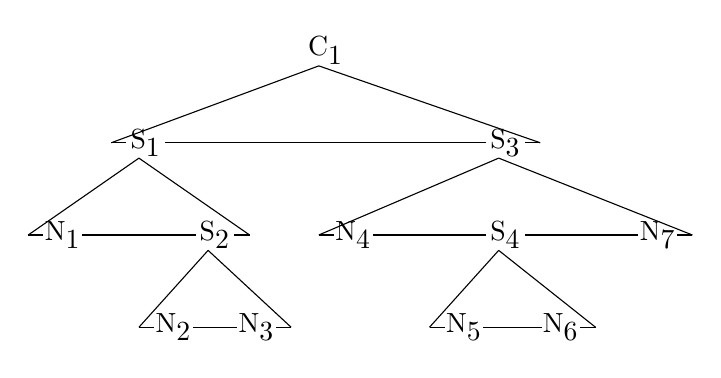
\begin{tikzpicture}
\node at (3.86606,0.) {${\textrm{C}_{\textrm{1}}}$};
\draw (3.778195,-.195255) -- (1.142245,-1.17153);
\draw (1.142245,-1.17153) -- (1.335548,-1.17153);
\draw (1.827592,-1.17153) -- (5.904528,-1.17153);
\draw (6.396572,-1.17153) -- (6.589875,-1.17153);
\draw (6.589875,-1.17153) -- (3.778195,-.195255);
\node at (1.58157,-1.17153) {${\textrm{S}_{\textrm{1}}}$};
\node at (6.15055,-1.17153) {${\textrm{S}_{\textrm{3}}}$};
\draw (1.493705,-1.366785) -- (.087865,-2.34306);
\draw (.087865,-2.34306) -- (.281168,-2.34306);
\draw (.773212,-2.34306) -- (2.214198,-2.34306);
\draw (2.706242,-2.34306) -- (2.899545,-2.34306);
\draw (2.899545,-2.34306) -- (1.493705,-1.366785);
\draw (6.062685,-1.366785) -- (3.778195,-2.34306);
\draw (3.778195,-2.34306) -- (3.971498,-2.34306);
\draw (4.463542,-2.34306) -- (5.904528,-2.34306);
\draw (6.396572,-2.34306) -- (7.837558,-2.34306);
\draw (8.329602,-2.34306) -- (8.522905,-2.34306);
\draw (8.522905,-2.34306) -- (6.062685,-1.366785);
\node at (.52719,-2.34306) {${\textrm{N}_{\textrm{1}}}$};
\node at (2.46022,-2.34306) {${\textrm{S}_{\textrm{2}}}$};
\node at (4.21752,-2.34306) {${\textrm{N}_{\textrm{4}}}$};
\node at (6.15055,-2.34306) {${\textrm{S}_{\textrm{4}}}$};
\node at (8.08358,-2.34306) {${\textrm{N}_{\textrm{7}}}$};
\draw (2.372355,-2.538315) -- (1.493705,-3.51459);
\draw (1.493705,-3.51459) -- (1.687008,-3.51459);
\draw (2.179052,-3.51459) -- (2.741388,-3.51459);
\draw (3.233432,-3.51459) -- (3.426735,-3.51459);
\draw (3.426735,-3.51459) -- (2.372355,-2.538315);
\draw (6.062685,-2.538315) -- (5.184035,-3.51459);
\draw (5.184035,-3.51459) -- (5.377338,-3.51459);
\draw (5.869382,-3.51459) -- (6.607448,-3.51459);
\draw (7.099492,-3.51459) -- (7.292795,-3.51459);
\draw (7.292795,-3.51459) -- (6.062685,-2.538315);
\node at (1.93303,-3.51459) {${\textrm{N}_{\textrm{2}}}$};
\node at (2.98741,-3.51459) {${\textrm{N}_{\textrm{3}}}$};
\node at (5.62336,-3.51459) {${\textrm{N}_{\textrm{5}}}$};
\node at (6.85347,-3.51459) {${\textrm{N}_{\textrm{6}}}$};
\end{tikzpicture}
\bigbreak
\textbf{Figure~3.2. C-S-N Tree}
\end{minipage}
\bigbreak

%%%%%%%%%%%%%%%%%%%%%%%%%%%%%%%%%%%%%%%%%%%%%%%%%%%%%%%%%%%%%%%%

\subsection{Chaining Tables}
\index{chaining!table}

A \textbf{chaining table} contains N-nodes, E-nodes, and one
S-node for keeping track of the chaining table. Link fields
relevant to chaining tables are \texttt{np\symbol{95}link},
\texttt{chain\symbol{95}link}, \texttt{col\symbol{95}link}, \texttt{end\symbol{95}col\symbol{95}link},
\texttt{pred\symbol{95}link}, and \texttt{succ\symbol{95}link}. Chaining tables and
C-S-N trees are connected through their N-nodes. An example of a
chaining table is given in Figure~3.3.

\bigbreak
\begin{minipage}{\textwidth}
\centering
\begin{tikzpicture}
\node at (2.46022,0.) {${\textrm{S}_{\textrm{1}}}$};
\node at (.263595,-1.17153) {${\textrm{N}_{\textrm{1}}}$};
\node at (1.669435,-1.17153) {${\textrm{N}_{\textrm{2}}}$};
\node at (3.075275,-1.17153) {${\textrm{N}_{\textrm{3}}}$};
\node at (4.481115,-1.17153) {${\textrm{N}_{\textrm{4}}}$};
\node at (.263595,-2.34306) {${\textrm{E}_{\textrm{1a}}}$};
\node at (1.669435,-2.34306) {${\textrm{E}_{\textrm{2a}}}$};
\node at (3.075275,-2.34306) {${\textrm{E}_{\textrm{3a}}}$};
\node at (4.481115,-2.34306) {${\textrm{E}_{\textrm{4a}}}$};
\node at (.263595,-3.51459) {${\textrm{E}_{\textrm{1b}}}$};
\node at (1.669435,-3.51459) {${\textrm{E}_{\textrm{2b}}}$};
\node at (.263595,-4.68612) {${\textrm{E}_{\textrm{1c}}}$};
\draw[-Stealth] (2.214198,-.126164769230769) -- (.421752,-1.04536523076923);
\draw[-Stealth] (2.706242,-.149103818181818) -- (4.147228,-1.02242618181818);
\draw[-Stealth] (.421752,-1.17153) -- (1.335548,-1.17153);
\draw[-Stealth] (1.827592,-1.17153) -- (2.741388,-1.17153);
\draw[-Stealth] (3.233432,-1.17153) -- (4.147228,-1.17153);
\draw[-Stealth] (.243093166666667,-1.444887) -- (.243093166666667,-2.069703);
\draw[-Stealth] (.263595,-2.616417) -- (.263595,-3.241233);
\draw[-Stealth] (.263595,-3.787947) -- (.263595,-4.412763);
\draw[-Stealth] (1.64893316666667,-1.444887) -- (1.64893316666667,-2.069703);
\draw[-Stealth] (1.669435,-2.616417) -- (1.669435,-3.241233);
\draw[-Stealth] (3.05477316666667,-1.444887) -- (3.05477316666667,-2.069703);
\draw[-Stealth] (4.46061316666667,-1.444887) -- (4.46061316666667,-2.069703);
\end{tikzpicture}
\bigbreak
\textbf{Figure~3.3. Chaining Table}
\end{minipage}
\bigbreak

%%%%%%%%%%%%%%%%%%%%%%%%%%%%%%%%%%%%%%%%%%%%%%%%%%%%%%%%%%%%%%%%

\subsection{C-Nodes}
\index{node!C-node}

A \textbf{C-node} has the following fields: \texttt{up\symbol{95}link},
\texttt{down\symbol{95}link}, \texttt{left\symbol{95}link}, \texttt{right\symbol{95}link},
\texttt{thread\symbol{95}link}, and \texttt{number}. C-nodes correspond to
conjoined sentences and conjoined subordinate clauses.

%%%%%%%%%%%%%%%%%%%%%%%%%%%%%%%%%%%%%%%%%%%%%%%%%%%%%%%%%%%%%%%%

\subsection{S-Nodes}
\index{node!S-node}

An \textbf{S-node} has exactly the same fields as a C-node and
is only distinguished from a C-node by its
\texttt{NodeId}. S-nodes correspond to sentences and subordinate
clauses.

%%%%%%%%%%%%%%%%%%%%%%%%%%%%%%%%%%%%%%%%%%%%%%%%%%%%%%%%%%%%%%%%

\subsection{N-Nodes}
\index{node!N-node}

An \textbf{N-node} has the following fields: \texttt{lit},
\texttt{ftr}, \texttt{up\symbol{95}link}, \texttt{down\symbol{95}link},
\texttt{thread\symbol{95}link}, \texttt{np\symbol{95}link}, \texttt{chain\symbol{95}link},
\texttt{col\symbol{95}link}, \texttt{end\symbol{95}col\symbol{95}link}, \texttt{pred\symbol{95}link},
\texttt{succ\symbol{95}link}, and \texttt{number}. N-nodes correspond to
noun phrases without attached subordinate clause modifiers.

%%%%%%%%%%%%%%%%%%%%%%%%%%%%%%%%%%%%%%%%%%%%%%%%%%%%%%%%%%%%%%%%

\subsection{E-Nodes}
\index{node!E-node}

An \textbf{E-node} has the following fields: \texttt{sub},
\texttt{ftr}, \texttt{np\symbol{95}link}, \texttt{chain\symbol{95}link}, and
\texttt{col\symbol{95}link}. An E-node may be thought of as a copy of its
\texttt{np\symbol{95}link} with a slightly more defined set of features.

%%%%%%%%%%%%%%%%%%%%%%%%%%%%%%%%%%%%%%%%%%%%%%%%%%%%%%%%%%%%%%%%

\subsection{\textbf{\texttt{lit}} Field}
\index{record field@\texttt{record} field!lit@\texttt{lit}}

The \texttt{lit} field of an N-node is a string pointer to the
string that the N-node represents. The \texttt{lit} field is
actually unnecessary in an N-node, but is convenient for
displaying intermediate results. Function \texttt{view\symbol{95}node\symbol{95}str} of
the Node Processor and some other procedures that display
intermediate results use this field.

%%%%%%%%%%%%%%%%%%%%%%%%%%%%%%%%%%%%%%%%%%%%%%%%%%%%%%%%%%%%%%%%

\subsection{\textbf{\texttt{sub}} Field}
\index{record field@\texttt{record} field!sub@\texttt{sub}}

The \texttt{sub} field of an E-node is a character representing
the subscript of the E-node. The \texttt{sub} field of an
E-node, like the \texttt{lit} field of an N-node, is an
unnecessary field, but is convenient for displaying intermediate
results.

%%%%%%%%%%%%%%%%%%%%%%%%%%%%%%%%%%%%%%%%%%%%%%%%%%%%%%%%%%%%%%%%

\subsection{\textbf{\texttt{ftr}} Field}
\index{record field@\texttt{record} field!ftr@\texttt{ftr}}

The \texttt{ftr} field of an N-node or E-node is an array of
\texttt{Feature}'s representing the feature set of the N-node or
E-node to which it corresponds. A \texttt{Feature} can be a
\texttt{PLUS}, \texttt{MINUS}, or \texttt{QUESTION} as described
in the previous chapter. The offsets \texttt{PNF}, \texttt{FPF},
\texttt{SPF}, \texttt{TPF}, \texttt{PLF}, \texttt{GNF},
\texttt{ANF}, and \texttt{RPF} are used to access elements of
the \texttt{ftr} array. The accessed elements are pronoun
feature, first person feature, second person feature, third
person feature, plural feature, gender feature, animate feature,
and reflexive feature. The number of \texttt{Feature}'s is
\texttt{N\symbol{95}FEATURES}. Figure~3.4 shows some examples of the
settings of \texttt{ftr} for some typical noun phrases.

\bigbreak
\begin{minipage}{\textwidth}
  \centering
  \begin{tabular}{|r|c|c|c|c|c|c|c|c|}
    \hline
    \multicolumn{9}{|c|}{\textbf{Features}} \\
    \hline
    & \textbf{\texttt{PNF}}
    & \textbf{\texttt{FPF}} & \textbf{\texttt{SPF}}
    & \textbf{\texttt{TPF}} & \textbf{\texttt{PLF}}
    & \textbf{\texttt{GNF}} & \textbf{\texttt{ANF}}
    & \textbf{\texttt{RPF}} \\
    \textbf{\texttt{John}} & \texttt{-}
    & \texttt{-} & \texttt{-}
    & \texttt{+} & \texttt{-}
    & \texttt{-} & \texttt{+}
    & \texttt{-} \\
    \textbf{\texttt{flowers}} & \texttt{-}
    & \texttt{-} & \texttt{-}
    & \texttt{+} & \texttt{+}
    & \texttt{?} & \texttt{-}
    & \texttt{-} \\
    \textbf{\texttt{he}} & \texttt{+}
    & \texttt{-} & \texttt{-}
    & \texttt{+} & \texttt{-}
    & \texttt{-} & \texttt{+}
    & \texttt{-} \\
    \textbf{\texttt{them}} & \texttt{+}
    & \texttt{-} & \texttt{-}
    & \texttt{+} & \texttt{+}
    & \texttt{?} & \texttt{?}
    & \texttt{-} \\
    \textbf{\texttt{I}} & \texttt{+}
    & \texttt{+} & \texttt{-}
    & \texttt{-} & \texttt{-}
    & \texttt{?} & \texttt{+}
    & \texttt{-} \\
    \textbf{\texttt{you}} & \texttt{+}
    & \texttt{-} & \texttt{+}
    & \texttt{-} & \texttt{-}
    & \texttt{?} & \texttt{+}
    & \texttt{-} \\
    \textbf{\texttt{her}} & \texttt{+}
    & \texttt{-} & \texttt{-}
    & \texttt{+} & \texttt{-}
    & \texttt{+} & \texttt{+}
    & \texttt{-} \\
    \textbf{\texttt{myself}} & \texttt{+}
    & \texttt{+} & \texttt{-}
    & \texttt{-} & \texttt{-}
    & \texttt{?} & \texttt{+}
    & \texttt{+} \\
    \textbf{\texttt{herself}} & \texttt{+}
    & \texttt{-} & \texttt{-}
    & \texttt{+} & \texttt{-}
    & \texttt{+} & \texttt{+}
    & \texttt{+} \\
    \textbf{\texttt{itself}} & \texttt{+}
    & \texttt{-} & \texttt{-}
    & \texttt{+} & \texttt{-}
    & \texttt{?} & \texttt{-}
    & \texttt{+} \\
    \hline
  \end{tabular}
\end{minipage}
\bigbreak
\textbf{Figure~3.4. \texttt{ftr} Settings for Some Typical Noun Phrases}
\bigbreak

%%%%%%%%%%%%%%%%%%%%%%%%%%%%%%%%%%%%%%%%%%%%%%%%%%%%%%%%%%%%%%%%

\subsection{\textbf{\texttt{up\_link}} Field}
\index{record field@\texttt{record} field!up\symbol{95}link@\texttt{up\symbol{95}link}}

The \texttt{up\symbol{95}link} field of a C-node, S-node, or N-node links
to the parent node of the C-node, S-node, or N-node in the C-S-N
tree in which it occurs. An example of a C-S-N tree with
\texttt{up\symbol{95}link}'s shown is given in Figure~3.5.

\bigbreak
\begin{minipage}{\textwidth}
\centering
\begin{tikzpicture}
\node at (3.69033,0.) {${\textrm{C}_{\textrm{1}}}$};
\node at (1.23011,-1.17153) {${\textrm{S}_{\textrm{1}}}$};
\node at (6.50201,-1.17153) {${\textrm{S}_{\textrm{3}}}$};
\node at (.17573,-2.34306) {${\textrm{N}_{\textrm{1}}}$};
\node at (2.28449,-2.34306) {${\textrm{S}_{\textrm{2}}}$};
\node at (4.39325,-2.34306) {${\textrm{N}_{\textrm{4}}}$};
\node at (6.50201,-2.34306) {${\textrm{S}_{\textrm{4}}}$};
\node at (8.61077,-2.34306) {${\textrm{N}_{\textrm{7}}}$};
\node at (1.58157,-3.51459) {${\textrm{N}_{\textrm{2}}}$};
\node at (2.98741,-3.51459) {${\textrm{N}_{\textrm{3}}}$};
\node at (5.79909,-3.51459) {${\textrm{N}_{\textrm{5}}}$};
\node at (7.20493,-3.51459) {${\textrm{N}_{\textrm{6}}}$};
\draw[-Stealth] (1.476132,-1.054377) -- (3.444308,-.117153);
\draw[-Stealth] (.421752,-2.069703) -- (.984088,-1.444887);
\draw[-Stealth] (2.038468,-2.069703) -- (1.476132,-1.444887);
\draw[-Stealth] (1.74558466666667,-3.241233) -- (2.12047533333333,-2.616417);
\draw[-Stealth] (2.82339533333333,-3.241233) -- (2.44850466666667,-2.616417);
\draw[-Stealth] (6.255988,-1.069021125) -- (3.936352,-.102508875);
\draw[-Stealth] (4.639272,-2.2063815) -- (6.255988,-1.3082085);
\draw[-Stealth] (6.50201,-2.069703) -- (6.50201,-1.444887);
\draw[-Stealth] (5.96310466666667,-3.241233) -- (6.33799533333333,-2.616417);
\draw[-Stealth] (7.04091533333333,-3.241233) -- (6.66602466666667,-2.616417);
\draw[-Stealth] (8.364748,-2.2063815) -- (6.748032,-1.3082085);
\end{tikzpicture}
\bigbreak
\textbf{Figure~3.5. C-S-N Tree with \texttt{up\symbol{95}link}'s Shown}
\end{minipage}
\bigbreak

%%%%%%%%%%%%%%%%%%%%%%%%%%%%%%%%%%%%%%%%%%%%%%%%%%%%%%%%%%%%%%%%

\subsection{\textbf{\texttt{down\_link}} Field}
\index{record field@\texttt{record} field!down\symbol{95}link@\texttt{down\symbol{95}link}}

The \texttt{down\symbol{95}link} field of a C-node, S-node, or N-node links
to the first child node of the C-node, S-node, or N-node in the
C-S-N tree in which it occurs. An example of a C-S-N tree with
\texttt{down\symbol{95}link}'s shown is given in Figure~3.6.

\bigbreak
\begin{minipage}{\textwidth}
\centering
\begin{tikzpicture}
\node at (3.69033,0.) {${\textrm{C}_{\textrm{1}}}$};
\node at (1.23011,-1.17153) {${\textrm{S}_{\textrm{1}}}$};
\node at (6.50201,-1.17153) {${\textrm{S}_{\textrm{3}}}$};
\node at (.17573,-2.34306) {${\textrm{N}_{\textrm{1}}}$};
\node at (2.28449,-2.34306) {${\textrm{S}_{\textrm{2}}}$};
\node at (4.39325,-2.34306) {${\textrm{N}_{\textrm{4}}}$};
\node at (6.50201,-2.34306) {${\textrm{S}_{\textrm{4}}}$};
\node at (8.61077,-2.34306) {${\textrm{N}_{\textrm{7}}}$};
\node at (1.58157,-3.51459) {${\textrm{N}_{\textrm{2}}}$};
\node at (2.98741,-3.51459) {${\textrm{N}_{\textrm{3}}}$};
\node at (5.79909,-3.51459) {${\textrm{N}_{\textrm{5}}}$};
\node at (7.20493,-3.51459) {${\textrm{N}_{\textrm{6}}}$};
\draw[-Stealth] (3.444308,-.117153) -- (1.476132,-1.054377);
\draw[-Stealth] (.984088,-1.444887) -- (.421752,-2.069703);
\draw[-Stealth] (2.12047533333333,-2.616417) -- (1.74558466666667,-3.241233);
\draw[-Stealth] (6.255988,-1.3082085) -- (4.639272,-2.2063815);
\draw[-Stealth] (6.33799533333333,-2.616417) -- (5.96310466666667,-3.241233);
\end{tikzpicture}
\bigbreak
\textbf{Figure~3.6. C-S-N Tree with \texttt{down\symbol{95}link}'s Shown}
\end{minipage}
\bigbreak

%%%%%%%%%%%%%%%%%%%%%%%%%%%%%%%%%%%%%%%%%%%%%%%%%%%%%%%%%%%%%%%%

\subsection{\textbf{\texttt{left\_link}} Field}
\index{record field@\texttt{record} field!left\symbol{95}link@\texttt{left\symbol{95}link}}

The \texttt{left\symbol{95}link} field of a C-node, S-node, or N-node links
to the left brother node of the C-node, S-node, or N-node in the
C-S-N tree in which it occurs. An example of a C-S-N tree with
\texttt{left\symbol{95}link}'s shown is given in Figure~3.7.

\bigbreak
\begin{minipage}{\textwidth}
\centering
\begin{tikzpicture}
\node at (3.69033,0.) {${\textrm{C}_{\textrm{1}}}$};
\node at (1.23011,-1.17153) {${\textrm{S}_{\textrm{1}}}$};
\node at (6.50201,-1.17153) {${\textrm{S}_{\textrm{3}}}$};
\node at (.17573,-2.34306) {${\textrm{N}_{\textrm{1}}}$};
\node at (2.28449,-2.34306) {${\textrm{S}_{\textrm{2}}}$};
\node at (4.39325,-2.34306) {${\textrm{N}_{\textrm{4}}}$};
\node at (6.50201,-2.34306) {${\textrm{S}_{\textrm{4}}}$};
\node at (8.61077,-2.34306) {${\textrm{N}_{\textrm{7}}}$};
\node at (1.58157,-3.51459) {${\textrm{N}_{\textrm{2}}}$};
\node at (2.98741,-3.51459) {${\textrm{N}_{\textrm{3}}}$};
\node at (5.79909,-3.51459) {${\textrm{N}_{\textrm{5}}}$};
\node at (7.20493,-3.51459) {${\textrm{N}_{\textrm{6}}}$};
\draw[-Stealth] (6.255988,-1.17153) -- (1.476132,-1.17153);
\draw[-Stealth] (2.038468,-2.34306) -- (.421752,-2.34306);
\draw[-Stealth] (8.364748,-2.34306) -- (6.748032,-2.34306);
\draw[-Stealth] (6.255988,-2.34306) -- (4.639272,-2.34306);
\draw[-Stealth] (2.741388,-3.51459) -- (1.827592,-3.51459);
\draw[-Stealth] (6.958908,-3.51459) -- (6.045112,-3.51459);
\end{tikzpicture}
\bigbreak
\textbf{Figure~3.7. C-S-N Tree with \texttt{left\symbol{95}link}'s Shown}
\end{minipage}
\bigbreak

%%%%%%%%%%%%%%%%%%%%%%%%%%%%%%%%%%%%%%%%%%%%%%%%%%%%%%%%%%%%%%%%

\subsection{\textbf{\texttt{right\_link}} Field}
\index{record field@\texttt{record} field!right\symbol{95}link@\texttt{right\symbol{95}link}}

The \texttt{right\symbol{95}link} field of a C-node, S-node, or N-node
links to the right brother node of the C-node, S-node, or N-node
in the C-S-N tree in which it occurs. An example of a C-S-N tree
with \texttt{right\symbol{95}link}'s shown is given in Figure~3.8.

\bigbreak
\begin{minipage}{\textwidth}
\centering
\begin{tikzpicture}
\node at (3.69033,0.) {${\textrm{C}_{\textrm{1}}}$};
\node at (1.23011,-1.17153) {${\textrm{S}_{\textrm{1}}}$};
\node at (6.50201,-1.17153) {${\textrm{S}_{\textrm{3}}}$};
\node at (.17573,-2.34306) {${\textrm{N}_{\textrm{1}}}$};
\node at (2.28449,-2.34306) {${\textrm{S}_{\textrm{2}}}$};
\node at (4.39325,-2.34306) {${\textrm{N}_{\textrm{4}}}$};
\node at (6.50201,-2.34306) {${\textrm{S}_{\textrm{4}}}$};
\node at (8.61077,-2.34306) {${\textrm{N}_{\textrm{7}}}$};
\node at (1.58157,-3.51459) {${\textrm{N}_{\textrm{2}}}$};
\node at (2.98741,-3.51459) {${\textrm{N}_{\textrm{3}}}$};
\node at (5.79909,-3.51459) {${\textrm{N}_{\textrm{5}}}$};
\node at (7.20493,-3.51459) {${\textrm{N}_{\textrm{6}}}$};
\draw[-Stealth] (1.476132,-1.17153) -- (6.255988,-1.17153);
\draw[-Stealth] (.421752,-2.34306) -- (2.038468,-2.34306);
\draw[-Stealth] (4.639272,-2.34306) -- (6.255988,-2.34306);
\draw[-Stealth] (6.748032,-2.34306) -- (8.364748,-2.34306);
\draw[-Stealth] (1.827592,-3.51459) -- (2.741388,-3.51459);
\draw[-Stealth] (6.045112,-3.51459) -- (6.958908,-3.51459);
\end{tikzpicture}
\bigbreak
\textbf{Figure~3.8. C-S-N Tree with \texttt{right\symbol{95}link}'s Shown}
\end{minipage}
\bigbreak

%%%%%%%%%%%%%%%%%%%%%%%%%%%%%%%%%%%%%%%%%%%%%%%%%%%%%%%%%%%%%%%%

\subsection{\textbf{\texttt{thread\_link}} Field}
\index{record field@\texttt{record} field!thread\symbol{95}link@\texttt{thread\symbol{95}link}}

The \texttt{thread\symbol{95}link} field of a C-node, S-node, or N-node
links to the first node traversed after the C-node, S-node, or
N-node in a preorder traversal of the C-S-N tree in which it
occurs. An example of a C-S-N tree with \texttt{thread\symbol{95}link}'s
shown is given in Figure~3.9.

\bigbreak
\begin{minipage}{\textwidth}
\centering
\begin{tikzpicture}
\node at (3.69033,0.) {${\textrm{C}_{\textrm{1}}}$};
\node at (1.23011,-1.17153) {${\textrm{S}_{\textrm{1}}}$};
\node (s3) at (6.50201,-1.17153) {${\textrm{S}_{\textrm{3}}}$};
\node at (.17573,-2.34306) {${\textrm{N}_{\textrm{1}}}$};
\node at (2.28449,-2.34306) {${\textrm{S}_{\textrm{2}}}$};
\node at (4.39325,-2.34306) {${\textrm{N}_{\textrm{4}}}$};
\node at (6.50201,-2.34306) {${\textrm{S}_{\textrm{4}}}$};
\node at (8.61077,-2.34306) {${\textrm{N}_{\textrm{7}}}$};
\node at (1.58157,-3.51459) {${\textrm{N}_{\textrm{2}}}$};
\node (n3) at (2.98741,-3.51459) {${\textrm{N}_{\textrm{3}}}$};
\node at (5.79909,-3.51459) {${\textrm{N}_{\textrm{5}}}$};
\node at (7.20493,-3.51459) {${\textrm{N}_{\textrm{6}}}$};
\draw[-Stealth] (3.444308,-.117153) -- (1.476132,-1.054377);
\draw[-Stealth] (.984088,-1.444887) -- (.421752,-2.069703);
\draw[-Stealth] (.421752,-2.34306) -- (2.038468,-2.34306);
\draw[-Stealth] (2.12047533333333,-2.616417) -- (1.74558466666667,-3.241233);
\draw[-Stealth] (1.827592,-3.51459) -- (2.741388,-3.51459);
\draw[-Stealth] (n3.north) to[out=70,in=180] (s3.west);
\draw[-Stealth] (6.255988,-1.3082085) -- (4.639272,-2.2063815);
\draw[-Stealth] (4.639272,-2.34306) -- (6.255988,-2.34306);
\draw[-Stealth] (6.33799533333333,-2.616417) -- (5.96310466666667,-3.241233);
\draw[-Stealth] (6.045112,-3.51459) -- (6.958908,-3.51459);
\draw[-Stealth] (7.450952,-3.30957225) -- (8.364748,-2.54807775);
\end{tikzpicture}
\bigbreak
\textbf{Figure~3.9. C-S-N Tree with \texttt{thread\symbol{95}link}'s Shown}
\end{minipage}
\bigbreak

%%%%%%%%%%%%%%%%%%%%%%%%%%%%%%%%%%%%%%%%%%%%%%%%%%%%%%%%%%%%%%%%

\subsection{\textbf{\texttt{number}} Field}
\index{record field@\texttt{record} field!number@\texttt{number}}

C-node, S-node, or N-node have a \texttt{number} field which is
the number that would be assigned to that node if the nodes of
the C-S-N tree in which it occurs are numbered in a preorder
traversal. An example of a C-S-N tree with \texttt{number}
fields shown is given in Figure~3.10.

\bigbreak
\begin{minipage}{\textwidth}
\centering
\begin{tikzpicture}[
    dotted line/.style={draw, dotted, thick},
    ]
\node at (3.602465,0.) {1};
\node at (1.142245,-1.17153) {2};
\node at (6.414145,-1.17153) {7};
\node at (.087865,-2.34306) {3};
\node at (2.196625,-2.34306) {4};
\node at (4.305385,-2.34306) {8};
\node at (6.414145,-2.34306) {9};
\node at (8.61077,-2.34306) {10};
\node at (1.493705,-3.51459) {5};
\node at (2.899545,-3.51459) {6};
\node at (5.79909,-3.51459) {11};
\node at (7.20493,-3.51459) {12};
\draw[dotted line] (3.479454,-.0585765) -- (1.265256,-1.1129535);
\draw[dotted line] (1.265256,-1.17153) -- (6.291134,-1.17153);
\draw[dotted line] (6.291134,-1.1202755625) -- (3.725476,-.0512544375000001);
\draw[dotted line] (1.019234,-1.3082085) -- (.210876,-2.2063815);
\draw[dotted line] (.210876,-2.34306) -- (2.073614,-2.34306);
\draw[dotted line] (2.073614,-2.2063815) -- (1.265256,-1.3082085);
\draw[dotted line] (2.073614,-2.54807775) -- (1.616716,-3.30957225);
\draw[dotted line] (1.616716,-3.51459) -- (2.776534,-3.51459);
\draw[dotted line] (2.776534,-3.30957225) -- (2.319636,-2.54807775);
\draw[dotted line] (6.291134,-1.23986925) -- (4.428396,-2.27472075);
\draw[dotted line] (4.428396,-2.34306) -- (6.291134,-2.34306);
\draw[dotted line] (6.537156,-2.34306) -- (8.364748,-2.34306);
\draw[dotted line] (8.364748,-2.21184864) -- (6.537156,-1.23713568);
\draw[dotted line] (6.291134,-2.577366) -- (5.94260283333333,-3.241233);
\draw[dotted line] (6.045112,-3.51459) -- (6.958908,-3.51459);
\draw[dotted line] (7.0204135,-3.241233) -- (6.537156,-2.525298);
\end{tikzpicture}
\bigbreak
\textbf{Figure~3.10. C-S-N Tree with \texttt{number} Fields Shown}
\end{minipage}
\bigbreak

%%%%%%%%%%%%%%%%%%%%%%%%%%%%%%%%%%%%%%%%%%%%%%%%%%%%%%%%%%%%%%%%

\subsection{\textbf{\texttt{np\_link}} Field}
\index{record field@\texttt{record} field!np\symbol{95}link@\texttt{np\symbol{95}link}}

For an E-node, the \texttt{np\symbol{95}link} is the N-node to which it is
attached. Conceptually, we think of the E-node as being a copy
of the N-node except for its subscript and different set of
\texttt{Feature}'s, \texttt{chain\symbol{95}link}, and
\texttt{col\symbol{95}link}. The \texttt{np\symbol{95}link} is just a way of avoiding
duplication of information. For an N-node, the \texttt{np\symbol{95}link}
is always itself. An example of a chaining table with
\texttt{np\symbol{95}link}'s shown is given in Figure~3.11.

\bigbreak
\begin{minipage}{\textwidth}
\centering
\begin{tikzpicture}[
    curved arrow/.style={draw, thick, -{Latex[bend]}},
  ]
%nodes
\node (s1) at (2.46022,0.) {${\textrm{S}_{\textrm{1}}}$};
\node (n1) at (.263595,-1.17153) {${\textrm{N}_{\textrm{1}}}$};
\node (n2) at (1.669435,-1.17153) {${\textrm{N}_{\textrm{2}}}$};
\node (n3) at (3.075275,-1.17153) {${\textrm{N}_{\textrm{3}}}$};
\node (n4) at (4.481115,-1.17153) {${\textrm{N}_{\textrm{4}}}$};
\node (e1a) at (.263595,-2.34306) {${\textrm{E}_{\textrm{1a}}}$};
\node (e2a) at (1.669435,-2.34306) {${\textrm{E}_{\textrm{2a}}}$};
\node (e3a) at (3.075275,-2.34306) {${\textrm{E}_{\textrm{3a}}}$};
\node (e4a) at (4.481115,-2.34306) {${\textrm{E}_{\textrm{4a}}}$};
\node (e1b) at (.263595,-3.51459) {${\textrm{E}_{\textrm{1b}}}$};
\node (e2b) at (1.669435,-3.51459) {${\textrm{E}_{\textrm{2b}}}$};
\node (e1c) at (.263595,-4.68612) {${\textrm{E}_{\textrm{1c}}}$};
\draw[-Stealth] (.263595,-2.069703) -- (.263595,-1.444887);
%4 self-loops on n1, n2, n3, n4 .
\draw[curved arrow] (n1) to[out=135, in=45, looseness=4] (n1);
\draw[curved arrow] (n2) to[out=135, in=45, looseness=4] (n2);
\draw[curved arrow] (n3) to[out=135, in=45, looseness=4] (n3);
\draw[curved arrow] (n4) to[out=135, in=45, looseness=4] (n4);
%connections
\draw[-Stealth] (e1b.north west) to[out=135,in=225] (n1.south west);
\draw[-Stealth] (e1c.north west) to[out=135,in=225] (n1.south west);
\draw[-Stealth] (1.669435,-2.069703) -- (1.669435,-1.444887);
\draw[-Stealth] (e2b.north west) to[out=135,in=225] (n2.south west);
\draw[-Stealth] (3.075275,-2.069703) -- (3.075275,-1.444887);
\draw[-Stealth] (4.481115,-2.069703) -- (4.481115,-1.444887);
\end{tikzpicture}
\bigbreak
\textbf{Figure~3.11. Chaining Table with \texttt{up\symbol{95}link}'s Shown}
\end{minipage}
\bigbreak

%%%%%%%%%%%%%%%%%%%%%%%%%%%%%%%%%%%%%%%%%%%%%%%%%%%%%%%%%%%%%%%%

\subsection{\textbf{\texttt{chain\_link}} Field}
\index{record field@\texttt{record} field!chain\symbol{95}link@\texttt{chain\symbol{95}link}}

The \texttt{chain\symbol{95}link} of an E-node is another E-node
representing the substitute to which the first E-node is
attached. When chaining is obligatory, an N-node is chained to
an N-node. An example of a chaining table with
\texttt{chain\symbol{95}link}'s shown is given in Figure~3.12.

\bigbreak
\begin{minipage}{\textwidth}
\centering
\begin{tikzpicture}
%nodes
\node at (2.46022,0.) {${\textrm{S}_{\textrm{1}}}$};
\node at (.263595,-1.17153) {${\textrm{N}_{\textrm{1}}}$};
\node at (1.669435,-1.17153) {${\textrm{N}_{\textrm{2}}}$};
\node at (3.075275,-1.17153) {${\textrm{N}_{\textrm{3}}}$};
\node at (4.481115,-1.17153) {${\textrm{N}_{\textrm{4}}}$};
\node at (.263595,-2.34306) {${\textrm{E}_{\textrm{1a}}}$};
\node at (1.669435,-2.34306) {${\textrm{E}_{\textrm{2a}}}$};
\node at (3.075275,-2.34306) {${\textrm{E}_{\textrm{3a}}}$};
\node (e4a) at (4.481115,-2.34306) {${\textrm{E}_{\textrm{4a}}}$};
\node at (.263595,-3.51459) {${\textrm{E}_{\textrm{1b}}}$};
\node at (1.669435,-3.51459) {${\textrm{E}_{\textrm{2b}}}$};
\node (e1c) at (.263595,-4.68612) {${\textrm{E}_{\textrm{1c}}}$};
%connections
\draw[-Stealth] (.632628,-3.3608266875) -- (2.706242,-2.4968233125);
\draw[-Stealth] (1.99746433333333,-3.241233) -- (2.74724566666667,-2.616417);
\draw[-Stealth] (e1c.east) to[out=20,in=225] (e4a.south west);
\end{tikzpicture}
\bigbreak
\textbf{Figure~3.12. Chaining Table with \texttt{chain\symbol{95}link}'s Shown}
\end{minipage}
\bigbreak

%%%%%%%%%%%%%%%%%%%%%%%%%%%%%%%%%%%%%%%%%%%%%%%%%%%%%%%%%%%%%%%%

\subsection{\textbf{\texttt{col\_link}} Field}
\index{record field@\texttt{record} field!col\symbol{95}link@\texttt{col\symbol{95}link}}

The \texttt{col\symbol{95}link} field of an E-node or N-node links together
the elements of a column in a table. An N-node is always on top
of a column with E-nodes underneath. An example of a chaining
table with \texttt{col\symbol{95}link}'s shown is given in Figure~3.13.

\bigbreak
\begin{minipage}{\textwidth}
\centering
\begin{tikzpicture}
%nodes
\node at (2.46022,0.) {${\textrm{S}_{\textrm{1}}}$};
\node at (.263595,-1.17153) {${\textrm{N}_{\textrm{1}}}$};
\node at (1.669435,-1.17153) {${\textrm{N}_{\textrm{2}}}$};
\node at (3.075275,-1.17153) {${\textrm{N}_{\textrm{3}}}$};
\node at (4.481115,-1.17153) {${\textrm{N}_{\textrm{4}}}$};
\node at (.263595,-2.34306) {${\textrm{E}_{\textrm{1a}}}$};
\node at (1.669435,-2.34306) {${\textrm{E}_{\textrm{2a}}}$};
\node at (3.075275,-2.34306) {${\textrm{E}_{\textrm{3a}}}$};
\node at (4.481115,-2.34306) {${\textrm{E}_{\textrm{4a}}}$};
\node at (.263595,-3.51459) {${\textrm{E}_{\textrm{1b}}}$};
\node at (1.669435,-3.51459) {${\textrm{E}_{\textrm{2b}}}$};
\node at (.263595,-4.68612) {${\textrm{E}_{\textrm{1c}}}$};
%connections
\draw[-Stealth] (.263595,-1.444887) -- (.263595,-2.069703);
\draw[-Stealth] (.263595,-2.616417) -- (.263595,-3.241233);
\draw[-Stealth] (.263595,-3.787947) -- (.263595,-4.412763);
\draw[-Stealth] (1.669435,-1.444887) -- (1.669435,-2.069703);
\draw[-Stealth] (1.669435,-2.616417) -- (1.669435,-3.241233);
\draw[-Stealth] (3.075275,-1.444887) -- (3.075275,-2.069703);
\draw[-Stealth] (4.481115,-1.444887) -- (4.481115,-2.069703);
\end{tikzpicture}
\bigbreak
\textbf{Figure~3.13. Chaining Table with \texttt{col\symbol{95}link}'s Shown}
\end{minipage}
\bigbreak

%%%%%%%%%%%%%%%%%%%%%%%%%%%%%%%%%%%%%%%%%%%%%%%%%%%%%%%%%%%%%%%%

\subsection{\textbf{\texttt{end\_col\_link}} Field}
\index{record field@\texttt{record} field!end\symbol{95}col\symbol{95}link@\texttt{end\symbol{95}col\symbol{95}link}}

The \texttt{end\symbol{95}col\symbol{95}link} field of an N-node
links to the end of the column of E-nodes lying under this
N-node. An example of a chaining table with
\texttt{end\symbol{95}col\symbol{95}link}'s shown is given in
Figure~3.14.

\bigbreak
\begin{minipage}{\textwidth}
\centering
\begin{tikzpicture}
%nodes
\node at (2.46022,0.) {${\textrm{S}_{\textrm{1}}}$};
\node at (.263595,-1.17153) {${\textrm{N}_{\textrm{1}}}$};
\node at (1.669435,-1.17153) {${\textrm{N}_{\textrm{2}}}$};
\node at (3.075275,-1.17153) {${\textrm{N}_{\textrm{3}}}$};
\node at (4.481115,-1.17153) {${\textrm{N}_{\textrm{4}}}$};
\node at (.263595,-2.34306) {${\textrm{E}_{\textrm{1a}}}$};
\node at (1.669435,-2.34306) {${\textrm{E}_{\textrm{2a}}}$};
\node at (3.075275,-2.34306) {${\textrm{E}_{\textrm{3a}}}$};
\node at (4.481115,-2.34306) {${\textrm{E}_{\textrm{4a}}}$};
\node at (.263595,-3.51459) {${\textrm{E}_{\textrm{1b}}}$};
\node at (1.669435,-3.51459) {${\textrm{E}_{\textrm{2b}}}$};
\node at (.263595,-4.68612) {${\textrm{E}_{\textrm{1c}}}$};
%connections
\draw[-Stealth] (n1.south west) to[out=225,in=135] (e1c.north west);
\draw[-Stealth] (n2.south west) to[out=225,in=135] (e2b.north west);
\draw[-Stealth] (3.075275,-1.444887) -- (3.075275,-2.069703);
\draw[-Stealth] (4.481115,-1.444887) -- (4.481115,-2.069703);
\end{tikzpicture}
\bigbreak
\textbf{Figure~3.14. Chaining Table with \texttt{end\symbol{95}col\symbol{95}link}'s Shown}
\end{minipage}
\bigbreak

%%%%%%%%%%%%%%%%%%%%%%%%%%%%%%%%%%%%%%%%%%%%%%%%%%%%%%%%%%%%%%%%

\subsection{\textbf{\texttt{pred\_link}} Field}
\index{record field@\texttt{record} field!pred\symbol{95}link@\texttt{pred\symbol{95}link}}

The \texttt{pred\symbol{95}link} field of an N-node links to the preceding
N-node found in a preorder traversal of the C-S-N tree in which
it occurs. An example of a C-S-N tree with \texttt{pred\symbol{95}link}'s
shown is given in Figure~3.15.

\bigbreak
\begin{minipage}{\textwidth}
\centering
\begin{tikzpicture}
%nodes
\node at (3.69033,0.) {${\textrm{C}_{\textrm{1}}}$};
\node at (1.23011,-1.17153) {${\textrm{S}_{\textrm{1}}}$};
\node at (6.50201,-1.17153) {${\textrm{S}_{\textrm{3}}}$};
\node at (.17573,-2.34306) {${\textrm{N}_{\textrm{1}}}$};
\node at (2.28449,-2.34306) {${\textrm{S}_{\textrm{2}}}$};
\node at (4.39325,-2.34306) {${\textrm{N}_{\textrm{4}}}$};
\node at (6.50201,-2.34306) {${\textrm{S}_{\textrm{4}}}$};
\node at (8.61077,-2.34306) {${\textrm{N}_{\textrm{7}}}$};
\node at (1.58157,-3.51459) {${\textrm{N}_{\textrm{2}}}$};
\node at (2.98741,-3.51459) {${\textrm{N}_{\textrm{3}}}$};
\node at (5.79909,-3.51459) {${\textrm{N}_{\textrm{5}}}$};
\node at (7.20493,-3.51459) {${\textrm{N}_{\textrm{6}}}$};
%connections
\draw[-Stealth] (8.364748,-2.54807775) -- (7.450952,-3.30957225);
\draw[-Stealth] (6.958908,-3.51459) -- (6.045112,-3.51459);
\draw[-Stealth] (5.553068,-3.30957225) -- (4.639272,-2.54807775);
\draw[-Stealth] (4.147228,-2.54807775) -- (3.233432,-3.30957225);
\draw[-Stealth] (2.741388,-3.51459) -- (1.827592,-3.51459);
\draw[-Stealth] (1.335548,-3.30957225) -- (.421752,-2.54807775);
\end{tikzpicture}
\bigbreak
\textbf{Figure~3.15. C-S-N Tree with \texttt{pred\symbol{95}link}'s Shown}
\end{minipage}
\bigbreak

An example of a chaining table with \texttt{pred\symbol{95}link}'s shown is
given in Figure~3.16

\bigbreak
\begin{minipage}{\textwidth}
\centering
\begin{tikzpicture}
%nodes
\node at (2.46022,0.) {${\textrm{S}_{\textrm{1}}}$};
\node at (.263595,-1.17153) {${\textrm{N}_{\textrm{1}}}$};
\node at (1.669435,-1.17153) {${\textrm{N}_{\textrm{2}}}$};
\node at (3.075275,-1.17153) {${\textrm{N}_{\textrm{3}}}$};
\node at (4.481115,-1.17153) {${\textrm{N}_{\textrm{4}}}$};
\node at (.263595,-2.34306) {${\textrm{E}_{\textrm{1a}}}$};
\node at (1.669435,-2.34306) {${\textrm{E}_{\textrm{2a}}}$};
\node at (3.075275,-2.34306) {${\textrm{E}_{\textrm{3a}}}$};
\node at (4.481115,-2.34306) {${\textrm{E}_{\textrm{4a}}}$};
\node at (.263595,-3.51459) {${\textrm{E}_{\textrm{1b}}}$};
\node at (1.669435,-3.51459) {${\textrm{E}_{\textrm{2b}}}$};
\node at (.263595,-4.68612) {${\textrm{E}_{\textrm{1c}}}$};
%connections
\draw[-Stealth] (4.235093,-1.17153) -- (3.321297,-1.17153);
\draw[-Stealth] (2.829253,-1.17153) -- (1.915457,-1.17153);
\draw[-Stealth] (1.423413,-1.17153) -- (.509617,-1.17153);
\end{tikzpicture}
\bigbreak
\textbf{Figure~3.16. Chaining Table with \texttt{pred\symbol{95}link}'s Shown}
\end{minipage}
\bigbreak

%%%%%%%%%%%%%%%%%%%%%%%%%%%%%%%%%%%%%%%%%%%%%%%%%%%%%%%%%%%%%%%%

\subsection{\textbf{\texttt{succ\_link}} Field}
\index{record field@\texttt{record} field!succ\symbol{95}link@\texttt{succ\symbol{95}link}}

The \texttt{succ\symbol{95}link} field of an N-node links to the succeeding
N-node found in a preorder traversal of the C-S-N tree in which
it occurs. An example of a C-S-N tree with \texttt{succ\symbol{95}link}'s
shown is given in Figure~3.17.

\bigbreak
\begin{minipage}{\textwidth}
\centering
\begin{tikzpicture}
%nodes
\node at (3.69033,0.) {${\textrm{C}_{\textrm{1}}}$};
\node at (1.23011,-1.17153) {${\textrm{S}_{\textrm{1}}}$};
\node at (6.50201,-1.17153) {${\textrm{S}_{\textrm{3}}}$};
\node at (.17573,-2.34306) {${\textrm{N}_{\textrm{1}}}$};
\node at (2.28449,-2.34306) {${\textrm{S}_{\textrm{2}}}$};
\node at (4.39325,-2.34306) {${\textrm{N}_{\textrm{4}}}$};
\node at (6.50201,-2.34306) {${\textrm{S}_{\textrm{4}}}$};
\node at (8.61077,-2.34306) {${\textrm{N}_{\textrm{7}}}$};
\node at (1.58157,-3.51459) {${\textrm{N}_{\textrm{2}}}$};
\node at (2.98741,-3.51459) {${\textrm{N}_{\textrm{3}}}$};
\node at (5.79909,-3.51459) {${\textrm{N}_{\textrm{5}}}$};
\node at (7.20493,-3.51459) {${\textrm{N}_{\textrm{6}}}$};
%connections
\draw[-Stealth] (.421752,-2.54807775) -- (1.335548,-3.30957225);
\draw[-Stealth] (1.827592,-3.51459) -- (2.741388,-3.51459);
\draw[-Stealth] (3.233432,-3.30957225) -- (4.147228,-2.54807775);
\draw[-Stealth] (4.639272,-2.54807775) -- (5.553068,-3.30957225);
\draw[-Stealth] (6.045112,-3.51459) -- (6.958908,-3.51459);
\draw[-Stealth] (7.450952,-3.30957225) -- (8.364748,-2.54807775);
\end{tikzpicture}
\bigbreak
\textbf{Figure~3.17. C-S-N Tree with \texttt{succ\symbol{95}link}'s Shown}
\end{minipage}
\bigbreak

An example of a chaining table with \texttt{succ\symbol{95}link}'s shown is
given in Figure~3.18.

\bigbreak
\begin{minipage}{\textwidth}
\centering
\begin{tikzpicture}
%nodes
\node at (2.46022,0.) {${\textrm{S}_{\textrm{1}}}$};
\node at (.263595,-1.17153) {${\textrm{N}_{\textrm{1}}}$};
\node at (1.669435,-1.17153) {${\textrm{N}_{\textrm{2}}}$};
\node at (3.075275,-1.17153) {${\textrm{N}_{\textrm{3}}}$};
\node at (4.481115,-1.17153) {${\textrm{N}_{\textrm{4}}}$};
\node at (.263595,-2.34306) {${\textrm{E}_{\textrm{1a}}}$};
\node at (1.669435,-2.34306) {${\textrm{E}_{\textrm{2a}}}$};
\node at (3.075275,-2.34306) {${\textrm{E}_{\textrm{3a}}}$};
\node at (4.481115,-2.34306) {${\textrm{E}_{\textrm{4a}}}$};
\node at (.263595,-3.51459) {${\textrm{E}_{\textrm{1b}}}$};
\node at (1.669435,-3.51459) {${\textrm{E}_{\textrm{2b}}}$};
\node at (.263595,-4.68612) {${\textrm{E}_{\textrm{1c}}}$};
%connections
\draw[-Stealth] (.509617,-1.17153) -- (1.423413,-1.17153);
\draw[-Stealth] (1.915457,-1.17153) -- (2.829253,-1.17153);
\draw[-Stealth] (3.321297,-1.17153) -- (4.235093,-1.17153);
\end{tikzpicture}
\bigbreak
\textbf{Figure~3.18. Chaining Table with \texttt{succ\symbol{95}link}'s Shown}
\end{minipage}
\bigbreak

%%%%%%%%%%%%%%%%%%%%%%%%%%%%%%%%%%%%%%%%%%%%%%%%%%%%%%%%%%%%%%%%
%
%     Node Processor
%
%%%%%%%%%%%%%%%%%%%%%%%%%%%%%%%%%%%%%%%%%%%%%%%%%%%%%%%%%%%%%%%%

\section{Node Processor}
\index{Node Processor}

The Node Processor module contains functions \texttt{new\symbol{95}c\symbol{95}node},
\texttt{new\symbol{95}s\symbol{95}node}, \texttt{new\symbol{95}n\symbol{95}node}, and \texttt{new\symbol{95}e\symbol{95}node} and
has the skeleton shown below in Figure~4.1.

\bigbreak
\begin{minipage}{\textwidth}
\vbox{\obeylines{\texttt{
\symbol{35}node\symbol{95}proc.py
from~globals~import~*
def~new\symbol{95}c\symbol{95}node()~->~Node:
def~new\symbol{95}s\symbol{95}node()~->~Node:
def~new\symbol{95}n\symbol{95}node()~->~Node:
def~new\symbol{95}e\symbol{95}node()~->~Node:
}}}
\bigbreak
\index{module@\texttt{module}!node\symbol{95}proc@\texttt{node\symbol{95}proc}}
\textbf{Figure~4.1. Skeleton of the Node Processor}
\end{minipage}
\bigbreak

\texttt{new\symbol{95}c\symbol{95}node}, \texttt{new\symbol{95}s\symbol{95}node}, \texttt{new\symbol{95}n\symbol{95}node}, and
\texttt{new\symbol{95}e\symbol{95}node} generate, respectively, a new C-node, S-node,
N-node, or E-node, with their fields initialized and are rather
straightforward functions. These are shown below in
Figures~4.2-4.5.

Function \texttt{new\symbol{95}c\symbol{95}node} returns a new C-node.

\bigbreak
\begin{minipage}{\textwidth}
\vbox{\obeylines{\texttt{
def~new\symbol{95}c\symbol{95}node()~->~Node:
~~~~return~new\symbol{95}node(NodeId.C\symbol{95}NODE)
}}}
\bigbreak
\index{function@\texttt{function}!new\symbol{95}c\symbol{95}node@\texttt{new\symbol{95}c\symbol{95}node}}
\textbf{Figure~4.2. Function \texttt{new\symbol{95}c\symbol{95}node}}
\end{minipage}
\bigbreak

Function \texttt{new\symbol{95}s\symbol{95}node} returns a new S-node.

\bigbreak
\begin{minipage}{\textwidth}
\vbox{\obeylines{\texttt{
def~new\symbol{95}s\symbol{95}node()~->~Node:
~~~~return~new\symbol{95}node(NodeId.S\symbol{95}NODE)
}}}
\bigbreak
\index{function@\texttt{function}!new\symbol{95}s\symbol{95}node@\texttt{new\symbol{95}s\symbol{95}node}}
\textbf{Figure~4.3. Function \texttt{new\symbol{95}s\symbol{95}node}}
\end{minipage}
\bigbreak

Function \texttt{new\symbol{95}n\symbol{95}node} returns a new N-node.

\bigbreak
\begin{minipage}{\textwidth}
\vbox{\obeylines{\texttt{
def~new\symbol{95}n\symbol{95}node()~->~Node:
~~~~answer~=~new\symbol{95}node(NodeId.N\symbol{95}NODE)
~~~~answer.lit~=~""
~~~~answer.ftr~=~[Feature.QUESTION]~*~N\symbol{95}FEATURES
~~~~answer.end\symbol{95}col\symbol{95}link~=~None
~~~~answer.pred\symbol{95}link~=~None
~~~~answer.succ\symbol{95}link~=~None
~~~~answer.np\symbol{95}link~=~answer
~~~~return~answer
}}}
\bigbreak
\index{function@\texttt{function}!new\symbol{95}n\symbol{95}node@\texttt{new\symbol{95}n\symbol{95}node}}
\textbf{Figure~4.4. Function \texttt{new\symbol{95}n\symbol{95}node}}
\end{minipage}
\bigbreak

Function \texttt{new\symbol{95}e\symbol{95}node} returns a new E-node.

\bigbreak
\begin{minipage}{\textwidth}
\vbox{\obeylines{\texttt{
def~new\symbol{95}e\symbol{95}node()~->~Node:
~~~~answer~=~new\symbol{95}node(NodeId.E\symbol{95}NODE)
~~~~answer.sub~=~'~'
~~~~answer.ftr~=~[Feature.QUESTION]~*~N\symbol{95}FEATURES
~~~~return~answer
}}}
\bigbreak
\index{function@\texttt{function}!new\symbol{95}e\symbol{95}node@\texttt{new\symbol{95}e\symbol{95}node}}
\textbf{Figure~4.5. Function \texttt{new\symbol{95}e\symbol{95}node}}
\end{minipage}
\bigbreak

%%%%%%%%%%%%%%%%%%%%%%%%%%%%%%%%%%%%%%%%%%%%%%%%%%%%%%%%%%%%%%%%

\subsection{Function \textbf{\texttt{view\_node\_str}}}

There is one output procedure in the Node Processor that has not
been discussed above that we need to know about, because we will
be looking at some of its output for short while. This is
procedure \texttt{view\symbol{95}node\symbol{95}str} which takes as an argument a
\texttt{NodePointer} and outputs it in readable form.
Otherwise, procedure \texttt{view\symbol{95}node\symbol{95}str} does no processing of its
own, and so we do not need to know the details of its inner
workings. For us it is enough to be able to understand the
output. Function \texttt{view\symbol{95}node\symbol{95}str} has the form indicated in
Figure~4.6.

\bigbreak
\begin{minipage}{\textwidth}
\vbox{\obeylines{\texttt{
def~view\symbol{95}node\symbol{95}str(node:~Node)~->~str:
~~~~"""Formatted~string~representation~of~node."""
~~~~...
}}}
\bigbreak
\index{function@\texttt{function}!view\symbol{95}node\symbol{95}str@\texttt{view\symbol{95}node\symbol{95}str}}
\textbf{Figure~4.6. Skeleton of Function \texttt{view\symbol{95}node\symbol{95}str}}
\end{minipage}
\bigbreak

Some typical output of procedure \texttt{view\symbol{95}node\symbol{95}str} is shown
below in Figure~4.7 where a chaining table is listed.  (Links
from the chaining table to its associated C-S-N tree are also
listed by procedure \texttt{view\symbol{95}node\symbol{95}str}.)

\bigbreak
\begin{minipage}{\textwidth}
  \makebox[\textwidth][c]{
  \begin{tabular}{|r|l|}
    \hline
    \multicolumn{2}{|c|}{\textbf{Nodes}} \\
    \hline
    ${\textbf{\textrm{1}}_{\phantom{z}}}$ & \texttt{\texttt{(C,~up:0,~dn:2,~lt:0,~rt:0,~th:2,~nu:1)}} \\
    ${\textbf{\textrm{2}}_{\phantom{z}}}$ & \texttt{\texttt{(S,~up:1,~dn:3,~lt:0,~rt:5,~th:3,~nu:2)}} \\
    ${\textbf{\textrm{3}}_{\phantom{z}}}$ & \texttt{\texttt{(N,~lit:June,~ftr:[---+-++-],~up:2,~dn:0,}} \\
    & \texttt{\texttt{~lt:0,~rt:4,~th:4,~np:3,~ch:0,~co:${\textrm{3}_{\textrm{a}}}$,~ec:${\textrm{3}_{\textrm{b}}}$,}} \\
    & \texttt{\texttt{~pr:0,~su:4,~nu:3)}} \\
    ${\textbf{\textrm{3}}_{\textbf{\textrm{a}}}}$ & \texttt{\texttt{(E,~sub:A,~ftr:[---+-++-],~np:3,~ch:0,~co:${\textrm{3}_{\textrm{b}}}$)}} \\
    ${\textbf{\textrm{3}}_{\textbf{\textrm{b}}}}$ & \texttt{\texttt{(E,~sub:B,~ftr:[---+-++-],~np:3,~ch:${\textrm{6}_{\textrm{a}}}$,~co:0)}} \\
    ${\textbf{\textrm{4}}_{\phantom{z}}}$ & \texttt{\texttt{(N,~lit:flowers,~ftr:[---++?--],~up:2,~dn:0,}} \\
    & \texttt{\texttt{~lt:3,~rt:0,~th:5,~np:4,~ch:0,~co:${\textrm{4}_{\textrm{a}}}$,~ec:${\textrm{4}_{\textrm{b}}}$,}} \\
    & \texttt{\texttt{~pr:3,~su:6,~nu:4)}} \\
    ${\textbf{\textrm{4}}_{\textbf{\textrm{a}}}}$ & \texttt{\texttt{(E,~sub:A,~ftr:[---++?--],~np:4,~ch:0,~co:${\textrm{4}_{\textrm{b}}}$)}} \\
    ${\textbf{\textrm{4}}_{\textbf{\textrm{b}}}}$ & \texttt{\texttt{(E,~sub:B,~ftr:[---++?--],~np:4,~ch:${\textrm{7}_{\textrm{a}}}$,~co:0)}} \\
    ${\textbf{\textrm{5}}_{\phantom{z}}}$ & \texttt{\texttt{(S,~up:1,~dn:6,~lt:2,~rt:0,~th:6,~nu:5)}} \\
    ${\textbf{\textrm{6}}_{\phantom{z}}}$ & \texttt{\texttt{(N,~lit:she,~ftr:[+--+-++-],~up:5,~dn:0,}} \\
    & \texttt{\texttt{~lt:0,~rt:7,~th:7,~np:6,~ch:0,~co:${\textrm{6}_{\textrm{a}}}$,~ec:${\textrm{6}_{\textrm{a}}}$,}} \\
    & \texttt{\texttt{~pr:4,~su:7,~nu:6)}} \\
    ${\textbf{\textrm{6}}_{\textbf{\textrm{a}}}}$ & \texttt{\texttt{(E,~sub:A,~ftr:[+--+-++-],~np:6,~ch:0,~co:0)}} \\
    ${\textbf{\textrm{7}}_{\phantom{z}}}$ & \texttt{\texttt{(N,~lit:them,~ftr:[+--++??-],~up:5,~dn:0,}} \\
    & \texttt{\texttt{~lt:6,~rt:0,~th:0,~np:7,~ch:0,~co:${\textrm{7}_{\textrm{a}}}$,~ec:${\textrm{7}_{\textrm{a}}}$,}} \\
    & \texttt{\texttt{~pr:6,~su:0,~nu:7)}} \\
    ${\textbf{\textrm{7}}_{\textbf{\textrm{a}}}}$ & \texttt{\texttt{(E,~sub:A,~ftr:[+--++??-],~np:7,~ch:0,~co:0)}} \\
    \hline
  \end{tabular}
  }
\bigbreak
\textbf{Figure~4.7. Typical Output from Function \texttt{view\symbol{95}node\symbol{95}str}}
\end{minipage}
\bigbreak
\noindent(\texttt{C} ${=}$ C-node, \texttt{S} ${=}$ S-node, \texttt{N}
${=}$ N-node, \texttt{E} ${=}$ E-node, \texttt{lit} ${=}$
\texttt{lit} field, \texttt{sub} ${=}$ \texttt{sub} field,
\texttt{ftr} ${=}$ \texttt{ftr} field, \texttt{up} ${=}$
\texttt{up\symbol{95}link}, \texttt{dn} ${=}$ \texttt{down\symbol{95}link},
\texttt{lt} ${=}$ \texttt{left\symbol{95}link}, \texttt{rt} ${=}$
\texttt{right\symbol{95}link}, \texttt{th} ${=}$ \texttt{thread\symbol{95}link},
\texttt{nu} ${=}$ \texttt{number}, \texttt{np} ${=}$
\texttt{np\symbol{95}link}, \texttt{ch} ${=}$ \texttt{chain\symbol{95}link},
\texttt{co} ${=}$ \texttt{col\symbol{95}link}, \texttt{ec} ${=}$
\texttt{end\symbol{95}col\symbol{95}link}, \texttt{pr} ${=}$ \texttt{pred\symbol{95}link}, and
\texttt{su} ${=}$ \texttt{succ\symbol{95}link})

%%%%%%%%%%%%%%%%%%%%%%%%%%%%%%%%%%%%%%%%%%%%%%%%%%%%%%%%%%%%%%%%
%
%     Parser
%
%%%%%%%%%%%%%%%%%%%%%%%%%%%%%%%%%%%%%%%%%%%%%%%%%%%%%%%%%%%%%%%%

\section{Parser}
\index{Parser}

The Parser module defines function \texttt{parse} and has the
form shown below in Figure~5.1.

\bigbreak
\begin{minipage}{\textwidth}
\vbox{\obeylines{\texttt{
\symbol{35}parse\symbol{95}proc.py
from~lexicon~import~*
from~node\symbol{95}proc~import~*
def~parse(obj)~->~Node:
}}}
\bigbreak
\index{module@\texttt{module}!parser@\texttt{parser}}
\textbf{Figure~5.1. Skeleton of the Parser}
\end{minipage}
\bigbreak

\index{system!focus}
\index{system!parse tree}
Function \texttt{parse} accepts as input a \textbf{system focus}
representation and \textbf{system parse tree} that has been
generated by a computer natural language system. The output of
\texttt{parse} is a C-S-N tree incorporating the information
contained in the system parse tree and system focus. The system
focus represents the natural language system's focus of
attention.  This will be gone into in more detail in Chapter~13.

The representation of the system tree inputted to \texttt{parse}
is system dependent, and so the details of \texttt{parse} are
also system dependent. As the internals of \texttt{parse} are
heavily dependent upon and rather involved for any system, we
won't go into the details of \texttt{parse} for any particular
system here.  Hopefully, the reader may glean enough information
from the multitude of examples presented in this thesis to get
an idea of what \texttt{parse} does. In any case, lack of an
actual algorithm for \texttt{parse} isn't so bad since the ideas
presented in this thesis are really still in an early stage and
it is enough to concentrate on them.

Even though the input to the Parser is not well defined, the
output is. The Parser builds from the system parse tree it is
given the corresponding C-S-N tree with all \texttt{up\symbol{95}link}'s,
\texttt{down\symbol{95}link}'s, \texttt{left\symbol{95}link}'s, \texttt{right\symbol{95}link}'s,
\texttt{thread\symbol{95}link}'s, and \texttt{number}'s set to what is
expected. Consider example (5.2) below.

\bigbreak
\begin{minipage}{\textwidth}
\begin{enumerate*}
\item[(5.2)] June hates flowers, but she waters them anyway.
\end{enumerate*}
\bigbreak
\centering
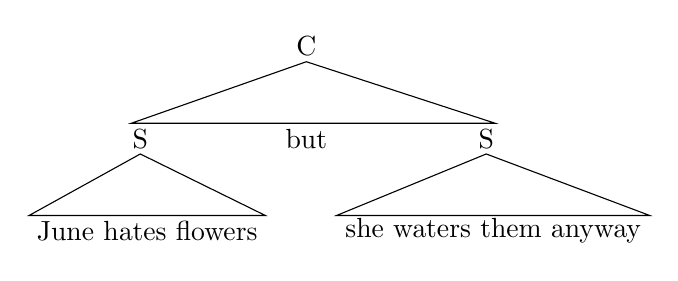
\begin{tikzpicture}
\node at (3.602465,0.) {C};
\draw (3.602465,-.195255) -- (1.38092771748179,-.976275) -- (5.99973228251821,-.976275) -- cycle;
\node at (1.493705,-1.17153) {S};
\node at (3.602465,-1.17153) {but};
\node at (5.886955,-1.17153) {S};
\draw (1.493705,-1.366785) -- (.0816335837976827,-2.147805) -- (3.08150641620232,-2.147805) -- cycle;
\draw (5.886955,-1.366785) -- (3.98712163898279,-2.147805) -- (7.96251836101721,-2.147805) -- cycle;
\node at (1.58157,-2.34306) {June~hates~flowers};
\node at (5.97482,-2.34306) {she~waters~them~anyway};
\end{tikzpicture}
\end{minipage}
\bigbreak

When procedure parse is called on the system parse tree
representing (5.2), we get the following output in Figure~5.3.

\bigbreak
\begin{minipage}{\textwidth}
  \makebox[\textwidth][c]{
  \begin{tabular}{|r|c|c|c|c|c|c|c|c|}
    \hline
    \multicolumn{9}{|c|}{\textbf{Features}} \\
    \hline
    & \textbf{\texttt{PNF}}
    & \textbf{\texttt{FPF}} & \textbf{\texttt{SPF}}
    & \textbf{\texttt{TPF}} & \textbf{\texttt{PLF}}
    & \textbf{\texttt{GNF}} & \textbf{\texttt{ANF}}
    & \textbf{\texttt{RPF}} \\
    \textbf{\texttt{June}} & \texttt{-}
    & \texttt{-} & \texttt{-}
    & \texttt{+} & \texttt{-}
    & \texttt{+} & \texttt{+}
    & \texttt{-} \\
    \textbf{\texttt{flowers}} & \texttt{-}
    & \texttt{-} & \texttt{-}
    & \texttt{+} & \texttt{+}
    & \texttt{?} & \texttt{-}
    & \texttt{-} \\
    \textbf{\texttt{she}} & \texttt{+}
    & \texttt{-} & \texttt{-}
    & \texttt{+} & \texttt{-}
    & \texttt{+} & \texttt{+}
    & \texttt{-} \\
    \textbf{\texttt{them}} & \texttt{+}
    & \texttt{-} & \texttt{-}
    & \texttt{+} & \texttt{+}
    & \texttt{?} & \texttt{?}
    & \texttt{-} \\
    \hline
  \end{tabular}
  }
\end{minipage}
\bigbreak

\bigbreak
\begin{minipage}{\textwidth}
  \makebox[\textwidth][c]{
  \begin{tabular}{|r|l|}
    \hline
    \multicolumn{2}{|c|}{\textbf{Nodes}} \\
    \hline
    ${\textbf{\textrm{1}}_{\phantom{z}}}$ & \texttt{\texttt{(C,~up:0,~dn:2,~lt:0,~rt:0,~th:2,~nu:1)}} \\
    ${\textbf{\textrm{2}}_{\phantom{z}}}$ & \texttt{\texttt{(S,~up:1,~dn:3,~lt:0,~rt:5,~th:3,~nu:2)}} \\
    ${\textbf{\textrm{3}}_{\phantom{z}}}$ & \texttt{\texttt{(N,~lit:June,~ftr:[---+-++-],~up:2,~dn:0,}} \\
    & \texttt{\texttt{~lt:0,~rt:4,~th:4,~np:3,~ch:0,~co:${\textrm{3}_{\textrm{a}}}$,~ec:${\textrm{3}_{\textrm{b}}}$,}} \\
    & \texttt{\texttt{~pr:0,~su:4,~nu:3)}} \\
    ${\textbf{\textrm{4}}_{\phantom{z}}}$ & \texttt{\texttt{(N,~lit:flowers,~ftr:[---++?--],~up:2,~dn:0,}} \\
    & \texttt{\texttt{~lt:3,~rt:0,~th:5,~np:4,~ch:0,~co:${\textrm{4}_{\textrm{a}}}$,~ec:${\textrm{4}_{\textrm{b}}}$,}} \\
    & \texttt{\texttt{~pr:3,~su:6,~nu:4)}} \\
    ${\textbf{\textrm{5}}_{\phantom{z}}}$ & \texttt{\texttt{(S,~up:1,~dn:6,~lt:2,~rt:0,~th:6,~nu:5)}} \\
    ${\textbf{\textrm{6}}_{\phantom{z}}}$ & \texttt{\texttt{(N,~lit:she,~ftr:[+--+-++-],~up:5,~dn:0,}} \\
    & \texttt{\texttt{~lt:0,~rt:7,~th:7,~np:6,~ch:0,~co:${\textrm{6}_{\textrm{a}}}$,~ec:${\textrm{6}_{\textrm{a}}}$,}} \\
    & \texttt{\texttt{~pr:4,~su:7,~nu:6)}} \\
    ${\textbf{\textrm{7}}_{\phantom{z}}}$ & \texttt{\texttt{(N,~lit:them,~ftr:[+--++??-],~up:5,~dn:0,}} \\
    & \texttt{\texttt{~lt:6,~rt:0,~th:0,~np:7,~ch:0,~co:${\textrm{7}_{\textrm{a}}}$,~ec:${\textrm{7}_{\textrm{a}}}$,}} \\
    & \texttt{\texttt{~pr:6,~su:0,~nu:7)}} \\
    \hline
  \end{tabular}
  }
\bigbreak
\textbf{Figure~5.3. Typical Output from \texttt{parse}}
\end{minipage}
\bigbreak

Listing of nodes in Figure~5.3 is done by procedure
\texttt{view\symbol{95}node\symbol{95}str} of the Node Processor described in Chapter~4.
The C-S-N parse tree is slightly more complicated when
focusing is taken into account, but for the time being we will
ignore its effects. We will discuss the effects of focusing on
C-S-N parse trees in Chapter~13.

When Figure~5.3 is drawn as a tree, we get a structure like
Figure~5.4.

\bigbreak
\begin{minipage}{\textwidth}
\centering
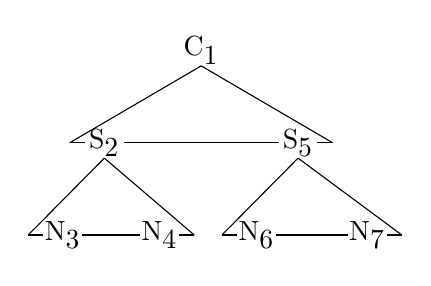
\begin{tikzpicture}
\node at (2.28449,0.) {${\textrm{C}_{\textrm{1}}}$};
\draw (2.28449,-.195255) -- (.615055,-1.17153);
\draw (.615055,-1.17153) -- (.808358,-1.17153);
\draw (1.300402,-1.17153) -- (3.268578,-1.17153);
\draw (3.760622,-1.17153) -- (3.953925,-1.17153);
\draw (3.953925,-1.17153) -- (2.28449,-.195255);
\node at (1.05438,-1.17153) {${\textrm{S}_{\textrm{2}}}$};
\node at (3.5146,-1.17153) {${\textrm{S}_{\textrm{5}}}$};
\draw (1.05438,-1.366785) -- (.087865,-2.34306);
\draw (.087865,-2.34306) -- (.281168,-2.34306);
\draw (.773212,-2.34306) -- (1.511278,-2.34306);
\draw (2.003322,-2.34306) -- (2.196625,-2.34306);
\draw (2.196625,-2.34306) -- (1.05438,-1.366785);
\draw (3.5146,-1.366785) -- (2.548085,-2.34306);
\draw (2.548085,-2.34306) -- (2.741388,-2.34306);
\draw (3.233432,-2.34306) -- (4.147228,-2.34306);
\draw (4.639272,-2.34306) -- (4.832575,-2.34306);
\draw (4.832575,-2.34306) -- (3.5146,-1.366785);
\node at (.52719,-2.34306) {${\textrm{N}_{\textrm{3}}}$};
\node at (1.7573,-2.34306) {${\textrm{N}_{\textrm{4}}}$};
\node at (2.98741,-2.34306) {${\textrm{N}_{\textrm{6}}}$};
\node at (4.39325,-2.34306) {${\textrm{N}_{\textrm{7}}}$};
\end{tikzpicture}
\bigbreak
\textbf{Figure~5.4. Output from \texttt{parse} Drawn as a Tree}
\end{minipage}
\bigbreak

%%%%%%%%%%%%%%%%%%%%%%%%%%%%%%%%%%%%%%%%%%%%%%%%%%%%%%%%%%%%%%%%
%
%     Primary Utilities
%
%%%%%%%%%%%%%%%%%%%%%%%%%%%%%%%%%%%%%%%%%%%%%%%%%%%%%%%%%%%%%%%%

\section{Primary Utilities}
\index{Primary Utilities}

The Primary Utilities module defines the boolean functions
\texttt{precede}, \texttt{command}, and \texttt{separate}
corresponding to the \textit{precedes}, \textit{commands}, and
\textit{is separate from} relations discussed in Chapter~1. The
skeleton of the primary utilitites module is shown below in
Figure~6.1.

\bigbreak
\begin{minipage}{\textwidth}
\vbox{\obeylines{\texttt{
\symbol{35}primary\symbol{95}uty.py
from~globals~import~*
def~precede(n1:~Node,~n2:~Node)~->~bool:
def~command(n1:~Node,~n2:~Node)~->~bool:
def~separate(n1:~Node,~n2:~Node)~->~bool:
}}}
\bigbreak
\index{module@\texttt{module}!primary\symbol{95}uty@\texttt{primary\symbol{95}uty}}
\textbf{Figure~6.1. Skeleton of the Primary Utilities}
\end{minipage}
\bigbreak

The \texttt{precede}, \texttt{command}, and \texttt{separate}
functions do just what is expected. They are \texttt{true} if
and only if the \textit{precedes}, \textit{commands}, and
\textit{is separate from} relations hold between their
arguments. Along with function \texttt{dominate} which is used
by \texttt{separate}, these functions are shown below in Figures
6.2-6.5.

Function \texttt{precede} is \texttt{true} if and only if
\texttt{n1} \textit{precedes} \texttt{n2}.

\bigbreak
\begin{minipage}{\textwidth}
\vbox{\obeylines{\texttt{
def~precede(n1:~Node,~n2:~Node)~->~bool:
~~~~return~n1.number~<~n2.number
}}}
\bigbreak
\index{function@\texttt{function}!precede@\texttt{precede}}
\textbf{Figure~6.2. Function \texttt{precede}}
\end{minipage}
\bigbreak

Function \texttt{dominate} is \texttt{true} if and only if
\texttt{n1} \textit{dominates} \texttt{n2}.

\bigbreak
\begin{minipage}{\textwidth}
\vbox{\obeylines{\texttt{
def~dominate(n1:~Node,~n2:~Node)~->~bool:
~~~~if~n1.number~==~n2.number:
~~~~~~~~return~True
~~~~child~=~n1.down\symbol{95}link
~~~~while~child~is~not~None:
~~~~~~~~if~dominate(child,~n2):
~~~~~~~~~~~~return~True
~~~~~~~~child~=~child.right\symbol{95}link
~~~~return~False
}}}
\bigbreak
\index{function@\texttt{function}!dominate@\texttt{dominate}}
\textbf{Figure~6.3. Function \texttt{dominate}}
\end{minipage}
\bigbreak

Function \texttt{command} is \texttt{true} if and only if
\texttt{n1} \textit{commands} \texttt{n2}.

\bigbreak
\begin{minipage}{\textwidth}
\vbox{\obeylines{\texttt{
def~command(n1:~Node,~n2:~Node)~->~bool:
~~~~return~dominate(n1.up\symbol{95}link,~n2)
}}}
\bigbreak
\index{function@\texttt{function}!command@\texttt{command}}
\textbf{Figure~6.4. Function \texttt{command}}
\end{minipage}
\bigbreak

Function \texttt{separate} is \texttt{true} if and only if
\texttt{n1} \textit{is separate from} \texttt{n2}.

\bigbreak
\begin{minipage}{\textwidth}
\vbox{\obeylines{\texttt{
def~separate(n1:~Node,~n2:~Node)~->~bool:
~~~~parent~=~n1.up\symbol{95}link
~~~~while~not~dominate(parent,~n2):
~~~~~~~~parent~=~parent.up\symbol{95}link
~~~~return~parent.id~==~NodeId.C\symbol{95}NODE
}}}
\bigbreak
\index{function@\texttt{function}!separate@\texttt{separate}}
\textbf{Figure~6.5. Function \texttt{separate}}
\end{minipage}
\bigbreak

%%%%%%%%%%%%%%%%%%%%%%%%%%%%%%%%%%%%%%%%%%%%%%%%%%%%%%%%%%%%%%%%
%
%     Secondary Utilities
%
%%%%%%%%%%%%%%%%%%%%%%%%%%%%%%%%%%%%%%%%%%%%%%%%%%%%%%%%%%%%%%%%

\section{Secondary Utilities}
\index{Secondary Utilities}

The Secondary Utiltities module defines functions \texttt{sc},
\texttt{agr}, and \texttt{rnr}. These stand for Syntactic
Conditions, Agreement, and the Reflexive Nonreflexive Rule. The
skeleton of the Secondary Utilities module is shown below in
Figure~7.1.

\bigbreak
\begin{minipage}{\textwidth}
\vbox{\obeylines{\texttt{
\symbol{35}secondary\symbol{95}uty.py
from~primary\symbol{95}uty~import~*
def~sc(n1:~Node,~n2:~Node)~->~bool:
def~agr(n1:~Node,~n2:~Node)~->~bool:
def~rnr(n1:~Node,~n2:~Node)~->~bool:
}}}
\bigbreak
\index{module@\texttt{module}!secondary\symbol{95}uty@\texttt{secondary\symbol{95}uty}}
\textbf{Figure~7.1. Skeleton of Secondary Utilities}
\end{minipage}
\bigbreak

%%%%%%%%%%%%%%%%%%%%%%%%%%%%%%%%%%%%%%%%%%%%%%%%%%%%%%%%%%%%%%%%

\subsection{Syntactic Conditions}
\index{Syntactic Conditions}

As shown in Chapter~1, certain constraints such as the Precedes
and Commands Rule apply in forward pronominalization.  Function
\texttt{sc} is \texttt{true} whenever these grosser syntactic
constraints are met. In this thesis, we let \texttt{sc} be
\texttt{true} when the Precedes and Commands Rule is satisfied,
function \texttt{sc} is shown below in Figure~7.2.

\bigbreak
\begin{minipage}{\textwidth}
\vbox{\obeylines{\texttt{
def~sc(n1:~Node,~n2:~Node)~->~bool:
~~~~return~not~(precede(n1,~n2)~and~(command(n1,~n2)~or~separate(n1,~n2)))
}}}
\bigbreak
\index{function@\texttt{function}!sc@\texttt{sc}}
\textbf{Figure~7.2. Function \texttt{sc} (Syntactic Conditions)}
\end{minipage}
\bigbreak

%%%%%%%%%%%%%%%%%%%%%%%%%%%%%%%%%%%%%%%%%%%%%%%%%%%%%%%%%%%%%%%%

\subsection{Agreement}
\index{Agreement}

Besides satisfying Syntactic Conditions, there has to be
agreement between a node and its chaining node. First person,
second person, third person, plural, gender, and animate
features have to agree in order for one node to chain to
another. Function \texttt{agr} is shown below in Figure~7.3.

\bigbreak
\begin{minipage}{\textwidth}
\vbox{\obeylines{\texttt{
def~agr(n1:~Node,~n2:~Node)~->~bool:
~~~~ftr1~=~n1.ftr
~~~~ftr2~=~n2.ftr
~~~~return~(eq\symbol{95}feat(ftr1[FeatureIndex.FPF],~ftr2[FeatureIndex.FPF])~and
~~~~~~~~~~~~eq\symbol{95}feat(ftr1[FeatureIndex.SPF],~ftr2[FeatureIndex.SPF])~and
~~~~~~~~~~~~eq\symbol{95}feat(ftr1[FeatureIndex.TPF],~ftr2[FeatureIndex.TPF])~and
~~~~~~~~~~~~eq\symbol{95}feat(ftr1[FeatureIndex.PLF],~ftr2[FeatureIndex.PLF])~and
~~~~~~~~~~~~eq\symbol{95}feat(ftr1[FeatureIndex.GNF],~ftr2[FeatureIndex.GNF])~and
~~~~~~~~~~~~eq\symbol{95}feat(ftr1[FeatureIndex.ANF],~ftr2[FeatureIndex.ANF]))
}}}
\bigbreak
\index{function@\texttt{function}!agr@\texttt{agr}}
\textbf{Figure~7.3. Function \texttt{agr} (Agreement)}
\end{minipage}
\bigbreak

%%%%%%%%%%%%%%%%%%%%%%%%%%%%%%%%%%%%%%%%%%%%%%%%%%%%%%%%%%%%%%%%

\subsection{Equal Features}
\index{Equal Features}

Function \texttt{agr} uses function
\texttt{eq\symbol{95}feat}. \texttt{eq\symbol{95}feat} tests if two \texttt{Feature}'s
are equal. As indicated in Chapter~1, \texttt{Feature}'s are
equal unless a \texttt{PLUS} and \texttt{MINUS} are
compared. Function \texttt{eq\symbol{95}feat} is shown below in Figure~7.4.

\bigbreak
\begin{minipage}{\textwidth}
\vbox{\obeylines{\texttt{
def~eq\symbol{95}feat(f1:~Feature,~f2:~Feature)~->~bool:
~~~~if~f1~==~Feature.PLUS:
~~~~~~~~return~f2~!=~Feature.MINUS
~~~~elif~f1~==~Feature.MINUS:
~~~~~~~~return~f2~!=~Feature.PLUS
~~~~else:~~\symbol{35}~f1~==~Feature.QUESTION
~~~~~~~~return~True
}}}
\bigbreak
\index{function@\texttt{function}!eq\symbol{95}feat@\texttt{eq\symbol{95}feat}}
\textbf{Figure~7.4. Function \texttt{eq\symbol{95}feat} (Equal Features)}
\end{minipage}
\bigbreak

%%%%%%%%%%%%%%%%%%%%%%%%%%%%%%%%%%%%%%%%%%%%%%%%%%%%%%%%%%%%%%%%

\subsection{Reflexive Nonreflexive Rule}
\index{Reflexive Nonreflexive Rule}

The distinction between reflexive pronouns and nonreflexive
pronouns is that reflexive pronouns cannot chain to an N-node
that is outside of the same simplex in which it occurs, while a
nonreflexive pronoun can. This rule will have to be modified
later for genitives, but for now we can suppose that a
nonreflexive pronoun must chain to an N-node outside of the same
simplex in which it is in. Shown in Figure~7.5 is function
\texttt{rnr} which is \texttt{true} when the reflexive
nonreflexive rule is satisfied.

\bigbreak
\begin{minipage}{\textwidth}
\vbox{\obeylines{\texttt{
def~rnr(n1:~Node,~n2:~Node)~->~bool:
~~~~ftr1~=~n1.np\symbol{95}link.ftr
~~~~ftr2~=~n2.np\symbol{95}link.ftr
~~~~if~ftr2[FeatureIndex.GEN]~==~Feature.PLUS:
~~~~~~~~return~False
~~~~elif~ftr1[FeatureIndex.RPF]~==~Feature.PLUS:
~~~~~~~~return~(n1.up\symbol{95}link~==~n2.up\symbol{95}link)
~~~~~~~~~~~~~~~~and~(ftr1[FeatureIndex.GEN]~==~Feature.MINUS)
~~~~elif~ftr1[FeatureIndex.RPF]~==~Feature.MINUS:
~~~~~~~~return~(n1.up\symbol{95}link~!=~n2.up\symbol{95}link)
~~~~~~~~~~~~~~~~or~(ftr1[FeatureIndex.GEN]~!=~Feature.MINUS)
}}}
\bigbreak
\index{function@\texttt{function}!rnr@\texttt{rnr}}
\textbf{Figure~7.5. Function \texttt{rnr} (Reflexive Nonreflexive Rule)}
\end{minipage}
\bigbreak

%%%%%%%%%%%%%%%%%%%%%%%%%%%%%%%%%%%%%%%%%%%%%%%%%%%%%%%%%%%%%%%%
%
%     Table Processor I
%
%%%%%%%%%%%%%%%%%%%%%%%%%%%%%%%%%%%%%%%%%%%%%%%%%%%%%%%%%%%%%%%%

\section{Table Processor I}
\index{Table Processor}

\index{chaining!algorithm|see {function, chaining}}
\index{function@\texttt{function}!chaining@\texttt{chaining}}
The Table Processor module defines function \texttt{chaining}
which takes as input a C-S-N tree and returns its chaining
table. The actions of function \texttt{chaining} in the Table
Processor can only be understood by example, and this is what
this chapter provides. In Chapter~9, we'll look at the actual
algorithms and, in Chapter~10, we'll look at some actual output.

So, let us consider sentence (8.1) below.

\bigbreak
\begin{minipage}{\textwidth}
\begin{enumerate*}
\item[(8.1)] John wants to give June a present, but he isn't
sure she'll like it.
\end{enumerate*}
\bigbreak
\centering
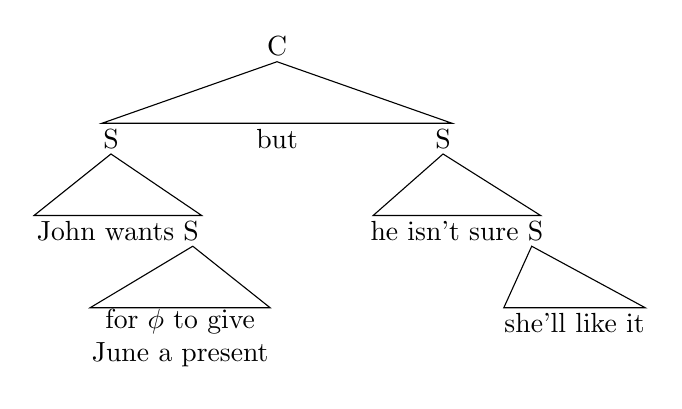
\begin{tikzpicture}
\node at (3.075275,0.) {C};
\draw (3.075275,-.195255) -- (.853737717481786,-.976275) -- (5.29681228251821,-.976275) -- cycle;
\node at (.966515,-1.17153) {S};
\node at (3.075275,-1.17153) {but};
\node at (5.184035,-1.17153) {S};
\draw (.966515,-1.366785) -- (-.00967339767618292,-2.147805) -- (2.11843339767618,-2.147805) -- cycle;
\draw (5.184035,-1.366785) -- (4.29684027443271,-2.147805) -- (6.42268972556729,-2.147805) -- cycle;
\node at (1.05438,-2.34306) {John~wants~S};
\node at (5.359765,-2.34306) {he~isn't~sure~S};
\draw (2.00565611515797,-2.538315) -- (.702731008321334,-3.319335) -- (2.98759899167867,-3.319335) -- cycle;
\draw (6.30991244304908,-2.538315) -- (5.955762977314,-3.319335) -- (7.751177022686,-3.319335) -- cycle;
\node at (1.845165,-3.709845) {\begin{tabular}{cc}
                                 for~${\phi}$~to~give\\
                                 June a present
                               \end{tabular}};
\node at (6.85347,-3.51459) {she'll~like~it};
\end{tikzpicture}
\end{minipage}
\bigbreak

The Parser builds from the system parse tree of (8.1) the
corresponding C-S-N tree with six N-nodes which have the
\texttt{lit} fields and \texttt{ftr}'s indicated below in
Figure~8.2.

\bigbreak
\begin{minipage}{\textwidth}
  \makebox[\textwidth][c]{
  \begin{tabular}{|r|c|c|c|c|c|c|c|c|}
    \hline
    \multicolumn{9}{|c|}{\textbf{Features}} \\
    \hline
    & \textbf{\texttt{PNF}}
    & \textbf{\texttt{FPF}} & \textbf{\texttt{SPF}}
    & \textbf{\texttt{TPF}} & \textbf{\texttt{PLF}}
    & \textbf{\texttt{GNF}} & \textbf{\texttt{ANF}}
    & \textbf{\texttt{RPF}} \\
    \textbf{\texttt{John}} & \texttt{-}
    & \texttt{-} & \texttt{-}
    & \texttt{+} & \texttt{-}
    & \texttt{-} & \texttt{+}
    & \texttt{-} \\
    $\bm{\phi}$ & \texttt{+}
    & \texttt{?} & \texttt{?}
    & \texttt{?} & \texttt{?}
    & \texttt{?} & \texttt{?}
    & \texttt{-} \\
    \textbf{\texttt{June}} & \texttt{-}
    & \texttt{-} & \texttt{-}
    & \texttt{+} & \texttt{-}
    & \texttt{+} & \texttt{+}
    & \texttt{-} \\
    \textbf{\texttt{present}} & \texttt{-}
    & \texttt{-} & \texttt{-}
    & \texttt{+} & \texttt{-}
    & \texttt{?} & \texttt{-}
    & \texttt{-} \\
    \textbf{\texttt{he}} & \texttt{+}
    & \texttt{-} & \texttt{-}
    & \texttt{+} & \texttt{-}
    & \texttt{-} & \texttt{+}
    & \texttt{-} \\
    \textbf{\texttt{she}} & \texttt{+}
    & \texttt{-} & \texttt{-}
    & \texttt{+} & \texttt{-}
    & \texttt{+} & \texttt{+}
    & \texttt{-} \\
    \textbf{\texttt{it}} & \texttt{+}
    & \texttt{-} & \texttt{-}
    & \texttt{+} & \texttt{-}
    & \texttt{?} & \texttt{-}
    & \texttt{-} \\
    \hline
  \end{tabular}
  }
\bigbreak
\textbf{Figure~8.2. \texttt{lit} Fields and \texttt{ftr}'s of the N-Nodes}
\end{minipage}
\bigbreak

The C-S-N tree itself has the form of Figure~8.3 below.

\bigbreak
\begin{minipage}{\textwidth}
\makebox[\textwidth][c]{
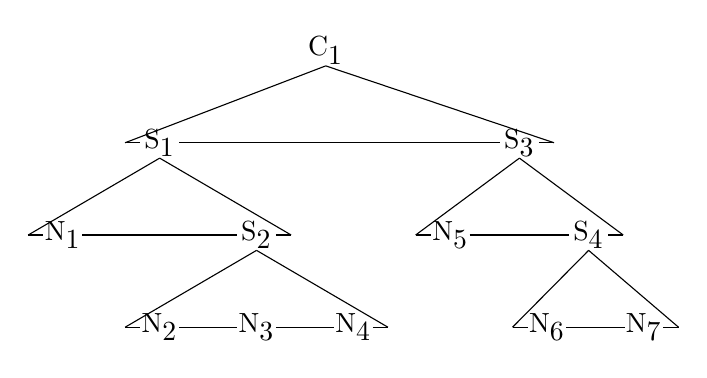
\begin{tikzpicture}
\node at (3.86606,0.) {${\textrm{C}_{\textrm{1}}}$};
\draw (3.86606,-.195255) -- (1.317975,-1.17153);
\draw (1.317975,-1.17153) -- (1.511278,-1.17153);
\draw (2.003322,-1.17153) -- (6.080258,-1.17153);
\draw (6.572302,-1.17153) -- (6.765605,-1.17153);
\draw (6.765605,-1.17153) -- (3.86606,-.195255);
\node at (1.7573,-1.17153) {${\textrm{S}_{\textrm{1}}}$};
\node at (6.32628,-1.17153) {${\textrm{S}_{\textrm{3}}}$};
\draw (1.7573,-1.366785) -- (.087865,-2.34306);
\draw (.087865,-2.34306) -- (.281168,-2.34306);
\draw (.773212,-2.34306) -- (2.741388,-2.34306);
\draw (3.233432,-2.34306) -- (3.426735,-2.34306);
\draw (3.426735,-2.34306) -- (1.7573,-1.366785);
\draw (6.32628,-1.366785) -- (5.008305,-2.34306);
\draw (5.008305,-2.34306) -- (5.201608,-2.34306);
\draw (5.693652,-2.34306) -- (6.958908,-2.34306);
\draw (7.450952,-2.34306) -- (7.644255,-2.34306);
\draw (7.644255,-2.34306) -- (6.32628,-1.366785);
\node at (.52719,-2.34306) {${\textrm{N}_{\textrm{1}}}$};
\node at (2.98741,-2.34306) {${\textrm{S}_{\textrm{2}}}$};
\node at (5.44763,-2.34306) {${\textrm{N}_{\textrm{5}}}$};
\node at (7.20493,-2.34306) {${\textrm{S}_{\textrm{4}}}$};
\draw (2.98741,-2.538315) -- (1.317975,-3.51459);
\draw (1.317975,-3.51459) -- (1.511278,-3.51459);
\draw (2.003322,-3.51459) -- (2.741388,-3.51459);
\draw (3.233432,-3.51459) -- (3.971498,-3.51459);
\draw (4.463542,-3.51459) -- (4.656845,-3.51459);
\draw (4.656845,-3.51459) -- (2.98741,-2.538315);
\draw (7.20493,-2.538315) -- (6.238415,-3.51459);
\draw (6.238415,-3.51459) -- (6.431718,-3.51459);
\draw (6.923762,-3.51459) -- (7.661828,-3.51459);
\draw (8.153872,-3.51459) -- (8.347175,-3.51459);
\draw (8.347175,-3.51459) -- (7.20493,-2.538315);
\node at (1.7573,-3.51459) {${\textrm{N}_{\textrm{2}}}$};
\node at (2.98741,-3.51459) {${\textrm{N}_{\textrm{3}}}$};
\node at (4.21752,-3.51459) {${\textrm{N}_{\textrm{4}}}$};
\node at (6.67774,-3.51459) {${\textrm{N}_{\textrm{6}}}$};
\node at (7.90785,-3.51459) {${\textrm{N}_{\textrm{7}}}$};
\end{tikzpicture}
}
\bigbreak
\textbf{Figure~8.3. C-S-N Parse Tree}
\end{minipage}
\bigbreak

After \texttt{parse} is called, \texttt{chaining} is called. The
first thing to happen is the initialization of the chaining
table for the C-S-N tree. Below each N-node is suspended, by the
\texttt{col\symbol{95}link} of the N-node, a new E-node with subscript
\texttt{A}. Each new E-node has a \texttt{np\symbol{95}link} back to the
N-node it is suspended from. As well, the \texttt{Feature}'s of
each new E-node are copied from the N-node it is suspended
from. Attached to the first and last N-nodes is an S-node to
make it easy to keep track of the first and last N-nodes in the
chaining table. The chaining table, as it looks immediately
after initialization, is shown below in Figure~8.4.

\bigbreak
\begin{minipage}{\textwidth}
\makebox[\textwidth][c]{
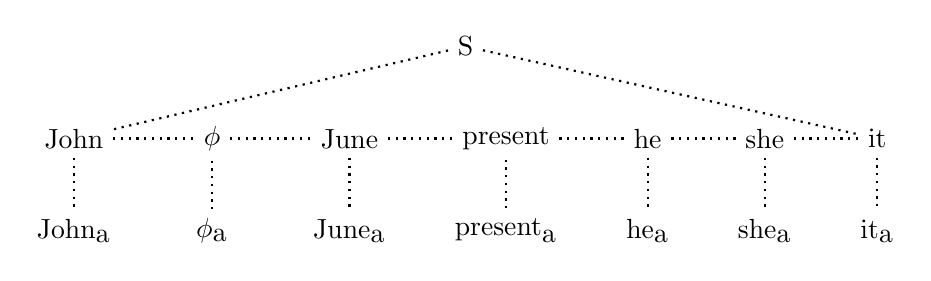
\begin{tikzpicture}[
    every node/.style={align=center},
    dotted line/.style={draw, dotted, thick},
    curved arrow/.style={draw, thick, -{Latex[bend]}},
    ]
\node (S) at (5.478383,0.000000) {S};
\node (John) at (0.505225,-1.171530) {John};
\node (PHI) at (2.259759,-1.171530) {$\phi$};
\node (June) at (4.004530,-1.171530) {June};
\node (present) at (5.992394,-1.171530) {present};
\node (he) at (7.792325,-1.171530) {he};
\node (she) at (9.279357,-1.171530) {she};
\node (it) at (10.707813,-1.171530) {it};
\draw[dotted line] (S) -- (John);
\draw[dotted line] (S) -- (it);
\draw[dotted line] (John) -- (PHI);
\draw[dotted line] (PHI) -- (June);
\draw[dotted line] (June) -- (present);
\draw[dotted line] (present) -- (he);
\draw[dotted line] (he) -- (she);
\draw[dotted line] (she) -- (it);
\node (JohnA) at (0.505225,-2.343060) {${\textrm{John}_{\textrm{a}}}$};
\node (PHIA) at (2.259759,-2.343060) {${\phi_{\textrm{a}}}$};
\node (JuneA) at (4.004530,-2.343060) {${\textrm{June}_{\textrm{a}}}$};
\node (presentA) at (5.992394,-2.343060) {${\textrm{present}_{\textrm{a}}}$};
\node (heA) at (7.792325,-2.343060) {${\textrm{he}_{\textrm{a}}}$};
\node (sheA) at (9.279357,-2.343060) {${\textrm{she}_{\textrm{a}}}$};
\node (itA) at (10.707813,-2.343060) {${\textrm{it}_{\textrm{a}}}$};
\draw[dotted line] (John) -- (JohnA);
\draw[dotted line] (PHI) -- (PHIA);
\draw[dotted line] (June) -- (JuneA);
\draw[dotted line] (present) -- (presentA);
\draw[dotted line] (he) -- (heA);
\draw[dotted line] (she) -- (sheA);
\draw[dotted line] (it) -- (itA);
\end{tikzpicture}
}
\bigbreak
\textbf{Figure~8.4. Chaining Table Immediately after Initialization}
\end{minipage}
\bigbreak

The \texttt{chaining} algorithm works by walking backwards
across N-nodes in the top row and walking down columns of
E-nodes. The \texttt{chaining} algorithm works on two N-nodes at
a time. If the first is compatible with the second under
Syntactic Conditions, Agreement, and the Reflexive Nonreflexive
Rule, then the E-nodes underneath the first N-node that agree
with the second N-node are \texttt{chain\symbol{95}link}'ed to copies of
the second N-node.

The last N-node in the table is \underline{it}, the chaining
table begins with \underline{it}. \underline{it} can't chain to
itself, so the second N-node in the description above becomes
\underline{she} and the \texttt{chaining} algorithm compares
\underline{it} to \underline{she}. Syntactic Conditions are
satisfied, but Agreement isn't.

\bigbreak
\vbox{\obeylines{\texttt{
sc(it,~she)~=~True
agr(it,~she)~=~False
}}}
\bigbreak

The \texttt{chaining} algorithm now moves from \underline{she}
to \underline{he} and compares \underline{it} to
\underline{he}. Again Syntactic Conditions are satisfied, but
Agreement isn't.

\bigbreak
\vbox{\obeylines{\texttt{
sc(it,~he)~=~True
agr(it,~he)~=~False
}}}
\bigbreak

The \texttt{chaining} algorithm moves from \underline{he} to
\underline{present} and compares \underline{it} to
\underline{present}. This time, Syntactic Conditions,
Agreement, and the Reflexive Nonreflexive Rule are satisfied.

\bigbreak
\vbox{\obeylines{\texttt{
sc(it,~present)~=~True
agr(it,~present)~=~True
rnr(it,~present)~=~True
}}}
\bigbreak

\noindent Since all three rules are satisfied, a chain from
\underline{${\textrm{it}_{\textrm{a}}}$} to a copy of \underline{present} may be
created. This happens if \underline{${\textrm{it}_{\textrm{a}}}$} and
\underline{present} agree, and they do.

\bigbreak
\vbox{\obeylines{\texttt{
agr(${\texttt{it}_{\texttt{a}}}$,~present)~=~True
}}}
\bigbreak

The \texttt{chaining} algorithm makes a new E-node copy of
\underline{present}, \underline{${\textrm{present}_{\textrm{b}}}$}, and hangs it
below \underline{present}. The \texttt{chain\symbol{95}link} of
\underline{${\textrm{present}_{\textrm{b}}}$} is set to \underline{${\textrm{it}_{\textrm{a}}}$} and the
semantic features of \underline{${\textrm{it}_{\textrm{a}}}$}, but not the syntactic
features, are copied into the semantic features of
\underline{${\textrm{present}_{\textrm{b}}}$}. After chaining \underline{${\textrm{present}_{\textrm{b}}}$} to
\underline{${\textrm{it}_{\textrm{a}}}$}, the chaining table appears as shown in
Figure~8.5.

\bigbreak
\begin{minipage}{\textwidth}
\makebox[\textwidth][c]{
\begin{tikzpicture}[
    every node/.style={align=center},
    dotted line/.style={draw, dotted, thick},
    curved arrow/.style={draw, thick, -{Latex[bend]}},
    ]
\node (S) at (5.478383,0.000000) {S};
\node (John) at (0.505225,-1.171530) {John};
\node (PHI) at (2.259759,-1.171530) {$\phi$};
\node (June) at (4.004530,-1.171530) {June};
\node (present) at (5.992394,-1.171530) {present};
\node (he) at (7.792325,-1.171530) {he};
\node (she) at (9.279357,-1.171530) {she};
\node (it) at (10.707813,-1.171530) {it};
\draw[dotted line] (S) -- (John);
\draw[dotted line] (S) -- (it);
\draw[dotted line] (John) -- (PHI);
\draw[dotted line] (PHI) -- (June);
\draw[dotted line] (June) -- (present);
\draw[dotted line] (present) -- (he);
\draw[dotted line] (he) -- (she);
\draw[dotted line] (she) -- (it);
\node (JohnA) at (0.505225,-2.343060) {${\textrm{John}_{\textrm{a}}}$};
\node (PHIA) at (2.259759,-2.343060) {${\phi_{\textrm{a}}}$};
\node (JuneA) at (4.004530,-2.343060) {${\textrm{June}_{\textrm{a}}}$};
\node (presentA) at (5.992394,-2.343060) {${\textrm{present}_{\textrm{a}}}$};
\node (heA) at (7.792325,-2.343060) {${\textrm{he}_{\textrm{a}}}$};
\node (sheA) at (9.279357,-2.343060) {${\textrm{she}_{\textrm{a}}}$};
\node (itA) at (10.707813,-2.343060) {${\textrm{it}_{\textrm{a}}}$};
\draw[dotted line] (John) -- (JohnA);
\draw[dotted line] (PHI) -- (PHIA);
\draw[dotted line] (June) -- (JuneA);
\draw[dotted line] (present) -- (presentA);
\draw[dotted line] (he) -- (heA);
\draw[dotted line] (she) -- (sheA);
\draw[dotted line] (it) -- (itA);
\node (presentB) at (5.992394,-3.514590) {${\textrm{present}_{\textrm{b}}}$};
\draw[dotted line] (presentA) -- (presentB);
\draw[curved arrow] (presentB.north east) to [out=28.62,in=-151.38] (itA.south west);
\end{tikzpicture}
}
\bigbreak
\textbf{Figure~8.5. Chaining Table after Chaining \underline{${\textrm{present}_{\textrm{b}}}$} to \underline{${\textrm{it}_{\textrm{a}}}$}}
\end{minipage}
\bigbreak

The \texttt{chaining} algorithm now moves from \underline{present} to
\underline{June}. Syntactic Conditions are satisfied, but Agreement
isn't.

\bigbreak
\vbox{\obeylines{\texttt{
sc(it,~June)~=~True
agr(it,~June)~=~False
}}}
\bigbreak

The \texttt{chaining} algorithm now moves from \underline{June}
to \underline{${\phi}$}.  This time, all three rules, Syntactic
Conditions, Agreement, and the Reflexive Nonreflexive Rule are
satisfied.

\bigbreak
\vbox{\obeylines{\texttt{
sc(it,~${\phi}$)~=~True
agr(it,~${\phi}$)~=~True
rnr(it,~${\phi}$)~=~True
}}}
\bigbreak

\noindent Since all three rules are satisfied, E-nodes under
\underline{it} that agree with \underline{${\phi}$} chain to copies
of \underline{${\phi}$}. \underline{${\textrm{it}_{\textrm{a}}}$} is compared to
\underline{${\phi}$}, and it is seen that they agree.

\bigbreak
\vbox{\obeylines{\texttt{
agr(${\texttt{it}_{\texttt{a}}}$,~${\phi}$)~=~True
}}}
\bigbreak

\noindent The \texttt{chaining} algorithm makes a new E-node
copy of \underline{${\phi}$}, \underline{${\phi_{\textrm{b}}}$}, and hangs it below
\underline{${\phi}$}. The \texttt{chain\symbol{95}link} of \underline{${\phi_{\textrm{b}}}$} is
set to \underline{${\textrm{it}_{\textrm{a}}}$} and the semantic features of
\underline{${\textrm{it}_{\textrm{a}}}$} are copied into the semantic features of
\underline{${\phi_{\textrm{b}}}$}. After chaining \underline{${\phi_{\textrm{b}}}$} to
\underline{${\textrm{it}_{\textrm{a}}}$}, the chaining table appears as shown in
Figure~8.6.

\bigbreak
\begin{minipage}{\textwidth}
\makebox[\textwidth][c]{
\begin{tikzpicture}[
    every node/.style={align=center},
    dotted line/.style={draw, dotted, thick},
    curved arrow/.style={draw, thick, -{Latex[bend]}},
    ]
\node (S) at (5.478383,0.000000) {S};
\node (John) at (0.505225,-1.171530) {John};
\node (PHI) at (2.259759,-1.171530) {$\phi$};
\node (June) at (4.004530,-1.171530) {June};
\node (present) at (5.992394,-1.171530) {present};
\node (he) at (7.792325,-1.171530) {he};
\node (she) at (9.279357,-1.171530) {she};
\node (it) at (10.707813,-1.171530) {it};
\draw[dotted line] (S) -- (John);
\draw[dotted line] (S) -- (it);
\draw[dotted line] (John) -- (PHI);
\draw[dotted line] (PHI) -- (June);
\draw[dotted line] (June) -- (present);
\draw[dotted line] (present) -- (he);
\draw[dotted line] (he) -- (she);
\draw[dotted line] (she) -- (it);
\node (JohnA) at (0.505225,-2.343060) {${\textrm{John}_{\textrm{a}}}$};
\node (PHIA) at (2.259759,-2.343060) {${\phi_{\textrm{a}}}$};
\node (JuneA) at (4.004530,-2.343060) {${\textrm{June}_{\textrm{a}}}$};
\node (presentA) at (5.992394,-2.343060) {${\textrm{present}_{\textrm{a}}}$};
\node (heA) at (7.792325,-2.343060) {${\textrm{he}_{\textrm{a}}}$};
\node (sheA) at (9.279357,-2.343060) {${\textrm{she}_{\textrm{a}}}$};
\node (itA) at (10.707813,-2.343060) {${\textrm{it}_{\textrm{a}}}$};
\draw[dotted line] (John) -- (JohnA);
\draw[dotted line] (PHI) -- (PHIA);
\draw[dotted line] (June) -- (JuneA);
\draw[dotted line] (present) -- (presentA);
\draw[dotted line] (he) -- (heA);
\draw[dotted line] (she) -- (sheA);
\draw[dotted line] (it) -- (itA);
\node (PHIB) at (2.259759,-3.514590) {${\phi_{\textrm{b}}}$};
\node (presentB) at (5.992394,-3.514590) {${\textrm{present}_{\textrm{b}}}$};
\draw[dotted line] (PHIA) -- (PHIB);
\draw[dotted line] (presentA) -- (presentB);
\draw[curved arrow] (presentB.north east) to [out=28.62,in=-109.00] (itA.south);
\draw[curved arrow] (PHIB.east) to [out=18.13,in=155.75] (itA.north west);
\end{tikzpicture}
}
\bigbreak
\textbf{Figure~8.6. Chaining Table After Chaining \underline{${\phi_{\textrm{b}}}$} to \underline{${\textrm{it}_{\textrm{a}}}$}}
\end{minipage}
\bigbreak

The \texttt{chaining} algorithm now moves to \underline{John}
and compares \underline{John} to \underline{it}. Syntactic
Conditions hold, but Agreement does not.

\bigbreak
\vbox{\obeylines{\texttt{
sc(it,~John)~=~True
agr(it,~John)~=~False
}}}
\bigbreak

\noindent Having exhausted all possible combinations with
\underline{it}, the \texttt{chaining} algorithm considers
\underline{she}.

The \texttt{chaining} algorithm tries comparing \underline{she}
to \underline{it}, but Syntactic Conditions are not satisfied.

\bigbreak
\vbox{\obeylines{\texttt{
sc(she,~it)~=~False
}}}
\bigbreak

The \texttt{chaining} algorithm moves from \underline{it} to
\underline{she}, but \underline{she} can't chain to
\underline{she}, so the \texttt{chaining} algorithm moves to
\underline{he}.  This time Syntactic Conditions are satisfied,
but Agreement isn't.

\bigbreak
\vbox{\obeylines{\texttt{
sc(she,~he)~=~True
agr(she,~he)~=~False
}}}
\bigbreak

The \texttt{chaining} algorithm now moves from \underline{he} to
\underline{present} where again Syntactic Conditions are
satisfied, but Agreement isn't.

\bigbreak
\vbox{\obeylines{\texttt{
sc(she,~present)~=~True
agr(she,~present)~=~False
}}}
\bigbreak

The \texttt{chaining} algorithm moves from \underline{present}
to \underline{June}.  This time all three rules are satisfied.

\bigbreak
\vbox{\obeylines{\texttt{
sc(she,~June)~=~True
agr(she,~June)~=~True
rnr(she,~June)~=~True
}}}
\bigbreak

\noindent As all three rules are satisfied, E-nodes under
\underline{she} that agree with \underline{June} chain to copies
of \underline{June}. \underline{${\textrm{she}_{\textrm{a}}}$} is compared to
\underline{June}, and it is seen that they agree.

\bigbreak
\vbox{\obeylines{\texttt{
agr(${\texttt{she}_{\texttt{a}}}$,~June)~=~True
}}}
\bigbreak

\noindent The \texttt{chaining} algorithm makes a new E-node
copy of \underline{June}, \underline{${\textrm{June}_{\textrm{b}}}$}, and hangs it below
\underline{June}. The \texttt{chain\symbol{95}link} of \underline{${\textrm{June}_{\textrm{b}}}$} is
set to \underline{${\textrm{she}_{\textrm{a}}}$} and the semantic features of
\underline{${\textrm{she}_{\textrm{a}}}$} are copied into the semantic features of
\underline{${\textrm{June}_{\textrm{b}}}$}. After chaining \underline{${\textrm{June}_{\textrm{b}}}$} to
\underline{${\textrm{she}_{\textrm{a}}}$}, the chaining table appears as shown in
Figure~8.7.

\bigbreak
\begin{minipage}{\textwidth}
\makebox[\textwidth][c]{
\begin{tikzpicture}[
    every node/.style={align=center},
    dotted line/.style={draw, dotted, thick},
    curved arrow/.style={draw, thick, -{Latex[bend]}},
    ]
\node (S) at (5.478383,0.000000) {S};
\node (John) at (0.505225,-1.171530) {John};
\node (PHI) at (2.259759,-1.171530) {$\phi$};
\node (June) at (4.004530,-1.171530) {June};
\node (present) at (5.992394,-1.171530) {present};
\node (he) at (7.792325,-1.171530) {he};
\node (she) at (9.279357,-1.171530) {she};
\node (it) at (10.707813,-1.171530) {it};
\draw[dotted line] (S) -- (John);
\draw[dotted line] (S) -- (it);
\draw[dotted line] (John) -- (PHI);
\draw[dotted line] (PHI) -- (June);
\draw[dotted line] (June) -- (present);
\draw[dotted line] (present) -- (he);
\draw[dotted line] (he) -- (she);
\draw[dotted line] (she) -- (it);
\node (JohnA) at (0.505225,-2.343060) {${\textrm{John}_{\textrm{a}}}$};
\node (PHIA) at (2.259759,-2.343060) {${\phi_{\textrm{a}}}$};
\node (JuneA) at (4.004530,-2.343060) {${\textrm{June}_{\textrm{a}}}$};
\node (presentA) at (5.992394,-2.343060) {${\textrm{present}_{\textrm{a}}}$};
\node (heA) at (7.792325,-2.343060) {${\textrm{he}_{\textrm{a}}}$};
\node (sheA) at (9.279357,-2.343060) {${\textrm{she}_{\textrm{a}}}$};
\node (itA) at (10.707813,-2.343060) {${\textrm{it}_{\textrm{a}}}$};
\draw[dotted line] (John) -- (JohnA);
\draw[dotted line] (PHI) -- (PHIA);
\draw[dotted line] (June) -- (JuneA);
\draw[dotted line] (present) -- (presentA);
\draw[dotted line] (he) -- (heA);
\draw[dotted line] (she) -- (sheA);
\draw[dotted line] (it) -- (itA);
\node (PHIB) at (2.259759,-3.514590) {${\phi_{\textrm{b}}}$};
\node (JuneB) at (4.004530,-3.514590) {${\textrm{June}_{\textrm{b}}}$};
\node (presentB) at (5.992394,-3.514590) {${\textrm{present}_{\textrm{b}}}$};
\draw[dotted line] (PHIA) -- (PHIB);
\draw[dotted line] (JuneA) -- (JuneB);
\draw[dotted line] (presentA) -- (presentB);
\draw[curved arrow] (presentB.north east) to [out=28.62,in=-109.00] (itA.south);
\draw[curved arrow] (PHIB.east) to [out=18.13,in=155.75] (itA.north west);
\draw[curved arrow] (JuneB.north east) to [out=28.62,in=-151.38] (sheA.south west);
\end{tikzpicture}
}
\bigbreak
\textbf{Figure~8.7. Chaining Table after Chaining \underline{${\textrm{June}_{\textrm{b}}}$} to \underline{${\textrm{she}_{\textrm{a}}}$}}
\end{minipage}
\bigbreak

The \texttt{chaining} algorithm now moves from \underline{June}
to \underline{${\phi}$} and compares \underline{she} to
\underline{${\phi}$}. All three rules are satisfied.

\bigbreak
\vbox{\obeylines{\texttt{
sc(she,~$\phi$)~=~True
agr(she,~$\phi$)~=~True
rnr(she,~$\phi$)~=~True
}}}
\bigbreak

Copies of \underline{${\phi}$} are \texttt{chain\symbol{95}link}'ed to E-nodes
under \underline{she} that agree with
\underline{${\phi}$}. \underline{${\textrm{she}_{\textrm{a}}}$} is compared to
\underline{${\phi}$}, and it is seen that they agree.

\bigbreak
\vbox{\obeylines{\texttt{
agr(${\texttt{she}_{\texttt{a}}}$,~$\phi$)~=~True
}}}
\bigbreak

\noindent A new E-node copy of \underline{${\phi}$},
\underline{${\phi_{\textrm{c}}}$}, is made and hung below \underline{${\phi}$}.  The
\texttt{chain\symbol{95}link} of \underline{${\phi_{\textrm{c}}}$} is set to
\underline{${\textrm{she}_{\textrm{a}}}$} and the semantic features of \underline{${\textrm{she}_{\textrm{a}}}$}
are copied into the semantic features of \underline{${\phi_{\textrm{c}}}$}. After
chaining \underline{${\phi_{\textrm{c}}}$} to \underline{${\textrm{she}_{\textrm{a}}}$}, the chaining
table appears as shown in Figure~8.8.

\bigbreak
\begin{minipage}{\textwidth}
\makebox[\textwidth][c]{
\begin{tikzpicture}[
    every node/.style={align=center},
    dotted line/.style={draw, dotted, thick},
    curved arrow/.style={draw, thick, -{Latex[bend]}},
    ]
\node (S) at (5.478383,0.000000) {S};
\node (John) at (0.505225,-1.171530) {John};
\node (PHI) at (2.259759,-1.171530) {$\phi$};
\node (June) at (4.004530,-1.171530) {June};
\node (present) at (5.992394,-1.171530) {present};
\node (he) at (7.792325,-1.171530) {he};
\node (she) at (9.279357,-1.171530) {she};
\node (it) at (10.707813,-1.171530) {it};
\draw[dotted line] (S) -- (John);
\draw[dotted line] (S) -- (it);
\draw[dotted line] (John) -- (PHI);
\draw[dotted line] (PHI) -- (June);
\draw[dotted line] (June) -- (present);
\draw[dotted line] (present) -- (he);
\draw[dotted line] (he) -- (she);
\draw[dotted line] (she) -- (it);
\node (JohnA) at (0.505225,-2.343060) {${\textrm{John}_{\textrm{a}}}$};
\node (PHIA) at (2.259759,-2.343060) {${\phi_{\textrm{a}}}$};
\node (JuneA) at (4.004530,-2.343060) {${\textrm{June}_{\textrm{a}}}$};
\node (presentA) at (5.992394,-2.343060) {${\textrm{present}_{\textrm{a}}}$};
\node (heA) at (7.792325,-2.343060) {${\textrm{he}_{\textrm{a}}}$};
\node (sheA) at (9.279357,-2.343060) {${\textrm{she}_{\textrm{a}}}$};
\node (itA) at (10.707813,-2.343060) {${\textrm{it}_{\textrm{a}}}$};
\draw[dotted line] (John) -- (JohnA);
\draw[dotted line] (PHI) -- (PHIA);
\draw[dotted line] (June) -- (JuneA);
\draw[dotted line] (present) -- (presentA);
\draw[dotted line] (he) -- (heA);
\draw[dotted line] (she) -- (sheA);
\draw[dotted line] (it) -- (itA);
\node (PHIB) at (2.259759,-3.514590) {${\phi_{\textrm{b}}}$};
\node (JuneB) at (4.004530,-3.514590) {${\textrm{June}_{\textrm{b}}}$};
\node (presentB) at (5.992394,-3.514590) {${\textrm{present}_{\textrm{b}}}$};
\draw[dotted line] (PHIA) -- (PHIB);
\draw[dotted line] (JuneA) -- (JuneB);
\draw[dotted line] (presentA) -- (presentB);
\node (PHIC) at (2.259759,-4.686120) {${\phi_{\textrm{c}}}$};
\draw[dotted line] (PHIB) -- (PHIC);
\draw[curved arrow] (presentB.north east) to [out=28.62,in=-109.00] (itA.south);
\draw[curved arrow] (PHIB.east) to [out=18.13,in=155.75] (itA.north west);
\draw[curved arrow] (PHIC.north east) to [out=39.31,in=-98.36] (sheA.south);
\draw[curved arrow] (JuneB.north east) to [out=28.62,in=166.29] (sheA.west);
\end{tikzpicture}
}
\bigbreak
\textbf{Figure~8.8. Chaining Table after Chaining \underline{${\phi_{\textrm{c}}}$} to \underline{${\textrm{she}_{\textrm{a}}}$}}
\end{minipage}
\bigbreak

The \texttt{chaining} algorithm now moves from \underline{${\phi}$}
to \underline{John} and compares \underline{she} to
\underline{John}. It is seen that Syntactic Conditions are
satisfied, but Agreement isn't.

\bigbreak
\vbox{\obeylines{\texttt{
sc(she,~John)~=~True
agr(she,~John)~=~False
}}}
\bigbreak

\noindent This completes the creation of \texttt{chain\symbol{95}link}'s to
E-nodes under \underline{she}. The \texttt{chaining} algorithm
now considers \underline{he}.

\underline{he} is compared to \underline{it}, but it is seen
that Syntactic Conditions aren't satisfied.

\bigbreak
\vbox{\obeylines{\texttt{
sc(he,~it)~=~False
}}}
\bigbreak

The \texttt{chaining} algorithm moves from \underline{it} to
\underline{she}, but again, Syntactic Conditions aren't
satisfied.

\bigbreak
\vbox{\obeylines{\texttt{
sc(he,~she)~=~False
}}}
\bigbreak

The \texttt{chaining} algorithm moves from \underline{she} to
\underline{he}, but \underline{he} can't chain to
\underline{he}, so the \texttt{chaining} algorithm moves from
\underline{he} to \underline{present}. This time Syntactic
Conditions are satisfied, but Agreement isn't.

\bigbreak
\vbox{\obeylines{\texttt{
sc(he,~present)~=~True
agr(he,~present)~=~False
}}}
\bigbreak

The \texttt{chaining} algorithm moves from \underline{present}
to \underline{June}, and similar results happen.

\bigbreak
\vbox{\obeylines{\texttt{
sc(he,~June)~=~True
agr(he,~June)~=~False
}}}
\bigbreak

Next, the \texttt{chaining} algorithm moves from
\underline{June} to \underline{${\phi}$}, and, this time, all three
rules, Syntactic Conditions, Agreement, and the Reflexive
Nonreflexive Rule, are satisfied.

\bigbreak
\vbox{\obeylines{\texttt{
sc(he,~$\phi$)~=~True
agr(he,~$\phi$)~=~True
rnr(he,~$\phi$)~=~True
}}}
\bigbreak

\noindent Copies of \underline{he} are \texttt{chain\symbol{95}link}'ed to
E-nodes under \underline{${\phi}$} that agree with
\underline{he}. \underline{${\textrm{he}_{\textrm{a}}}$} is compared to \underline{${\phi}$},
and it is seen that they agree.

\bigbreak
\vbox{\obeylines{\texttt{
agr(${\texttt{he}_{\texttt{a}}}$,~$\phi$)~=~True
}}}
\bigbreak

\noindent A new E-node copy of \underline{${\phi}$},
\underline{${\phi_{\textrm{d}}}$}, is made and hung below \underline{${\phi}$}.  The
\texttt{chain\symbol{95}link} of \underline{${\phi_{\textrm{d}}}$} is set to \underline{${\textrm{he}_{\textrm{a}}}$}
and the semantic features of \underline{${\textrm{he}_{\textrm{a}}}$} are copied into the
semantic features of \underline{${\phi_{\textrm{d}}}$}. After chaining
\underline{${\phi_{\textrm{d}}}$} to \underline{${\textrm{he}_{\textrm{a}}}$}, the chaining table appears
as shown in Figure~8.9.

\bigbreak
\begin{minipage}{\textwidth}
\makebox[\textwidth][c]{
\begin{tikzpicture}[
    every node/.style={align=center},
    dotted line/.style={draw, dotted, thick},
    curved arrow/.style={draw, thick, -{Latex[bend]}},
    ]
\node (S) at (5.478383,0.000000) {S};
\node (John) at (0.505225,-1.171530) {John};
\node (PHI) at (2.259759,-1.171530) {$\phi$};
\node (June) at (4.004530,-1.171530) {June};
\node (present) at (5.992394,-1.171530) {present};
\node (he) at (7.792325,-1.171530) {he};
\node (she) at (9.279357,-1.171530) {she};
\node (it) at (10.707813,-1.171530) {it};
\draw[dotted line] (S) -- (John);
\draw[dotted line] (S) -- (it);
\draw[dotted line] (John) -- (PHI);
\draw[dotted line] (PHI) -- (June);
\draw[dotted line] (June) -- (present);
\draw[dotted line] (present) -- (he);
\draw[dotted line] (he) -- (she);
\draw[dotted line] (she) -- (it);
\node (JohnA) at (0.505225,-2.343060) {${\textrm{John}_{\textrm{a}}}$};
\node (PHIA) at (2.259759,-2.343060) {${\phi_{\textrm{a}}}$};
\node (JuneA) at (4.004530,-2.343060) {${\textrm{June}_{\textrm{a}}}$};
\node (presentA) at (5.992394,-2.343060) {${\textrm{present}_{\textrm{a}}}$};
\node (heA) at (7.792325,-2.343060) {${\textrm{he}_{\textrm{a}}}$};
\node (sheA) at (9.279357,-2.343060) {${\textrm{she}_{\textrm{a}}}$};
\node (itA) at (10.707813,-2.343060) {${\textrm{it}_{\textrm{a}}}$};
\draw[dotted line] (John) -- (JohnA);
\draw[dotted line] (PHI) -- (PHIA);
\draw[dotted line] (June) -- (JuneA);
\draw[dotted line] (present) -- (presentA);
\draw[dotted line] (he) -- (heA);
\draw[dotted line] (she) -- (sheA);
\draw[dotted line] (it) -- (itA);
\node (PHIB) at (2.259759,-3.514590) {${\phi_{\textrm{b}}}$};
\node (JuneB) at (4.004530,-3.514590) {${\textrm{June}_{\textrm{b}}}$};
\node (presentB) at (5.992394,-3.514590) {${\textrm{present}_{\textrm{b}}}$};
\draw[dotted line] (PHIA) -- (PHIB);
\draw[dotted line] (JuneA) -- (JuneB);
\draw[dotted line] (presentA) -- (presentB);
\node (PHIC) at (2.259759,-4.686120) {${\phi_{\textrm{c}}}$};
\draw[dotted line] (PHIB) -- (PHIC);
\node (PHID) at (2.259759,-5.857650) {${\phi_{\textrm{d}}}$};
\draw[dotted line] (PHIC) -- (PHID);
\draw[curved arrow] (presentB.north east) to [out=28.62,in=-109.00] (itA.south);
\draw[curved arrow] (PHIB.east) to [out=18.13,in=155.75] (itA.north west);
\draw[curved arrow] (PHIC.north east) to [out=39.31,in=-98.36] (sheA.south);
\draw[curved arrow] (JuneB.north east) to [out=28.62,in=166.29] (sheA.west);
\draw[curved arrow] (PHID.north east) to [out=58.59,in=-121.41] (heA.south west);
\end{tikzpicture}
}
\bigbreak
\textbf{Figure~8.9. Chaining Table after Chaining \underline{${\phi_{\textrm{d}}}$} to \underline{${\textrm{he}_{\textrm{a}}}$}}
\end{minipage}
\bigbreak

The \texttt{chaining} algorithm now moves from \underline{${\phi}$}
to \underline{John} and \underline{he} is compared to
\underline{John}. It is seen that all three rules are satisfied.

\bigbreak
\vbox{\obeylines{\texttt{
sc(he,~John)~=~True
agr(he,~John)~=~True
rnr(he,~John)~=~True
}}}
\bigbreak

\noindent So, copies of \underline{he} are \texttt{chain\symbol{95}link}'ed
to E-nodes under \underline{John} that agree with
\underline{he}. \underline{${\textrm{he}_{\textrm{a}}}$} is compared to \underline{John},
and it is seen that they agree.

\bigbreak
\vbox{\obeylines{\texttt{
agr(${\texttt{he}_{\texttt{a}}}$,~John)~=~True
}}}
\bigbreak

\noindent A new E-node copy of \underline{John},
\underline{${\textrm{John}_{\textrm{b}}}$}, is made and hung below \underline{John}. The
\texttt{chain\symbol{95}link} of \underline{${\textrm{John}_{\textrm{b}}}$} is set to
\underline{${\textrm{he}_{\textrm{a}}}$} and the semantic features of \underline{${\textrm{he}_{\textrm{a}}}$} are
copied into the semantic features of \underline{${\textrm{John}_{\textrm{b}}}$}. After
chaining \underline{${\textrm{John}_{\textrm{b}}}$} to \underline{${\textrm{he}_{\textrm{a}}}$}, the chaining
table appears as shown in Figure~8.10.

\bigbreak
\begin{minipage}{\textwidth}
\makebox[\textwidth][c]{
\begin{tikzpicture}[
    every node/.style={align=center},
    dotted line/.style={draw, dotted, thick},
    curved arrow/.style={draw, thick, -{Latex[bend]}},
    ]
\node (S) at (5.478383,0.000000) {S};
\node (John) at (0.505225,-1.171530) {John};
\node (PHI) at (2.259759,-1.171530) {$\phi$};
\node (June) at (4.004530,-1.171530) {June};
\node (present) at (5.992394,-1.171530) {present};
\node (he) at (7.792325,-1.171530) {he};
\node (she) at (9.279357,-1.171530) {she};
\node (it) at (10.707813,-1.171530) {it};
\draw[dotted line] (S) -- (John);
\draw[dotted line] (S) -- (it);
\draw[dotted line] (John) -- (PHI);
\draw[dotted line] (PHI) -- (June);
\draw[dotted line] (June) -- (present);
\draw[dotted line] (present) -- (he);
\draw[dotted line] (he) -- (she);
\draw[dotted line] (she) -- (it);
\node (JohnA) at (0.505225,-2.343060) {${\textrm{John}_{\textrm{a}}}$};
\node (PHIA) at (2.259759,-2.343060) {${\phi_{\textrm{a}}}$};
\node (JuneA) at (4.004530,-2.343060) {${\textrm{June}_{\textrm{a}}}$};
\node (presentA) at (5.992394,-2.343060) {${\textrm{present}_{\textrm{a}}}$};
\node (heA) at (7.792325,-2.343060) {${\textrm{he}_{\textrm{a}}}$};
\node (sheA) at (9.279357,-2.343060) {${\textrm{she}_{\textrm{a}}}$};
\node (itA) at (10.707813,-2.343060) {${\textrm{it}_{\textrm{a}}}$};
\draw[dotted line] (John) -- (JohnA);
\draw[dotted line] (PHI) -- (PHIA);
\draw[dotted line] (June) -- (JuneA);
\draw[dotted line] (present) -- (presentA);
\draw[dotted line] (he) -- (heA);
\draw[dotted line] (she) -- (sheA);
\draw[dotted line] (it) -- (itA);
\node (JohnB) at (0.505225,-3.514590) {${\textrm{John}_{\textrm{b}}}$};
\node (PHIB) at (2.259759,-3.514590) {${\phi_{\textrm{b}}}$};
\node (JuneB) at (4.004530,-3.514590) {${\textrm{June}_{\textrm{b}}}$};
\node (presentB) at (5.992394,-3.514590) {${\textrm{present}_{\textrm{b}}}$};
\draw[dotted line] (JohnA) -- (JohnB);
\draw[dotted line] (PHIA) -- (PHIB);
\draw[dotted line] (JuneA) -- (JuneB);
\draw[dotted line] (presentA) -- (presentB);
\node (PHIC) at (2.259759,-4.686120) {${\phi_{\textrm{c}}}$};
\draw[dotted line] (PHIB) -- (PHIC);
\node (PHID) at (2.259759,-5.857650) {${\phi_{\textrm{d}}}$};
\draw[dotted line] (PHIC) -- (PHID);
\draw[curved arrow] (PHID.north east) to [out=58.59,in=-85.50] (heA.south);
\draw[curved arrow] (JohnB.east) to [out=22.26,in=166.34] (heA.west);
\draw[curved arrow] (presentB.north east) to [out=28.62,in=-109.00] (itA.south);
\draw[curved arrow] (PHIB.east) to [out=18.13,in=155.75] (itA.north west);
\draw[curved arrow] (PHIC.north east) to [out=39.31,in=-98.36] (sheA.south);
\draw[curved arrow] (JuneB.north east) to [out=28.62,in=166.29] (sheA.west);
\end{tikzpicture}
}
\bigbreak
\textbf{Figure~8.10. Chaining Table after Chaining \underline{${\textrm{John}_{\textrm{b}}}$} to \underline{${\textrm{he}_{\textrm{a}}}$}}
\end{minipage}
\bigbreak

Having completed the processing of \underline{he}, the
\texttt{chaining} algorithm considers
\underline{present}. \underline{present} is not a pronoun
though, so the \texttt{chaining} algorithm moves on to
\underline{June}.  Similarly, \underline{June} is not a pronoun,
so the \texttt{chaining} algorithm now considers
\underline{${\phi}$}.

The \texttt{chaining} algorithm compares \underline{${\phi}$} to
\underline{it}, and it is seen that Syntactic Conditions don't
hold.

\bigbreak
\vbox{\obeylines{\texttt{
sc($\phi$,~it)~=~False
}}}
\bigbreak

The \texttt{chaining} algorithm moves from \underline{it} to
\underline{she}, \underline{she} to \underline{he},
\underline{he} to \underline{present}, and
\underline{present} to \underline{June} with little more
success.

\bigbreak
\vbox{\obeylines{\texttt{
sc($\phi$,~she)~=~False
sc($\phi$,~he)~=~False
sc($\phi$,~present)~=~False
sc($\phi$,~June)~=~False
}}}
\bigbreak

The \texttt{chaining} algorithm moves from \underline{June} to
\underline{${\phi}$}, but \underline{${\phi}$} can't chain to
\underline{${\phi}$}. So now, the \texttt{chaining} algorithm moves
from \underline{${\phi}$} to \underline{John}. This time, all three
rules are satisfied.

\bigbreak
\vbox{\obeylines{\texttt{
sc($\phi$,~John)~=~True
agr($\phi$,~John)~=~True
rnr($\phi$,~John)~=~True
}}}
\bigbreak

\noindent Copies of \underline{John} are \texttt{chain\symbol{95}link}'ed
to E-nodes under \underline{${\phi}$} that agree with
\underline{John}. \underline{${\phi_{\textrm{a}}}$} is compared to
\underline{John}, and it is seen that they agree.

\bigbreak
\vbox{\obeylines{\texttt{
agr(${\phi_{\texttt{a}}}$,~John)~=~True
}}}
\bigbreak

\noindent Thus, new copy of \underline{John},
\underline{${\textrm{John}_{\textrm{c}}}$} is made.
\underline{${\textrm{John}_{\textrm{c}}}$} is \texttt{chain\symbol{95}link}'ed to \underline{${\phi_{\textrm{a}}}$}.
The semantic features of \underline{${\phi_{\textrm{a}}}$} are
copied into \underline{${\textrm{John}_{\textrm{c}}}$}. After chaining
\underline{${\textrm{John}_{\textrm{c}}}$} to \underline{${\phi_{\textrm{a}}}$}, the
chaining table appears as shown in Figure~8.11.

\bigbreak
\begin{minipage}{\textwidth}
\makebox[\textwidth][c]{
\begin{tikzpicture}[
    every node/.style={align=center},
    dotted line/.style={draw, dotted, thick},
    curved arrow/.style={draw, thick, -{Latex[bend]}},
    ]
\node (S) at (5.478383,0.000000) {S};
\node (John) at (0.505225,-1.171530) {John};
\node (PHI) at (2.259759,-1.171530) {$\phi$};
\node (June) at (4.004530,-1.171530) {June};
\node (present) at (5.992394,-1.171530) {present};
\node (he) at (7.792325,-1.171530) {he};
\node (she) at (9.279357,-1.171530) {she};
\node (it) at (10.707813,-1.171530) {it};
\draw[dotted line] (S) -- (John);
\draw[dotted line] (S) -- (it);
\draw[dotted line] (John) -- (PHI);
\draw[dotted line] (PHI) -- (June);
\draw[dotted line] (June) -- (present);
\draw[dotted line] (present) -- (he);
\draw[dotted line] (he) -- (she);
\draw[dotted line] (she) -- (it);
\node (JohnA) at (0.505225,-2.343060) {${\textrm{John}_{\textrm{a}}}$};
\node (PHIA) at (2.259759,-2.343060) {${\phi_{\textrm{a}}}$};
\node (JuneA) at (4.004530,-2.343060) {${\textrm{June}_{\textrm{a}}}$};
\node (presentA) at (5.992394,-2.343060) {${\textrm{present}_{\textrm{a}}}$};
\node (heA) at (7.792325,-2.343060) {${\textrm{he}_{\textrm{a}}}$};
\node (sheA) at (9.279357,-2.343060) {${\textrm{she}_{\textrm{a}}}$};
\node (itA) at (10.707813,-2.343060) {${\textrm{it}_{\textrm{a}}}$};
\draw[dotted line] (John) -- (JohnA);
\draw[dotted line] (PHI) -- (PHIA);
\draw[dotted line] (June) -- (JuneA);
\draw[dotted line] (present) -- (presentA);
\draw[dotted line] (he) -- (heA);
\draw[dotted line] (she) -- (sheA);
\draw[dotted line] (it) -- (itA);
\node (JohnB) at (0.505225,-3.514590) {${\textrm{John}_{\textrm{b}}}$};
\node (PHIB) at (2.259759,-3.514590) {${\phi_{\textrm{b}}}$};
\node (JuneB) at (4.004530,-3.514590) {${\textrm{June}_{\textrm{b}}}$};
\node (presentB) at (5.992394,-3.514590) {${\textrm{present}_{\textrm{b}}}$};
\draw[dotted line] (JohnA) -- (JohnB);
\draw[dotted line] (PHIA) -- (PHIB);
\draw[dotted line] (JuneA) -- (JuneB);
\draw[dotted line] (presentA) -- (presentB);
\node (JohnC) at (0.505225,-4.686120) {${\textrm{John}_{\textrm{c}}}$};
\node (PHIC) at (2.259759,-4.686120) {${\phi_{\textrm{c}}}$};
\draw[dotted line] (JohnB) -- (JohnC);
\draw[dotted line] (PHIB) -- (PHIC);
\node (PHID) at (2.259759,-5.857650) {${\phi_{\textrm{d}}}$};
\draw[dotted line] (PHIC) -- (PHID);
\draw[curved arrow] (PHID.north east) to [out=58.59,in=-85.50] (heA.south);
\draw[curved arrow] (JohnB.east) to [out=22.26,in=166.34] (heA.west);
\draw[curved arrow] (presentB.north east) to [out=28.62,in=-109.00] (itA.south);
\draw[curved arrow] (PHIB.east) to [out=18.13,in=155.75] (itA.north west);
\draw[curved arrow] (PHIC.north east) to [out=39.31,in=-98.36] (sheA.south);
\draw[curved arrow] (JuneB.north east) to [out=28.62,in=166.29] (sheA.west);
\draw[curved arrow] (JohnC.north) to [out=73.02,in=-106.98] (PHIA.south);
\end{tikzpicture}
}
\bigbreak
\textbf{Figure~8.11. Chaining Table after Chaining \underline{${\textrm{John}_{\textrm{c}}}$} to \underline{${\phi_{\textrm{a}}}$}}
\end{minipage}
\bigbreak

\noindent \underline{${\phi_{\textrm{b}}}$} is compared to \underline{John}, and
it is seen that they don't agree.

\bigbreak
\vbox{\obeylines{\texttt{
agr(${\phi_{\texttt{b}}}$,~John)~=~False
}}}
\bigbreak

\noindent \underline{${\phi_{\textrm{b}}}$} and \underline{John} don't agree
because when \underline{${\phi_{\textrm{b}}}$} was \texttt{chain\symbol{95}link}'ed to
\underline{${\textrm{it}_{\textrm{a}}}$}, the semantic features of \underline{${\textrm{it}_{\textrm{a}}}$} were
copied into the semantic features of \underline{${\phi_{\textrm{b}}}$}. Hence,
the information that \underline{${\textrm{it}_{\textrm{a}}}$} was inanimate was copied
into \underline{${\phi_{\textrm{b}}}$} preventing a ridiculous chain:
\underline{JohnX} is chained to \underline{${\phi_{\textrm{b}}}$} is chained to
\underline{${\textrm{it}_{\textrm{a}}}$}. \underline{${\phi_{\textrm{c}}}$}, which was chained to
\underline{${\textrm{she}_{\textrm{a}}}$}, is compared to \underline{John}, and it is
seen that they don't agree.

\bigbreak
\vbox{\obeylines{\texttt{
agr(${\phi_{\texttt{c}}}$,~John)~=~False
}}}
\bigbreak

\noindent On the other hand, \underline{${\phi_{\textrm{d}}}$}, which was chained
to \underline{${\textrm{he}_{\textrm{a}}}$}, does agree with \underline{John}.

\bigbreak
\vbox{\obeylines{\texttt{
agr(${\phi_{\texttt{d}}}$,~John)~=~True
}}}
\bigbreak

\noindent Thus, new copy of \underline{John},
\underline{${\textrm{John}_{\textrm{d}}}$} is made.
\underline{${\textrm{John}_{\textrm{d}}}$} is \texttt{chain\symbol{95}link}'ed to
\underline{${\phi_{\textrm{d}}}$}. The semantic features of
\underline{${\phi_{\textrm{d}}}$} are copied into the semantic features of
\underline{${\textrm{John}_{\textrm{d}}}$}. After chaining
\underline{${\textrm{John}_{\textrm{d}}}$} to \underline{${\phi_{\textrm{d}}}$}, the
chaining table appears as shown in Figure~8.12.

\bigbreak
\begin{minipage}{\textwidth}
\makebox[\textwidth][c]{
\begin{tikzpicture}[
    every node/.style={align=center},
    dotted line/.style={draw, dotted, thick},
    curved arrow/.style={draw, thick, -{Latex[bend]}},
    ]
\node (S) at (5.478383,0.000000) {S};
\node (John) at (0.505225,-1.171530) {John};
\node (PHI) at (2.259759,-1.171530) {$\phi$};
\node (June) at (4.004530,-1.171530) {June};
\node (present) at (5.992394,-1.171530) {present};
\node (he) at (7.792325,-1.171530) {he};
\node (she) at (9.279357,-1.171530) {she};
\node (it) at (10.707813,-1.171530) {it};
\draw[dotted line] (S) -- (John);
\draw[dotted line] (S) -- (it);
\draw[dotted line] (John) -- (PHI);
\draw[dotted line] (PHI) -- (June);
\draw[dotted line] (June) -- (present);
\draw[dotted line] (present) -- (he);
\draw[dotted line] (he) -- (she);
\draw[dotted line] (she) -- (it);
\node (JohnA) at (0.505225,-2.343060) {${\textrm{John}_{\textrm{a}}}$};
\node (PHIA) at (2.259759,-2.343060) {${\phi_{\textrm{a}}}$};
\node (JuneA) at (4.004530,-2.343060) {${\textrm{June}_{\textrm{a}}}$};
\node (presentA) at (5.992394,-2.343060) {${\textrm{present}_{\textrm{a}}}$};
\node (heA) at (7.792325,-2.343060) {${\textrm{he}_{\textrm{a}}}$};
\node (sheA) at (9.279357,-2.343060) {${\textrm{she}_{\textrm{a}}}$};
\node (itA) at (10.707813,-2.343060) {${\textrm{it}_{\textrm{a}}}$};
\draw[dotted line] (John) -- (JohnA);
\draw[dotted line] (PHI) -- (PHIA);
\draw[dotted line] (June) -- (JuneA);
\draw[dotted line] (present) -- (presentA);
\draw[dotted line] (he) -- (heA);
\draw[dotted line] (she) -- (sheA);
\draw[dotted line] (it) -- (itA);
\node (JohnB) at (0.505225,-3.514590) {${\textrm{John}_{\textrm{b}}}$};
\node (PHIB) at (2.259759,-3.514590) {${\phi_{\textrm{b}}}$};
\node (JuneB) at (4.004530,-3.514590) {${\textrm{June}_{\textrm{b}}}$};
\node (presentB) at (5.992394,-3.514590) {${\textrm{present}_{\textrm{b}}}$};
\draw[dotted line] (JohnA) -- (JohnB);
\draw[dotted line] (PHIA) -- (PHIB);
\draw[dotted line] (JuneA) -- (JuneB);
\draw[dotted line] (presentA) -- (presentB);
\node (JohnC) at (0.505225,-4.686120) {${\textrm{John}_{\textrm{c}}}$};
\node (PHIC) at (2.259759,-4.686120) {${\phi_{\textrm{c}}}$};
\draw[dotted line] (JohnB) -- (JohnC);
\draw[dotted line] (PHIB) -- (PHIC);
\node (JohnD) at (0.505225,-5.857650) {${\textrm{John}_{\textrm{d}}}$};
\node (PHID) at (2.259759,-5.857650) {${\phi_{\textrm{d}}}$};
\draw[dotted line] (JohnC) -- (JohnD);
\draw[dotted line] (PHIC) -- (PHID);
\draw[curved arrow] (PHID.north east) to [out=58.59,in=-85.50] (heA.south);
\draw[curved arrow] (JohnB.east) to [out=22.26,in=166.34] (heA.west);
\draw[curved arrow] (presentB.north east) to [out=28.62,in=-109.00] (itA.south);
\draw[curved arrow] (PHIB.east) to [out=18.13,in=155.75] (itA.north west);
\draw[curved arrow] (PHIC.north east) to [out=39.31,in=-98.36] (sheA.south);
\draw[curved arrow] (JuneB.north east) to [out=28.62,in=166.29] (sheA.west);
\draw[curved arrow] (JohnC.north) to [out=73.02,in=-106.98] (PHIA.south);
\draw[curved arrow] (JohnD.east) to [out=0.00,in=-180.00] (PHID.west);
\end{tikzpicture}
}
\bigbreak
\textbf{Figure~8.12. Chaining Table after Chaining \underline{${\textrm{John}_{\textrm{d}}}$} to \underline{${\phi_{\textrm{d}}}$}}
\end{minipage}
\bigbreak

Having completed chaining to \underline{${\phi}$}, the
\texttt{chaining} algorithm moves to
\underline{John}. \underline{John} is not a pronoun, so the
\texttt{chaining} algorithm now stops as it has reached the end
of the chaining table. This makes Figure~8.12, above, the
finished chaining table.

%%%%%%%%%%%%%%%%%%%%%%%%%%%%%%%%%%%%%%%%%%%%%%%%%%%%%%%%%%%%%%%%
%
%     Table Processor II
%
%%%%%%%%%%%%%%%%%%%%%%%%%%%%%%%%%%%%%%%%%%%%%%%%%%%%%%%%%%%%%%%%

\section{Table Processor II}
\index{Table Processor}

From Chapter~8 we know that the Table Processor module defines
function \texttt{chaining} which takes as input a C-S-N tree and
which returns as output the chaining table of the inputted C-S-N
tree. In Chapter~8, we illustrated the kind of processing the
Table Processor does by working through in detail a typical
example. In this chapter, we will go into the particulars of the
Table Processor algorithms. In Chapter~10, we'll look at some
actual output.

The skeleton of the Table Processor module is shown below in
Figure~9.1. The Table Processor module defines function
\texttt{chaining}.

\bigbreak
\begin{minipage}{\textwidth}
\vbox{\obeylines{\texttt{
\symbol{35}table\symbol{95}proc.py
from~node\symbol{95}proc~import~*
from~parser~import~*
from~secondary\symbol{95}uty~import~*
def~chaining(nnodes:~list[Node])~->~None:
}}}
\bigbreak
\index{module@\texttt{module}!table\symbol{95}proc@\texttt{table\symbol{95}proc}}
\textbf{Figure~9.1. Skeleton of the Table Processor}
\end{minipage}
\bigbreak

Function \texttt{chaining} is the algorithm we described by
example in Chapter~8. \texttt{chaining} takes as input a C-S-N
tree and returns the chaining table of the inputted C-S-N tree.
Function \texttt{chaining} is shown below in Figure~9.2.

\bigbreak
\begin{minipage}{\textwidth}
\vbox{\obeylines{\texttt{
def~chaining(nnodes:~list[Node])~->~None:
~~~~init\symbol{95}table(nnodes)
~~~~for~n1~in~reversed(nnodes):
~~~~~~~~\symbol{35}~For~each~N-node~n1~that~is~a~pronoun,~call
~~~~~~~~\symbol{35}~procedure~chaining\symbol{95}n.
~~~~~~~~if~n1.ftr[FeatureIndex.PNF]~==~Feature.PLUS:
~~~~~~~~~~~~chaining\symbol{95}n(nnodes,~n1)
}}}
\bigbreak
\index{function@\texttt{function}!chaining@\texttt{chaining}}
\textbf{Figure~9.2. Function \texttt{chaining}}
\end{minipage}
\bigbreak

The first thing function \texttt{chaining} does is to call
\texttt{init\symbol{95}table} which initializes the chaining table as
described in the previous chapter. Function \texttt{init\symbol{95}table}
is shown in Figure~9.3.

\bigbreak
\begin{minipage}{\textwidth}
\vbox{\obeylines{\texttt{
def~init\symbol{95}table(nnodes:~list[Node])~->~None:
~~~~last~=~None
~~~~for~n~in~nnodes:
~~~~~~~~n.col\symbol{95}link~=~new\symbol{95}e\symbol{95}node()
~~~~~~~~n.col\symbol{95}link.ftr~=~n.ftr.copy()
~~~~~~~~n.col\symbol{95}link.np\symbol{95}link~=~n
~~~~~~~~n.col\symbol{95}link.sub~=~'A'
~~~~~~~~n.end\symbol{95}col\symbol{95}link~=~n.col\symbol{95}link
~~~~~~~~n.pred\symbol{95}link~=~last
~~~~~~~~if~last~is~not~None:
~~~~~~~~~~~~last.succ\symbol{95}link~=~n
~~~~~~~~last~=~n
}}}
\bigbreak
\index{function@\texttt{function}!init\symbol{95}table@\texttt{init\symbol{95}table}}
\textbf{Figure~9.3. Function \texttt{init\symbol{95}table}}
\end{minipage}
\bigbreak

Below each N-node is hung a new E-node with \texttt{Feature}'s
copied from the N-node and \texttt{np\symbol{95}link} back to the
N-node. The \texttt{col\symbol{95}link}'s and \texttt{end\symbol{95}col\symbol{95}link}'s of the
N-nodes are updated accordingly. \texttt{pred\symbol{95}link}'s and
\texttt{succ\symbol{95}link}'s are set in \texttt{init\symbol{95}table} using the
\texttt{thread\symbol{95}link}'s which were established by the Parser.
Finally, at the end of the procedure, \texttt{table}, a variable
global inside the Table Processor, has its \texttt{left\symbol{95}link} and
\texttt{right\symbol{95}link} set to the first and last N-node.

For each N-node that is a pronoun, function \texttt{chaining}
calls procedure \texttt{chaining\symbol{95}n}. \texttt{chaining\symbol{95}n} calls
\texttt{refl\symbol{95}chaining} or \texttt{non\symbol{95}refl\symbol{95}chaining} depending on
whether or not the inputted N-node is reflexive or
not. Function \texttt{chaining\symbol{95}n} is shown below in Figure~9.4.

\bigbreak
\begin{minipage}{\textwidth}
\vbox{\obeylines{\texttt{
def~chaining\symbol{95}n(nnodes:~list[Node],~n1:~Node)~->~None:
~~~~if~n1.ftr[FeatureIndex.RPF]~==~Feature.PLUS:
~~~~~~~~\symbol{35}~Inputted~pronoun~N-node~n1~is~reflexive.
~~~~~~~~refl\symbol{95}chaining(n1)
~~~~elif~n1.ftr[FeatureIndex.RPF]~==~Feature.MINUS:
~~~~~~~~\symbol{35}~Inputted~pronoun~N-node~n1~isn't~reflexive.
~~~~~~~~non\symbol{95}refl\symbol{95}chaining(nnodes,~n1)
}}}
\bigbreak
\index{function@\texttt{function}!chaining\symbol{95}n@\texttt{chaining\symbol{95}n}}
\textbf{Figure~9.4. Function \texttt{chaining\symbol{95}n}}
\end{minipage}
\bigbreak

Function \texttt{non\symbol{95}refl\symbol{95}chaining} handles nonreflexive
pronouns. Function \texttt{non\symbol{95}refl\symbol{95}chaining} is shown below in
Figure~9.5.

\bigbreak
\begin{minipage}{\textwidth}
\vbox{\obeylines{\texttt{
def~non\symbol{95}refl\symbol{95}chaining(nnodes:~list[Node],~n1:~Node)~->~None:
~~~~for~n2~in~reversed(nnodes):
~~~~~~~~if~n2~!=~n1:
~~~~~~~~~~~~chaining\symbol{95}n\symbol{95}to\symbol{95}n(n1,~n2)
}}}
\bigbreak
\index{function@\texttt{function}!non\symbol{95}refl\symbol{95}chaining@\texttt{non\symbol{95}refl\symbol{95}chaining}}
\textbf{Figure~9.5. Function \texttt{non\symbol{95}refl\symbol{95}chaining}}
\end{minipage}
\bigbreak

\texttt{non\symbol{95}refl\symbol{95}chaining} calls \texttt{chaining\symbol{95}n\symbol{95}to\symbol{95}n} on the
inputted N-node with each N-node in the chaining table except
itself.  This takes care of creating all chains to E-nodes lying
under the inputted N-node.

Function \texttt{refl\symbol{95}chaining} is very similar to
\texttt{non\symbol{95}refl\symbol{95}chaining} and is shown below in Figure~9.6.

\bigbreak
\begin{minipage}{\textwidth}
\vbox{\obeylines{\texttt{
def~refl\symbol{95}chaining(n1:~Node)~->~None:
~~~~n2~=~simplex\symbol{95}pred(n1)
~~~~while~n2~is~not~None:
~~~~~~~~if~n2~!=~n1:
~~~~~~~~~~~~chaining\symbol{95}n\symbol{95}to\symbol{95}n(n1,~n2)
~~~~~~~~n2~=~simplex\symbol{95}pred(n2)
}}}
\bigbreak
\index{function@\texttt{function}!refl\symbol{95}chaining@\texttt{refl\symbol{95}chaining}}
\textbf{Figure~9.6. Function \texttt{refl\symbol{95}chaining}}
\end{minipage}
\bigbreak

Since the N-node inputted to \texttt{refl\symbol{95}chaining} is reflexive,
\texttt{refl\symbol{95}chaining} only calls \texttt{chaining\symbol{95}n\symbol{95}to\symbol{95}n} on the
inputted N-node with each preceding N-node within the same
simplex as the inputted N-node.

Function \texttt{simplex\symbol{95}pred}, which is used by procedure
\texttt{refl\symbol{95}chaining}, simply returns the N-node that preceeds
the inputted N-node in the same simplex. Function \texttt{simplex\symbol{95}pred}
is shown below in Figure~9.7.

\bigbreak
\begin{minipage}{\textwidth}
\vbox{\obeylines{\texttt{
def~simplex\symbol{95}pred(n1:~Node)~->~Node:
~~~~answer~=~n1
~~~~while~True:
~~~~~~~~answer~=~answer.left\symbol{95}link
~~~~~~~~if~answer~is~None~or~answer.id~==~NodeId.N\symbol{95}NODE:
~~~~~~~~~~~~return~answer
}}}
\bigbreak
\index{function@\texttt{function}!simplex\symbol{95}pred@\texttt{simplex\symbol{95}pred}}
\textbf{Figure~9.7. Function \texttt{simplex\symbol{95}pred}}
\end{minipage}
\bigbreak

Function \texttt{chaining\symbol{95}n\symbol{95}to\symbol{95}n} is called by procedures
\texttt{refl\symbol{95}chaining} and \texttt{non\symbol{95}refl\symbol{95}chaining} and is shown
below in Figure~9.8.

\bigbreak
\begin{minipage}{\textwidth}
\vbox{\obeylines{\texttt{
def~chaining\symbol{95}n\symbol{95}to\symbol{95}n(n1:~Node,~n2:~Node)~->~None:
~~~~if~not~sc(n1,~n2)~or~not~agr(n1,~n2)~or~not~rnr(n1,~n2):
~~~~~~~~return
~~~~old\symbol{95}end\symbol{95}col\symbol{95}link~=~n1.end\symbol{95}col\symbol{95}link
~~~~e1~=~n1
~~~~while~e1~!=~old\symbol{95}end\symbol{95}col\symbol{95}link:
~~~~~~~~e1~=~e1.col\symbol{95}link
~~~~~~~~if~e1~is~not~None:
~~~~~~~~~~~~chaining\symbol{95}e\symbol{95}to\symbol{95}n(e1,~n2)
}}}
\bigbreak
\index{function@\texttt{function}!chaining\symbol{95}n\symbol{95}to\symbol{95}n@\texttt{chaining\symbol{95}n\symbol{95}to\symbol{95}n}}
\textbf{Figure~9.8. Function \texttt{chaining\symbol{95}n\symbol{95}to\symbol{95}n}}
\end{minipage}
\bigbreak

If Syntactic Conditions, Agreement, and the Reflexive
Nonreflexive Rule hold, then procedure \texttt{chaining\symbol{95}e\symbol{95}to\symbol{95}n} is
called on each E-node lying underneath the first N-node.

Function \texttt{chaining\symbol{95}e\symbol{95}to\symbol{95}n}, which is called by procedure
\texttt{chaining\symbol{95}n\symbol{95}to\symbol{95}n}, is shown below in Figure~9.9.

\bigbreak
\begin{minipage}{\textwidth}
\vbox{\obeylines{\texttt{
def~chaining\symbol{95}e\symbol{95}to\symbol{95}n(e1:~Node,~n2:~Node)~->~None:
~~~~if~agr(e1,~n2):
~~~~~~~~new\symbol{95}chain(e1,~n2)
}}}
\bigbreak
\index{function@\texttt{function}!chaining\symbol{95}e\symbol{95}to\symbol{95}n@\texttt{chaining\symbol{95}e\symbol{95}to\symbol{95}n}}
\textbf{Figure~9.9. Function \texttt{chaining\symbol{95}e\symbol{95}to\symbol{95}n}}
\end{minipage}
\bigbreak

If the inputted E-node agrees with the inputted N-node, then a
new chain is created from a copy of the inputted N-node to the
inputted E-node by calling procedure \texttt{new\symbol{95}chain}.

Function \texttt{new\symbol{95}chain}, which is called by
\texttt{chaining\symbol{95}e\symbol{95}to\symbol{95}n}, is shown below in Figure~9.10.

\bigbreak
\begin{minipage}{\textwidth}
\vbox{\obeylines{\texttt{
def~new\symbol{95}chain(e1:~Node,~n2:~Node)~->~None:
~~~~n~=~new\symbol{95}e\symbol{95}node()
~~~~n.np\symbol{95}link~=~n2
~~~~n.chain\symbol{95}link~=~e1
~~~~n.sub~=~chr(ord(n2.end\symbol{95}col\symbol{95}link.sub)~+~1)
~~~~\symbol{35}~Replace~n2~nonsyntactic~QUESTION~(?)~features
~~~~for~i~in~range(N\symbol{95}FEATURES):
~~~~~~~~if~n2.ftr[i]~==~Feature.QUESTION~and~i~!=~FeatureIndex.RPF:
~~~~~~~~~~~~n.ftr[i]~=~e1.ftr[i]
~~~~~~~~else:
~~~~~~~~~~~~n.ftr[i]~=~n2.ftr[i]
~~~~n2.end\symbol{95}col\symbol{95}link.col\symbol{95}link~=~n
~~~~n2.end\symbol{95}col\symbol{95}link~=~n
}}}
\bigbreak
\index{function@\texttt{function}!new\symbol{95}chain@\texttt{new\symbol{95}chain}}
\textbf{Figure~9.10. Function \texttt{new\symbol{95}chain}}
\end{minipage}
\bigbreak

Function \texttt{new\symbol{95}chain} creates a copy of the inputted
N-node and \texttt{chain\symbol{95}link}'s it to the inputted
E-node. Semantic \texttt{Feature}'s are copied from the inputted
E-node to the copy of the inputted N-node.

%%%%%%%%%%%%%%%%%%%%%%%%%%%%%%%%%%%%%%%%%%%%%%%%%%%%%%%%%%%%%%%%
%
%     Table Processor III
%
%%%%%%%%%%%%%%%%%%%%%%%%%%%%%%%%%%%%%%%%%%%%%%%%%%%%%%%%%%%%%%%%

\section{Table Processor III}
\index{Table Processor}

The last two chapters have been devoted to describing the Table
Processor. It is time for some real examples: The first example
we present in this chapter was produced using procedure
\texttt{view\symbol{95}node\symbol{95}str} of the Node Processor along with some
intermittent write statements indicating when LIP are entering
and exiting some of the more important routines and some or
their results. We start off with the example first presented in
Chapter~8.

\bigbreak
\begin{minipage}{\textwidth}
\begin{enumerate*}
\item[(10.1)] John wants to give June a present, but he isn't
sure she'll like it.
\end{enumerate*}
\bigbreak
\centering
\begin{tikzpicture}
\node at (3.075275,0.) {C};
\draw (3.075275,-.195255) -- (.853737717481786,-.976275) -- (5.29681228251821,-.976275) -- cycle;
\node at (.966515,-1.17153) {S};
\node at (3.075275,-1.17153) {but};
\node at (5.184035,-1.17153) {S};
\draw (.966515,-1.366785) -- (-.00967339767618292,-2.147805) -- (2.11843339767618,-2.147805) -- cycle;
\draw (5.184035,-1.366785) -- (4.29684027443271,-2.147805) -- (6.42268972556729,-2.147805) -- cycle;
\node at (1.05438,-2.34306) {John~wants~S};
\node at (5.359765,-2.34306) {he~isn't~sure~S};
\draw (2.00565611515797,-2.538315) -- (.702731008321334,-3.319335) -- (2.98759899167867,-3.319335) -- cycle;
\draw (6.30991244304908,-2.538315) -- (5.955762977314,-3.319335) -- (7.751177022686,-3.319335) -- cycle;
\node at (1.845165,-3.709845) {\begin{tabular}{cc}
                                 for~${\phi}$~to~give\\
                                 June a present
                               \end{tabular}};
\node at (6.85347,-3.51459) {she'll~like~it};
\end{tikzpicture}
\end{minipage}
\bigbreak


Processing (10.1) with some intermediate output gives the
listing shown below. This is somewhat verbose, but later
examples will be cleaner and shorter, though less detailed
output.

%%%%%%%%%%%%%%%%%%%%%%%%%%%%%%%%%%%%%%%%%%%%%%%%%%%%%%%%%%%%%%%%

\bigbreak
\begin{minipage}{\textwidth}
  \makebox[\textwidth][c]{
  \begin{tabular}{|r|c|c|c|c|c|c|c|c|}
    \hline
    \multicolumn{9}{|c|}{\textbf{Features}} \\
    \hline
    & \textbf{\texttt{PNF}}
    & \textbf{\texttt{FPF}} & \textbf{\texttt{SPF}}
    & \textbf{\texttt{TPF}} & \textbf{\texttt{PLF}}
    & \textbf{\texttt{GNF}} & \textbf{\texttt{ANF}}
    & \textbf{\texttt{RPF}} \\
    \textbf{\texttt{John}} & \texttt{-}
    & \texttt{-} & \texttt{-}
    & \texttt{+} & \texttt{-}
    & \texttt{-} & \texttt{+}
    & \texttt{-} \\
    $\bm{\phi}$ & \texttt{+}
    & \texttt{?} & \texttt{?}
    & \texttt{?} & \texttt{?}
    & \texttt{?} & \texttt{?}
    & \texttt{-} \\
    \textbf{\texttt{June}} & \texttt{-}
    & \texttt{-} & \texttt{-}
    & \texttt{+} & \texttt{-}
    & \texttt{+} & \texttt{+}
    & \texttt{-} \\
    \textbf{\texttt{present}} & \texttt{-}
    & \texttt{-} & \texttt{-}
    & \texttt{+} & \texttt{-}
    & \texttt{?} & \texttt{-}
    & \texttt{-} \\
    \textbf{\texttt{he}} & \texttt{+}
    & \texttt{-} & \texttt{-}
    & \texttt{+} & \texttt{-}
    & \texttt{-} & \texttt{+}
    & \texttt{-} \\
    \textbf{\texttt{she}} & \texttt{+}
    & \texttt{-} & \texttt{-}
    & \texttt{+} & \texttt{-}
    & \texttt{+} & \texttt{+}
    & \texttt{-} \\
    \textbf{\texttt{it}} & \texttt{+}
    & \texttt{-} & \texttt{-}
    & \texttt{+} & \texttt{-}
    & \texttt{?} & \texttt{-}
    & \texttt{-} \\
    \hline
  \end{tabular}
  }
\end{minipage}
\bigbreak

\bigbreak
\begin{minipage}{\textwidth}
  \makebox[\textwidth][c]{
  \begin{tabular}{|r|l|}
    \hline
    \multicolumn{2}{|c|}{\textbf{Nodes}} \\
    \hline
    ${\textbf{\textrm{1}}_{\phantom{z}}}$ & \texttt{\texttt{(C,~up:0,~dn:2,~lt:0,~rt:0,~th:2,~nu:1)}} \\
    ${\textbf{\textrm{2}}_{\phantom{z}}}$ & \texttt{\texttt{(S,~up:1,~dn:3,~lt:0,~rt:8,~th:3,~nu:2)}} \\
    ${\textbf{\textrm{3}}_{\phantom{z}}}$ & \texttt{\texttt{(N,~lit:John,~ftr:[---+--+-],~up:2,~dn:0,}} \\
    & \texttt{\texttt{~lt:0,~rt:4,~th:4,~np:3,~ch:0,~co:0,~ec:0,}} \\
    & \texttt{\texttt{~pr:0,~su:0,~nu:3)}} \\
    ${\textbf{\textrm{4}}_{\phantom{z}}}$ & \texttt{\texttt{(S,~up:2,~dn:5,~lt:3,~rt:0,~th:5,~nu:4)}} \\
    ${\textbf{\textrm{5}}_{\phantom{z}}}$ & \texttt{\texttt{(N,~lit:$\phi$,~ftr:[+??????-],~up:4,~dn:0,}} \\
    & \texttt{\texttt{~lt:0,~rt:6,~th:6,~np:5,~ch:0,~co:0,~ec:0,}} \\
    & \texttt{\texttt{~pr:0,~su:0,~nu:5)}} \\
    ${\textbf{\textrm{6}}_{\phantom{z}}}$ & \texttt{\texttt{(N,~lit:June,~ftr:[---+-++-],~up:4,~dn:0,}} \\
    & \texttt{\texttt{~lt:5,~rt:7,~th:7,~np:6,~ch:0,~co:0,~ec:0,}} \\
    & \texttt{\texttt{~pr:0,~su:0,~nu:6)}} \\
    ${\textbf{\textrm{7}}_{\phantom{z}}}$ & \texttt{\texttt{(N,~lit:present,~ftr:[---+-?--],~up:4,~dn:0,}} \\
    & \texttt{\texttt{~lt:6,~rt:0,~th:8,~np:7,~ch:0,~co:0,~ec:0,}} \\
    & \texttt{\texttt{~pr:0,~su:0,~nu:7)}} \\
    ${\textbf{\textrm{8}}_{\phantom{z}}}$ & \texttt{\texttt{(S,~up:1,~dn:9,~lt:2,~rt:0,~th:9,~nu:8)}} \\
    ${\textbf{\textrm{9}}_{\phantom{z}}}$ & \texttt{\texttt{(N,~lit:he,~ftr:[+--+--+-],~up:8,~dn:0,}} \\
    & \texttt{\texttt{~lt:0,~rt:10,~th:10,~np:9,~ch:0,~co:0,~ec:0,}} \\
    & \texttt{\texttt{~pr:0,~su:0,~nu:9)}} \\
    ${\textbf{\textrm{10}}_{\phantom{z}}}$ & \texttt{\texttt{(S,~up:8,~dn:11,~lt:9,~rt:0,~th:11,~nu:10)}} \\
    ${\textbf{\textrm{11}}_{\phantom{z}}}$ & \texttt{\texttt{(N,~lit:she,~ftr:[+--+-++-],~up:10,~dn:0,}} \\
    & \texttt{\texttt{~lt:0,~rt:12,~th:12,~np:11,~ch:0,~co:0,~ec:0,}} \\
    & \texttt{\texttt{~pr:0,~su:0,~nu:11)}} \\
    ${\textbf{\textrm{12}}_{\phantom{z}}}$ & \texttt{\texttt{(N,~lit:it,~ftr:[+--+-?--],~up:10,~dn:0,}} \\
    & \texttt{\texttt{~lt:11,~rt:0,~th:0,~np:12,~ch:0,~co:0,~ec:0,}} \\
    & \texttt{\texttt{~pr:0,~su:0,~nu:12)}} \\
    \hline
  \end{tabular}
  }
\end{minipage}
\bigbreak

\bigbreak
\vbox{\obeylines{\texttt{
chaining
~~~~init\symbol{95}table
}}}
\bigbreak

\bigbreak
\begin{minipage}{\textwidth}
  \makebox[\textwidth][c]{
  \begin{tabular}{|r|l|}
    \hline
    \multicolumn{2}{|c|}{\textbf{Nodes}} \\
    \hline
    ${\textbf{\textrm{1}}_{\phantom{z}}}$ & \texttt{\texttt{(C,~up:0,~dn:2,~lt:0,~rt:0,~th:2,~nu:1)}} \\
    ${\textbf{\textrm{2}}_{\phantom{z}}}$ & \texttt{\texttt{(S,~up:1,~dn:3,~lt:0,~rt:8,~th:3,~nu:2)}} \\
    ${\textbf{\textrm{3}}_{\phantom{z}}}$ & \texttt{\texttt{(N,~lit:John,~ftr:[---+--+-],~up:2,~dn:0,}} \\
    & \texttt{\texttt{~lt:0,~rt:4,~th:4,~np:3,~ch:0,~co:${\textrm{3}_{\textrm{a}}}$,~ec:${\textrm{3}_{\textrm{a}}}$,}} \\
    & \texttt{\texttt{~pr:0,~su:5,~nu:3)}} \\
    ${\textbf{\textrm{3}}_{\textbf{\textrm{a}}}}$ & \texttt{\texttt{(E,~sub:A,~ftr:[---+--+-],~np:3,~ch:0,~co:0)}} \\
    ${\textbf{\textrm{4}}_{\phantom{z}}}$ & \texttt{\texttt{(S,~up:2,~dn:5,~lt:3,~rt:0,~th:5,~nu:4)}} \\
    ${\textbf{\textrm{5}}_{\phantom{z}}}$ & \texttt{\texttt{(N,~lit:$\phi$,~ftr:[+??????-],~up:4,~dn:0,}} \\
    & \texttt{\texttt{~lt:0,~rt:6,~th:6,~np:5,~ch:0,~co:${\textrm{5}_{\textrm{a}}}$,~ec:${\textrm{5}_{\textrm{a}}}$,}} \\
    & \texttt{\texttt{~pr:3,~su:6,~nu:5)}} \\
    ${\textbf{\textrm{5}}_{\textbf{\textrm{a}}}}$ & \texttt{\texttt{(E,~sub:A,~ftr:[+??????-],~np:5,~ch:0,~co:0)}} \\
    ${\textbf{\textrm{6}}_{\phantom{z}}}$ & \texttt{\texttt{(N,~lit:June,~ftr:[---+-++-],~up:4,~dn:0,}} \\
    & \texttt{\texttt{~lt:5,~rt:7,~th:7,~np:6,~ch:0,~co:${\textrm{6}_{\textrm{a}}}$,~ec:${\textrm{6}_{\textrm{a}}}$,}} \\
    & \texttt{\texttt{~pr:5,~su:7,~nu:6)}} \\
    ${\textbf{\textrm{6}}_{\textbf{\textrm{a}}}}$ & \texttt{\texttt{(E,~sub:A,~ftr:[---+-++-],~np:6,~ch:0,~co:0)}} \\
    ${\textbf{\textrm{7}}_{\phantom{z}}}$ & \texttt{\texttt{(N,~lit:present,~ftr:[---+-?--],~up:4,~dn:0,}} \\
    & \texttt{\texttt{~lt:6,~rt:0,~th:8,~np:7,~ch:0,~co:${\textrm{7}_{\textrm{a}}}$,~ec:${\textrm{7}_{\textrm{a}}}$,}} \\
    & \texttt{\texttt{~pr:6,~su:9,~nu:7)}} \\
    ${\textbf{\textrm{7}}_{\textbf{\textrm{a}}}}$ & \texttt{\texttt{(E,~sub:A,~ftr:[---+-?--],~np:7,~ch:0,~co:0)}} \\
    ${\textbf{\textrm{8}}_{\phantom{z}}}$ & \texttt{\texttt{(S,~up:1,~dn:9,~lt:2,~rt:0,~th:9,~nu:8)}} \\
    ${\textbf{\textrm{9}}_{\phantom{z}}}$ & \texttt{\texttt{(N,~lit:he,~ftr:[+--+--+-],~up:8,~dn:0,}} \\
    & \texttt{\texttt{~lt:0,~rt:10,~th:10,~np:9,~ch:0,~co:${\textrm{9}_{\textrm{a}}}$,~ec:${\textrm{9}_{\textrm{a}}}$,}} \\
    & \texttt{\texttt{~pr:7,~su:11,~nu:9)}} \\
    ${\textbf{\textrm{9}}_{\textbf{\textrm{a}}}}$ & \texttt{\texttt{(E,~sub:A,~ftr:[+--+--+-],~np:9,~ch:0,~co:0)}} \\
    ${\textbf{\textrm{10}}_{\phantom{z}}}$ & \texttt{\texttt{(S,~up:8,~dn:11,~lt:9,~rt:0,~th:11,~nu:10)}} \\
    ${\textbf{\textrm{11}}_{\phantom{z}}}$ & \texttt{\texttt{(N,~lit:she,~ftr:[+--+-++-],~up:10,~dn:0,}} \\
    & \texttt{\texttt{~lt:0,~rt:12,~th:12,~np:11,~ch:0,~co:${\textrm{11}_{\textrm{a}}}$,~ec:${\textrm{11}_{\textrm{a}}}$,}} \\
    & \texttt{\texttt{~pr:9,~su:12,~nu:11)}} \\
    ${\textbf{\textrm{11}}_{\textbf{\textrm{a}}}}$ & \texttt{\texttt{(E,~sub:A,~ftr:[+--+-++-],~np:11,~ch:0,~co:0)}} \\
    ${\textbf{\textrm{12}}_{\phantom{z}}}$ & \texttt{\texttt{(N,~lit:it,~ftr:[+--+-?--],~up:10,~dn:0,}} \\
    & \texttt{\texttt{~lt:11,~rt:0,~th:0,~np:12,~ch:0,~co:${\textrm{12}_{\textrm{a}}}$,~ec:${\textrm{12}_{\textrm{a}}}$,}} \\
    & \texttt{\texttt{~pr:11,~su:0,~nu:12)}} \\
    ${\textbf{\textrm{12}}_{\textbf{\textrm{a}}}}$ & \texttt{\texttt{(E,~sub:A,~ftr:[+--+-?--],~np:12,~ch:0,~co:0)}} \\
    \hline
  \end{tabular}
  }
\end{minipage}
\bigbreak

\bigbreak
\vbox{\obeylines{\texttt{
~~~~init\symbol{95}table:~exiting
~~~~chaining\symbol{95}n(\texttt{it})
~~~~~~~~non\symbol{95}refl\symbol{95}chaining(\texttt{it})
~~~~~~~~~~~~chaining\symbol{95}n\symbol{95}to\symbol{95}n(\texttt{it},~\texttt{she})
~~~~~~~~~~~~~~~~sc(\texttt{it},~\texttt{she})~=~True
~~~~~~~~~~~~~~~~agr(\texttt{it},~\texttt{she})~=~False
~~~~~~~~~~~~chaining\symbol{95}n\symbol{95}to\symbol{95}n:~exiting
~~~~~~~~~~~~chaining\symbol{95}n\symbol{95}to\symbol{95}n(\texttt{it},~\texttt{he})
~~~~~~~~~~~~~~~~sc(\texttt{it},~\texttt{he})~=~True
~~~~~~~~~~~~~~~~agr(\texttt{it},~\texttt{he})~=~False
~~~~~~~~~~~~chaining\symbol{95}n\symbol{95}to\symbol{95}n:~exiting
~~~~~~~~~~~~chaining\symbol{95}n\symbol{95}to\symbol{95}n(\texttt{it},~\texttt{present})
~~~~~~~~~~~~~~~~sc(\texttt{it},~\texttt{present})~=~True
~~~~~~~~~~~~~~~~agr(\texttt{it},~\texttt{present})~=~True
~~~~~~~~~~~~~~~~rnr(\texttt{it},~\texttt{present})~=~True
~~~~~~~~~~~~~~~~chaining\symbol{95}e\symbol{95}to\symbol{95}n(${\texttt{it}_{\texttt{a}}}$,~\texttt{present})
~~~~~~~~~~~~~~~~~~~~agr(${\texttt{it}_{\texttt{a}}}$,~\texttt{present})~=~True
~~~~~~~~~~~~~~~~~~~~new\symbol{95}chain(${\texttt{it}_{\texttt{a}}}$,~\texttt{present})
~~~~~~~~~~~~~~~~~~~~~~~~new\symbol{95}chain:~create~${\texttt{present}_{\texttt{b}}}$
~~~~~~~~~~~~~~~~~~~~~~~~new\symbol{95}chain:~create~${\texttt{present}_{\texttt{b}}}$\symbol{94}${\texttt{it}_{\texttt{a}}}$
}}}
\bigbreak

\bigbreak
\begin{minipage}{\textwidth}
  \makebox[\textwidth][c]{
  \begin{tabular}{|r|l|}
    \hline
    \multicolumn{2}{|c|}{\textbf{Nodes}} \\
    \hline
    ${\textbf{\textrm{1}}_{\phantom{z}}}$ & \texttt{\texttt{(C,~up:0,~dn:2,~lt:0,~rt:0,~th:2,~nu:1)}} \\
    ${\textbf{\textrm{2}}_{\phantom{z}}}$ & \texttt{\texttt{(S,~up:1,~dn:3,~lt:0,~rt:8,~th:3,~nu:2)}} \\
    ${\textbf{\textrm{3}}_{\phantom{z}}}$ & \texttt{\texttt{(N,~lit:John,~ftr:[---+--+-],~up:2,~dn:0,}} \\
    & \texttt{\texttt{~lt:0,~rt:4,~th:4,~np:3,~ch:0,~co:${\textrm{3}_{\textrm{a}}}$,~ec:${\textrm{3}_{\textrm{a}}}$,}} \\
    & \texttt{\texttt{~pr:0,~su:5,~nu:3)}} \\
    ${\textbf{\textrm{3}}_{\textbf{\textrm{a}}}}$ & \texttt{\texttt{(E,~sub:A,~ftr:[---+--+-],~np:3,~ch:0,~co:0)}} \\
    ${\textbf{\textrm{4}}_{\phantom{z}}}$ & \texttt{\texttt{(S,~up:2,~dn:5,~lt:3,~rt:0,~th:5,~nu:4)}} \\
    ${\textbf{\textrm{5}}_{\phantom{z}}}$ & \texttt{\texttt{(N,~lit:$\phi$,~ftr:[+??????-],~up:4,~dn:0,}} \\
    & \texttt{\texttt{~lt:0,~rt:6,~th:6,~np:5,~ch:0,~co:${\textrm{5}_{\textrm{a}}}$,~ec:${\textrm{5}_{\textrm{a}}}$,}} \\
    & \texttt{\texttt{~pr:3,~su:6,~nu:5)}} \\
    ${\textbf{\textrm{5}}_{\textbf{\textrm{a}}}}$ & \texttt{\texttt{(E,~sub:A,~ftr:[+??????-],~np:5,~ch:0,~co:0)}} \\
    ${\textbf{\textrm{6}}_{\phantom{z}}}$ & \texttt{\texttt{(N,~lit:June,~ftr:[---+-++-],~up:4,~dn:0,}} \\
    & \texttt{\texttt{~lt:5,~rt:7,~th:7,~np:6,~ch:0,~co:${\textrm{6}_{\textrm{a}}}$,~ec:${\textrm{6}_{\textrm{a}}}$,}} \\
    & \texttt{\texttt{~pr:5,~su:7,~nu:6)}} \\
    ${\textbf{\textrm{6}}_{\textbf{\textrm{a}}}}$ & \texttt{\texttt{(E,~sub:A,~ftr:[---+-++-],~np:6,~ch:0,~co:0)}} \\
    ${\textbf{\textrm{7}}_{\phantom{z}}}$ & \texttt{\texttt{(N,~lit:present,~ftr:[---+-?--],~up:4,~dn:0,}} \\
    & \texttt{\texttt{~lt:6,~rt:0,~th:8,~np:7,~ch:0,~co:${\textrm{7}_{\textrm{a}}}$,~ec:${\textrm{7}_{\textrm{b}}}$,}} \\
    & \texttt{\texttt{~pr:6,~su:9,~nu:7)}} \\
    ${\textbf{\textrm{7}}_{\textbf{\textrm{a}}}}$ & \texttt{\texttt{(E,~sub:A,~ftr:[---+-?--],~np:7,~ch:0,~co:${\textrm{7}_{\textrm{b}}}$)}} \\
    ${\textbf{\textrm{7}}_{\textbf{\textrm{b}}}}$ & \texttt{\texttt{(E,~sub:B,~ftr:[---+-?--],~np:7,~ch:${\textrm{12}_{\textrm{a}}}$,~co:0)}} \\
    ${\textbf{\textrm{8}}_{\phantom{z}}}$ & \texttt{\texttt{(S,~up:1,~dn:9,~lt:2,~rt:0,~th:9,~nu:8)}} \\
    ${\textbf{\textrm{9}}_{\phantom{z}}}$ & \texttt{\texttt{(N,~lit:he,~ftr:[+--+--+-],~up:8,~dn:0,}} \\
    & \texttt{\texttt{~lt:0,~rt:10,~th:10,~np:9,~ch:0,~co:${\textrm{9}_{\textrm{a}}}$,~ec:${\textrm{9}_{\textrm{a}}}$,}} \\
    & \texttt{\texttt{~pr:7,~su:11,~nu:9)}} \\
    ${\textbf{\textrm{9}}_{\textbf{\textrm{a}}}}$ & \texttt{\texttt{(E,~sub:A,~ftr:[+--+--+-],~np:9,~ch:0,~co:0)}} \\
    ${\textbf{\textrm{10}}_{\phantom{z}}}$ & \texttt{\texttt{(S,~up:8,~dn:11,~lt:9,~rt:0,~th:11,~nu:10)}} \\
    ${\textbf{\textrm{11}}_{\phantom{z}}}$ & \texttt{\texttt{(N,~lit:she,~ftr:[+--+-++-],~up:10,~dn:0,}} \\
    & \texttt{\texttt{~lt:0,~rt:12,~th:12,~np:11,~ch:0,~co:${\textrm{11}_{\textrm{a}}}$,~ec:${\textrm{11}_{\textrm{a}}}$,}} \\
    & \texttt{\texttt{~pr:9,~su:12,~nu:11)}} \\
    ${\textbf{\textrm{11}}_{\textbf{\textrm{a}}}}$ & \texttt{\texttt{(E,~sub:A,~ftr:[+--+-++-],~np:11,~ch:0,~co:0)}} \\
    ${\textbf{\textrm{12}}_{\phantom{z}}}$ & \texttt{\texttt{(N,~lit:it,~ftr:[+--+-?--],~up:10,~dn:0,}} \\
    & \texttt{\texttt{~lt:11,~rt:0,~th:0,~np:12,~ch:0,~co:${\textrm{12}_{\textrm{a}}}$,~ec:${\textrm{12}_{\textrm{a}}}$,}} \\
    & \texttt{\texttt{~pr:11,~su:0,~nu:12)}} \\
    ${\textbf{\textrm{12}}_{\textbf{\textrm{a}}}}$ & \texttt{\texttt{(E,~sub:A,~ftr:[+--+-?--],~np:12,~ch:0,~co:0)}} \\
    \hline
  \end{tabular}
  }
\end{minipage}
\bigbreak

\bigbreak
\vbox{\obeylines{\texttt{
~~~~~~~~~~~~~~~~~~~~new\symbol{95}chain:~exiting
~~~~~~~~~~~~~~~~chaining\symbol{95}e\symbol{95}to\symbol{95}n:~exiting
~~~~~~~~~~~~chaining\symbol{95}n\symbol{95}to\symbol{95}n:~exiting
~~~~~~~~~~~~chaining\symbol{95}n\symbol{95}to\symbol{95}n(\texttt{it},~\texttt{June})
~~~~~~~~~~~~~~~~sc(\texttt{it},~\texttt{June})~=~True
~~~~~~~~~~~~~~~~agr(\texttt{it},~\texttt{June})~=~False
~~~~~~~~~~~~chaining\symbol{95}n\symbol{95}to\symbol{95}n:~exiting
~~~~~~~~~~~~chaining\symbol{95}n\symbol{95}to\symbol{95}n(\texttt{it},~$\phi$)
~~~~~~~~~~~~~~~~sc(\texttt{it},~$\phi$)~=~True
~~~~~~~~~~~~~~~~agr(\texttt{it},~$\phi$)~=~True
~~~~~~~~~~~~~~~~rnr(\texttt{it},~$\phi$)~=~True
~~~~~~~~~~~~~~~~chaining\symbol{95}e\symbol{95}to\symbol{95}n(${\texttt{it}_{\texttt{a}}}$,~$\phi$)
~~~~~~~~~~~~~~~~~~~~agr(${\texttt{it}_{\texttt{a}}}$,~$\phi$)~=~True
~~~~~~~~~~~~~~~~~~~~new\symbol{95}chain(${\texttt{it}_{\texttt{a}}}$,~$\phi$)
~~~~~~~~~~~~~~~~~~~~~~~~new\symbol{95}chain:~create~${\phi_{\texttt{b}}}$
~~~~~~~~~~~~~~~~~~~~~~~~new\symbol{95}chain:~create~${\phi_{\texttt{b}}}$\symbol{94}${\texttt{it}_{\texttt{a}}}$
}}}
\bigbreak

\bigbreak
\begin{minipage}{\textwidth}
  \makebox[\textwidth][c]{
  \begin{tabular}{|r|l|}
    \hline
    \multicolumn{2}{|c|}{\textbf{Nodes}} \\
    \hline
    ${\textbf{\textrm{1}}_{\phantom{z}}}$ & \texttt{\texttt{(C,~up:0,~dn:2,~lt:0,~rt:0,~th:2,~nu:1)}} \\
    ${\textbf{\textrm{2}}_{\phantom{z}}}$ & \texttt{\texttt{(S,~up:1,~dn:3,~lt:0,~rt:8,~th:3,~nu:2)}} \\
    ${\textbf{\textrm{3}}_{\phantom{z}}}$ & \texttt{\texttt{(N,~lit:John,~ftr:[---+--+-],~up:2,~dn:0,}} \\
    & \texttt{\texttt{~lt:0,~rt:4,~th:4,~np:3,~ch:0,~co:${\textrm{3}_{\textrm{a}}}$,~ec:${\textrm{3}_{\textrm{a}}}$,}} \\
    & \texttt{\texttt{~pr:0,~su:5,~nu:3)}} \\
    ${\textbf{\textrm{3}}_{\textbf{\textrm{a}}}}$ & \texttt{\texttt{(E,~sub:A,~ftr:[---+--+-],~np:3,~ch:0,~co:0)}} \\
    ${\textbf{\textrm{4}}_{\phantom{z}}}$ & \texttt{\texttt{(S,~up:2,~dn:5,~lt:3,~rt:0,~th:5,~nu:4)}} \\
    ${\textbf{\textrm{5}}_{\phantom{z}}}$ & \texttt{\texttt{(N,~lit:$\phi$,~ftr:[+??????-],~up:4,~dn:0,}} \\
    & \texttt{\texttt{~lt:0,~rt:6,~th:6,~np:5,~ch:0,~co:${\textrm{5}_{\textrm{a}}}$,~ec:${\textrm{5}_{\textrm{b}}}$,}} \\
    & \texttt{\texttt{~pr:3,~su:6,~nu:5)}} \\
    ${\textbf{\textrm{5}}_{\textbf{\textrm{a}}}}$ & \texttt{\texttt{(E,~sub:A,~ftr:[+??????-],~np:5,~ch:0,~co:${\textrm{5}_{\textrm{b}}}$)}} \\
    ${\textbf{\textrm{5}}_{\textbf{\textrm{b}}}}$ & \texttt{\texttt{(E,~sub:B,~ftr:[+--+-?--],~np:5,~ch:${\textrm{12}_{\textrm{a}}}$,~co:0)}} \\
    ${\textbf{\textrm{6}}_{\phantom{z}}}$ & \texttt{\texttt{(N,~lit:June,~ftr:[---+-++-],~up:4,~dn:0,}} \\
    & \texttt{\texttt{~lt:5,~rt:7,~th:7,~np:6,~ch:0,~co:${\textrm{6}_{\textrm{a}}}$,~ec:${\textrm{6}_{\textrm{a}}}$,}} \\
    & \texttt{\texttt{~pr:5,~su:7,~nu:6)}} \\
    ${\textbf{\textrm{6}}_{\textbf{\textrm{a}}}}$ & \texttt{\texttt{(E,~sub:A,~ftr:[---+-++-],~np:6,~ch:0,~co:0)}} \\
    ${\textbf{\textrm{7}}_{\phantom{z}}}$ & \texttt{\texttt{(N,~lit:present,~ftr:[---+-?--],~up:4,~dn:0,}} \\
    & \texttt{\texttt{~lt:6,~rt:0,~th:8,~np:7,~ch:0,~co:${\textrm{7}_{\textrm{a}}}$,~ec:${\textrm{7}_{\textrm{b}}}$,}} \\
    & \texttt{\texttt{~pr:6,~su:9,~nu:7)}} \\
    ${\textbf{\textrm{7}}_{\textbf{\textrm{a}}}}$ & \texttt{\texttt{(E,~sub:A,~ftr:[---+-?--],~np:7,~ch:0,~co:${\textrm{7}_{\textrm{b}}}$)}} \\
    ${\textbf{\textrm{7}}_{\textbf{\textrm{b}}}}$ & \texttt{\texttt{(E,~sub:B,~ftr:[---+-?--],~np:7,~ch:${\textrm{12}_{\textrm{a}}}$,~co:0)}} \\
    ${\textbf{\textrm{8}}_{\phantom{z}}}$ & \texttt{\texttt{(S,~up:1,~dn:9,~lt:2,~rt:0,~th:9,~nu:8)}} \\
    ${\textbf{\textrm{9}}_{\phantom{z}}}$ & \texttt{\texttt{(N,~lit:he,~ftr:[+--+--+-],~up:8,~dn:0,}} \\
    & \texttt{\texttt{~lt:0,~rt:10,~th:10,~np:9,~ch:0,~co:${\textrm{9}_{\textrm{a}}}$,~ec:${\textrm{9}_{\textrm{a}}}$,}} \\
    & \texttt{\texttt{~pr:7,~su:11,~nu:9)}} \\
    ${\textbf{\textrm{9}}_{\textbf{\textrm{a}}}}$ & \texttt{\texttt{(E,~sub:A,~ftr:[+--+--+-],~np:9,~ch:0,~co:0)}} \\
    ${\textbf{\textrm{10}}_{\phantom{z}}}$ & \texttt{\texttt{(S,~up:8,~dn:11,~lt:9,~rt:0,~th:11,~nu:10)}} \\
    ${\textbf{\textrm{11}}_{\phantom{z}}}$ & \texttt{\texttt{(N,~lit:she,~ftr:[+--+-++-],~up:10,~dn:0,}} \\
    & \texttt{\texttt{~lt:0,~rt:12,~th:12,~np:11,~ch:0,~co:${\textrm{11}_{\textrm{a}}}$,~ec:${\textrm{11}_{\textrm{a}}}$,}} \\
    & \texttt{\texttt{~pr:9,~su:12,~nu:11)}} \\
    ${\textbf{\textrm{11}}_{\textbf{\textrm{a}}}}$ & \texttt{\texttt{(E,~sub:A,~ftr:[+--+-++-],~np:11,~ch:0,~co:0)}} \\
    ${\textbf{\textrm{12}}_{\phantom{z}}}$ & \texttt{\texttt{(N,~lit:it,~ftr:[+--+-?--],~up:10,~dn:0,}} \\
    & \texttt{\texttt{~lt:11,~rt:0,~th:0,~np:12,~ch:0,~co:${\textrm{12}_{\textrm{a}}}$,~ec:${\textrm{12}_{\textrm{a}}}$,}} \\
    & \texttt{\texttt{~pr:11,~su:0,~nu:12)}} \\
    ${\textbf{\textrm{12}}_{\textbf{\textrm{a}}}}$ & \texttt{\texttt{(E,~sub:A,~ftr:[+--+-?--],~np:12,~ch:0,~co:0)}} \\
    \hline
  \end{tabular}
  }
\end{minipage}
\bigbreak

\bigbreak
\vbox{\obeylines{\texttt{
~~~~~~~~~~~~~~~~~~~~new\symbol{95}chain:~exiting
~~~~~~~~~~~~~~~~chaining\symbol{95}e\symbol{95}to\symbol{95}n:~exiting
~~~~~~~~~~~~chaining\symbol{95}n\symbol{95}to\symbol{95}n:~exiting
~~~~~~~~~~~~chaining\symbol{95}n\symbol{95}to\symbol{95}n(\texttt{it},~\texttt{John})
~~~~~~~~~~~~~~~~sc(\texttt{it},~\texttt{John})~=~True
~~~~~~~~~~~~~~~~agr(\texttt{it},~\texttt{John})~=~False
~~~~~~~~~~~~chaining\symbol{95}n\symbol{95}to\symbol{95}n:~exiting
~~~~~~~~non\symbol{95}refl\symbol{95}chaining:~exiting
~~~~chaining\symbol{95}n:~exiting
~~~~chaining\symbol{95}n(\texttt{she})
~~~~~~~~non\symbol{95}refl\symbol{95}chaining(\texttt{she})
~~~~~~~~~~~~chaining\symbol{95}n\symbol{95}to\symbol{95}n(\texttt{she},~\texttt{it})
~~~~~~~~~~~~~~~~sc(\texttt{she},~\texttt{it})~=~False
~~~~~~~~~~~~chaining\symbol{95}n\symbol{95}to\symbol{95}n:~exiting
~~~~~~~~~~~~chaining\symbol{95}n\symbol{95}to\symbol{95}n(\texttt{she},~\texttt{he})
~~~~~~~~~~~~~~~~sc(\texttt{she},~\texttt{he})~=~True
~~~~~~~~~~~~~~~~agr(\texttt{she},~\texttt{he})~=~False
~~~~~~~~~~~~chaining\symbol{95}n\symbol{95}to\symbol{95}n:~exiting
~~~~~~~~~~~~chaining\symbol{95}n\symbol{95}to\symbol{95}n(\texttt{she},~\texttt{present})
~~~~~~~~~~~~~~~~sc(\texttt{she},~\texttt{present})~=~True
~~~~~~~~~~~~~~~~agr(\texttt{she},~\texttt{present})~=~False
~~~~~~~~~~~~chaining\symbol{95}n\symbol{95}to\symbol{95}n:~exiting
~~~~~~~~~~~~chaining\symbol{95}n\symbol{95}to\symbol{95}n(\texttt{she},~\texttt{June})
~~~~~~~~~~~~~~~~sc(\texttt{she},~\texttt{June})~=~True
~~~~~~~~~~~~~~~~agr(\texttt{she},~\texttt{June})~=~True
~~~~~~~~~~~~~~~~rnr(\texttt{she},~\texttt{June})~=~True
~~~~~~~~~~~~~~~~chaining\symbol{95}e\symbol{95}to\symbol{95}n(${\texttt{she}_{\texttt{a}}}$,~\texttt{June})
~~~~~~~~~~~~~~~~~~~~agr(${\texttt{she}_{\texttt{a}}}$,~\texttt{June})~=~True
~~~~~~~~~~~~~~~~~~~~new\symbol{95}chain(${\texttt{she}_{\texttt{a}}}$,~\texttt{June})
~~~~~~~~~~~~~~~~~~~~~~~~new\symbol{95}chain:~create~${\texttt{June}_{\texttt{b}}}$
~~~~~~~~~~~~~~~~~~~~~~~~new\symbol{95}chain:~create~${\texttt{June}_{\texttt{b}}}$\symbol{94}${\texttt{she}_{\texttt{a}}}$
}}}
\bigbreak

\bigbreak
\begin{minipage}{\textwidth}
  \makebox[\textwidth][c]{
  \begin{tabular}{|r|l|}
    \hline
    \multicolumn{2}{|c|}{\textbf{Nodes}} \\
    \hline
    ${\textbf{\textrm{1}}_{\phantom{z}}}$ & \texttt{\texttt{(C,~up:0,~dn:2,~lt:0,~rt:0,~th:2,~nu:1)}} \\
    ${\textbf{\textrm{2}}_{\phantom{z}}}$ & \texttt{\texttt{(S,~up:1,~dn:3,~lt:0,~rt:8,~th:3,~nu:2)}} \\
    ${\textbf{\textrm{3}}_{\phantom{z}}}$ & \texttt{\texttt{(N,~lit:John,~ftr:[---+--+-],~up:2,~dn:0,}} \\
    & \texttt{\texttt{~lt:0,~rt:4,~th:4,~np:3,~ch:0,~co:${\textrm{3}_{\textrm{a}}}$,~ec:${\textrm{3}_{\textrm{a}}}$,}} \\
    & \texttt{\texttt{~pr:0,~su:5,~nu:3)}} \\
    ${\textbf{\textrm{3}}_{\textbf{\textrm{a}}}}$ & \texttt{\texttt{(E,~sub:A,~ftr:[---+--+-],~np:3,~ch:0,~co:0)}} \\
    ${\textbf{\textrm{4}}_{\phantom{z}}}$ & \texttt{\texttt{(S,~up:2,~dn:5,~lt:3,~rt:0,~th:5,~nu:4)}} \\
    ${\textbf{\textrm{5}}_{\phantom{z}}}$ & \texttt{\texttt{(N,~lit:$\phi$,~ftr:[+??????-],~up:4,~dn:0,}} \\
    & \texttt{\texttt{~lt:0,~rt:6,~th:6,~np:5,~ch:0,~co:${\textrm{5}_{\textrm{a}}}$,~ec:${\textrm{5}_{\textrm{b}}}$,}} \\
    & \texttt{\texttt{~pr:3,~su:6,~nu:5)}} \\
    ${\textbf{\textrm{5}}_{\textbf{\textrm{a}}}}$ & \texttt{\texttt{(E,~sub:A,~ftr:[+??????-],~np:5,~ch:0,~co:${\textrm{5}_{\textrm{b}}}$)}} \\
    ${\textbf{\textrm{5}}_{\textbf{\textrm{b}}}}$ & \texttt{\texttt{(E,~sub:B,~ftr:[+--+-?--],~np:5,~ch:${\textrm{12}_{\textrm{a}}}$,~co:0)}} \\
    ${\textbf{\textrm{6}}_{\phantom{z}}}$ & \texttt{\texttt{(N,~lit:June,~ftr:[---+-++-],~up:4,~dn:0,}} \\
    & \texttt{\texttt{~lt:5,~rt:7,~th:7,~np:6,~ch:0,~co:${\textrm{6}_{\textrm{a}}}$,~ec:${\textrm{6}_{\textrm{b}}}$,}} \\
    & \texttt{\texttt{~pr:5,~su:7,~nu:6)}} \\
    ${\textbf{\textrm{6}}_{\textbf{\textrm{a}}}}$ & \texttt{\texttt{(E,~sub:A,~ftr:[---+-++-],~np:6,~ch:0,~co:${\textrm{6}_{\textrm{b}}}$)}} \\
    ${\textbf{\textrm{6}}_{\textbf{\textrm{b}}}}$ & \texttt{\texttt{(E,~sub:B,~ftr:[---+-++-],~np:6,~ch:${\textrm{11}_{\textrm{a}}}$,~co:0)}} \\
    ${\textbf{\textrm{7}}_{\phantom{z}}}$ & \texttt{\texttt{(N,~lit:present,~ftr:[---+-?--],~up:4,~dn:0,}} \\
    & \texttt{\texttt{~lt:6,~rt:0,~th:8,~np:7,~ch:0,~co:${\textrm{7}_{\textrm{a}}}$,~ec:${\textrm{7}_{\textrm{b}}}$,}} \\
    & \texttt{\texttt{~pr:6,~su:9,~nu:7)}} \\
    ${\textbf{\textrm{7}}_{\textbf{\textrm{a}}}}$ & \texttt{\texttt{(E,~sub:A,~ftr:[---+-?--],~np:7,~ch:0,~co:${\textrm{7}_{\textrm{b}}}$)}} \\
    ${\textbf{\textrm{7}}_{\textbf{\textrm{b}}}}$ & \texttt{\texttt{(E,~sub:B,~ftr:[---+-?--],~np:7,~ch:${\textrm{12}_{\textrm{a}}}$,~co:0)}} \\
    ${\textbf{\textrm{8}}_{\phantom{z}}}$ & \texttt{\texttt{(S,~up:1,~dn:9,~lt:2,~rt:0,~th:9,~nu:8)}} \\
    ${\textbf{\textrm{9}}_{\phantom{z}}}$ & \texttt{\texttt{(N,~lit:he,~ftr:[+--+--+-],~up:8,~dn:0,}} \\
    & \texttt{\texttt{~lt:0,~rt:10,~th:10,~np:9,~ch:0,~co:${\textrm{9}_{\textrm{a}}}$,~ec:${\textrm{9}_{\textrm{a}}}$,}} \\
    & \texttt{\texttt{~pr:7,~su:11,~nu:9)}} \\
    ${\textbf{\textrm{9}}_{\textbf{\textrm{a}}}}$ & \texttt{\texttt{(E,~sub:A,~ftr:[+--+--+-],~np:9,~ch:0,~co:0)}} \\
    ${\textbf{\textrm{10}}_{\phantom{z}}}$ & \texttt{\texttt{(S,~up:8,~dn:11,~lt:9,~rt:0,~th:11,~nu:10)}} \\
    ${\textbf{\textrm{11}}_{\phantom{z}}}$ & \texttt{\texttt{(N,~lit:she,~ftr:[+--+-++-],~up:10,~dn:0,}} \\
    & \texttt{\texttt{~lt:0,~rt:12,~th:12,~np:11,~ch:0,~co:${\textrm{11}_{\textrm{a}}}$,~ec:${\textrm{11}_{\textrm{a}}}$,}} \\
    & \texttt{\texttt{~pr:9,~su:12,~nu:11)}} \\
    ${\textbf{\textrm{11}}_{\textbf{\textrm{a}}}}$ & \texttt{\texttt{(E,~sub:A,~ftr:[+--+-++-],~np:11,~ch:0,~co:0)}} \\
    ${\textbf{\textrm{12}}_{\phantom{z}}}$ & \texttt{\texttt{(N,~lit:it,~ftr:[+--+-?--],~up:10,~dn:0,}} \\
    & \texttt{\texttt{~lt:11,~rt:0,~th:0,~np:12,~ch:0,~co:${\textrm{12}_{\textrm{a}}}$,~ec:${\textrm{12}_{\textrm{a}}}$,}} \\
    & \texttt{\texttt{~pr:11,~su:0,~nu:12)}} \\
    ${\textbf{\textrm{12}}_{\textbf{\textrm{a}}}}$ & \texttt{\texttt{(E,~sub:A,~ftr:[+--+-?--],~np:12,~ch:0,~co:0)}} \\
    \hline
  \end{tabular}
  }
\end{minipage}
\bigbreak

\bigbreak
\vbox{\obeylines{\texttt{
~~~~~~~~~~~~~~~~~~~~new\symbol{95}chain:~exiting
~~~~~~~~~~~~~~~~chaining\symbol{95}e\symbol{95}to\symbol{95}n:~exiting
~~~~~~~~~~~~chaining\symbol{95}n\symbol{95}to\symbol{95}n:~exiting
~~~~~~~~~~~~chaining\symbol{95}n\symbol{95}to\symbol{95}n(\texttt{she},~$\phi$)
~~~~~~~~~~~~~~~~sc(\texttt{she},~$\phi$)~=~True
~~~~~~~~~~~~~~~~agr(\texttt{she},~$\phi$)~=~True
~~~~~~~~~~~~~~~~rnr(\texttt{she},~$\phi$)~=~True
~~~~~~~~~~~~~~~~chaining\symbol{95}e\symbol{95}to\symbol{95}n(${\texttt{she}_{\texttt{a}}}$,~$\phi$)
~~~~~~~~~~~~~~~~~~~~agr(${\texttt{she}_{\texttt{a}}}$,~$\phi$)~=~True
~~~~~~~~~~~~~~~~~~~~new\symbol{95}chain(${\texttt{she}_{\texttt{a}}}$,~$\phi$)
~~~~~~~~~~~~~~~~~~~~~~~~new\symbol{95}chain:~create~${\phi_{\texttt{c}}}$
~~~~~~~~~~~~~~~~~~~~~~~~new\symbol{95}chain:~create~${\phi_{\texttt{c}}}$\symbol{94}${\texttt{she}_{\texttt{a}}}$
}}}
\bigbreak

\bigbreak
\begin{minipage}{\textwidth}
  \makebox[\textwidth][c]{
  \begin{tabular}{|r|l|}
    \hline
    \multicolumn{2}{|c|}{\textbf{Nodes}} \\
    \hline
    ${\textbf{\textrm{1}}_{\phantom{z}}}$ & \texttt{\texttt{(C,~up:0,~dn:2,~lt:0,~rt:0,~th:2,~nu:1)}} \\
    ${\textbf{\textrm{2}}_{\phantom{z}}}$ & \texttt{\texttt{(S,~up:1,~dn:3,~lt:0,~rt:8,~th:3,~nu:2)}} \\
    ${\textbf{\textrm{3}}_{\phantom{z}}}$ & \texttt{\texttt{(N,~lit:John,~ftr:[---+--+-],~up:2,~dn:0,}} \\
    & \texttt{\texttt{~lt:0,~rt:4,~th:4,~np:3,~ch:0,~co:${\textrm{3}_{\textrm{a}}}$,~ec:${\textrm{3}_{\textrm{a}}}$,}} \\
    & \texttt{\texttt{~pr:0,~su:5,~nu:3)}} \\
    ${\textbf{\textrm{3}}_{\textbf{\textrm{a}}}}$ & \texttt{\texttt{(E,~sub:A,~ftr:[---+--+-],~np:3,~ch:0,~co:0)}} \\
    ${\textbf{\textrm{4}}_{\phantom{z}}}$ & \texttt{\texttt{(S,~up:2,~dn:5,~lt:3,~rt:0,~th:5,~nu:4)}} \\
    ${\textbf{\textrm{5}}_{\phantom{z}}}$ & \texttt{\texttt{(N,~lit:$\phi$,~ftr:[+??????-],~up:4,~dn:0,}} \\
    & \texttt{\texttt{~lt:0,~rt:6,~th:6,~np:5,~ch:0,~co:${\textrm{5}_{\textrm{a}}}$,~ec:${\textrm{5}_{\textrm{c}}}$,}} \\
    & \texttt{\texttt{~pr:3,~su:6,~nu:5)}} \\
    ${\textbf{\textrm{5}}_{\textbf{\textrm{a}}}}$ & \texttt{\texttt{(E,~sub:A,~ftr:[+??????-],~np:5,~ch:0,~co:${\textrm{5}_{\textrm{b}}}$)}} \\
    ${\textbf{\textrm{5}}_{\textbf{\textrm{b}}}}$ & \texttt{\texttt{(E,~sub:B,~ftr:[+--+-?--],~np:5,~ch:${\textrm{12}_{\textrm{a}}}$,~co:${\textrm{5}_{\textrm{c}}}$)}} \\
    ${\textbf{\textrm{5}}_{\textbf{\textrm{c}}}}$ & \texttt{\texttt{(E,~sub:C,~ftr:[+--+-++-],~np:5,~ch:${\textrm{11}_{\textrm{a}}}$,~co:0)}} \\
    ${\textbf{\textrm{6}}_{\phantom{z}}}$ & \texttt{\texttt{(N,~lit:June,~ftr:[---+-++-],~up:4,~dn:0,}} \\
    & \texttt{\texttt{~lt:5,~rt:7,~th:7,~np:6,~ch:0,~co:${\textrm{6}_{\textrm{a}}}$,~ec:${\textrm{6}_{\textrm{b}}}$,}} \\
    & \texttt{\texttt{~pr:5,~su:7,~nu:6)}} \\
    ${\textbf{\textrm{6}}_{\textbf{\textrm{a}}}}$ & \texttt{\texttt{(E,~sub:A,~ftr:[---+-++-],~np:6,~ch:0,~co:${\textrm{6}_{\textrm{b}}}$)}} \\
    ${\textbf{\textrm{6}}_{\textbf{\textrm{b}}}}$ & \texttt{\texttt{(E,~sub:B,~ftr:[---+-++-],~np:6,~ch:${\textrm{11}_{\textrm{a}}}$,~co:0)}} \\
    ${\textbf{\textrm{7}}_{\phantom{z}}}$ & \texttt{\texttt{(N,~lit:present,~ftr:[---+-?--],~up:4,~dn:0,}} \\
    & \texttt{\texttt{~lt:6,~rt:0,~th:8,~np:7,~ch:0,~co:${\textrm{7}_{\textrm{a}}}$,~ec:${\textrm{7}_{\textrm{b}}}$,}} \\
    & \texttt{\texttt{~pr:6,~su:9,~nu:7)}} \\
    ${\textbf{\textrm{7}}_{\textbf{\textrm{a}}}}$ & \texttt{\texttt{(E,~sub:A,~ftr:[---+-?--],~np:7,~ch:0,~co:${\textrm{7}_{\textrm{b}}}$)}} \\
    ${\textbf{\textrm{7}}_{\textbf{\textrm{b}}}}$ & \texttt{\texttt{(E,~sub:B,~ftr:[---+-?--],~np:7,~ch:${\textrm{12}_{\textrm{a}}}$,~co:0)}} \\
    ${\textbf{\textrm{8}}_{\phantom{z}}}$ & \texttt{\texttt{(S,~up:1,~dn:9,~lt:2,~rt:0,~th:9,~nu:8)}} \\
    ${\textbf{\textrm{9}}_{\phantom{z}}}$ & \texttt{\texttt{(N,~lit:he,~ftr:[+--+--+-],~up:8,~dn:0,}} \\
    & \texttt{\texttt{~lt:0,~rt:10,~th:10,~np:9,~ch:0,~co:${\textrm{9}_{\textrm{a}}}$,~ec:${\textrm{9}_{\textrm{a}}}$,}} \\
    & \texttt{\texttt{~pr:7,~su:11,~nu:9)}} \\
    ${\textbf{\textrm{9}}_{\textbf{\textrm{a}}}}$ & \texttt{\texttt{(E,~sub:A,~ftr:[+--+--+-],~np:9,~ch:0,~co:0)}} \\
    ${\textbf{\textrm{10}}_{\phantom{z}}}$ & \texttt{\texttt{(S,~up:8,~dn:11,~lt:9,~rt:0,~th:11,~nu:10)}} \\
    ${\textbf{\textrm{11}}_{\phantom{z}}}$ & \texttt{\texttt{(N,~lit:she,~ftr:[+--+-++-],~up:10,~dn:0,}} \\
    & \texttt{\texttt{~lt:0,~rt:12,~th:12,~np:11,~ch:0,~co:${\textrm{11}_{\textrm{a}}}$,~ec:${\textrm{11}_{\textrm{a}}}$,}} \\
    & \texttt{\texttt{~pr:9,~su:12,~nu:11)}} \\
    ${\textbf{\textrm{11}}_{\textbf{\textrm{a}}}}$ & \texttt{\texttt{(E,~sub:A,~ftr:[+--+-++-],~np:11,~ch:0,~co:0)}} \\
    ${\textbf{\textrm{12}}_{\phantom{z}}}$ & \texttt{\texttt{(N,~lit:it,~ftr:[+--+-?--],~up:10,~dn:0,}} \\
    & \texttt{\texttt{~lt:11,~rt:0,~th:0,~np:12,~ch:0,~co:${\textrm{12}_{\textrm{a}}}$,~ec:${\textrm{12}_{\textrm{a}}}$,}} \\
    & \texttt{\texttt{~pr:11,~su:0,~nu:12)}} \\
    ${\textbf{\textrm{12}}_{\textbf{\textrm{a}}}}$ & \texttt{\texttt{(E,~sub:A,~ftr:[+--+-?--],~np:12,~ch:0,~co:0)}} \\
    \hline
  \end{tabular}
  }
\end{minipage}
\bigbreak

\bigbreak
\vbox{\obeylines{\texttt{
~~~~~~~~~~~~~~~~~~~~new\symbol{95}chain:~exiting
~~~~~~~~~~~~~~~~chaining\symbol{95}e\symbol{95}to\symbol{95}n:~exiting
~~~~~~~~~~~~chaining\symbol{95}n\symbol{95}to\symbol{95}n:~exiting
~~~~~~~~~~~~chaining\symbol{95}n\symbol{95}to\symbol{95}n(\texttt{she},~\texttt{John})
~~~~~~~~~~~~~~~~sc(\texttt{she},~\texttt{John})~=~True
~~~~~~~~~~~~~~~~agr(\texttt{she},~\texttt{John})~=~False
~~~~~~~~~~~~chaining\symbol{95}n\symbol{95}to\symbol{95}n:~exiting
~~~~~~~~non\symbol{95}refl\symbol{95}chaining:~exiting
~~~~chaining\symbol{95}n:~exiting
~~~~chaining\symbol{95}n(\texttt{he})
~~~~~~~~non\symbol{95}refl\symbol{95}chaining(\texttt{he})
~~~~~~~~~~~~chaining\symbol{95}n\symbol{95}to\symbol{95}n(\texttt{he},~\texttt{it})
~~~~~~~~~~~~~~~~sc(\texttt{he},~\texttt{it})~=~False
~~~~~~~~~~~~chaining\symbol{95}n\symbol{95}to\symbol{95}n:~exiting
~~~~~~~~~~~~chaining\symbol{95}n\symbol{95}to\symbol{95}n(\texttt{he},~\texttt{she})
~~~~~~~~~~~~~~~~sc(\texttt{he},~\texttt{she})~=~False
~~~~~~~~~~~~chaining\symbol{95}n\symbol{95}to\symbol{95}n:~exiting
~~~~~~~~~~~~chaining\symbol{95}n\symbol{95}to\symbol{95}n(\texttt{he},~\texttt{present})
~~~~~~~~~~~~~~~~sc(\texttt{he},~\texttt{present})~=~True
~~~~~~~~~~~~~~~~agr(\texttt{he},~\texttt{present})~=~False
~~~~~~~~~~~~chaining\symbol{95}n\symbol{95}to\symbol{95}n:~exiting
~~~~~~~~~~~~chaining\symbol{95}n\symbol{95}to\symbol{95}n(\texttt{he},~\texttt{June})
~~~~~~~~~~~~~~~~sc(\texttt{he},~\texttt{June})~=~True
~~~~~~~~~~~~~~~~agr(\texttt{he},~\texttt{June})~=~False
~~~~~~~~~~~~chaining\symbol{95}n\symbol{95}to\symbol{95}n:~exiting
~~~~~~~~~~~~chaining\symbol{95}n\symbol{95}to\symbol{95}n(\texttt{he},~$\phi$)
~~~~~~~~~~~~~~~~sc(\texttt{he},~$\phi$)~=~True
~~~~~~~~~~~~~~~~agr(\texttt{he},~$\phi$)~=~True
~~~~~~~~~~~~~~~~rnr(\texttt{he},~$\phi$)~=~True
~~~~~~~~~~~~~~~~chaining\symbol{95}e\symbol{95}to\symbol{95}n(${\texttt{he}_{\texttt{a}}}$,~$\phi$)
~~~~~~~~~~~~~~~~~~~~agr(${\texttt{he}_{\texttt{a}}}$,~$\phi$)~=~True
~~~~~~~~~~~~~~~~~~~~new\symbol{95}chain(${\texttt{he}_{\texttt{a}}}$,~$\phi$)
~~~~~~~~~~~~~~~~~~~~~~~~new\symbol{95}chain:~create~${\phi_{\texttt{d}}}$
~~~~~~~~~~~~~~~~~~~~~~~~new\symbol{95}chain:~create~${\phi_{\texttt{d}}}$\symbol{94}${\texttt{he}_{\texttt{a}}}$
}}}
\bigbreak

\bigbreak
\begin{minipage}{\textwidth}
  \makebox[\textwidth][c]{
  \begin{tabular}{|r|l|}
    \hline
    \multicolumn{2}{|c|}{\textbf{Nodes}} \\
    \hline
    ${\textbf{\textrm{1}}_{\phantom{z}}}$ & \texttt{\texttt{(C,~up:0,~dn:2,~lt:0,~rt:0,~th:2,~nu:1)}} \\
    ${\textbf{\textrm{2}}_{\phantom{z}}}$ & \texttt{\texttt{(S,~up:1,~dn:3,~lt:0,~rt:8,~th:3,~nu:2)}} \\
    ${\textbf{\textrm{3}}_{\phantom{z}}}$ & \texttt{\texttt{(N,~lit:John,~ftr:[---+--+-],~up:2,~dn:0,}} \\
    & \texttt{\texttt{~lt:0,~rt:4,~th:4,~np:3,~ch:0,~co:${\textrm{3}_{\textrm{a}}}$,~ec:${\textrm{3}_{\textrm{a}}}$,}} \\
    & \texttt{\texttt{~pr:0,~su:5,~nu:3)}} \\
    ${\textbf{\textrm{3}}_{\textbf{\textrm{a}}}}$ & \texttt{\texttt{(E,~sub:A,~ftr:[---+--+-],~np:3,~ch:0,~co:0)}} \\
    ${\textbf{\textrm{4}}_{\phantom{z}}}$ & \texttt{\texttt{(S,~up:2,~dn:5,~lt:3,~rt:0,~th:5,~nu:4)}} \\
    ${\textbf{\textrm{5}}_{\phantom{z}}}$ & \texttt{\texttt{(N,~lit:$\phi$,~ftr:[+??????-],~up:4,~dn:0,}} \\
    & \texttt{\texttt{~lt:0,~rt:6,~th:6,~np:5,~ch:0,~co:${\textrm{5}_{\textrm{a}}}$,~ec:${\textrm{5}_{\textrm{d}}}$,}} \\
    & \texttt{\texttt{~pr:3,~su:6,~nu:5)}} \\
    ${\textbf{\textrm{5}}_{\textbf{\textrm{a}}}}$ & \texttt{\texttt{(E,~sub:A,~ftr:[+??????-],~np:5,~ch:0,~co:${\textrm{5}_{\textrm{b}}}$)}} \\
    ${\textbf{\textrm{5}}_{\textbf{\textrm{b}}}}$ & \texttt{\texttt{(E,~sub:B,~ftr:[+--+-?--],~np:5,~ch:${\textrm{12}_{\textrm{a}}}$,~co:${\textrm{5}_{\textrm{c}}}$)}} \\
    ${\textbf{\textrm{5}}_{\textbf{\textrm{c}}}}$ & \texttt{\texttt{(E,~sub:C,~ftr:[+--+-++-],~np:5,~ch:${\textrm{11}_{\textrm{a}}}$,~co:${\textrm{5}_{\textrm{d}}}$)}} \\
    ${\textbf{\textrm{5}}_{\textbf{\textrm{d}}}}$ & \texttt{\texttt{(E,~sub:D,~ftr:[+--+--+-],~np:5,~ch:${\textrm{9}_{\textrm{a}}}$,~co:0)}} \\
    ${\textbf{\textrm{6}}_{\phantom{z}}}$ & \texttt{\texttt{(N,~lit:June,~ftr:[---+-++-],~up:4,~dn:0,}} \\
    & \texttt{\texttt{~lt:5,~rt:7,~th:7,~np:6,~ch:0,~co:${\textrm{6}_{\textrm{a}}}$,~ec:${\textrm{6}_{\textrm{b}}}$,}} \\
    & \texttt{\texttt{~pr:5,~su:7,~nu:6)}} \\
    ${\textbf{\textrm{6}}_{\textbf{\textrm{a}}}}$ & \texttt{\texttt{(E,~sub:A,~ftr:[---+-++-],~np:6,~ch:0,~co:${\textrm{6}_{\textrm{b}}}$)}} \\
    ${\textbf{\textrm{6}}_{\textbf{\textrm{b}}}}$ & \texttt{\texttt{(E,~sub:B,~ftr:[---+-++-],~np:6,~ch:${\textrm{11}_{\textrm{a}}}$,~co:0)}} \\
    ${\textbf{\textrm{7}}_{\phantom{z}}}$ & \texttt{\texttt{(N,~lit:present,~ftr:[---+-?--],~up:4,~dn:0,}} \\
    & \texttt{\texttt{~lt:6,~rt:0,~th:8,~np:7,~ch:0,~co:${\textrm{7}_{\textrm{a}}}$,~ec:${\textrm{7}_{\textrm{b}}}$,}} \\
    & \texttt{\texttt{~pr:6,~su:9,~nu:7)}} \\
    ${\textbf{\textrm{7}}_{\textbf{\textrm{a}}}}$ & \texttt{\texttt{(E,~sub:A,~ftr:[---+-?--],~np:7,~ch:0,~co:${\textrm{7}_{\textrm{b}}}$)}} \\
    ${\textbf{\textrm{7}}_{\textbf{\textrm{b}}}}$ & \texttt{\texttt{(E,~sub:B,~ftr:[---+-?--],~np:7,~ch:${\textrm{12}_{\textrm{a}}}$,~co:0)}} \\
    ${\textbf{\textrm{8}}_{\phantom{z}}}$ & \texttt{\texttt{(S,~up:1,~dn:9,~lt:2,~rt:0,~th:9,~nu:8)}} \\
    ${\textbf{\textrm{9}}_{\phantom{z}}}$ & \texttt{\texttt{(N,~lit:he,~ftr:[+--+--+-],~up:8,~dn:0,}} \\
    & \texttt{\texttt{~lt:0,~rt:10,~th:10,~np:9,~ch:0,~co:${\textrm{9}_{\textrm{a}}}$,~ec:${\textrm{9}_{\textrm{a}}}$,}} \\
    & \texttt{\texttt{~pr:7,~su:11,~nu:9)}} \\
    ${\textbf{\textrm{9}}_{\textbf{\textrm{a}}}}$ & \texttt{\texttt{(E,~sub:A,~ftr:[+--+--+-],~np:9,~ch:0,~co:0)}} \\
    ${\textbf{\textrm{10}}_{\phantom{z}}}$ & \texttt{\texttt{(S,~up:8,~dn:11,~lt:9,~rt:0,~th:11,~nu:10)}} \\
    ${\textbf{\textrm{11}}_{\phantom{z}}}$ & \texttt{\texttt{(N,~lit:she,~ftr:[+--+-++-],~up:10,~dn:0,}} \\
    & \texttt{\texttt{~lt:0,~rt:12,~th:12,~np:11,~ch:0,~co:${\textrm{11}_{\textrm{a}}}$,~ec:${\textrm{11}_{\textrm{a}}}$,}} \\
    & \texttt{\texttt{~pr:9,~su:12,~nu:11)}} \\
    ${\textbf{\textrm{11}}_{\textbf{\textrm{a}}}}$ & \texttt{\texttt{(E,~sub:A,~ftr:[+--+-++-],~np:11,~ch:0,~co:0)}} \\
    ${\textbf{\textrm{12}}_{\phantom{z}}}$ & \texttt{\texttt{(N,~lit:it,~ftr:[+--+-?--],~up:10,~dn:0,}} \\
    & \texttt{\texttt{~lt:11,~rt:0,~th:0,~np:12,~ch:0,~co:${\textrm{12}_{\textrm{a}}}$,~ec:${\textrm{12}_{\textrm{a}}}$,}} \\
    & \texttt{\texttt{~pr:11,~su:0,~nu:12)}} \\
    ${\textbf{\textrm{12}}_{\textbf{\textrm{a}}}}$ & \texttt{\texttt{(E,~sub:A,~ftr:[+--+-?--],~np:12,~ch:0,~co:0)}} \\
    \hline
  \end{tabular}
  }
\end{minipage}
\bigbreak

\bigbreak
\vbox{\obeylines{\texttt{
~~~~~~~~~~~~~~~~~~~~new\symbol{95}chain:~exiting
~~~~~~~~~~~~~~~~chaining\symbol{95}e\symbol{95}to\symbol{95}n:~exiting
~~~~~~~~~~~~chaining\symbol{95}n\symbol{95}to\symbol{95}n:~exiting
~~~~~~~~~~~~chaining\symbol{95}n\symbol{95}to\symbol{95}n(\texttt{he},~\texttt{John})
~~~~~~~~~~~~~~~~sc(\texttt{he},~\texttt{John})~=~True
~~~~~~~~~~~~~~~~agr(\texttt{he},~\texttt{John})~=~True
~~~~~~~~~~~~~~~~rnr(\texttt{he},~\texttt{John})~=~True
~~~~~~~~~~~~~~~~chaining\symbol{95}e\symbol{95}to\symbol{95}n(${\texttt{he}_{\texttt{a}}}$,~\texttt{John})
~~~~~~~~~~~~~~~~~~~~agr(${\texttt{he}_{\texttt{a}}}$,~\texttt{John})~=~True
~~~~~~~~~~~~~~~~~~~~new\symbol{95}chain(${\texttt{he}_{\texttt{a}}}$,~\texttt{John})
~~~~~~~~~~~~~~~~~~~~~~~~new\symbol{95}chain:~create~${\texttt{John}_{\texttt{b}}}$
~~~~~~~~~~~~~~~~~~~~~~~~new\symbol{95}chain:~create~${\texttt{John}_{\texttt{b}}}$\symbol{94}${\texttt{he}_{\texttt{a}}}$
}}}
\bigbreak

\bigbreak
\begin{minipage}{\textwidth}
  \makebox[\textwidth][c]{
  \begin{tabular}{|r|l|}
    \hline
    \multicolumn{2}{|c|}{\textbf{Nodes}} \\
    \hline
    ${\textbf{\textrm{1}}_{\phantom{z}}}$ & \texttt{\texttt{(C,~up:0,~dn:2,~lt:0,~rt:0,~th:2,~nu:1)}} \\
    ${\textbf{\textrm{2}}_{\phantom{z}}}$ & \texttt{\texttt{(S,~up:1,~dn:3,~lt:0,~rt:8,~th:3,~nu:2)}} \\
    ${\textbf{\textrm{3}}_{\phantom{z}}}$ & \texttt{\texttt{(N,~lit:John,~ftr:[---+--+-],~up:2,~dn:0,}} \\
    & \texttt{\texttt{~lt:0,~rt:4,~th:4,~np:3,~ch:0,~co:${\textrm{3}_{\textrm{a}}}$,~ec:${\textrm{3}_{\textrm{b}}}$,}} \\
    & \texttt{\texttt{~pr:0,~su:5,~nu:3)}} \\
    ${\textbf{\textrm{3}}_{\textbf{\textrm{a}}}}$ & \texttt{\texttt{(E,~sub:A,~ftr:[---+--+-],~np:3,~ch:0,~co:${\textrm{3}_{\textrm{b}}}$)}} \\
    ${\textbf{\textrm{3}}_{\textbf{\textrm{b}}}}$ & \texttt{\texttt{(E,~sub:B,~ftr:[---+--+-],~np:3,~ch:${\textrm{9}_{\textrm{a}}}$,~co:0)}} \\
    ${\textbf{\textrm{4}}_{\phantom{z}}}$ & \texttt{\texttt{(S,~up:2,~dn:5,~lt:3,~rt:0,~th:5,~nu:4)}} \\
    ${\textbf{\textrm{5}}_{\phantom{z}}}$ & \texttt{\texttt{(N,~lit:$\phi$,~ftr:[+??????-],~up:4,~dn:0,}} \\
    & \texttt{\texttt{~lt:0,~rt:6,~th:6,~np:5,~ch:0,~co:${\textrm{5}_{\textrm{a}}}$,~ec:${\textrm{5}_{\textrm{d}}}$,}} \\
    & \texttt{\texttt{~pr:3,~su:6,~nu:5)}} \\
    ${\textbf{\textrm{5}}_{\textbf{\textrm{a}}}}$ & \texttt{\texttt{(E,~sub:A,~ftr:[+??????-],~np:5,~ch:0,~co:${\textrm{5}_{\textrm{b}}}$)}} \\
    ${\textbf{\textrm{5}}_{\textbf{\textrm{b}}}}$ & \texttt{\texttt{(E,~sub:B,~ftr:[+--+-?--],~np:5,~ch:${\textrm{12}_{\textrm{a}}}$,~co:${\textrm{5}_{\textrm{c}}}$)}} \\
    ${\textbf{\textrm{5}}_{\textbf{\textrm{c}}}}$ & \texttt{\texttt{(E,~sub:C,~ftr:[+--+-++-],~np:5,~ch:${\textrm{11}_{\textrm{a}}}$,~co:${\textrm{5}_{\textrm{d}}}$)}} \\
    ${\textbf{\textrm{5}}_{\textbf{\textrm{d}}}}$ & \texttt{\texttt{(E,~sub:D,~ftr:[+--+--+-],~np:5,~ch:${\textrm{9}_{\textrm{a}}}$,~co:0)}} \\
    ${\textbf{\textrm{6}}_{\phantom{z}}}$ & \texttt{\texttt{(N,~lit:June,~ftr:[---+-++-],~up:4,~dn:0,}} \\
    & \texttt{\texttt{~lt:5,~rt:7,~th:7,~np:6,~ch:0,~co:${\textrm{6}_{\textrm{a}}}$,~ec:${\textrm{6}_{\textrm{b}}}$,}} \\
    & \texttt{\texttt{~pr:5,~su:7,~nu:6)}} \\
    ${\textbf{\textrm{6}}_{\textbf{\textrm{a}}}}$ & \texttt{\texttt{(E,~sub:A,~ftr:[---+-++-],~np:6,~ch:0,~co:${\textrm{6}_{\textrm{b}}}$)}} \\
    ${\textbf{\textrm{6}}_{\textbf{\textrm{b}}}}$ & \texttt{\texttt{(E,~sub:B,~ftr:[---+-++-],~np:6,~ch:${\textrm{11}_{\textrm{a}}}$,~co:0)}} \\
    ${\textbf{\textrm{7}}_{\phantom{z}}}$ & \texttt{\texttt{(N,~lit:present,~ftr:[---+-?--],~up:4,~dn:0,}} \\
    & \texttt{\texttt{~lt:6,~rt:0,~th:8,~np:7,~ch:0,~co:${\textrm{7}_{\textrm{a}}}$,~ec:${\textrm{7}_{\textrm{b}}}$,}} \\
    & \texttt{\texttt{~pr:6,~su:9,~nu:7)}} \\
    ${\textbf{\textrm{7}}_{\textbf{\textrm{a}}}}$ & \texttt{\texttt{(E,~sub:A,~ftr:[---+-?--],~np:7,~ch:0,~co:${\textrm{7}_{\textrm{b}}}$)}} \\
    ${\textbf{\textrm{7}}_{\textbf{\textrm{b}}}}$ & \texttt{\texttt{(E,~sub:B,~ftr:[---+-?--],~np:7,~ch:${\textrm{12}_{\textrm{a}}}$,~co:0)}} \\
    ${\textbf{\textrm{8}}_{\phantom{z}}}$ & \texttt{\texttt{(S,~up:1,~dn:9,~lt:2,~rt:0,~th:9,~nu:8)}} \\
    ${\textbf{\textrm{9}}_{\phantom{z}}}$ & \texttt{\texttt{(N,~lit:he,~ftr:[+--+--+-],~up:8,~dn:0,}} \\
    & \texttt{\texttt{~lt:0,~rt:10,~th:10,~np:9,~ch:0,~co:${\textrm{9}_{\textrm{a}}}$,~ec:${\textrm{9}_{\textrm{a}}}$,}} \\
    & \texttt{\texttt{~pr:7,~su:11,~nu:9)}} \\
    ${\textbf{\textrm{9}}_{\textbf{\textrm{a}}}}$ & \texttt{\texttt{(E,~sub:A,~ftr:[+--+--+-],~np:9,~ch:0,~co:0)}} \\
    ${\textbf{\textrm{10}}_{\phantom{z}}}$ & \texttt{\texttt{(S,~up:8,~dn:11,~lt:9,~rt:0,~th:11,~nu:10)}} \\
    ${\textbf{\textrm{11}}_{\phantom{z}}}$ & \texttt{\texttt{(N,~lit:she,~ftr:[+--+-++-],~up:10,~dn:0,}} \\
    & \texttt{\texttt{~lt:0,~rt:12,~th:12,~np:11,~ch:0,~co:${\textrm{11}_{\textrm{a}}}$,~ec:${\textrm{11}_{\textrm{a}}}$,}} \\
    & \texttt{\texttt{~pr:9,~su:12,~nu:11)}} \\
    ${\textbf{\textrm{11}}_{\textbf{\textrm{a}}}}$ & \texttt{\texttt{(E,~sub:A,~ftr:[+--+-++-],~np:11,~ch:0,~co:0)}} \\
    ${\textbf{\textrm{12}}_{\phantom{z}}}$ & \texttt{\texttt{(N,~lit:it,~ftr:[+--+-?--],~up:10,~dn:0,}} \\
    & \texttt{\texttt{~lt:11,~rt:0,~th:0,~np:12,~ch:0,~co:${\textrm{12}_{\textrm{a}}}$,~ec:${\textrm{12}_{\textrm{a}}}$,}} \\
    & \texttt{\texttt{~pr:11,~su:0,~nu:12)}} \\
    ${\textbf{\textrm{12}}_{\textbf{\textrm{a}}}}$ & \texttt{\texttt{(E,~sub:A,~ftr:[+--+-?--],~np:12,~ch:0,~co:0)}} \\
    \hline
  \end{tabular}
  }
\end{minipage}
\bigbreak

\bigbreak
\vbox{\obeylines{\texttt{
~~~~~~~~~~~~~~~~~~~~new\symbol{95}chain:~exiting
~~~~~~~~~~~~~~~~chaining\symbol{95}e\symbol{95}to\symbol{95}n:~exiting
~~~~~~~~~~~~chaining\symbol{95}n\symbol{95}to\symbol{95}n:~exiting
~~~~~~~~non\symbol{95}refl\symbol{95}chaining:~exiting
~~~~chaining\symbol{95}n:~exiting
~~~~chaining\symbol{95}n($\phi$)
~~~~~~~~non\symbol{95}refl\symbol{95}chaining($\phi$)
~~~~~~~~~~~~chaining\symbol{95}n\symbol{95}to\symbol{95}n($\phi$,~\texttt{it})
~~~~~~~~~~~~~~~~sc($\phi$,~\texttt{it})~=~False
~~~~~~~~~~~~chaining\symbol{95}n\symbol{95}to\symbol{95}n:~exiting
~~~~~~~~~~~~chaining\symbol{95}n\symbol{95}to\symbol{95}n($\phi$,~\texttt{she})
~~~~~~~~~~~~~~~~sc($\phi$,~\texttt{she})~=~False
~~~~~~~~~~~~chaining\symbol{95}n\symbol{95}to\symbol{95}n:~exiting
~~~~~~~~~~~~chaining\symbol{95}n\symbol{95}to\symbol{95}n($\phi$,~\texttt{he})
~~~~~~~~~~~~~~~~sc($\phi$,~\texttt{he})~=~False
~~~~~~~~~~~~chaining\symbol{95}n\symbol{95}to\symbol{95}n:~exiting
~~~~~~~~~~~~chaining\symbol{95}n\symbol{95}to\symbol{95}n($\phi$,~\texttt{present})
~~~~~~~~~~~~~~~~sc($\phi$,~\texttt{present})~=~False
~~~~~~~~~~~~chaining\symbol{95}n\symbol{95}to\symbol{95}n:~exiting
~~~~~~~~~~~~chaining\symbol{95}n\symbol{95}to\symbol{95}n($\phi$,~\texttt{June})
~~~~~~~~~~~~~~~~sc($\phi$,~\texttt{June})~=~False
~~~~~~~~~~~~chaining\symbol{95}n\symbol{95}to\symbol{95}n:~exiting
~~~~~~~~~~~~chaining\symbol{95}n\symbol{95}to\symbol{95}n($\phi$,~\texttt{John})
~~~~~~~~~~~~~~~~sc($\phi$,~\texttt{John})~=~True
~~~~~~~~~~~~~~~~agr($\phi$,~\texttt{John})~=~True
~~~~~~~~~~~~~~~~rnr($\phi$,~\texttt{John})~=~True
~~~~~~~~~~~~~~~~chaining\symbol{95}e\symbol{95}to\symbol{95}n(${\phi_{\texttt{a}}}$,~\texttt{John})
~~~~~~~~~~~~~~~~~~~~agr(${\phi_{\texttt{a}}}$,~\texttt{John})~=~True
~~~~~~~~~~~~~~~~~~~~new\symbol{95}chain(${\phi_{\texttt{a}}}$,~\texttt{John})
~~~~~~~~~~~~~~~~~~~~~~~~new\symbol{95}chain:~create~${\texttt{John}_{\texttt{c}}}$
~~~~~~~~~~~~~~~~~~~~~~~~new\symbol{95}chain:~create~${\texttt{John}_{\texttt{c}}}$\symbol{94}${\phi_{\texttt{a}}}$
}}}
\bigbreak

\bigbreak
\begin{minipage}{\textwidth}
  \makebox[\textwidth][c]{
  \begin{tabular}{|r|l|}
    \hline
    \multicolumn{2}{|c|}{\textbf{Nodes}} \\
    \hline
    ${\textbf{\textrm{1}}_{\phantom{z}}}$ & \texttt{\texttt{(C,~up:0,~dn:2,~lt:0,~rt:0,~th:2,~nu:1)}} \\
    ${\textbf{\textrm{2}}_{\phantom{z}}}$ & \texttt{\texttt{(S,~up:1,~dn:3,~lt:0,~rt:8,~th:3,~nu:2)}} \\
    ${\textbf{\textrm{3}}_{\phantom{z}}}$ & \texttt{\texttt{(N,~lit:John,~ftr:[---+--+-],~up:2,~dn:0,}} \\
    & \texttt{\texttt{~lt:0,~rt:4,~th:4,~np:3,~ch:0,~co:${\textrm{3}_{\textrm{a}}}$,~ec:${\textrm{3}_{\textrm{c}}}$,}} \\
    & \texttt{\texttt{~pr:0,~su:5,~nu:3)}} \\
    ${\textbf{\textrm{3}}_{\textbf{\textrm{a}}}}$ & \texttt{\texttt{(E,~sub:A,~ftr:[---+--+-],~np:3,~ch:0,~co:${\textrm{3}_{\textrm{b}}}$)}} \\
    ${\textbf{\textrm{3}}_{\textbf{\textrm{b}}}}$ & \texttt{\texttt{(E,~sub:B,~ftr:[---+--+-],~np:3,~ch:${\textrm{9}_{\textrm{a}}}$,~co:${\textrm{3}_{\textrm{c}}}$)}} \\
    ${\textbf{\textrm{3}}_{\textbf{\textrm{c}}}}$ & \texttt{\texttt{(E,~sub:C,~ftr:[---+--+-],~np:3,~ch:${\textrm{5}_{\textrm{a}}}$,~co:0)}} \\
    ${\textbf{\textrm{4}}_{\phantom{z}}}$ & \texttt{\texttt{(S,~up:2,~dn:5,~lt:3,~rt:0,~th:5,~nu:4)}} \\
    ${\textbf{\textrm{5}}_{\phantom{z}}}$ & \texttt{\texttt{(N,~lit:$\phi$,~ftr:[+??????-],~up:4,~dn:0,}} \\
    & \texttt{\texttt{~lt:0,~rt:6,~th:6,~np:5,~ch:0,~co:${\textrm{5}_{\textrm{a}}}$,~ec:${\textrm{5}_{\textrm{d}}}$,}} \\
    & \texttt{\texttt{~pr:3,~su:6,~nu:5)}} \\
    ${\textbf{\textrm{5}}_{\textbf{\textrm{a}}}}$ & \texttt{\texttt{(E,~sub:A,~ftr:[+??????-],~np:5,~ch:0,~co:${\textrm{5}_{\textrm{b}}}$)}} \\
    ${\textbf{\textrm{5}}_{\textbf{\textrm{b}}}}$ & \texttt{\texttt{(E,~sub:B,~ftr:[+--+-?--],~np:5,~ch:${\textrm{12}_{\textrm{a}}}$,~co:${\textrm{5}_{\textrm{c}}}$)}} \\
    ${\textbf{\textrm{5}}_{\textbf{\textrm{c}}}}$ & \texttt{\texttt{(E,~sub:C,~ftr:[+--+-++-],~np:5,~ch:${\textrm{11}_{\textrm{a}}}$,~co:${\textrm{5}_{\textrm{d}}}$)}} \\
    ${\textbf{\textrm{5}}_{\textbf{\textrm{d}}}}$ & \texttt{\texttt{(E,~sub:D,~ftr:[+--+--+-],~np:5,~ch:${\textrm{9}_{\textrm{a}}}$,~co:0)}} \\
    ${\textbf{\textrm{6}}_{\phantom{z}}}$ & \texttt{\texttt{(N,~lit:June,~ftr:[---+-++-],~up:4,~dn:0,}} \\
    & \texttt{\texttt{~lt:5,~rt:7,~th:7,~np:6,~ch:0,~co:${\textrm{6}_{\textrm{a}}}$,~ec:${\textrm{6}_{\textrm{b}}}$,}} \\
    & \texttt{\texttt{~pr:5,~su:7,~nu:6)}} \\
    ${\textbf{\textrm{6}}_{\textbf{\textrm{a}}}}$ & \texttt{\texttt{(E,~sub:A,~ftr:[---+-++-],~np:6,~ch:0,~co:${\textrm{6}_{\textrm{b}}}$)}} \\
    ${\textbf{\textrm{6}}_{\textbf{\textrm{b}}}}$ & \texttt{\texttt{(E,~sub:B,~ftr:[---+-++-],~np:6,~ch:${\textrm{11}_{\textrm{a}}}$,~co:0)}} \\
    ${\textbf{\textrm{7}}_{\phantom{z}}}$ & \texttt{\texttt{(N,~lit:present,~ftr:[---+-?--],~up:4,~dn:0,}} \\
    & \texttt{\texttt{~lt:6,~rt:0,~th:8,~np:7,~ch:0,~co:${\textrm{7}_{\textrm{a}}}$,~ec:${\textrm{7}_{\textrm{b}}}$,}} \\
    & \texttt{\texttt{~pr:6,~su:9,~nu:7)}} \\
    ${\textbf{\textrm{7}}_{\textbf{\textrm{a}}}}$ & \texttt{\texttt{(E,~sub:A,~ftr:[---+-?--],~np:7,~ch:0,~co:${\textrm{7}_{\textrm{b}}}$)}} \\
    ${\textbf{\textrm{7}}_{\textbf{\textrm{b}}}}$ & \texttt{\texttt{(E,~sub:B,~ftr:[---+-?--],~np:7,~ch:${\textrm{12}_{\textrm{a}}}$,~co:0)}} \\
    ${\textbf{\textrm{8}}_{\phantom{z}}}$ & \texttt{\texttt{(S,~up:1,~dn:9,~lt:2,~rt:0,~th:9,~nu:8)}} \\
    ${\textbf{\textrm{9}}_{\phantom{z}}}$ & \texttt{\texttt{(N,~lit:he,~ftr:[+--+--+-],~up:8,~dn:0,}} \\
    & \texttt{\texttt{~lt:0,~rt:10,~th:10,~np:9,~ch:0,~co:${\textrm{9}_{\textrm{a}}}$,~ec:${\textrm{9}_{\textrm{a}}}$,}} \\
    & \texttt{\texttt{~pr:7,~su:11,~nu:9)}} \\
    ${\textbf{\textrm{9}}_{\textbf{\textrm{a}}}}$ & \texttt{\texttt{(E,~sub:A,~ftr:[+--+--+-],~np:9,~ch:0,~co:0)}} \\
    ${\textbf{\textrm{10}}_{\phantom{z}}}$ & \texttt{\texttt{(S,~up:8,~dn:11,~lt:9,~rt:0,~th:11,~nu:10)}} \\
    ${\textbf{\textrm{11}}_{\phantom{z}}}$ & \texttt{\texttt{(N,~lit:she,~ftr:[+--+-++-],~up:10,~dn:0,}} \\
    & \texttt{\texttt{~lt:0,~rt:12,~th:12,~np:11,~ch:0,~co:${\textrm{11}_{\textrm{a}}}$,~ec:${\textrm{11}_{\textrm{a}}}$,}} \\
    & \texttt{\texttt{~pr:9,~su:12,~nu:11)}} \\
    ${\textbf{\textrm{11}}_{\textbf{\textrm{a}}}}$ & \texttt{\texttt{(E,~sub:A,~ftr:[+--+-++-],~np:11,~ch:0,~co:0)}} \\
    ${\textbf{\textrm{12}}_{\phantom{z}}}$ & \texttt{\texttt{(N,~lit:it,~ftr:[+--+-?--],~up:10,~dn:0,}} \\
    & \texttt{\texttt{~lt:11,~rt:0,~th:0,~np:12,~ch:0,~co:${\textrm{12}_{\textrm{a}}}$,~ec:${\textrm{12}_{\textrm{a}}}$,}} \\
    & \texttt{\texttt{~pr:11,~su:0,~nu:12)}} \\
    ${\textbf{\textrm{12}}_{\textbf{\textrm{a}}}}$ & \texttt{\texttt{(E,~sub:A,~ftr:[+--+-?--],~np:12,~ch:0,~co:0)}} \\
    \hline
  \end{tabular}
  }
\end{minipage}
\bigbreak

\bigbreak
\vbox{\obeylines{\texttt{
~~~~~~~~~~~~~~~~~~~~new\symbol{95}chain:~exiting
~~~~~~~~~~~~~~~~chaining\symbol{95}e\symbol{95}to\symbol{95}n:~exiting
~~~~~~~~~~~~~~~~chaining\symbol{95}e\symbol{95}to\symbol{95}n(${\phi_{\texttt{b}}}$,~\texttt{John})
~~~~~~~~~~~~~~~~~~~~agr(${\phi_{\texttt{b}}}$,~\texttt{John})~=~False
~~~~~~~~~~~~~~~~chaining\symbol{95}e\symbol{95}to\symbol{95}n:~exiting
~~~~~~~~~~~~~~~~chaining\symbol{95}e\symbol{95}to\symbol{95}n(${\phi_{\texttt{c}}}$,~\texttt{John})
~~~~~~~~~~~~~~~~~~~~agr(${\phi_{\texttt{c}}}$,~\texttt{John})~=~False
~~~~~~~~~~~~~~~~chaining\symbol{95}e\symbol{95}to\symbol{95}n:~exiting
~~~~~~~~~~~~~~~~chaining\symbol{95}e\symbol{95}to\symbol{95}n(${\phi_{\texttt{d}}}$,~\texttt{John})
~~~~~~~~~~~~~~~~~~~~agr(${\phi_{\texttt{d}}}$,~\texttt{John})~=~True
~~~~~~~~~~~~~~~~~~~~new\symbol{95}chain(${\phi_{\texttt{d}}}$,~\texttt{John})
~~~~~~~~~~~~~~~~~~~~~~~~new\symbol{95}chain:~create~${\texttt{John}_{\texttt{d}}}$
~~~~~~~~~~~~~~~~~~~~~~~~new\symbol{95}chain:~create~${\texttt{John}_{\texttt{d}}}$\symbol{94}${\phi_{\texttt{d}}}$
}}}
\bigbreak

\bigbreak
\begin{minipage}{\textwidth}
  \makebox[\textwidth][c]{
  \begin{tabular}{|r|l|}
    \hline
    \multicolumn{2}{|c|}{\textbf{Nodes}} \\
    \hline
    ${\textbf{\textrm{1}}_{\phantom{z}}}$ & \texttt{\texttt{(C,~up:0,~dn:2,~lt:0,~rt:0,~th:2,~nu:1)}} \\
    ${\textbf{\textrm{2}}_{\phantom{z}}}$ & \texttt{\texttt{(S,~up:1,~dn:3,~lt:0,~rt:8,~th:3,~nu:2)}} \\
    ${\textbf{\textrm{3}}_{\phantom{z}}}$ & \texttt{\texttt{(N,~lit:John,~ftr:[---+--+-],~up:2,~dn:0,}} \\
    & \texttt{\texttt{~lt:0,~rt:4,~th:4,~np:3,~ch:0,~co:${\textrm{3}_{\textrm{a}}}$,~ec:${\textrm{3}_{\textrm{d}}}$,}} \\
    & \texttt{\texttt{~pr:0,~su:5,~nu:3)}} \\
    ${\textbf{\textrm{3}}_{\textbf{\textrm{a}}}}$ & \texttt{\texttt{(E,~sub:A,~ftr:[---+--+-],~np:3,~ch:0,~co:${\textrm{3}_{\textrm{b}}}$)}} \\
    ${\textbf{\textrm{3}}_{\textbf{\textrm{b}}}}$ & \texttt{\texttt{(E,~sub:B,~ftr:[---+--+-],~np:3,~ch:${\textrm{9}_{\textrm{a}}}$,~co:${\textrm{3}_{\textrm{c}}}$)}} \\
    ${\textbf{\textrm{3}}_{\textbf{\textrm{c}}}}$ & \texttt{\texttt{(E,~sub:C,~ftr:[---+--+-],~np:3,~ch:${\textrm{5}_{\textrm{a}}}$,~co:${\textrm{3}_{\textrm{d}}}$)}} \\
    ${\textbf{\textrm{3}}_{\textbf{\textrm{d}}}}$ & \texttt{\texttt{(E,~sub:D,~ftr:[---+--+-],~np:3,~ch:${\textrm{5}_{\textrm{d}}}$,~co:0)}} \\
    ${\textbf{\textrm{4}}_{\phantom{z}}}$ & \texttt{\texttt{(S,~up:2,~dn:5,~lt:3,~rt:0,~th:5,~nu:4)}} \\
    ${\textbf{\textrm{5}}_{\phantom{z}}}$ & \texttt{\texttt{(N,~lit:$\phi$,~ftr:[+??????-],~up:4,~dn:0,}} \\
    & \texttt{\texttt{~lt:0,~rt:6,~th:6,~np:5,~ch:0,~co:${\textrm{5}_{\textrm{a}}}$,~ec:${\textrm{5}_{\textrm{d}}}$,}} \\
    & \texttt{\texttt{~pr:3,~su:6,~nu:5)}} \\
    ${\textbf{\textrm{5}}_{\textbf{\textrm{a}}}}$ & \texttt{\texttt{(E,~sub:A,~ftr:[+??????-],~np:5,~ch:0,~co:${\textrm{5}_{\textrm{b}}}$)}} \\
    ${\textbf{\textrm{5}}_{\textbf{\textrm{b}}}}$ & \texttt{\texttt{(E,~sub:B,~ftr:[+--+-?--],~np:5,~ch:${\textrm{12}_{\textrm{a}}}$,~co:${\textrm{5}_{\textrm{c}}}$)}} \\
    ${\textbf{\textrm{5}}_{\textbf{\textrm{c}}}}$ & \texttt{\texttt{(E,~sub:C,~ftr:[+--+-++-],~np:5,~ch:${\textrm{11}_{\textrm{a}}}$,~co:${\textrm{5}_{\textrm{d}}}$)}} \\
    ${\textbf{\textrm{5}}_{\textbf{\textrm{d}}}}$ & \texttt{\texttt{(E,~sub:D,~ftr:[+--+--+-],~np:5,~ch:${\textrm{9}_{\textrm{a}}}$,~co:0)}} \\
    ${\textbf{\textrm{6}}_{\phantom{z}}}$ & \texttt{\texttt{(N,~lit:June,~ftr:[---+-++-],~up:4,~dn:0,}} \\
    & \texttt{\texttt{~lt:5,~rt:7,~th:7,~np:6,~ch:0,~co:${\textrm{6}_{\textrm{a}}}$,~ec:${\textrm{6}_{\textrm{b}}}$,}} \\
    & \texttt{\texttt{~pr:5,~su:7,~nu:6)}} \\
    ${\textbf{\textrm{6}}_{\textbf{\textrm{a}}}}$ & \texttt{\texttt{(E,~sub:A,~ftr:[---+-++-],~np:6,~ch:0,~co:${\textrm{6}_{\textrm{b}}}$)}} \\
    ${\textbf{\textrm{6}}_{\textbf{\textrm{b}}}}$ & \texttt{\texttt{(E,~sub:B,~ftr:[---+-++-],~np:6,~ch:${\textrm{11}_{\textrm{a}}}$,~co:0)}} \\
    ${\textbf{\textrm{7}}_{\phantom{z}}}$ & \texttt{\texttt{(N,~lit:present,~ftr:[---+-?--],~up:4,~dn:0,}} \\
    & \texttt{\texttt{~lt:6,~rt:0,~th:8,~np:7,~ch:0,~co:${\textrm{7}_{\textrm{a}}}$,~ec:${\textrm{7}_{\textrm{b}}}$,}} \\
    & \texttt{\texttt{~pr:6,~su:9,~nu:7)}} \\
    ${\textbf{\textrm{7}}_{\textbf{\textrm{a}}}}$ & \texttt{\texttt{(E,~sub:A,~ftr:[---+-?--],~np:7,~ch:0,~co:${\textrm{7}_{\textrm{b}}}$)}} \\
    ${\textbf{\textrm{7}}_{\textbf{\textrm{b}}}}$ & \texttt{\texttt{(E,~sub:B,~ftr:[---+-?--],~np:7,~ch:${\textrm{12}_{\textrm{a}}}$,~co:0)}} \\
    ${\textbf{\textrm{8}}_{\phantom{z}}}$ & \texttt{\texttt{(S,~up:1,~dn:9,~lt:2,~rt:0,~th:9,~nu:8)}} \\
    ${\textbf{\textrm{9}}_{\phantom{z}}}$ & \texttt{\texttt{(N,~lit:he,~ftr:[+--+--+-],~up:8,~dn:0,}} \\
    & \texttt{\texttt{~lt:0,~rt:10,~th:10,~np:9,~ch:0,~co:${\textrm{9}_{\textrm{a}}}$,~ec:${\textrm{9}_{\textrm{a}}}$,}} \\
    & \texttt{\texttt{~pr:7,~su:11,~nu:9)}} \\
    ${\textbf{\textrm{9}}_{\textbf{\textrm{a}}}}$ & \texttt{\texttt{(E,~sub:A,~ftr:[+--+--+-],~np:9,~ch:0,~co:0)}} \\
    ${\textbf{\textrm{10}}_{\phantom{z}}}$ & \texttt{\texttt{(S,~up:8,~dn:11,~lt:9,~rt:0,~th:11,~nu:10)}} \\
    ${\textbf{\textrm{11}}_{\phantom{z}}}$ & \texttt{\texttt{(N,~lit:she,~ftr:[+--+-++-],~up:10,~dn:0,}} \\
    & \texttt{\texttt{~lt:0,~rt:12,~th:12,~np:11,~ch:0,~co:${\textrm{11}_{\textrm{a}}}$,~ec:${\textrm{11}_{\textrm{a}}}$,}} \\
    & \texttt{\texttt{~pr:9,~su:12,~nu:11)}} \\
    ${\textbf{\textrm{11}}_{\textbf{\textrm{a}}}}$ & \texttt{\texttt{(E,~sub:A,~ftr:[+--+-++-],~np:11,~ch:0,~co:0)}} \\
    ${\textbf{\textrm{12}}_{\phantom{z}}}$ & \texttt{\texttt{(N,~lit:it,~ftr:[+--+-?--],~up:10,~dn:0,}} \\
    & \texttt{\texttt{~lt:11,~rt:0,~th:0,~np:12,~ch:0,~co:${\textrm{12}_{\textrm{a}}}$,~ec:${\textrm{12}_{\textrm{a}}}$,}} \\
    & \texttt{\texttt{~pr:11,~su:0,~nu:12)}} \\
    ${\textbf{\textrm{12}}_{\textbf{\textrm{a}}}}$ & \texttt{\texttt{(E,~sub:A,~ftr:[+--+-?--],~np:12,~ch:0,~co:0)}} \\
    \hline
  \end{tabular}
  }
\end{minipage}
\bigbreak

\bigbreak
\vbox{\obeylines{\texttt{
~~~~~~~~~~~~~~~~~~~~new\symbol{95}chain:~exiting
~~~~~~~~~~~~~~~~chaining\symbol{95}e\symbol{95}to\symbol{95}n:~exiting
~~~~~~~~~~~~chaining\symbol{95}n\symbol{95}to\symbol{95}n:~exiting
~~~~~~~~non\symbol{95}refl\symbol{95}chaining:~exiting
~~~~chaining\symbol{95}n:~exiting
chaining:~exiting
}}}
\bigbreak

\bigbreak
\begin{minipage}{\textwidth}
  \makebox[\textwidth][c]{
  \begin{tabular}{|r|l|}
    \hline
    \multicolumn{2}{|c|}{\textbf{Nodes}} \\
    \hline
    ${\textbf{\textrm{1}}_{\phantom{z}}}$ & \texttt{\texttt{(C,~up:0,~dn:2,~lt:0,~rt:0,~th:2,~nu:1)}} \\
    ${\textbf{\textrm{2}}_{\phantom{z}}}$ & \texttt{\texttt{(S,~up:1,~dn:3,~lt:0,~rt:8,~th:3,~nu:2)}} \\
    ${\textbf{\textrm{3}}_{\phantom{z}}}$ & \texttt{\texttt{(N,~lit:John,~ftr:[---+--+-],~up:2,~dn:0,}} \\
    & \texttt{\texttt{~lt:0,~rt:4,~th:4,~np:3,~ch:0,~co:${\textrm{3}_{\textrm{a}}}$,~ec:${\textrm{3}_{\textrm{d}}}$,}} \\
    & \texttt{\texttt{~pr:0,~su:5,~nu:3)}} \\
    ${\textbf{\textrm{3}}_{\textbf{\textrm{a}}}}$ & \texttt{\texttt{(E,~sub:A,~ftr:[---+--+-],~np:3,~ch:0,~co:${\textrm{3}_{\textrm{b}}}$)}} \\
    ${\textbf{\textrm{3}}_{\textbf{\textrm{b}}}}$ & \texttt{\texttt{(E,~sub:B,~ftr:[---+--+-],~np:3,~ch:${\textrm{9}_{\textrm{a}}}$,~co:${\textrm{3}_{\textrm{c}}}$)}} \\
    ${\textbf{\textrm{3}}_{\textbf{\textrm{c}}}}$ & \texttt{\texttt{(E,~sub:C,~ftr:[---+--+-],~np:3,~ch:${\textrm{5}_{\textrm{a}}}$,~co:${\textrm{3}_{\textrm{d}}}$)}} \\
    ${\textbf{\textrm{3}}_{\textbf{\textrm{d}}}}$ & \texttt{\texttt{(E,~sub:D,~ftr:[---+--+-],~np:3,~ch:${\textrm{5}_{\textrm{d}}}$,~co:0)}} \\
    ${\textbf{\textrm{4}}_{\phantom{z}}}$ & \texttt{\texttt{(S,~up:2,~dn:5,~lt:3,~rt:0,~th:5,~nu:4)}} \\
    ${\textbf{\textrm{5}}_{\phantom{z}}}$ & \texttt{\texttt{(N,~lit:$\phi$,~ftr:[+??????-],~up:4,~dn:0,}} \\
    & \texttt{\texttt{~lt:0,~rt:6,~th:6,~np:5,~ch:0,~co:${\textrm{5}_{\textrm{a}}}$,~ec:${\textrm{5}_{\textrm{d}}}$,}} \\
    & \texttt{\texttt{~pr:3,~su:6,~nu:5)}} \\
    ${\textbf{\textrm{5}}_{\textbf{\textrm{a}}}}$ & \texttt{\texttt{(E,~sub:A,~ftr:[+??????-],~np:5,~ch:0,~co:${\textrm{5}_{\textrm{b}}}$)}} \\
    ${\textbf{\textrm{5}}_{\textbf{\textrm{b}}}}$ & \texttt{\texttt{(E,~sub:B,~ftr:[+--+-?--],~np:5,~ch:${\textrm{12}_{\textrm{a}}}$,~co:${\textrm{5}_{\textrm{c}}}$)}} \\
    ${\textbf{\textrm{5}}_{\textbf{\textrm{c}}}}$ & \texttt{\texttt{(E,~sub:C,~ftr:[+--+-++-],~np:5,~ch:${\textrm{11}_{\textrm{a}}}$,~co:${\textrm{5}_{\textrm{d}}}$)}} \\
    ${\textbf{\textrm{5}}_{\textbf{\textrm{d}}}}$ & \texttt{\texttt{(E,~sub:D,~ftr:[+--+--+-],~np:5,~ch:${\textrm{9}_{\textrm{a}}}$,~co:0)}} \\
    ${\textbf{\textrm{6}}_{\phantom{z}}}$ & \texttt{\texttt{(N,~lit:June,~ftr:[---+-++-],~up:4,~dn:0,}} \\
    & \texttt{\texttt{~lt:5,~rt:7,~th:7,~np:6,~ch:0,~co:${\textrm{6}_{\textrm{a}}}$,~ec:${\textrm{6}_{\textrm{b}}}$,}} \\
    & \texttt{\texttt{~pr:5,~su:7,~nu:6)}} \\
    ${\textbf{\textrm{6}}_{\textbf{\textrm{a}}}}$ & \texttt{\texttt{(E,~sub:A,~ftr:[---+-++-],~np:6,~ch:0,~co:${\textrm{6}_{\textrm{b}}}$)}} \\
    ${\textbf{\textrm{6}}_{\textbf{\textrm{b}}}}$ & \texttt{\texttt{(E,~sub:B,~ftr:[---+-++-],~np:6,~ch:${\textrm{11}_{\textrm{a}}}$,~co:0)}} \\
    ${\textbf{\textrm{7}}_{\phantom{z}}}$ & \texttt{\texttt{(N,~lit:present,~ftr:[---+-?--],~up:4,~dn:0,}} \\
    & \texttt{\texttt{~lt:6,~rt:0,~th:8,~np:7,~ch:0,~co:${\textrm{7}_{\textrm{a}}}$,~ec:${\textrm{7}_{\textrm{b}}}$,}} \\
    & \texttt{\texttt{~pr:6,~su:9,~nu:7)}} \\
    ${\textbf{\textrm{7}}_{\textbf{\textrm{a}}}}$ & \texttt{\texttt{(E,~sub:A,~ftr:[---+-?--],~np:7,~ch:0,~co:${\textrm{7}_{\textrm{b}}}$)}} \\
    ${\textbf{\textrm{7}}_{\textbf{\textrm{b}}}}$ & \texttt{\texttt{(E,~sub:B,~ftr:[---+-?--],~np:7,~ch:${\textrm{12}_{\textrm{a}}}$,~co:0)}} \\
    ${\textbf{\textrm{8}}_{\phantom{z}}}$ & \texttt{\texttt{(S,~up:1,~dn:9,~lt:2,~rt:0,~th:9,~nu:8)}} \\
    ${\textbf{\textrm{9}}_{\phantom{z}}}$ & \texttt{\texttt{(N,~lit:he,~ftr:[+--+--+-],~up:8,~dn:0,}} \\
    & \texttt{\texttt{~lt:0,~rt:10,~th:10,~np:9,~ch:0,~co:${\textrm{9}_{\textrm{a}}}$,~ec:${\textrm{9}_{\textrm{a}}}$,}} \\
    & \texttt{\texttt{~pr:7,~su:11,~nu:9)}} \\
    ${\textbf{\textrm{9}}_{\textbf{\textrm{a}}}}$ & \texttt{\texttt{(E,~sub:A,~ftr:[+--+--+-],~np:9,~ch:0,~co:0)}} \\
    ${\textbf{\textrm{10}}_{\phantom{z}}}$ & \texttt{\texttt{(S,~up:8,~dn:11,~lt:9,~rt:0,~th:11,~nu:10)}} \\
    ${\textbf{\textrm{11}}_{\phantom{z}}}$ & \texttt{\texttt{(N,~lit:she,~ftr:[+--+-++-],~up:10,~dn:0,}} \\
    & \texttt{\texttt{~lt:0,~rt:12,~th:12,~np:11,~ch:0,~co:${\textrm{11}_{\textrm{a}}}$,~ec:${\textrm{11}_{\textrm{a}}}$,}} \\
    & \texttt{\texttt{~pr:9,~su:12,~nu:11)}} \\
    ${\textbf{\textrm{11}}_{\textbf{\textrm{a}}}}$ & \texttt{\texttt{(E,~sub:A,~ftr:[+--+-++-],~np:11,~ch:0,~co:0)}} \\
    ${\textbf{\textrm{12}}_{\phantom{z}}}$ & \texttt{\texttt{(N,~lit:it,~ftr:[+--+-?--],~up:10,~dn:0,}} \\
    & \texttt{\texttt{~lt:11,~rt:0,~th:0,~np:12,~ch:0,~co:${\textrm{12}_{\textrm{a}}}$,~ec:${\textrm{12}_{\textrm{a}}}$,}} \\
    & \texttt{\texttt{~pr:11,~su:0,~nu:12)}} \\
    ${\textbf{\textrm{12}}_{\textbf{\textrm{a}}}}$ & \texttt{\texttt{(E,~sub:A,~ftr:[+--+-?--],~np:12,~ch:0,~co:0)}} \\
    \hline
  \end{tabular}
  }
\end{minipage}
\bigbreak

%%%%%%%%%%%%%%%%%%%%%%%%%%%%%%%%%%%%%%%%%%%%%%%%%%%%%%%%%%%%%%%%

\bigbreak
\begin{minipage}{\textwidth}
The previous example should give enough details away to satisfy
the reader's curiosity, but the form of the previous example is
rather burdensome. From now on, we'll keep to a more concise, if
less detailed, output. To indicate a \texttt{chain\symbol{95}link} between
two E-nodes, we use the symbol \texttt{\symbol{94}}.
\bigbreak
Below are some more examples.
\end{minipage}
\bigbreak

\bigbreak
\begin{minipage}{\textwidth}
\begin{enumerate*}
\item[(10.2)] Janet saw herself.
\end{enumerate*}
\bigbreak
\centering
\begin{tikzpicture}
\node at (1.493705,0.) {S};
\draw (1.493705,-.195255) -- (.106545866315896,-.976275) -- (2.8808641336841,-.976275) -- cycle;
\node at (1.493705,-1.17153) {Janet~saw~herself};
\end{tikzpicture}
\end{minipage}
\bigbreak

\bigbreak
\begin{minipage}{\textwidth}
  \makebox[\textwidth][c]{
  \begin{tabular}{|r|c|c|c|c|c|c|c|c|}
    \hline
    \multicolumn{9}{|c|}{\textbf{Features}} \\
    \hline
    & \textbf{\texttt{PNF}}
    & \textbf{\texttt{FPF}} & \textbf{\texttt{SPF}}
    & \textbf{\texttt{TPF}} & \textbf{\texttt{PLF}}
    & \textbf{\texttt{GNF}} & \textbf{\texttt{ANF}}
    & \textbf{\texttt{RPF}} \\
    \textbf{\texttt{Janet}} & \texttt{-}
    & \texttt{-} & \texttt{-}
    & \texttt{+} & \texttt{-}
    & \texttt{+} & \texttt{+}
    & \texttt{-} \\
    \textbf{\texttt{herself}} & \texttt{+}
    & \texttt{-} & \texttt{-}
    & \texttt{+} & \texttt{-}
    & \texttt{+} & \texttt{+}
    & \texttt{+} \\
    \hline
  \end{tabular}
  }
\end{minipage}
\bigbreak

\bigbreak
\vbox{\obeylines{\texttt{
chaining
~~~~init\symbol{95}table
}}}
\bigbreak

\bigbreak
\begin{minipage}{\textwidth}
  \makebox[\textwidth][c]{
  \begin{tabular}{|l|l|}
    \hline
    \multicolumn{2}{|c|}{\textbf{Chaining}} \\
    \hline
    \textbf{\texttt{Janet}} & \textbf{\texttt{herself}} \\
    ${\texttt{Janet}_{\texttt{a}}}$ & ${\texttt{herself}_{\texttt{a}}}$ \\
    \hline
  \end{tabular}
  }
\end{minipage}
\bigbreak

\bigbreak
\vbox{\obeylines{\texttt{
~~~~init\symbol{95}table:~exiting
~~~~chaining\symbol{95}n(\texttt{herself})
~~~~~~~~refl\symbol{95}chaining(\texttt{herself})
~~~~~~~~~~~~simplex\symbol{95}pred(\texttt{herself})
~~~~~~~~~~~~simplex\symbol{95}pred: \texttt{Janet}
~~~~~~~~~~~~chaining\symbol{95}n\symbol{95}to\symbol{95}n(\texttt{herself},~\texttt{Janet})
~~~~~~~~~~~~~~~~sc(\texttt{herself},~\texttt{Janet})~=~True
~~~~~~~~~~~~~~~~agr(\texttt{herself},~\texttt{Janet})~=~True
~~~~~~~~~~~~~~~~rnr(\texttt{herself},~\texttt{Janet})~=~True
~~~~~~~~~~~~~~~~chaining\symbol{95}e\symbol{95}to\symbol{95}n(${\texttt{herself}_{\texttt{a}}}$,~\texttt{Janet})
~~~~~~~~~~~~~~~~~~~~agr(${\texttt{herself}_{\texttt{a}}}$,~\texttt{Janet})~=~True
~~~~~~~~~~~~~~~~~~~~new\symbol{95}chain(${\texttt{herself}_{\texttt{a}}}$,~\texttt{Janet})
~~~~~~~~~~~~~~~~~~~~~~~~new\symbol{95}chain:~create~${\texttt{Janet}_{\texttt{b}}}$
~~~~~~~~~~~~~~~~~~~~~~~~new\symbol{95}chain:~create~${\texttt{Janet}_{\texttt{b}}}$\symbol{94}${\texttt{herself}_{\texttt{a}}}$
}}}
\bigbreak

\bigbreak
\begin{minipage}{\textwidth}
  \makebox[\textwidth][c]{
  \begin{tabular}{|l|l|}
    \hline
    \multicolumn{2}{|c|}{\textbf{Chaining}} \\
    \hline
    \textbf{\texttt{Janet}} & \textbf{\texttt{herself}} \\
    ${\texttt{Janet}_{\texttt{a}}}$ & ${\texttt{herself}_{\texttt{a}}}$ \\
    ${\texttt{Janet}_{\texttt{b}}}$\texttt{\symbol{94}}${\texttt{herself}_{\texttt{a}}}$ & \\
    \hline
  \end{tabular}
  }
\end{minipage}
\bigbreak

\bigbreak
\vbox{\obeylines{\texttt{
~~~~~~~~~~~~~~~~~~~~new\symbol{95}chain:~exiting
~~~~~~~~~~~~~~~~chaining\symbol{95}e\symbol{95}to\symbol{95}n:~exiting
~~~~~~~~~~~~chaining\symbol{95}n\symbol{95}to\symbol{95}n:~exiting
~~~~~~~~~~~~simplex\symbol{95}pred(\texttt{Janet})
~~~~~~~~~~~~simplex\symbol{95}pred: \texttt{}
~~~~~~~~refl\symbol{95}chaining:~exiting
~~~~chaining\symbol{95}n:~exiting
chaining:~exiting
}}}
\bigbreak

\bigbreak
\begin{minipage}{\textwidth}
  \makebox[\textwidth][c]{
  \begin{tabular}{|l|l|}
    \hline
    \multicolumn{2}{|c|}{\textbf{Chaining}} \\
    \hline
    \textbf{\texttt{Janet}} & \textbf{\texttt{herself}} \\
    ${\texttt{Janet}_{\texttt{a}}}$ & ${\texttt{herself}_{\texttt{a}}}$ \\
    ${\texttt{Janet}_{\texttt{b}}}$\texttt{\symbol{94}}${\texttt{herself}_{\texttt{a}}}$ & \\
    \hline
  \end{tabular}
  }
\end{minipage}
\bigbreak

%%%%%%%%%%%%%%%%%%%%%%%%%%%%%%%%%%%%%%%%%%%%%%%%%%%%%%%%%%%%%%%%

\bigbreak
\begin{minipage}{\textwidth}
\begin{enumerate*}
\item[(10.3)] Janet saw her.
\end{enumerate*}
\bigbreak
\centering
\begin{tikzpicture}
\node at (1.142245,0.) {S};
\draw (1.142245,-.195255) -- (.0437953198052481,-.976275) -- (2.24069468019475,-.976275) -- cycle;
\node at (1.142245,-1.17153) {Janet~saw~her};
\end{tikzpicture}
\end{minipage}
\bigbreak

\bigbreak
\begin{minipage}{\textwidth}
  \makebox[\textwidth][c]{
  \begin{tabular}{|r|c|c|c|c|c|c|c|c|}
    \hline
    \multicolumn{9}{|c|}{\textbf{Features}} \\
    \hline
    & \textbf{\texttt{PNF}}
    & \textbf{\texttt{FPF}} & \textbf{\texttt{SPF}}
    & \textbf{\texttt{TPF}} & \textbf{\texttt{PLF}}
    & \textbf{\texttt{GNF}} & \textbf{\texttt{ANF}}
    & \textbf{\texttt{RPF}} \\
    \textbf{\texttt{Janet}} & \texttt{-}
    & \texttt{-} & \texttt{-}
    & \texttt{+} & \texttt{-}
    & \texttt{+} & \texttt{+}
    & \texttt{-} \\
    \textbf{\texttt{her}} & \texttt{+}
    & \texttt{-} & \texttt{-}
    & \texttt{+} & \texttt{-}
    & \texttt{+} & \texttt{+}
    & \texttt{-} \\
    \hline
  \end{tabular}
  }
\end{minipage}
\bigbreak

\bigbreak
\vbox{\obeylines{\texttt{
chaining
~~~~init\symbol{95}table
}}}
\bigbreak

\bigbreak
\begin{minipage}{\textwidth}
  \makebox[\textwidth][c]{
  \begin{tabular}{|l|l|}
    \hline
    \multicolumn{2}{|c|}{\textbf{Chaining}} \\
    \hline
    \textbf{\texttt{Janet}} & \textbf{\texttt{her}} \\
    ${\texttt{Janet}_{\texttt{a}}}$ & ${\texttt{her}_{\texttt{a}}}$ \\
    \hline
  \end{tabular}
  }
\end{minipage}
\bigbreak

\bigbreak
\vbox{\obeylines{\texttt{
~~~~init\symbol{95}table:~exiting
~~~~chaining\symbol{95}n(\texttt{her})
~~~~~~~~non\symbol{95}refl\symbol{95}chaining(\texttt{her})
~~~~~~~~~~~~chaining\symbol{95}n\symbol{95}to\symbol{95}n(\texttt{her},~\texttt{Janet})
~~~~~~~~~~~~~~~~sc(\texttt{her},~\texttt{Janet})~=~True
~~~~~~~~~~~~~~~~agr(\texttt{her},~\texttt{Janet})~=~True
~~~~~~~~~~~~~~~~rnr(\texttt{her},~\texttt{Janet})~=~True
~~~~~~~~~~~~~~~~chaining\symbol{95}e\symbol{95}to\symbol{95}n(${\texttt{her}_{\texttt{a}}}$,~\texttt{Janet})
~~~~~~~~~~~~~~~~~~~~agr(${\texttt{her}_{\texttt{a}}}$,~\texttt{Janet})~=~True
~~~~~~~~~~~~~~~~~~~~new\symbol{95}chain(${\texttt{her}_{\texttt{a}}}$,~\texttt{Janet})
~~~~~~~~~~~~~~~~~~~~~~~~new\symbol{95}chain:~create~${\texttt{Janet}_{\texttt{b}}}$
~~~~~~~~~~~~~~~~~~~~~~~~new\symbol{95}chain:~create~${\texttt{Janet}_{\texttt{b}}}$\symbol{94}${\texttt{her}_{\texttt{a}}}$
}}}
\bigbreak

\bigbreak
\begin{minipage}{\textwidth}
  \makebox[\textwidth][c]{
  \begin{tabular}{|l|l|}
    \hline
    \multicolumn{2}{|c|}{\textbf{Chaining}} \\
    \hline
    \textbf{\texttt{Janet}} & \textbf{\texttt{her}} \\
    ${\texttt{Janet}_{\texttt{a}}}$ & ${\texttt{her}_{\texttt{a}}}$ \\
    ${\texttt{Janet}_{\texttt{b}}}$\texttt{\symbol{94}}${\texttt{her}_{\texttt{a}}}$ & \\
    \hline
  \end{tabular}
  }
\end{minipage}
\bigbreak

\bigbreak
\vbox{\obeylines{\texttt{
~~~~~~~~~~~~~~~~~~~~new\symbol{95}chain:~exiting
~~~~~~~~~~~~~~~~chaining\symbol{95}e\symbol{95}to\symbol{95}n:~exiting
~~~~~~~~~~~~chaining\symbol{95}n\symbol{95}to\symbol{95}n:~exiting
~~~~~~~~non\symbol{95}refl\symbol{95}chaining:~exiting
~~~~chaining\symbol{95}n:~exiting
chaining:~exiting
}}}
\bigbreak

\bigbreak
\begin{minipage}{\textwidth}
  \makebox[\textwidth][c]{
  \begin{tabular}{|l|l|}
    \hline
    \multicolumn{2}{|c|}{\textbf{Chaining}} \\
    \hline
    \textbf{\texttt{Janet}} & \textbf{\texttt{her}} \\
    ${\texttt{Janet}_{\texttt{a}}}$ & ${\texttt{her}_{\texttt{a}}}$ \\
    ${\texttt{Janet}_{\texttt{b}}}$\texttt{\symbol{94}}${\texttt{her}_{\texttt{a}}}$ & \\
    \hline
  \end{tabular}
  }
\end{minipage}
\bigbreak

%%%%%%%%%%%%%%%%%%%%%%%%%%%%%%%%%%%%%%%%%%%%%%%%%%%%%%%%%%%%%%%%

\bigbreak
\begin{minipage}{\textwidth}
\begin{enumerate*}
\item[(10.4)] *Janet saw himself.
\end{enumerate*}
\bigbreak
\centering
\begin{tikzpicture}
\node at (1.493705,0.) {S};
\draw (1.493705,-.195255) -- (.0507204446190428,-.976275) -- (2.93668955538096,-.976275) -- cycle;
\node at (1.493705,-1.17153) {Janet~saw~himself};
\end{tikzpicture}
\end{minipage}
\bigbreak

\bigbreak
\begin{minipage}{\textwidth}
  \makebox[\textwidth][c]{
  \begin{tabular}{|r|c|c|c|c|c|c|c|c|}
    \hline
    \multicolumn{9}{|c|}{\textbf{Features}} \\
    \hline
    & \textbf{\texttt{PNF}}
    & \textbf{\texttt{FPF}} & \textbf{\texttt{SPF}}
    & \textbf{\texttt{TPF}} & \textbf{\texttt{PLF}}
    & \textbf{\texttt{GNF}} & \textbf{\texttt{ANF}}
    & \textbf{\texttt{RPF}} \\
    \textbf{\texttt{Janet}} & \texttt{-}
    & \texttt{-} & \texttt{-}
    & \texttt{+} & \texttt{-}
    & \texttt{+} & \texttt{+}
    & \texttt{-} \\
    \textbf{\texttt{himself}} & \texttt{+}
    & \texttt{-} & \texttt{-}
    & \texttt{+} & \texttt{-}
    & \texttt{-} & \texttt{+}
    & \texttt{+} \\
    \hline
  \end{tabular}
  }
\end{minipage}
\bigbreak

\bigbreak
\vbox{\obeylines{\texttt{
chaining
~~~~init\symbol{95}table
}}}
\bigbreak

\bigbreak
\begin{minipage}{\textwidth}
  \makebox[\textwidth][c]{
  \begin{tabular}{|l|l|}
    \hline
    \multicolumn{2}{|c|}{\textbf{Chaining}} \\
    \hline
    \textbf{\texttt{Janet}} & \textbf{\texttt{himself}} \\
    ${\texttt{Janet}_{\texttt{a}}}$ & ${\texttt{himself}_{\texttt{a}}}$ \\
    \hline
  \end{tabular}
  }
\end{minipage}
\bigbreak

\bigbreak
\vbox{\obeylines{\texttt{
~~~~init\symbol{95}table:~exiting
~~~~chaining\symbol{95}n(\texttt{himself})
~~~~~~~~refl\symbol{95}chaining(\texttt{himself})
~~~~~~~~~~~~simplex\symbol{95}pred(\texttt{himself})
~~~~~~~~~~~~simplex\symbol{95}pred: \texttt{Janet}
~~~~~~~~~~~~chaining\symbol{95}n\symbol{95}to\symbol{95}n(\texttt{himself},~\texttt{Janet})
~~~~~~~~~~~~~~~~sc(\texttt{himself},~\texttt{Janet})~=~True
~~~~~~~~~~~~~~~~agr(\texttt{himself},~\texttt{Janet})~=~False
~~~~~~~~~~~~chaining\symbol{95}n\symbol{95}to\symbol{95}n:~exiting
~~~~~~~~~~~~simplex\symbol{95}pred(\texttt{Janet})
~~~~~~~~~~~~simplex\symbol{95}pred: \texttt{}
~~~~~~~~refl\symbol{95}chaining:~exiting
~~~~chaining\symbol{95}n:~exiting
chaining:~exiting
}}}
\bigbreak

\bigbreak
\begin{minipage}{\textwidth}
  \makebox[\textwidth][c]{
  \begin{tabular}{|l|l|}
    \hline
    \multicolumn{2}{|c|}{\textbf{Chaining}} \\
    \hline
    \textbf{\texttt{Janet}} & \textbf{\texttt{himself}} \\
    ${\texttt{Janet}_{\texttt{a}}}$ & ${\texttt{himself}_{\texttt{a}}}$ \\
    \hline
  \end{tabular}
  }
\end{minipage}
\bigbreak

%%%%%%%%%%%%%%%%%%%%%%%%%%%%%%%%%%%%%%%%%%%%%%%%%%%%%%%%%%%%%%%%

Examples (10.5)-(10.11) are from Lees and Klima~\cite{LeesKlima63}.

\bigbreak
\begin{minipage}{\textwidth}
\begin{enumerate*}
\item[(10.5)] The men threw a smokescreen around themselves.
\end{enumerate*}
\bigbreak
\centering
\begin{tikzpicture}
\node at (3.953925,0.) {S};
\draw (3.953925,-.195255) -- (.0230765195067861,-.976275) -- (7.88477348049321,-.976275) -- cycle;
\node at (3.953925,-1.17153) {the~men~threw~a~smokescreen~around~themselves};
\end{tikzpicture}
\end{minipage}
\bigbreak

\bigbreak
\begin{minipage}{\textwidth}
  \makebox[\textwidth][c]{
  \begin{tabular}{|r|c|c|c|c|c|c|c|c|}
    \hline
    \multicolumn{9}{|c|}{\textbf{Features}} \\
    \hline
    & \textbf{\texttt{PNF}}
    & \textbf{\texttt{FPF}} & \textbf{\texttt{SPF}}
    & \textbf{\texttt{TPF}} & \textbf{\texttt{PLF}}
    & \textbf{\texttt{GNF}} & \textbf{\texttt{ANF}}
    & \textbf{\texttt{RPF}} \\
    \textbf{\texttt{men}} & \texttt{-}
    & \texttt{-} & \texttt{-}
    & \texttt{+} & \texttt{+}
    & \texttt{-} & \texttt{+}
    & \texttt{-} \\
    \textbf{\texttt{smokescreen}} & \texttt{-}
    & \texttt{-} & \texttt{-}
    & \texttt{+} & \texttt{-}
    & \texttt{?} & \texttt{-}
    & \texttt{-} \\
    \textbf{\texttt{themselves}} & \texttt{+}
    & \texttt{-} & \texttt{-}
    & \texttt{+} & \texttt{+}
    & \texttt{?} & \texttt{?}
    & \texttt{+} \\
    \hline
  \end{tabular}
  }
\end{minipage}
\bigbreak

\bigbreak
\vbox{\obeylines{\texttt{
chaining
~~~~init\symbol{95}table
}}}
\bigbreak

\bigbreak
\begin{minipage}{\textwidth}
  \makebox[\textwidth][c]{
  \begin{tabular}{|l|l|l|}
    \hline
    \multicolumn{3}{|c|}{\textbf{Chaining}} \\
    \hline
    \textbf{\texttt{men}} & \textbf{\texttt{smokescreen}}
    & \textbf{\texttt{themselves}} \\
    ${\texttt{men}_{\texttt{a}}}$ & ${\texttt{smokescreen}_{\texttt{a}}}$
    & ${\texttt{themselves}_{\texttt{a}}}$ \\
    \hline
  \end{tabular}
  }
\end{minipage}
\bigbreak

\bigbreak
\vbox{\obeylines{\texttt{
~~~~init\symbol{95}table:~exiting
~~~~chaining\symbol{95}n(\texttt{themselves})
~~~~~~~~refl\symbol{95}chaining(\texttt{themselves})
~~~~~~~~~~~~simplex\symbol{95}pred(\texttt{themselves})
~~~~~~~~~~~~simplex\symbol{95}pred: \texttt{smokescreen}
~~~~~~~~~~~~chaining\symbol{95}n\symbol{95}to\symbol{95}n(\texttt{themselves},~\texttt{smokescreen})
~~~~~~~~~~~~~~~~sc(\texttt{themselves},~\texttt{smokescreen})~=~True
~~~~~~~~~~~~~~~~agr(\texttt{themselves},~\texttt{smokescreen})~=~False
~~~~~~~~~~~~chaining\symbol{95}n\symbol{95}to\symbol{95}n:~exiting
~~~~~~~~~~~~simplex\symbol{95}pred(\texttt{smokescreen})
~~~~~~~~~~~~simplex\symbol{95}pred: \texttt{men}
~~~~~~~~~~~~chaining\symbol{95}n\symbol{95}to\symbol{95}n(\texttt{themselves},~\texttt{men})
~~~~~~~~~~~~~~~~sc(\texttt{themselves},~\texttt{men})~=~True
~~~~~~~~~~~~~~~~agr(\texttt{themselves},~\texttt{men})~=~True
~~~~~~~~~~~~~~~~rnr(\texttt{themselves},~\texttt{men})~=~True
~~~~~~~~~~~~~~~~chaining\symbol{95}e\symbol{95}to\symbol{95}n(${\texttt{themselves}_{\texttt{a}}}$,~\texttt{men})
~~~~~~~~~~~~~~~~~~~~agr(${\texttt{themselves}_{\texttt{a}}}$,~\texttt{men})~=~True
~~~~~~~~~~~~~~~~~~~~new\symbol{95}chain(${\texttt{themselves}_{\texttt{a}}}$,~\texttt{men})
~~~~~~~~~~~~~~~~~~~~~~~~new\symbol{95}chain:~create~${\texttt{men}_{\texttt{b}}}$
~~~~~~~~~~~~~~~~~~~~~~~~new\symbol{95}chain:~create~${\texttt{men}_{\texttt{b}}}$\symbol{94}${\texttt{themselves}_{\texttt{a}}}$
}}}
\bigbreak

\bigbreak
\begin{minipage}{\textwidth}
  \makebox[\textwidth][c]{
  \begin{tabular}{|l|l|l|}
    \hline
    \multicolumn{3}{|c|}{\textbf{Chaining}} \\
    \hline
    \textbf{\texttt{men}} & \textbf{\texttt{smokescreen}}
    & \textbf{\texttt{themselves}} \\
    ${\texttt{men}_{\texttt{a}}}$ & ${\texttt{smokescreen}_{\texttt{a}}}$
    & ${\texttt{themselves}_{\texttt{a}}}$ \\
    ${\texttt{men}_{\texttt{b}}}$\texttt{\symbol{94}}${\texttt{themselves}_{\texttt{a}}}$ &
    & \\
    \hline
  \end{tabular}
  }
\end{minipage}
\bigbreak

\bigbreak
\vbox{\obeylines{\texttt{
~~~~~~~~~~~~~~~~~~~~new\symbol{95}chain:~exiting
~~~~~~~~~~~~~~~~chaining\symbol{95}e\symbol{95}to\symbol{95}n:~exiting
~~~~~~~~~~~~chaining\symbol{95}n\symbol{95}to\symbol{95}n:~exiting
~~~~~~~~~~~~simplex\symbol{95}pred(\texttt{men})
~~~~~~~~~~~~simplex\symbol{95}pred: \texttt{}
~~~~~~~~refl\symbol{95}chaining:~exiting
~~~~chaining\symbol{95}n:~exiting
chaining:~exiting
}}}
\bigbreak

\bigbreak
\begin{minipage}{\textwidth}
  \makebox[\textwidth][c]{
  \begin{tabular}{|l|l|l|}
    \hline
    \multicolumn{3}{|c|}{\textbf{Chaining}} \\
    \hline
    \textbf{\texttt{men}} & \textbf{\texttt{smokescreen}}
    & \textbf{\texttt{themselves}} \\
    ${\texttt{men}_{\texttt{a}}}$ & ${\texttt{smokescreen}_{\texttt{a}}}$
    & ${\texttt{themselves}_{\texttt{a}}}$ \\
    ${\texttt{men}_{\texttt{b}}}$\texttt{\symbol{94}}${\texttt{themselves}_{\texttt{a}}}$ &
    & \\
    \hline
  \end{tabular}
  }
\end{minipage}
\bigbreak

%%%%%%%%%%%%%%%%%%%%%%%%%%%%%%%%%%%%%%%%%%%%%%%%%%%%%%%%%%%%%%%%

\bigbreak
\begin{minipage}{\textwidth}
\begin{enumerate*}
\item[(10.6)] The men found a smokescreen around them.
\end{enumerate*}
\bigbreak
\centering
\begin{tikzpicture}
\node at (3.602465,0.) {S};
\draw (3.602465,-.195255) -- (-4.44089209850063e-16,-.976275) -- (6.85347,-.976275) -- cycle;
\node at (3.426735,-1.17153) {the~men~threw~a~smokescreen~around~them};
\end{tikzpicture}
\end{minipage}
\bigbreak

\bigbreak
\begin{minipage}{\textwidth}
  \makebox[\textwidth][c]{
  \begin{tabular}{|r|c|c|c|c|c|c|c|c|}
    \hline
    \multicolumn{9}{|c|}{\textbf{Features}} \\
    \hline
    & \textbf{\texttt{PNF}}
    & \textbf{\texttt{FPF}} & \textbf{\texttt{SPF}}
    & \textbf{\texttt{TPF}} & \textbf{\texttt{PLF}}
    & \textbf{\texttt{GNF}} & \textbf{\texttt{ANF}}
    & \textbf{\texttt{RPF}} \\
    \textbf{\texttt{men}} & \texttt{-}
    & \texttt{-} & \texttt{-}
    & \texttt{+} & \texttt{+}
    & \texttt{-} & \texttt{+}
    & \texttt{-} \\
    \textbf{\texttt{smokescreen}} & \texttt{-}
    & \texttt{-} & \texttt{-}
    & \texttt{+} & \texttt{-}
    & \texttt{?} & \texttt{-}
    & \texttt{-} \\
    \textbf{\texttt{them}} & \texttt{+}
    & \texttt{-} & \texttt{-}
    & \texttt{+} & \texttt{+}
    & \texttt{?} & \texttt{?}
    & \texttt{-} \\
    \hline
  \end{tabular}
  }
\end{minipage}
\bigbreak

\bigbreak
\vbox{\obeylines{\texttt{
chaining
~~~~init\symbol{95}table
}}}
\bigbreak

\bigbreak
\begin{minipage}{\textwidth}
  \makebox[\textwidth][c]{
  \begin{tabular}{|l|l|l|}
    \hline
    \multicolumn{3}{|c|}{\textbf{Chaining}} \\
    \hline
    \textbf{\texttt{men}} & \textbf{\texttt{smokescreen}}
    & \textbf{\texttt{them}} \\
    ${\texttt{men}_{\texttt{a}}}$ & ${\texttt{smokescreen}_{\texttt{a}}}$
    & ${\texttt{them}_{\texttt{a}}}$ \\
    \hline
  \end{tabular}
  }
\end{minipage}
\bigbreak

\bigbreak
\vbox{\obeylines{\texttt{
~~~~init\symbol{95}table:~exiting
~~~~chaining\symbol{95}n(\texttt{them})
~~~~~~~~non\symbol{95}refl\symbol{95}chaining(\texttt{them})
~~~~~~~~~~~~chaining\symbol{95}n\symbol{95}to\symbol{95}n(\texttt{them},~\texttt{smokescreen})
~~~~~~~~~~~~~~~~sc(\texttt{them},~\texttt{smokescreen})~=~True
~~~~~~~~~~~~~~~~agr(\texttt{them},~\texttt{smokescreen})~=~False
~~~~~~~~~~~~chaining\symbol{95}n\symbol{95}to\symbol{95}n:~exiting
~~~~~~~~~~~~chaining\symbol{95}n\symbol{95}to\symbol{95}n(\texttt{them},~\texttt{men})
~~~~~~~~~~~~~~~~sc(\texttt{them},~\texttt{men})~=~True
~~~~~~~~~~~~~~~~agr(\texttt{them},~\texttt{men})~=~True
~~~~~~~~~~~~~~~~rnr(\texttt{them},~\texttt{men})~=~False
~~~~~~~~~~~~chaining\symbol{95}n\symbol{95}to\symbol{95}n:~exiting
~~~~~~~~non\symbol{95}refl\symbol{95}chaining:~exiting
~~~~chaining\symbol{95}n:~exiting
chaining:~exiting
}}}
\bigbreak

\bigbreak
\begin{minipage}{\textwidth}
  \makebox[\textwidth][c]{
  \begin{tabular}{|l|l|l|}
    \hline
    \multicolumn{3}{|c|}{\textbf{Chaining}} \\
    \hline
    \textbf{\texttt{men}} & \textbf{\texttt{smokescreen}}
    & \textbf{\texttt{them}} \\
    ${\texttt{men}_{\texttt{a}}}$ & ${\texttt{smokescreen}_{\texttt{a}}}$
    & ${\texttt{them}_{\texttt{a}}}$ \\
    \hline
  \end{tabular}
  }
\end{minipage}
\bigbreak

%%%%%%%%%%%%%%%%%%%%%%%%%%%%%%%%%%%%%%%%%%%%%%%%%%%%%%%%%%%%%%%%

\bigbreak
\begin{minipage}{\textwidth}
\begin{enumerate*}
\item[(10.7)] The men found a smokescreen to be around them.
\end{enumerate*}
\bigbreak
\centering
\begin{tikzpicture}
\node at (2.548085,0.) {S};
\draw (2.548085,-.195255) -- (.086722539602889,-.976275) -- (5.00944746039711,-.976275) -- cycle;
\node at (2.548085,-1.17153) {the~men~found~a~smokescreen~S};
\draw (4.8966701778789,-1.366785) -- (2.94617274338699,-2.147805) -- (7.07043725661301,-2.147805) -- cycle;
\node at (5.008305,-2.34306) {for~${\phi}$~to~be~around~them};
\end{tikzpicture}
\end{minipage}
\bigbreak

\bigbreak
\begin{minipage}{\textwidth}
  \makebox[\textwidth][c]{
  \begin{tabular}{|r|c|c|c|c|c|c|c|c|}
    \hline
    \multicolumn{9}{|c|}{\textbf{Features}} \\
    \hline
    & \textbf{\texttt{PNF}}
    & \textbf{\texttt{FPF}} & \textbf{\texttt{SPF}}
    & \textbf{\texttt{TPF}} & \textbf{\texttt{PLF}}
    & \textbf{\texttt{GNF}} & \textbf{\texttt{ANF}}
    & \textbf{\texttt{RPF}} \\
    \textbf{\texttt{men}} & \texttt{-}
    & \texttt{-} & \texttt{-}
    & \texttt{+} & \texttt{+}
    & \texttt{-} & \texttt{+}
    & \texttt{-} \\
    \textbf{\texttt{smokescreen}} & \texttt{-}
    & \texttt{-} & \texttt{-}
    & \texttt{+} & \texttt{-}
    & \texttt{?} & \texttt{-}
    & \texttt{-} \\
    \textbf{\texttt{them}} & \texttt{+}
    & \texttt{-} & \texttt{-}
    & \texttt{+} & \texttt{+}
    & \texttt{?} & \texttt{?}
    & \texttt{-} \\
    \hline
  \end{tabular}
  }
\end{minipage}
\bigbreak

\bigbreak
\vbox{\obeylines{\texttt{
chaining
~~~~init\symbol{95}table
}}}
\bigbreak

\bigbreak
\begin{minipage}{\textwidth}
  \makebox[\textwidth][c]{
  \begin{tabular}{|l|l|l|}
    \hline
    \multicolumn{3}{|c|}{\textbf{Chaining}} \\
    \hline
    \textbf{\texttt{men}} & \textbf{\texttt{smokescreen}}
    & \textbf{\texttt{them}} \\
    ${\texttt{men}_{\texttt{a}}}$ & ${\texttt{smokescreen}_{\texttt{a}}}$
    & ${\texttt{them}_{\texttt{a}}}$ \\
    \hline
  \end{tabular}
  }
\end{minipage}
\bigbreak

\bigbreak
\vbox{\obeylines{\texttt{
~~~~init\symbol{95}table:~exiting
~~~~chaining\symbol{95}n(\texttt{them})
~~~~~~~~non\symbol{95}refl\symbol{95}chaining(\texttt{them})
~~~~~~~~~~~~chaining\symbol{95}n\symbol{95}to\symbol{95}n(\texttt{them},~\texttt{smokescreen})
~~~~~~~~~~~~~~~~sc(\texttt{them},~\texttt{smokescreen})~=~True
~~~~~~~~~~~~~~~~agr(\texttt{them},~\texttt{smokescreen})~=~False
~~~~~~~~~~~~chaining\symbol{95}n\symbol{95}to\symbol{95}n:~exiting
~~~~~~~~~~~~chaining\symbol{95}n\symbol{95}to\symbol{95}n(\texttt{them},~\texttt{men})
~~~~~~~~~~~~~~~~sc(\texttt{them},~\texttt{men})~=~True
~~~~~~~~~~~~~~~~agr(\texttt{them},~\texttt{men})~=~True
~~~~~~~~~~~~~~~~rnr(\texttt{them},~\texttt{men})~=~True
~~~~~~~~~~~~~~~~chaining\symbol{95}e\symbol{95}to\symbol{95}n(${\texttt{them}_{\texttt{a}}}$,~\texttt{men})
~~~~~~~~~~~~~~~~~~~~agr(${\texttt{them}_{\texttt{a}}}$,~\texttt{men})~=~True
~~~~~~~~~~~~~~~~~~~~new\symbol{95}chain(${\texttt{them}_{\texttt{a}}}$,~\texttt{men})
~~~~~~~~~~~~~~~~~~~~~~~~new\symbol{95}chain:~create~${\texttt{men}_{\texttt{b}}}$
~~~~~~~~~~~~~~~~~~~~~~~~new\symbol{95}chain:~create~${\texttt{men}_{\texttt{b}}}$\symbol{94}${\texttt{them}_{\texttt{a}}}$
}}}
\bigbreak

\bigbreak
\begin{minipage}{\textwidth}
  \makebox[\textwidth][c]{
  \begin{tabular}{|l|l|l|}
    \hline
    \multicolumn{3}{|c|}{\textbf{Chaining}} \\
    \hline
    \textbf{\texttt{men}} & \textbf{\texttt{smokescreen}}
    & \textbf{\texttt{them}} \\
    ${\texttt{men}_{\texttt{a}}}$ & ${\texttt{smokescreen}_{\texttt{a}}}$
    & ${\texttt{them}_{\texttt{a}}}$ \\
    ${\texttt{men}_{\texttt{b}}}$\texttt{\symbol{94}}${\texttt{them}_{\texttt{a}}}$ &
    & \\
    \hline
  \end{tabular}
  }
\end{minipage}
\bigbreak

\bigbreak
\vbox{\obeylines{\texttt{
~~~~~~~~~~~~~~~~~~~~new\symbol{95}chain:~exiting
~~~~~~~~~~~~~~~~chaining\symbol{95}e\symbol{95}to\symbol{95}n:~exiting
~~~~~~~~~~~~chaining\symbol{95}n\symbol{95}to\symbol{95}n:~exiting
~~~~~~~~non\symbol{95}refl\symbol{95}chaining:~exiting
~~~~chaining\symbol{95}n:~exiting
chaining:~exiting
}}}
\bigbreak

\bigbreak
\begin{minipage}{\textwidth}
  \makebox[\textwidth][c]{
  \begin{tabular}{|l|l|l|}
    \hline
    \multicolumn{3}{|c|}{\textbf{Chaining}} \\
    \hline
    \textbf{\texttt{men}} & \textbf{\texttt{smokescreen}}
    & \textbf{\texttt{them}} \\
    ${\texttt{men}_{\texttt{a}}}$ & ${\texttt{smokescreen}_{\texttt{a}}}$
    & ${\texttt{them}_{\texttt{a}}}$ \\
    ${\texttt{men}_{\texttt{b}}}$\texttt{\symbol{94}}${\texttt{them}_{\texttt{a}}}$ &
    & \\
    \hline
  \end{tabular}
  }
\end{minipage}
\bigbreak

%%%%%%%%%%%%%%%%%%%%%%%%%%%%%%%%%%%%%%%%%%%%%%%%%%%%%%%%%%%%%%%%

\bigbreak
\begin{minipage}{\textwidth}
\begin{enumerate*}
\item[(10.8)] The men found a smokescreen and it was around them.
\end{enumerate*}
\bigbreak
\centering
\begin{tikzpicture}
\node at (5.184035,0.) {C};
\draw (5.184035,-.195255) -- (2.25957771748179,-.976275) -- (7.22984228251821,-.976275) -- cycle;
\node at (2.372355,-1.17153) {S};
\node at (5.184035,-1.17153) {and};
\node at (7.117065,-1.17153) {S};
\draw (2.372355,-1.366785) -- (.0237698221211025,-2.147805) -- (4.7209401778789,-2.147805) -- cycle;
\draw (7.117065,-1.366785) -- (5.66946761417732,-2.147805) -- (8.74039238582269,-2.147805) -- cycle;
\node at (2.372355,-2.34306) {the~men~found~a~smokescreen};
\node at (7.20493,-2.34306) {it~was~around~them};
\end{tikzpicture}
\end{minipage}
\bigbreak

\bigbreak
\begin{minipage}{\textwidth}
  \makebox[\textwidth][c]{
  \begin{tabular}{|r|c|c|c|c|c|c|c|c|}
    \hline
    \multicolumn{9}{|c|}{\textbf{Features}} \\
    \hline
    & \textbf{\texttt{PNF}}
    & \textbf{\texttt{FPF}} & \textbf{\texttt{SPF}}
    & \textbf{\texttt{TPF}} & \textbf{\texttt{PLF}}
    & \textbf{\texttt{GNF}} & \textbf{\texttt{ANF}}
    & \textbf{\texttt{RPF}} \\
    \textbf{\texttt{men}} & \texttt{-}
    & \texttt{-} & \texttt{-}
    & \texttt{+} & \texttt{+}
    & \texttt{-} & \texttt{+}
    & \texttt{-} \\
    \textbf{\texttt{smokescreen}} & \texttt{-}
    & \texttt{-} & \texttt{-}
    & \texttt{+} & \texttt{-}
    & \texttt{?} & \texttt{-}
    & \texttt{-} \\
    \textbf{\texttt{it}} & \texttt{+}
    & \texttt{-} & \texttt{-}
    & \texttt{+} & \texttt{-}
    & \texttt{?} & \texttt{-}
    & \texttt{-} \\
    \textbf{\texttt{them}} & \texttt{+}
    & \texttt{-} & \texttt{-}
    & \texttt{+} & \texttt{+}
    & \texttt{?} & \texttt{?}
    & \texttt{-} \\
    \hline
  \end{tabular}
  }
\end{minipage}
\bigbreak

\bigbreak
\vbox{\obeylines{\texttt{
chaining
~~~~init\symbol{95}table
}}}
\bigbreak

\bigbreak
\begin{minipage}{\textwidth}
  \makebox[\textwidth][c]{
  \begin{tabular}{|l|l|l|l|}
    \hline
    \multicolumn{4}{|c|}{\textbf{Chaining}} \\
    \hline
    \textbf{\texttt{men}} & \textbf{\texttt{smokescreen}}
    & \textbf{\texttt{it}} & \textbf{\texttt{them}} \\
    ${\texttt{men}_{\texttt{a}}}$ & ${\texttt{smokescreen}_{\texttt{a}}}$
    & ${\texttt{it}_{\texttt{a}}}$ & ${\texttt{them}_{\texttt{a}}}$ \\
    \hline
  \end{tabular}
  }
\end{minipage}
\bigbreak

\bigbreak
\vbox{\obeylines{\texttt{
~~~~init\symbol{95}table:~exiting
~~~~chaining\symbol{95}n(\texttt{them})
~~~~~~~~non\symbol{95}refl\symbol{95}chaining(\texttt{them})
~~~~~~~~~~~~chaining\symbol{95}n\symbol{95}to\symbol{95}n(\texttt{them},~\texttt{it})
~~~~~~~~~~~~~~~~sc(\texttt{them},~\texttt{it})~=~True
~~~~~~~~~~~~~~~~agr(\texttt{them},~\texttt{it})~=~False
~~~~~~~~~~~~chaining\symbol{95}n\symbol{95}to\symbol{95}n:~exiting
~~~~~~~~~~~~chaining\symbol{95}n\symbol{95}to\symbol{95}n(\texttt{them},~\texttt{smokescreen})
~~~~~~~~~~~~~~~~sc(\texttt{them},~\texttt{smokescreen})~=~True
~~~~~~~~~~~~~~~~agr(\texttt{them},~\texttt{smokescreen})~=~False
~~~~~~~~~~~~chaining\symbol{95}n\symbol{95}to\symbol{95}n:~exiting
~~~~~~~~~~~~chaining\symbol{95}n\symbol{95}to\symbol{95}n(\texttt{them},~\texttt{men})
~~~~~~~~~~~~~~~~sc(\texttt{them},~\texttt{men})~=~True
~~~~~~~~~~~~~~~~agr(\texttt{them},~\texttt{men})~=~True
~~~~~~~~~~~~~~~~rnr(\texttt{them},~\texttt{men})~=~True
~~~~~~~~~~~~~~~~chaining\symbol{95}e\symbol{95}to\symbol{95}n(${\texttt{them}_{\texttt{a}}}$,~\texttt{men})
~~~~~~~~~~~~~~~~~~~~agr(${\texttt{them}_{\texttt{a}}}$,~\texttt{men})~=~True
~~~~~~~~~~~~~~~~~~~~new\symbol{95}chain(${\texttt{them}_{\texttt{a}}}$,~\texttt{men})
~~~~~~~~~~~~~~~~~~~~~~~~new\symbol{95}chain:~create~${\texttt{men}_{\texttt{b}}}$
~~~~~~~~~~~~~~~~~~~~~~~~new\symbol{95}chain:~create~${\texttt{men}_{\texttt{b}}}$\symbol{94}${\texttt{them}_{\texttt{a}}}$
}}}
\bigbreak

\bigbreak
\begin{minipage}{\textwidth}
  \makebox[\textwidth][c]{
  \begin{tabular}{|l|l|l|l|}
    \hline
    \multicolumn{4}{|c|}{\textbf{Chaining}} \\
    \hline
    \textbf{\texttt{men}} & \textbf{\texttt{smokescreen}}
    & \textbf{\texttt{it}} & \textbf{\texttt{them}} \\
    ${\texttt{men}_{\texttt{a}}}$ & ${\texttt{smokescreen}_{\texttt{a}}}$
    & ${\texttt{it}_{\texttt{a}}}$ & ${\texttt{them}_{\texttt{a}}}$ \\
    ${\texttt{men}_{\texttt{b}}}$\texttt{\symbol{94}}${\texttt{them}_{\texttt{a}}}$ &
    & & \\
    \hline
  \end{tabular}
  }
\end{minipage}
\bigbreak

\bigbreak
\vbox{\obeylines{\texttt{
~~~~~~~~~~~~~~~~~~~~new\symbol{95}chain:~exiting
~~~~~~~~~~~~~~~~chaining\symbol{95}e\symbol{95}to\symbol{95}n:~exiting
~~~~~~~~~~~~chaining\symbol{95}n\symbol{95}to\symbol{95}n:~exiting
~~~~~~~~non\symbol{95}refl\symbol{95}chaining:~exiting
~~~~chaining\symbol{95}n:~exiting
~~~~chaining\symbol{95}n(\texttt{it})
~~~~~~~~non\symbol{95}refl\symbol{95}chaining(\texttt{it})
~~~~~~~~~~~~chaining\symbol{95}n\symbol{95}to\symbol{95}n(\texttt{it},~\texttt{them})
~~~~~~~~~~~~~~~~sc(\texttt{it},~\texttt{them})~=~False
~~~~~~~~~~~~chaining\symbol{95}n\symbol{95}to\symbol{95}n:~exiting
~~~~~~~~~~~~chaining\symbol{95}n\symbol{95}to\symbol{95}n(\texttt{it},~\texttt{smokescreen})
~~~~~~~~~~~~~~~~sc(\texttt{it},~\texttt{smokescreen})~=~True
~~~~~~~~~~~~~~~~agr(\texttt{it},~\texttt{smokescreen})~=~True
~~~~~~~~~~~~~~~~rnr(\texttt{it},~\texttt{smokescreen})~=~True
~~~~~~~~~~~~~~~~chaining\symbol{95}e\symbol{95}to\symbol{95}n(${\texttt{it}_{\texttt{a}}}$,~\texttt{smokescreen})
~~~~~~~~~~~~~~~~~~~~agr(${\texttt{it}_{\texttt{a}}}$,~\texttt{smokescreen})~=~True
~~~~~~~~~~~~~~~~~~~~new\symbol{95}chain(${\texttt{it}_{\texttt{a}}}$,~\texttt{smokescreen})
~~~~~~~~~~~~~~~~~~~~~~~~new\symbol{95}chain:~create~${\texttt{smokescreen}_{\texttt{b}}}$
~~~~~~~~~~~~~~~~~~~~~~~~new\symbol{95}chain:~create~${\texttt{smokescreen}_{\texttt{b}}}$\symbol{94}${\texttt{it}_{\texttt{a}}}$
}}}
\bigbreak

\bigbreak
\begin{minipage}{\textwidth}
  \makebox[\textwidth][c]{
  \begin{tabular}{|l|l|l|l|}
    \hline
    \multicolumn{4}{|c|}{\textbf{Chaining}} \\
    \hline
    \textbf{\texttt{men}} & \textbf{\texttt{smokescreen}}
    & \textbf{\texttt{it}} & \textbf{\texttt{them}} \\
    ${\texttt{men}_{\texttt{a}}}$ & ${\texttt{smokescreen}_{\texttt{a}}}$
    & ${\texttt{it}_{\texttt{a}}}$ & ${\texttt{them}_{\texttt{a}}}$ \\
    ${\texttt{men}_{\texttt{b}}}$\texttt{\symbol{94}}${\texttt{them}_{\texttt{a}}}$ & ${\texttt{smokescreen}_{\texttt{b}}}$\texttt{\symbol{94}}${\texttt{it}_{\texttt{a}}}$
    & & \\
    \hline
  \end{tabular}
  }
\end{minipage}
\bigbreak

\bigbreak
\vbox{\obeylines{\texttt{
~~~~~~~~~~~~~~~~~~~~new\symbol{95}chain:~exiting
~~~~~~~~~~~~~~~~chaining\symbol{95}e\symbol{95}to\symbol{95}n:~exiting
~~~~~~~~~~~~chaining\symbol{95}n\symbol{95}to\symbol{95}n:~exiting
~~~~~~~~~~~~chaining\symbol{95}n\symbol{95}to\symbol{95}n(\texttt{it},~\texttt{men})
~~~~~~~~~~~~~~~~sc(\texttt{it},~\texttt{men})~=~True
~~~~~~~~~~~~~~~~agr(\texttt{it},~\texttt{men})~=~False
~~~~~~~~~~~~chaining\symbol{95}n\symbol{95}to\symbol{95}n:~exiting
~~~~~~~~non\symbol{95}refl\symbol{95}chaining:~exiting
~~~~chaining\symbol{95}n:~exiting
chaining:~exiting
}}}
\bigbreak

\bigbreak
\begin{minipage}{\textwidth}
  \makebox[\textwidth][c]{
  \begin{tabular}{|l|l|l|l|}
    \hline
    \multicolumn{4}{|c|}{\textbf{Chaining}} \\
    \hline
    \textbf{\texttt{men}} & \textbf{\texttt{smokescreen}}
    & \textbf{\texttt{it}} & \textbf{\texttt{them}} \\
    ${\texttt{men}_{\texttt{a}}}$ & ${\texttt{smokescreen}_{\texttt{a}}}$
    & ${\texttt{it}_{\texttt{a}}}$ & ${\texttt{them}_{\texttt{a}}}$ \\
    ${\texttt{men}_{\texttt{b}}}$\texttt{\symbol{94}}${\texttt{them}_{\texttt{a}}}$ & ${\texttt{smokescreen}_{\texttt{b}}}$\texttt{\symbol{94}}${\texttt{it}_{\texttt{a}}}$
    & & \\
    \hline
  \end{tabular}
  }
\end{minipage}
\bigbreak

%%%%%%%%%%%%%%%%%%%%%%%%%%%%%%%%%%%%%%%%%%%%%%%%%%%%%%%%%%%%%%%%

\bigbreak
\begin{minipage}{\textwidth}
\begin{enumerate*}
\item[(10.9)] I told John to protect himself.
\end{enumerate*}
\bigbreak
\centering
\begin{tikzpicture}
\node at (1.142245,0.) {S};
\draw (1.142245,-.195255) -- (.175179655232348,-.976275) -- (2.10931034476765,-.976275) -- cycle;
\node at (1.142245,-1.17153) {I~told~John~S};
\draw (1.99653306224944,-1.366785) -- (0.477335536216671,-2.147805) -- (4.0916444637833305,-2.147805) -- cycle;
\node at (2.28449,-2.34306) {for~${\phi}$~to~protect~himself};
\end{tikzpicture}
\end{minipage}
\bigbreak

\bigbreak
\begin{minipage}{\textwidth}
  \makebox[\textwidth][c]{
  \begin{tabular}{|r|c|c|c|c|c|c|c|c|}
    \hline
    \multicolumn{9}{|c|}{\textbf{Features}} \\
    \hline
    & \textbf{\texttt{PNF}}
    & \textbf{\texttt{FPF}} & \textbf{\texttt{SPF}}
    & \textbf{\texttt{TPF}} & \textbf{\texttt{PLF}}
    & \textbf{\texttt{GNF}} & \textbf{\texttt{ANF}}
    & \textbf{\texttt{RPF}} \\
    \textbf{\texttt{I}} & \texttt{+}
    & \texttt{+} & \texttt{-}
    & \texttt{-} & \texttt{-}
    & \texttt{?} & \texttt{+}
    & \texttt{-} \\
    \textbf{\texttt{John}} & \texttt{-}
    & \texttt{-} & \texttt{-}
    & \texttt{+} & \texttt{-}
    & \texttt{-} & \texttt{+}
    & \texttt{-} \\
    $\bm{\phi}$ & \texttt{+}
    & \texttt{?} & \texttt{?}
    & \texttt{?} & \texttt{?}
    & \texttt{?} & \texttt{?}
    & \texttt{-} \\
    \textbf{\texttt{himself}} & \texttt{+}
    & \texttt{-} & \texttt{-}
    & \texttt{+} & \texttt{-}
    & \texttt{-} & \texttt{+}
    & \texttt{+} \\
    \hline
  \end{tabular}
  }
\end{minipage}
\bigbreak

\bigbreak
\vbox{\obeylines{\texttt{
chaining
~~~~init\symbol{95}table
}}}
\bigbreak

\bigbreak
\begin{minipage}{\textwidth}
  \makebox[\textwidth][c]{
  \begin{tabular}{|l|l|l|l|}
    \hline
    \multicolumn{4}{|c|}{\textbf{Chaining}} \\
    \hline
    \textbf{\texttt{I}} & \textbf{\texttt{John}}
    & $\bm{\phi}$ & \textbf{\texttt{himself}} \\
    ${\texttt{I}_{\texttt{a}}}$ & ${\texttt{John}_{\texttt{a}}}$
    & ${\phi_{\texttt{a}}}$ & ${\texttt{himself}_{\texttt{a}}}$ \\
    \hline
  \end{tabular}
  }
\end{minipage}
\bigbreak

\bigbreak
\vbox{\obeylines{\texttt{
~~~~init\symbol{95}table:~exiting
~~~~chaining\symbol{95}n(\texttt{himself})
~~~~~~~~refl\symbol{95}chaining(\texttt{himself})
~~~~~~~~~~~~simplex\symbol{95}pred(\texttt{himself})
~~~~~~~~~~~~simplex\symbol{95}pred: $\phi$
~~~~~~~~~~~~chaining\symbol{95}n\symbol{95}to\symbol{95}n(\texttt{himself},~$\phi$)
~~~~~~~~~~~~~~~~sc(\texttt{himself},~$\phi$)~=~True
~~~~~~~~~~~~~~~~agr(\texttt{himself},~$\phi$)~=~True
~~~~~~~~~~~~~~~~rnr(\texttt{himself},~$\phi$)~=~True
~~~~~~~~~~~~~~~~chaining\symbol{95}e\symbol{95}to\symbol{95}n(${\texttt{himself}_{\texttt{a}}}$,~$\phi$)
~~~~~~~~~~~~~~~~~~~~agr(${\texttt{himself}_{\texttt{a}}}$,~$\phi$)~=~True
~~~~~~~~~~~~~~~~~~~~new\symbol{95}chain(${\texttt{himself}_{\texttt{a}}}$,~$\phi$)
~~~~~~~~~~~~~~~~~~~~~~~~new\symbol{95}chain:~create~${\phi_{\texttt{b}}}$
~~~~~~~~~~~~~~~~~~~~~~~~new\symbol{95}chain:~create~${\phi_{\texttt{b}}}$\symbol{94}${\texttt{himself}_{\texttt{a}}}$
}}}
\bigbreak

\bigbreak
\begin{minipage}{\textwidth}
  \makebox[\textwidth][c]{
  \begin{tabular}{|l|l|l|l|}
    \hline
    \multicolumn{4}{|c|}{\textbf{Chaining}} \\
    \hline
    \textbf{\texttt{I}} & \textbf{\texttt{John}}
    & $\bm{\phi}$ & \textbf{\texttt{himself}} \\
    ${\texttt{I}_{\texttt{a}}}$ & ${\texttt{John}_{\texttt{a}}}$
    & ${\phi_{\texttt{a}}}$ & ${\texttt{himself}_{\texttt{a}}}$ \\
    &
    & ${\phi_{\texttt{b}}}$\texttt{\symbol{94}}${\texttt{himself}_{\texttt{a}}}$ & \\
    \hline
  \end{tabular}
  }
\end{minipage}
\bigbreak

\bigbreak
\vbox{\obeylines{\texttt{
~~~~~~~~~~~~~~~~~~~~new\symbol{95}chain:~exiting
~~~~~~~~~~~~~~~~chaining\symbol{95}e\symbol{95}to\symbol{95}n:~exiting
~~~~~~~~~~~~chaining\symbol{95}n\symbol{95}to\symbol{95}n:~exiting
~~~~~~~~~~~~simplex\symbol{95}pred($\phi$)
~~~~~~~~~~~~simplex\symbol{95}pred: \texttt{}
~~~~~~~~refl\symbol{95}chaining:~exiting
~~~~chaining\symbol{95}n:~exiting
~~~~chaining\symbol{95}n($\phi$)
~~~~~~~~non\symbol{95}refl\symbol{95}chaining($\phi$)
~~~~~~~~~~~~chaining\symbol{95}n\symbol{95}to\symbol{95}n($\phi$,~\texttt{himself})
~~~~~~~~~~~~~~~~sc($\phi$,~\texttt{himself})~=~False
~~~~~~~~~~~~chaining\symbol{95}n\symbol{95}to\symbol{95}n:~exiting
~~~~~~~~~~~~chaining\symbol{95}n\symbol{95}to\symbol{95}n($\phi$,~\texttt{John})
~~~~~~~~~~~~~~~~sc($\phi$,~\texttt{John})~=~True
~~~~~~~~~~~~~~~~agr($\phi$,~\texttt{John})~=~True
~~~~~~~~~~~~~~~~rnr($\phi$,~\texttt{John})~=~True
~~~~~~~~~~~~~~~~chaining\symbol{95}e\symbol{95}to\symbol{95}n(${\phi_{\texttt{a}}}$,~\texttt{John})
~~~~~~~~~~~~~~~~~~~~agr(${\phi_{\texttt{a}}}$,~\texttt{John})~=~True
~~~~~~~~~~~~~~~~~~~~new\symbol{95}chain(${\phi_{\texttt{a}}}$,~\texttt{John})
~~~~~~~~~~~~~~~~~~~~~~~~new\symbol{95}chain:~create~${\texttt{John}_{\texttt{b}}}$
~~~~~~~~~~~~~~~~~~~~~~~~new\symbol{95}chain:~create~${\texttt{John}_{\texttt{b}}}$\symbol{94}${\phi_{\texttt{a}}}$
}}}
\bigbreak

\bigbreak
\begin{minipage}{\textwidth}
  \makebox[\textwidth][c]{
  \begin{tabular}{|l|l|l|l|}
    \hline
    \multicolumn{4}{|c|}{\textbf{Chaining}} \\
    \hline
    \textbf{\texttt{I}} & \textbf{\texttt{John}}
    & $\bm{\phi}$ & \textbf{\texttt{himself}} \\
    ${\texttt{I}_{\texttt{a}}}$ & ${\texttt{John}_{\texttt{a}}}$
    & ${\phi_{\texttt{a}}}$ & ${\texttt{himself}_{\texttt{a}}}$ \\
    & ${\texttt{John}_{\texttt{b}}}$\texttt{\symbol{94}}${\phi_{\texttt{a}}}$
    & ${\phi_{\texttt{b}}}$\texttt{\symbol{94}}${\texttt{himself}_{\texttt{a}}}$ & \\
    \hline
  \end{tabular}
  }
\end{minipage}
\bigbreak

\bigbreak
\vbox{\obeylines{\texttt{
~~~~~~~~~~~~~~~~~~~~new\symbol{95}chain:~exiting
~~~~~~~~~~~~~~~~chaining\symbol{95}e\symbol{95}to\symbol{95}n:~exiting
~~~~~~~~~~~~~~~~chaining\symbol{95}e\symbol{95}to\symbol{95}n(${\phi_{\texttt{b}}}$,~\texttt{John})
~~~~~~~~~~~~~~~~~~~~agr(${\phi_{\texttt{b}}}$,~\texttt{John})~=~True
~~~~~~~~~~~~~~~~~~~~new\symbol{95}chain(${\phi_{\texttt{b}}}$,~\texttt{John})
~~~~~~~~~~~~~~~~~~~~~~~~new\symbol{95}chain:~create~${\texttt{John}_{\texttt{c}}}$
~~~~~~~~~~~~~~~~~~~~~~~~new\symbol{95}chain:~create~${\texttt{John}_{\texttt{c}}}$\symbol{94}${\phi_{\texttt{b}}}$
}}}
\bigbreak

\bigbreak
\begin{minipage}{\textwidth}
  \makebox[\textwidth][c]{
  \begin{tabular}{|l|l|l|l|}
    \hline
    \multicolumn{4}{|c|}{\textbf{Chaining}} \\
    \hline
    \textbf{\texttt{I}} & \textbf{\texttt{John}}
    & $\bm{\phi}$ & \textbf{\texttt{himself}} \\
    ${\texttt{I}_{\texttt{a}}}$ & ${\texttt{John}_{\texttt{a}}}$
    & ${\phi_{\texttt{a}}}$ & ${\texttt{himself}_{\texttt{a}}}$ \\
    & ${\texttt{John}_{\texttt{b}}}$\texttt{\symbol{94}}${\phi_{\texttt{a}}}$
    & ${\phi_{\texttt{b}}}$\texttt{\symbol{94}}${\texttt{himself}_{\texttt{a}}}$ & \\
    & ${\texttt{John}_{\texttt{c}}}$\texttt{\symbol{94}}${\phi_{\texttt{b}}}$
    & & \\
    \hline
  \end{tabular}
  }
\end{minipage}
\bigbreak

\bigbreak
\vbox{\obeylines{\texttt{
~~~~~~~~~~~~~~~~~~~~new\symbol{95}chain:~exiting
~~~~~~~~~~~~~~~~chaining\symbol{95}e\symbol{95}to\symbol{95}n:~exiting
~~~~~~~~~~~~chaining\symbol{95}n\symbol{95}to\symbol{95}n:~exiting
~~~~~~~~~~~~chaining\symbol{95}n\symbol{95}to\symbol{95}n($\phi$,~\texttt{I})
~~~~~~~~~~~~~~~~sc($\phi$,~\texttt{I})~=~True
~~~~~~~~~~~~~~~~agr($\phi$,~\texttt{I})~=~True
~~~~~~~~~~~~~~~~rnr($\phi$,~\texttt{I})~=~True
~~~~~~~~~~~~~~~~chaining\symbol{95}e\symbol{95}to\symbol{95}n(${\phi_{\texttt{a}}}$,~\texttt{I})
~~~~~~~~~~~~~~~~~~~~agr(${\phi_{\texttt{a}}}$,~\texttt{I})~=~True
~~~~~~~~~~~~~~~~~~~~new\symbol{95}chain(${\phi_{\texttt{a}}}$,~\texttt{I})
~~~~~~~~~~~~~~~~~~~~~~~~new\symbol{95}chain:~create~${\texttt{I}_{\texttt{b}}}$
~~~~~~~~~~~~~~~~~~~~~~~~new\symbol{95}chain:~create~${\texttt{I}_{\texttt{b}}}$\symbol{94}${\phi_{\texttt{a}}}$
}}}
\bigbreak

\bigbreak
\begin{minipage}{\textwidth}
  \makebox[\textwidth][c]{
  \begin{tabular}{|l|l|l|l|}
    \hline
    \multicolumn{4}{|c|}{\textbf{Chaining}} \\
    \hline
    \textbf{\texttt{I}} & \textbf{\texttt{John}}
    & $\bm{\phi}$ & \textbf{\texttt{himself}} \\
    ${\texttt{I}_{\texttt{a}}}$ & ${\texttt{John}_{\texttt{a}}}$
    & ${\phi_{\texttt{a}}}$ & ${\texttt{himself}_{\texttt{a}}}$ \\
    ${\texttt{I}_{\texttt{b}}}$\texttt{\symbol{94}}${\phi_{\texttt{a}}}$ & ${\texttt{John}_{\texttt{b}}}$\texttt{\symbol{94}}${\phi_{\texttt{a}}}$
    & ${\phi_{\texttt{b}}}$\texttt{\symbol{94}}${\texttt{himself}_{\texttt{a}}}$ & \\
    & ${\texttt{John}_{\texttt{c}}}$\texttt{\symbol{94}}${\phi_{\texttt{b}}}$
    & & \\
    \hline
  \end{tabular}
  }
\end{minipage}
\bigbreak

\bigbreak
\vbox{\obeylines{\texttt{
~~~~~~~~~~~~~~~~~~~~new\symbol{95}chain:~exiting
~~~~~~~~~~~~~~~~chaining\symbol{95}e\symbol{95}to\symbol{95}n:~exiting
~~~~~~~~~~~~~~~~chaining\symbol{95}e\symbol{95}to\symbol{95}n(${\phi_{\texttt{b}}}$,~\texttt{I})
~~~~~~~~~~~~~~~~~~~~agr(${\phi_{\texttt{b}}}$,~\texttt{I})~=~False
~~~~~~~~~~~~~~~~chaining\symbol{95}e\symbol{95}to\symbol{95}n:~exiting
~~~~~~~~~~~~chaining\symbol{95}n\symbol{95}to\symbol{95}n:~exiting
~~~~~~~~non\symbol{95}refl\symbol{95}chaining:~exiting
~~~~chaining\symbol{95}n:~exiting
~~~~chaining\symbol{95}n(\texttt{I})
~~~~~~~~non\symbol{95}refl\symbol{95}chaining(\texttt{I})
~~~~~~~~~~~~chaining\symbol{95}n\symbol{95}to\symbol{95}n(\texttt{I},~\texttt{himself})
~~~~~~~~~~~~~~~~sc(\texttt{I},~\texttt{himself})~=~False
~~~~~~~~~~~~chaining\symbol{95}n\symbol{95}to\symbol{95}n:~exiting
~~~~~~~~~~~~chaining\symbol{95}n\symbol{95}to\symbol{95}n(\texttt{I},~$\phi$)
~~~~~~~~~~~~~~~~sc(\texttt{I},~$\phi$)~=~False
~~~~~~~~~~~~chaining\symbol{95}n\symbol{95}to\symbol{95}n:~exiting
~~~~~~~~~~~~chaining\symbol{95}n\symbol{95}to\symbol{95}n(\texttt{I},~\texttt{John})
~~~~~~~~~~~~~~~~sc(\texttt{I},~\texttt{John})~=~False
~~~~~~~~~~~~chaining\symbol{95}n\symbol{95}to\symbol{95}n:~exiting
~~~~~~~~non\symbol{95}refl\symbol{95}chaining:~exiting
~~~~chaining\symbol{95}n:~exiting
chaining:~exiting
}}}
\bigbreak

\bigbreak
\begin{minipage}{\textwidth}
  \makebox[\textwidth][c]{
  \begin{tabular}{|l|l|l|l|}
    \hline
    \multicolumn{4}{|c|}{\textbf{Chaining}} \\
    \hline
    \textbf{\texttt{I}} & \textbf{\texttt{John}}
    & $\bm{\phi}$ & \textbf{\texttt{himself}} \\
    ${\texttt{I}_{\texttt{a}}}$ & ${\texttt{John}_{\texttt{a}}}$
    & ${\phi_{\texttt{a}}}$ & ${\texttt{himself}_{\texttt{a}}}$ \\
    ${\texttt{I}_{\texttt{b}}}$\texttt{\symbol{94}}${\phi_{\texttt{a}}}$ & ${\texttt{John}_{\texttt{b}}}$\texttt{\symbol{94}}${\phi_{\texttt{a}}}$
    & ${\phi_{\texttt{b}}}$\texttt{\symbol{94}}${\texttt{himself}_{\texttt{a}}}$ & \\
    & ${\texttt{John}_{\texttt{c}}}$\texttt{\symbol{94}}${\phi_{\texttt{b}}}$
    & & \\
    \hline
  \end{tabular}
  }
\end{minipage}
\bigbreak

%%%%%%%%%%%%%%%%%%%%%%%%%%%%%%%%%%%%%%%%%%%%%%%%%%%%%%%%%%%%%%%%

\bigbreak
\begin{minipage}{\textwidth}
\begin{enumerate*}
\item[(10.10)] I told John to protect me.
\end{enumerate*}
\bigbreak
\centering
\begin{tikzpicture}
\node at (1.142245,0.) {S};
\draw (1.142245,-.195255) -- (.175179655232348,-.976275) -- (2.10931034476765,-.976275) -- cycle;
\node at (1.142245,-1.17153) {I~told~John~S};
\draw (1.99653306224944,-1.366785) -- (0.757124513765792,-2.147805) -- (3.63612548623421,-2.147805) -- cycle;
\node at (2.196625,-2.34306) {for~${\phi}$~to~protect~me};
\end{tikzpicture}
\end{minipage}
\bigbreak

\bigbreak
\begin{minipage}{\textwidth}
  \makebox[\textwidth][c]{
  \begin{tabular}{|r|c|c|c|c|c|c|c|c|}
    \hline
    \multicolumn{9}{|c|}{\textbf{Features}} \\
    \hline
    & \textbf{\texttt{PNF}}
    & \textbf{\texttt{FPF}} & \textbf{\texttt{SPF}}
    & \textbf{\texttt{TPF}} & \textbf{\texttt{PLF}}
    & \textbf{\texttt{GNF}} & \textbf{\texttt{ANF}}
    & \textbf{\texttt{RPF}} \\
    \textbf{\texttt{I}} & \texttt{+}
    & \texttt{+} & \texttt{-}
    & \texttt{-} & \texttt{-}
    & \texttt{?} & \texttt{+}
    & \texttt{-} \\
    \textbf{\texttt{John}} & \texttt{-}
    & \texttt{-} & \texttt{-}
    & \texttt{+} & \texttt{-}
    & \texttt{-} & \texttt{+}
    & \texttt{-} \\
    $\bm{\phi}$ & \texttt{+}
    & \texttt{?} & \texttt{?}
    & \texttt{?} & \texttt{?}
    & \texttt{?} & \texttt{?}
    & \texttt{-} \\
    \textbf{\texttt{me}} & \texttt{+}
    & \texttt{+} & \texttt{-}
    & \texttt{-} & \texttt{-}
    & \texttt{?} & \texttt{+}
    & \texttt{-} \\
    \hline
  \end{tabular}
  }
\end{minipage}
\bigbreak

\bigbreak
\vbox{\obeylines{\texttt{
chaining
~~~~init\symbol{95}table
}}}
\bigbreak

\bigbreak
\begin{minipage}{\textwidth}
  \makebox[\textwidth][c]{
  \begin{tabular}{|l|l|l|l|}
    \hline
    \multicolumn{4}{|c|}{\textbf{Chaining}} \\
    \hline
    \textbf{\texttt{I}} & \textbf{\texttt{John}}
    & $\bm{\phi}$ & \textbf{\texttt{me}} \\
    ${\texttt{I}_{\texttt{a}}}$ & ${\texttt{John}_{\texttt{a}}}$
    & ${\phi_{\texttt{a}}}$ & ${\texttt{me}_{\texttt{a}}}$ \\
    \hline
  \end{tabular}
  }
\end{minipage}
\bigbreak

\bigbreak
\vbox{\obeylines{\texttt{
~~~~init\symbol{95}table:~exiting
~~~~chaining\symbol{95}n(\texttt{me})
~~~~~~~~non\symbol{95}refl\symbol{95}chaining(\texttt{me})
~~~~~~~~~~~~chaining\symbol{95}n\symbol{95}to\symbol{95}n(\texttt{me},~$\phi$)
~~~~~~~~~~~~~~~~sc(\texttt{me},~$\phi$)~=~True
~~~~~~~~~~~~~~~~agr(\texttt{me},~$\phi$)~=~True
~~~~~~~~~~~~~~~~rnr(\texttt{me},~$\phi$)~=~False
~~~~~~~~~~~~chaining\symbol{95}n\symbol{95}to\symbol{95}n:~exiting
~~~~~~~~~~~~chaining\symbol{95}n\symbol{95}to\symbol{95}n(\texttt{me},~\texttt{John})
~~~~~~~~~~~~~~~~sc(\texttt{me},~\texttt{John})~=~True
~~~~~~~~~~~~~~~~agr(\texttt{me},~\texttt{John})~=~False
~~~~~~~~~~~~chaining\symbol{95}n\symbol{95}to\symbol{95}n:~exiting
~~~~~~~~~~~~chaining\symbol{95}n\symbol{95}to\symbol{95}n(\texttt{me},~\texttt{I})
~~~~~~~~~~~~~~~~sc(\texttt{me},~\texttt{I})~=~True
~~~~~~~~~~~~~~~~agr(\texttt{me},~\texttt{I})~=~True
~~~~~~~~~~~~~~~~rnr(\texttt{me},~\texttt{I})~=~True
~~~~~~~~~~~~~~~~chaining\symbol{95}e\symbol{95}to\symbol{95}n(${\texttt{me}_{\texttt{a}}}$,~\texttt{I})
~~~~~~~~~~~~~~~~~~~~agr(${\texttt{me}_{\texttt{a}}}$,~\texttt{I})~=~True
~~~~~~~~~~~~~~~~~~~~new\symbol{95}chain(${\texttt{me}_{\texttt{a}}}$,~\texttt{I})
~~~~~~~~~~~~~~~~~~~~~~~~new\symbol{95}chain:~create~${\texttt{I}_{\texttt{b}}}$
~~~~~~~~~~~~~~~~~~~~~~~~new\symbol{95}chain:~create~${\texttt{I}_{\texttt{b}}}$\symbol{94}${\texttt{me}_{\texttt{a}}}$
}}}
\bigbreak

\bigbreak
\begin{minipage}{\textwidth}
  \makebox[\textwidth][c]{
  \begin{tabular}{|l|l|l|l|}
    \hline
    \multicolumn{4}{|c|}{\textbf{Chaining}} \\
    \hline
    \textbf{\texttt{I}} & \textbf{\texttt{John}}
    & $\bm{\phi}$ & \textbf{\texttt{me}} \\
    ${\texttt{I}_{\texttt{a}}}$ & ${\texttt{John}_{\texttt{a}}}$
    & ${\phi_{\texttt{a}}}$ & ${\texttt{me}_{\texttt{a}}}$ \\
    ${\texttt{I}_{\texttt{b}}}$\texttt{\symbol{94}}${\texttt{me}_{\texttt{a}}}$ &
    & & \\
    \hline
  \end{tabular}
  }
\end{minipage}
\bigbreak

\bigbreak
\vbox{\obeylines{\texttt{
~~~~~~~~~~~~~~~~~~~~new\symbol{95}chain:~exiting
~~~~~~~~~~~~~~~~chaining\symbol{95}e\symbol{95}to\symbol{95}n:~exiting
~~~~~~~~~~~~chaining\symbol{95}n\symbol{95}to\symbol{95}n:~exiting
~~~~~~~~non\symbol{95}refl\symbol{95}chaining:~exiting
~~~~chaining\symbol{95}n:~exiting
~~~~chaining\symbol{95}n($\phi$)
~~~~~~~~non\symbol{95}refl\symbol{95}chaining($\phi$)
~~~~~~~~~~~~chaining\symbol{95}n\symbol{95}to\symbol{95}n($\phi$,~\texttt{me})
~~~~~~~~~~~~~~~~sc($\phi$,~\texttt{me})~=~False
~~~~~~~~~~~~chaining\symbol{95}n\symbol{95}to\symbol{95}n:~exiting
~~~~~~~~~~~~chaining\symbol{95}n\symbol{95}to\symbol{95}n($\phi$,~\texttt{John})
~~~~~~~~~~~~~~~~sc($\phi$,~\texttt{John})~=~True
~~~~~~~~~~~~~~~~agr($\phi$,~\texttt{John})~=~True
~~~~~~~~~~~~~~~~rnr($\phi$,~\texttt{John})~=~True
~~~~~~~~~~~~~~~~chaining\symbol{95}e\symbol{95}to\symbol{95}n(${\phi_{\texttt{a}}}$,~\texttt{John})
~~~~~~~~~~~~~~~~~~~~agr(${\phi_{\texttt{a}}}$,~\texttt{John})~=~True
~~~~~~~~~~~~~~~~~~~~new\symbol{95}chain(${\phi_{\texttt{a}}}$,~\texttt{John})
~~~~~~~~~~~~~~~~~~~~~~~~new\symbol{95}chain:~create~${\texttt{John}_{\texttt{b}}}$
~~~~~~~~~~~~~~~~~~~~~~~~new\symbol{95}chain:~create~${\texttt{John}_{\texttt{b}}}$\symbol{94}${\phi_{\texttt{a}}}$
}}}
\bigbreak

\bigbreak
\begin{minipage}{\textwidth}
  \makebox[\textwidth][c]{
  \begin{tabular}{|l|l|l|l|}
    \hline
    \multicolumn{4}{|c|}{\textbf{Chaining}} \\
    \hline
    \textbf{\texttt{I}} & \textbf{\texttt{John}}
    & $\bm{\phi}$ & \textbf{\texttt{me}} \\
    ${\texttt{I}_{\texttt{a}}}$ & ${\texttt{John}_{\texttt{a}}}$
    & ${\phi_{\texttt{a}}}$ & ${\texttt{me}_{\texttt{a}}}$ \\
    ${\texttt{I}_{\texttt{b}}}$\texttt{\symbol{94}}${\texttt{me}_{\texttt{a}}}$ & ${\texttt{John}_{\texttt{b}}}$\texttt{\symbol{94}}${\phi_{\texttt{a}}}$
    & & \\
    \hline
  \end{tabular}
  }
\end{minipage}
\bigbreak

\bigbreak
\vbox{\obeylines{\texttt{
~~~~~~~~~~~~~~~~~~~~new\symbol{95}chain:~exiting
~~~~~~~~~~~~~~~~chaining\symbol{95}e\symbol{95}to\symbol{95}n:~exiting
~~~~~~~~~~~~chaining\symbol{95}n\symbol{95}to\symbol{95}n:~exiting
~~~~~~~~~~~~chaining\symbol{95}n\symbol{95}to\symbol{95}n($\phi$,~\texttt{I})
~~~~~~~~~~~~~~~~sc($\phi$,~\texttt{I})~=~True
~~~~~~~~~~~~~~~~agr($\phi$,~\texttt{I})~=~True
~~~~~~~~~~~~~~~~rnr($\phi$,~\texttt{I})~=~True
~~~~~~~~~~~~~~~~chaining\symbol{95}e\symbol{95}to\symbol{95}n(${\phi_{\texttt{a}}}$,~\texttt{I})
~~~~~~~~~~~~~~~~~~~~agr(${\phi_{\texttt{a}}}$,~\texttt{I})~=~True
~~~~~~~~~~~~~~~~~~~~new\symbol{95}chain(${\phi_{\texttt{a}}}$,~\texttt{I})
~~~~~~~~~~~~~~~~~~~~~~~~new\symbol{95}chain:~create~${\texttt{I}_{\texttt{c}}}$
~~~~~~~~~~~~~~~~~~~~~~~~new\symbol{95}chain:~create~${\texttt{I}_{\texttt{c}}}$\symbol{94}${\phi_{\texttt{a}}}$
}}}
\bigbreak

\bigbreak
\begin{minipage}{\textwidth}
  \makebox[\textwidth][c]{
  \begin{tabular}{|l|l|l|l|}
    \hline
    \multicolumn{4}{|c|}{\textbf{Chaining}} \\
    \hline
    \textbf{\texttt{I}} & \textbf{\texttt{John}}
    & $\bm{\phi}$ & \textbf{\texttt{me}} \\
    ${\texttt{I}_{\texttt{a}}}$ & ${\texttt{John}_{\texttt{a}}}$
    & ${\phi_{\texttt{a}}}$ & ${\texttt{me}_{\texttt{a}}}$ \\
    ${\texttt{I}_{\texttt{b}}}$\texttt{\symbol{94}}${\texttt{me}_{\texttt{a}}}$ & ${\texttt{John}_{\texttt{b}}}$\texttt{\symbol{94}}${\phi_{\texttt{a}}}$
    & & \\
    ${\texttt{I}_{\texttt{c}}}$\texttt{\symbol{94}}${\phi_{\texttt{a}}}$ &
    & & \\
    \hline
  \end{tabular}
  }
\end{minipage}
\bigbreak

\bigbreak
\vbox{\obeylines{\texttt{
~~~~~~~~~~~~~~~~~~~~new\symbol{95}chain:~exiting
~~~~~~~~~~~~~~~~chaining\symbol{95}e\symbol{95}to\symbol{95}n:~exiting
~~~~~~~~~~~~chaining\symbol{95}n\symbol{95}to\symbol{95}n:~exiting
~~~~~~~~non\symbol{95}refl\symbol{95}chaining:~exiting
~~~~chaining\symbol{95}n:~exiting
~~~~chaining\symbol{95}n(\texttt{I})
~~~~~~~~non\symbol{95}refl\symbol{95}chaining(\texttt{I})
~~~~~~~~~~~~chaining\symbol{95}n\symbol{95}to\symbol{95}n(\texttt{I},~\texttt{me})
~~~~~~~~~~~~~~~~sc(\texttt{I},~\texttt{me})~=~False
~~~~~~~~~~~~chaining\symbol{95}n\symbol{95}to\symbol{95}n:~exiting
~~~~~~~~~~~~chaining\symbol{95}n\symbol{95}to\symbol{95}n(\texttt{I},~$\phi$)
~~~~~~~~~~~~~~~~sc(\texttt{I},~$\phi$)~=~False
~~~~~~~~~~~~chaining\symbol{95}n\symbol{95}to\symbol{95}n:~exiting
~~~~~~~~~~~~chaining\symbol{95}n\symbol{95}to\symbol{95}n(\texttt{I},~\texttt{John})
~~~~~~~~~~~~~~~~sc(\texttt{I},~\texttt{John})~=~False
~~~~~~~~~~~~chaining\symbol{95}n\symbol{95}to\symbol{95}n:~exiting
~~~~~~~~non\symbol{95}refl\symbol{95}chaining:~exiting
~~~~chaining\symbol{95}n:~exiting
chaining:~exiting
}}}
\bigbreak

\bigbreak
\begin{minipage}{\textwidth}
  \makebox[\textwidth][c]{
  \begin{tabular}{|l|l|l|l|}
    \hline
    \multicolumn{4}{|c|}{\textbf{Chaining}} \\
    \hline
    \textbf{\texttt{I}} & \textbf{\texttt{John}}
    & $\bm{\phi}$ & \textbf{\texttt{me}} \\
    ${\texttt{I}_{\texttt{a}}}$ & ${\texttt{John}_{\texttt{a}}}$
    & ${\phi_{\texttt{a}}}$ & ${\texttt{me}_{\texttt{a}}}$ \\
    ${\texttt{I}_{\texttt{b}}}$\texttt{\symbol{94}}${\texttt{me}_{\texttt{a}}}$ & ${\texttt{John}_{\texttt{b}}}$\texttt{\symbol{94}}${\phi_{\texttt{a}}}$
    & & \\
    ${\texttt{I}_{\texttt{c}}}$\texttt{\symbol{94}}${\phi_{\texttt{a}}}$ &
    & & \\
    \hline
  \end{tabular}
  }
\end{minipage}
\bigbreak

%%%%%%%%%%%%%%%%%%%%%%%%%%%%%%%%%%%%%%%%%%%%%%%%%%%%%%%%%%%%%%%%

\bigbreak
\begin{minipage}{\textwidth}
\begin{enumerate*}
\item[(10.11)] I told John to protect myself.
\end{enumerate*}
\bigbreak
\centering
\begin{tikzpicture}
\node at (1.142245,0.) {S};
\draw (1.142245,-.195255) -- (.175179655232348,-.976275) -- (2.10931034476765,-.976275) -- cycle;
\node at (1.142245,-1.17153) {I~told~John~S};
\draw (1.99653306224944,-1.366785) -- (0.802957970552185,-2.147805) -- (4.29321202944781,-2.147805) -- cycle;
\node at (2.548085,-2.34306) {for~${\phi}$~to~protect~myself};
\end{tikzpicture}
\end{minipage}
\bigbreak

\bigbreak
\begin{minipage}{\textwidth}
  \makebox[\textwidth][c]{
  \begin{tabular}{|r|c|c|c|c|c|c|c|c|}
    \hline
    \multicolumn{9}{|c|}{\textbf{Features}} \\
    \hline
    & \textbf{\texttt{PNF}}
    & \textbf{\texttt{FPF}} & \textbf{\texttt{SPF}}
    & \textbf{\texttt{TPF}} & \textbf{\texttt{PLF}}
    & \textbf{\texttt{GNF}} & \textbf{\texttt{ANF}}
    & \textbf{\texttt{RPF}} \\
    \textbf{\texttt{I}} & \texttt{+}
    & \texttt{+} & \texttt{-}
    & \texttt{-} & \texttt{-}
    & \texttt{?} & \texttt{+}
    & \texttt{-} \\
    \textbf{\texttt{John}} & \texttt{-}
    & \texttt{-} & \texttt{-}
    & \texttt{+} & \texttt{-}
    & \texttt{-} & \texttt{+}
    & \texttt{-} \\
    $\bm{\phi}$ & \texttt{+}
    & \texttt{?} & \texttt{?}
    & \texttt{?} & \texttt{?}
    & \texttt{?} & \texttt{?}
    & \texttt{-} \\
    \textbf{\texttt{myself}} & \texttt{+}
    & \texttt{+} & \texttt{-}
    & \texttt{-} & \texttt{-}
    & \texttt{?} & \texttt{+}
    & \texttt{+} \\
    \hline
  \end{tabular}
  }
\end{minipage}
\bigbreak

\bigbreak
\vbox{\obeylines{\texttt{
chaining
~~~~init\symbol{95}table
}}}
\bigbreak

\bigbreak
\begin{minipage}{\textwidth}
  \makebox[\textwidth][c]{
  \begin{tabular}{|l|l|l|l|}
    \hline
    \multicolumn{4}{|c|}{\textbf{Chaining}} \\
    \hline
    \textbf{\texttt{I}} & \textbf{\texttt{John}}
    & $\bm{\phi}$ & \textbf{\texttt{myself}} \\
    ${\texttt{I}_{\texttt{a}}}$ & ${\texttt{John}_{\texttt{a}}}$
    & ${\phi_{\texttt{a}}}$ & ${\texttt{myself}_{\texttt{a}}}$ \\
    \hline
  \end{tabular}
  }
\end{minipage}
\bigbreak

\bigbreak
\vbox{\obeylines{\texttt{
~~~~init\symbol{95}table:~exiting
~~~~chaining\symbol{95}n(\texttt{myself})
~~~~~~~~refl\symbol{95}chaining(\texttt{myself})
~~~~~~~~~~~~simplex\symbol{95}pred(\texttt{myself})
~~~~~~~~~~~~simplex\symbol{95}pred: $\phi$
~~~~~~~~~~~~chaining\symbol{95}n\symbol{95}to\symbol{95}n(\texttt{myself},~$\phi$)
~~~~~~~~~~~~~~~~sc(\texttt{myself},~$\phi$)~=~True
~~~~~~~~~~~~~~~~agr(\texttt{myself},~$\phi$)~=~True
~~~~~~~~~~~~~~~~rnr(\texttt{myself},~$\phi$)~=~True
~~~~~~~~~~~~~~~~chaining\symbol{95}e\symbol{95}to\symbol{95}n(${\texttt{myself}_{\texttt{a}}}$,~$\phi$)
~~~~~~~~~~~~~~~~~~~~agr(${\texttt{myself}_{\texttt{a}}}$,~$\phi$)~=~True
~~~~~~~~~~~~~~~~~~~~new\symbol{95}chain(${\texttt{myself}_{\texttt{a}}}$,~$\phi$)
~~~~~~~~~~~~~~~~~~~~~~~~new\symbol{95}chain:~create~${\phi_{\texttt{b}}}$
~~~~~~~~~~~~~~~~~~~~~~~~new\symbol{95}chain:~create~${\phi_{\texttt{b}}}$\symbol{94}${\texttt{myself}_{\texttt{a}}}$
}}}
\bigbreak

\bigbreak
\begin{minipage}{\textwidth}
  \makebox[\textwidth][c]{
  \begin{tabular}{|l|l|l|l|}
    \hline
    \multicolumn{4}{|c|}{\textbf{Chaining}} \\
    \hline
    \textbf{\texttt{I}} & \textbf{\texttt{John}}
    & $\bm{\phi}$ & \textbf{\texttt{myself}} \\
    ${\texttt{I}_{\texttt{a}}}$ & ${\texttt{John}_{\texttt{a}}}$
    & ${\phi_{\texttt{a}}}$ & ${\texttt{myself}_{\texttt{a}}}$ \\
    &
    & ${\phi_{\texttt{b}}}$\texttt{\symbol{94}}${\texttt{myself}_{\texttt{a}}}$ & \\
    \hline
  \end{tabular}
  }
\end{minipage}
\bigbreak

\bigbreak
\vbox{\obeylines{\texttt{
~~~~~~~~~~~~~~~~~~~~new\symbol{95}chain:~exiting
~~~~~~~~~~~~~~~~chaining\symbol{95}e\symbol{95}to\symbol{95}n:~exiting
~~~~~~~~~~~~chaining\symbol{95}n\symbol{95}to\symbol{95}n:~exiting
~~~~~~~~~~~~simplex\symbol{95}pred($\phi$)
~~~~~~~~~~~~simplex\symbol{95}pred: \texttt{}
~~~~~~~~refl\symbol{95}chaining:~exiting
~~~~chaining\symbol{95}n:~exiting
~~~~chaining\symbol{95}n($\phi$)
~~~~~~~~non\symbol{95}refl\symbol{95}chaining($\phi$)
~~~~~~~~~~~~chaining\symbol{95}n\symbol{95}to\symbol{95}n($\phi$,~\texttt{myself})
~~~~~~~~~~~~~~~~sc($\phi$,~\texttt{myself})~=~False
~~~~~~~~~~~~chaining\symbol{95}n\symbol{95}to\symbol{95}n:~exiting
~~~~~~~~~~~~chaining\symbol{95}n\symbol{95}to\symbol{95}n($\phi$,~\texttt{John})
~~~~~~~~~~~~~~~~sc($\phi$,~\texttt{John})~=~True
~~~~~~~~~~~~~~~~agr($\phi$,~\texttt{John})~=~True
~~~~~~~~~~~~~~~~rnr($\phi$,~\texttt{John})~=~True
~~~~~~~~~~~~~~~~chaining\symbol{95}e\symbol{95}to\symbol{95}n(${\phi_{\texttt{a}}}$,~\texttt{John})
~~~~~~~~~~~~~~~~~~~~agr(${\phi_{\texttt{a}}}$,~\texttt{John})~=~True
~~~~~~~~~~~~~~~~~~~~new\symbol{95}chain(${\phi_{\texttt{a}}}$,~\texttt{John})
~~~~~~~~~~~~~~~~~~~~~~~~new\symbol{95}chain:~create~${\texttt{John}_{\texttt{b}}}$
~~~~~~~~~~~~~~~~~~~~~~~~new\symbol{95}chain:~create~${\texttt{John}_{\texttt{b}}}$\symbol{94}${\phi_{\texttt{a}}}$
}}}
\bigbreak

\bigbreak
\begin{minipage}{\textwidth}
  \makebox[\textwidth][c]{
  \begin{tabular}{|l|l|l|l|}
    \hline
    \multicolumn{4}{|c|}{\textbf{Chaining}} \\
    \hline
    \textbf{\texttt{I}} & \textbf{\texttt{John}}
    & $\bm{\phi}$ & \textbf{\texttt{myself}} \\
    ${\texttt{I}_{\texttt{a}}}$ & ${\texttt{John}_{\texttt{a}}}$
    & ${\phi_{\texttt{a}}}$ & ${\texttt{myself}_{\texttt{a}}}$ \\
    & ${\texttt{John}_{\texttt{b}}}$\texttt{\symbol{94}}${\phi_{\texttt{a}}}$
    & ${\phi_{\texttt{b}}}$\texttt{\symbol{94}}${\texttt{myself}_{\texttt{a}}}$ & \\
    \hline
  \end{tabular}
  }
\end{minipage}
\bigbreak

\bigbreak
\vbox{\obeylines{\texttt{
~~~~~~~~~~~~~~~~~~~~new\symbol{95}chain:~exiting
~~~~~~~~~~~~~~~~chaining\symbol{95}e\symbol{95}to\symbol{95}n:~exiting
~~~~~~~~~~~~~~~~chaining\symbol{95}e\symbol{95}to\symbol{95}n(${\phi_{\texttt{b}}}$,~\texttt{John})
~~~~~~~~~~~~~~~~~~~~agr(${\phi_{\texttt{b}}}$,~\texttt{John})~=~False
~~~~~~~~~~~~~~~~chaining\symbol{95}e\symbol{95}to\symbol{95}n:~exiting
~~~~~~~~~~~~chaining\symbol{95}n\symbol{95}to\symbol{95}n:~exiting
~~~~~~~~~~~~chaining\symbol{95}n\symbol{95}to\symbol{95}n($\phi$,~\texttt{I})
~~~~~~~~~~~~~~~~sc($\phi$,~\texttt{I})~=~True
~~~~~~~~~~~~~~~~agr($\phi$,~\texttt{I})~=~True
~~~~~~~~~~~~~~~~rnr($\phi$,~\texttt{I})~=~True
~~~~~~~~~~~~~~~~chaining\symbol{95}e\symbol{95}to\symbol{95}n(${\phi_{\texttt{a}}}$,~\texttt{I})
~~~~~~~~~~~~~~~~~~~~agr(${\phi_{\texttt{a}}}$,~\texttt{I})~=~True
~~~~~~~~~~~~~~~~~~~~new\symbol{95}chain(${\phi_{\texttt{a}}}$,~\texttt{I})
~~~~~~~~~~~~~~~~~~~~~~~~new\symbol{95}chain:~create~${\texttt{I}_{\texttt{b}}}$
~~~~~~~~~~~~~~~~~~~~~~~~new\symbol{95}chain:~create~${\texttt{I}_{\texttt{b}}}$\symbol{94}${\phi_{\texttt{a}}}$
}}}
\bigbreak

\bigbreak
\begin{minipage}{\textwidth}
  \makebox[\textwidth][c]{
  \begin{tabular}{|l|l|l|l|}
    \hline
    \multicolumn{4}{|c|}{\textbf{Chaining}} \\
    \hline
    \textbf{\texttt{I}} & \textbf{\texttt{John}}
    & $\bm{\phi}$ & \textbf{\texttt{myself}} \\
    ${\texttt{I}_{\texttt{a}}}$ & ${\texttt{John}_{\texttt{a}}}$
    & ${\phi_{\texttt{a}}}$ & ${\texttt{myself}_{\texttt{a}}}$ \\
    ${\texttt{I}_{\texttt{b}}}$\texttt{\symbol{94}}${\phi_{\texttt{a}}}$ & ${\texttt{John}_{\texttt{b}}}$\texttt{\symbol{94}}${\phi_{\texttt{a}}}$
    & ${\phi_{\texttt{b}}}$\texttt{\symbol{94}}${\texttt{myself}_{\texttt{a}}}$ & \\
    \hline
  \end{tabular}
  }
\end{minipage}
\bigbreak

\bigbreak
\vbox{\obeylines{\texttt{
~~~~~~~~~~~~~~~~~~~~new\symbol{95}chain:~exiting
~~~~~~~~~~~~~~~~chaining\symbol{95}e\symbol{95}to\symbol{95}n:~exiting
~~~~~~~~~~~~~~~~chaining\symbol{95}e\symbol{95}to\symbol{95}n(${\phi_{\texttt{b}}}$,~\texttt{I})
~~~~~~~~~~~~~~~~~~~~agr(${\phi_{\texttt{b}}}$,~\texttt{I})~=~True
~~~~~~~~~~~~~~~~~~~~new\symbol{95}chain(${\phi_{\texttt{b}}}$,~\texttt{I})
~~~~~~~~~~~~~~~~~~~~~~~~new\symbol{95}chain:~create~${\texttt{I}_{\texttt{c}}}$
~~~~~~~~~~~~~~~~~~~~~~~~new\symbol{95}chain:~create~${\texttt{I}_{\texttt{c}}}$\symbol{94}${\phi_{\texttt{b}}}$
}}}
\bigbreak

\bigbreak
\begin{minipage}{\textwidth}
  \makebox[\textwidth][c]{
  \begin{tabular}{|l|l|l|l|}
    \hline
    \multicolumn{4}{|c|}{\textbf{Chaining}} \\
    \hline
    \textbf{\texttt{I}} & \textbf{\texttt{John}}
    & $\bm{\phi}$ & \textbf{\texttt{myself}} \\
    ${\texttt{I}_{\texttt{a}}}$ & ${\texttt{John}_{\texttt{a}}}$
    & ${\phi_{\texttt{a}}}$ & ${\texttt{myself}_{\texttt{a}}}$ \\
    ${\texttt{I}_{\texttt{b}}}$\texttt{\symbol{94}}${\phi_{\texttt{a}}}$ & ${\texttt{John}_{\texttt{b}}}$\texttt{\symbol{94}}${\phi_{\texttt{a}}}$
    & ${\phi_{\texttt{b}}}$\texttt{\symbol{94}}${\texttt{myself}_{\texttt{a}}}$ & \\
    ${\texttt{I}_{\texttt{c}}}$\texttt{\symbol{94}}${\phi_{\texttt{b}}}$ &
    & & \\
    \hline
  \end{tabular}
  }
\end{minipage}
\bigbreak

\bigbreak
\vbox{\obeylines{\texttt{
~~~~~~~~~~~~~~~~~~~~new\symbol{95}chain:~exiting
~~~~~~~~~~~~~~~~chaining\symbol{95}e\symbol{95}to\symbol{95}n:~exiting
~~~~~~~~~~~~chaining\symbol{95}n\symbol{95}to\symbol{95}n:~exiting
~~~~~~~~non\symbol{95}refl\symbol{95}chaining:~exiting
~~~~chaining\symbol{95}n:~exiting
~~~~chaining\symbol{95}n(\texttt{I})
~~~~~~~~non\symbol{95}refl\symbol{95}chaining(\texttt{I})
~~~~~~~~~~~~chaining\symbol{95}n\symbol{95}to\symbol{95}n(\texttt{I},~\texttt{myself})
~~~~~~~~~~~~~~~~sc(\texttt{I},~\texttt{myself})~=~False
~~~~~~~~~~~~chaining\symbol{95}n\symbol{95}to\symbol{95}n:~exiting
~~~~~~~~~~~~chaining\symbol{95}n\symbol{95}to\symbol{95}n(\texttt{I},~$\phi$)
~~~~~~~~~~~~~~~~sc(\texttt{I},~$\phi$)~=~False
~~~~~~~~~~~~chaining\symbol{95}n\symbol{95}to\symbol{95}n:~exiting
~~~~~~~~~~~~chaining\symbol{95}n\symbol{95}to\symbol{95}n(\texttt{I},~\texttt{John})
~~~~~~~~~~~~~~~~sc(\texttt{I},~\texttt{John})~=~False
~~~~~~~~~~~~chaining\symbol{95}n\symbol{95}to\symbol{95}n:~exiting
~~~~~~~~non\symbol{95}refl\symbol{95}chaining:~exiting
~~~~chaining\symbol{95}n:~exiting
chaining:~exiting
}}}
\bigbreak

\bigbreak
\begin{minipage}{\textwidth}
  \makebox[\textwidth][c]{
  \begin{tabular}{|l|l|l|l|}
    \hline
    \multicolumn{4}{|c|}{\textbf{Chaining}} \\
    \hline
    \textbf{\texttt{I}} & \textbf{\texttt{John}}
    & $\bm{\phi}$ & \textbf{\texttt{myself}} \\
    ${\texttt{I}_{\texttt{a}}}$ & ${\texttt{John}_{\texttt{a}}}$
    & ${\phi_{\texttt{a}}}$ & ${\texttt{myself}_{\texttt{a}}}$ \\
    ${\texttt{I}_{\texttt{b}}}$\texttt{\symbol{94}}${\phi_{\texttt{a}}}$ & ${\texttt{John}_{\texttt{b}}}$\texttt{\symbol{94}}${\phi_{\texttt{a}}}$
    & ${\phi_{\texttt{b}}}$\texttt{\symbol{94}}${\texttt{myself}_{\texttt{a}}}$ & \\
    ${\texttt{I}_{\texttt{c}}}$\texttt{\symbol{94}}${\phi_{\texttt{b}}}$ &
    & & \\
    \hline
  \end{tabular}
  }
\end{minipage}
\bigbreak

%%%%%%%%%%%%%%%%%%%%%%%%%%%%%%%%%%%%%%%%%%%%%%%%%%%%%%%%%%%%%%%%
%
%     Table Interpreter
%
%%%%%%%%%%%%%%%%%%%%%%%%%%%%%%%%%%%%%%%%%%%%%%%%%%%%%%%%%%%%%%%%

\section{Table Interpreter}
\index{Table Interpreter}

The Table Interpreter module defines function \texttt{interpret}
and has the form shown in Figure~11.1.

\bigbreak
\begin{minipage}{\textwidth}
\vbox{\obeylines{\texttt{
\symbol{35}table\symbol{95}interp;
from~globals~import~*
def~interpret(nnodes:~list[Node])~->~list[list[list[Node]]]:
}}}
\bigbreak
\index{module@\texttt{module}!table\symbol{95}interp@\texttt{table\symbol{95}interp}}
\textbf{Figure~11.1. Skeleton of the Table Interpreter}
\end{minipage}
\bigbreak

Basically, after the chaining table is created, a number of
chains are implicitly defined by the chaining table and it is
the job of the Table Interpreter to mesh these chains back into
copies of the system tree, returning all trees defined by
legitimate interpretations.

A nonpronominal E-node with the E-nodes that are traced by
walking down \texttt{chain\symbol{95}link}'s until \texttt{nil}
\texttt{chain\symbol{95}link} is reached constitute a
\index{chain} \textbf{chain}. A set of chains defined by the
chaining table which cover all the pronominal N-nodes and do not
intersect constitute a legitimate \index{interpretation}
\textbf{interpretation}.

Take the table given in Figure~11.2 as an example.

%%%%%%%%%%%%%%%%%%%%%%%%%%%%%%%%%%%%%%%%%%%%%%%%%%%%%%%%%%%%%%%%

\bigbreak
\begin{minipage}{\textwidth}
  \makebox[\textwidth][c]{
  \begin{tabular}{|l|l|l|l|l|l|l|}
    \hline
    \multicolumn{7}{|c|}{\textbf{Chaining}} \\
    \hline
    \textbf{\texttt{John}} & $\bm{\phi}$
    & \textbf{\texttt{June}} & \textbf{\texttt{present}}
    & \textbf{\texttt{he}} & \textbf{\texttt{she}}
    & \textbf{\texttt{it}} \\
    ${\texttt{John}_{\texttt{a}}}$ & ${\phi_{\texttt{a}}}$
    & ${\texttt{June}_{\texttt{a}}}$ & ${\texttt{present}_{\texttt{a}}}$
    & ${\texttt{he}_{\texttt{a}}}$ & ${\texttt{she}_{\texttt{a}}}$
    & ${\texttt{it}_{\texttt{a}}}$ \\
    ${\texttt{John}_{\texttt{b}}}$\texttt{\symbol{94}}${\texttt{he}_{\texttt{a}}}$ & ${\phi_{\texttt{b}}}$\texttt{\symbol{94}}${\texttt{it}_{\texttt{a}}}$
    & ${\texttt{June}_{\texttt{b}}}$\texttt{\symbol{94}}${\texttt{she}_{\texttt{a}}}$ & ${\texttt{present}_{\texttt{b}}}$\texttt{\symbol{94}}${\texttt{it}_{\texttt{a}}}$
    & &
    & \\
    ${\texttt{John}_{\texttt{c}}}$\texttt{\symbol{94}}${\phi_{\texttt{a}}}$ & ${\phi_{\texttt{c}}}$\texttt{\symbol{94}}${\texttt{she}_{\texttt{a}}}$
    & &
    & &
    & \\
    ${\texttt{John}_{\texttt{d}}}$\texttt{\symbol{94}}${\phi_{\texttt{d}}}$ & ${\phi_{\texttt{d}}}$\texttt{\symbol{94}}${\texttt{he}_{\texttt{a}}}$
    & &
    & &
    & \\
    \hline
  \end{tabular}
  }
\bigbreak
\textbf{Figure~11.2. Typical Chaining Table}
\end{minipage}
\bigbreak

The chains present in Figure~11.2 are exactly (11.3)-(11.10)
given below. Note that no chain begins with a pronoun. (Here, we
are staying with the convention of Chapter~10 where a
``\texttt{\symbol{94}}'' symbol indicates a \texttt{chain\symbol{95}link}).

\begin{enumerate*}
\item[(11.3)] ${\textrm{John}_{\textrm{a}}}$
\item[(11.4)] ${\textrm{John}_{\textrm{b}}}$\symbol{94}${\textrm{he}_{\textrm{a}}}$
\item[(11.5)] ${\textrm{John}_{\textrm{c}}}$\symbol{94}${\phi_{\textrm{a}}}$
\item[(11.6)] ${\textrm{John}_{\textrm{d}}}$\symbol{94}${\phi_{\textrm{d}}}$\symbol{94}${\textrm{he}_{\textrm{a}}}$
\item[(11.7)] ${\textrm{June}_{\textrm{a}}}$
\item[(11.8)] ${\textrm{June}_{\textrm{b}}}$\symbol{94}${\textrm{she}_{\textrm{a}}}$
\item[(11.9)] ${\textrm{present}_{\textrm{a}}}$
\item[(11.10)] ${\textrm{present}_{\textrm{b}}}$\symbol{94}${\textrm{it}_{\textrm{a}}}$
\end{enumerate*}

The only interpretation derivable from Figure~11.2 is
(11.11).

\begin{enumerate*}
\item[(11.11)] ${\textrm{John}_{\textrm{d}}}$\symbol{94}${\phi_{\textrm{d}}}$\symbol{94}${\textrm{he}_{\textrm{a}}}$\qquad
${\textrm{June}_{\textrm{b}}}$\symbol{94}${\textrm{she}_{\textrm{a}}}$\qquad ${\textrm{present}_{\textrm{b}}}$\symbol{94}${\textrm{it}_{\textrm{a}}}$
\end{enumerate*}

Exactly how chaining information from a table to system parse
tree will have to be system dependent, but we can imagine that
noun phrases in a system parse tree are some kind of list
elements which have linked to them, among other things, lists
corresponding to their semantics. It is up to the Table
Interpreter to set any \texttt{chain\symbol{95}link}'s inside the semantics
of the noun phrases of the system parse tree. The Semantic
Processor module of the system should then be powerful enough to
be able to handle the kind of coordination that
\texttt{chain\symbol{95}link}'s imply.

\index{corefer}
This strategy has a number of possibilities that simple methods
of \textbf{coreferencing} are just not able to handle.  Consider
sentence (11.12) for example.

\begin{enumerate*}
\item[(11.12)] Jack's house burned down, but he rebuilt it.
\end{enumerate*}

We can't really say that it \textbf{corefers} with
\underline{Jack's house} as \underline{Jack's house} is some
object that existed in the past and has stopped existing while
\underline{it} refers to some new object.  This does not mean
that \underline{it} cannot chain from \underline{Jack's house},
however, and indeed it should. The information the Semantic
Processor module needs to give meaning to \underline{it} is
contained in \underline{Jack's house}, and so there must be a
\texttt{chain\symbol{95}link} from \underline{Jack's house} to
\underline{it} in order for the Semantic Processor to give
meaning to \underline{it}.

\index{quantifier}
A similar result holds for quantifiers. We see that (11.13) is
not equivalent to (11.14).

\begin{enumerate*}
\item[(11.13)] Every connoisseur loves his wine and cheese.~${\ne}$
\item[(11.14)] Every connoisseur loves every connoisseur's wine
and cheese.
\end{enumerate*}

Quite clearly, \underline{his} cannot be replaced by
\underline{every connoisseur} and preserve the meaning of the
sentence.  Instead, (11.13) has more the meaning given by
(11.15).

\begin{enumerate*}
\item[(11.15)] (For all x: x is a connoisseur)(x loves x's wine
and cheese.)
\end{enumerate*}

A number of other examples are pointed out by
Bresnan~\cite{Bresnan71}.

\begin{enumerate*}
\item[(11.16)] All Italians think they are handsome.~${\ne}$
\item[(11.17)] All Italians think all Italians are handsome.
\item[(11.18)] Every Italian thinks he is handsome.~${\ne}$
\item[(11.19)] Every Italian thinks every Italian is handsome.
\item[(11.20)] Any Italian would die for his mother.~${\ne}$
\item[(11.21)] Any Italian would die for and Italian's mother.
\item[(11.22)] Every Italian thinks that he alone is
handsome.~${\ne}$
\item[(11.23)] *Every Italian thinks that every Italian alone
is handsome.
\item[(11.24)] One girl claimed that she herself could read
Homer.~${\ne}$
\item[(11.25)] *One girl claimed that one girl herself could
read Homer.
\end{enumerate*}

\index{quantifier!scope}
\index{quantifier!bound variable}
It appears that the proper interpretation for a pronoun chained
to quantified noun phrase within the
\textbf{scope of quantification} is for the pronoun to act as a
\textbf{bound variable}.

When the pronoun is outside the scope of quantification, it is a
different story. Consider (11.26) and (11.27) from
Evans~\cite{Evans77}.

\begin{enumerate*}
\item[(11.26)] John owns some sheep and Harry vaccinates them.
\item[(11.27)] Mary danced with many boys and they found her
interesting.
\end{enumerate*}

\index{quantifier!range}
This time the pronouns are chaining to quantified noun phrases,
but do not themselves lie within the scope of
quantification. Instead, they appear to refer to the
\textbf{range of the quantification}.

Similar results hold for (11.28)-(11.31) from
Sidner~\cite{Sidner79}.

\begin{enumerate*}
\item[(11.28)] John lost a pen yesterday and Bill found one
today.
\item[(11.29)] John claimed to have found the solution to the
problem, but Bill was sure he had found it.
\item[(11.30)] John wants to catch a fish and eat it for
supper.
\item[(11.31)] No one would put the blame on himself.
\end{enumerate*}

The problems mentioned above are all rather tricky, but viewing
them from the vantage point of chaining sheds more light on them
than viewing them through some kind of coreference. The moral of
the story seems to be that anaphora is not coreference.

Using the Table Interpreter now, we present some more examples.

%%%%%%%%%%%%%%%%%%%%%%%%%%%%%%%%%%%%%%%%%%%%%%%%%%%%%%%%%%%%%%%%

\bigbreak
\begin{minipage}{\textwidth}
\begin{enumerate*}
\item[(11.32)] Sue told Sandy about herself.
\end{enumerate*}
\bigbreak
  \makebox[\textwidth][c]{
  \begin{tabular}{|r|c|c|c|c|c|c|c|c|}
    \hline
    \multicolumn{9}{|c|}{\textbf{Features}} \\
    \hline
    & \textbf{\texttt{PNF}}
    & \textbf{\texttt{FPF}} & \textbf{\texttt{SPF}}
    & \textbf{\texttt{TPF}} & \textbf{\texttt{PLF}}
    & \textbf{\texttt{GNF}} & \textbf{\texttt{ANF}}
    & \textbf{\texttt{RPF}} \\
    \textbf{\texttt{Sue}} & \texttt{-}
    & \texttt{-} & \texttt{-}
    & \texttt{+} & \texttt{-}
    & \texttt{+} & \texttt{+}
    & \texttt{-} \\
    \textbf{\texttt{Sandy}} & \texttt{-}
    & \texttt{-} & \texttt{-}
    & \texttt{+} & \texttt{-}
    & \texttt{+} & \texttt{+}
    & \texttt{-} \\
    \textbf{\texttt{herself}} & \texttt{+}
    & \texttt{-} & \texttt{-}
    & \texttt{+} & \texttt{-}
    & \texttt{+} & \texttt{+}
    & \texttt{+} \\
    \hline
  \end{tabular}
  }
\end{minipage}
\bigbreak

\bigbreak
\vbox{\obeylines{\texttt{
chaining
~~~~init\symbol{95}table
}}}
\bigbreak

\bigbreak
\begin{minipage}{\textwidth}
  \makebox[\textwidth][c]{
  \begin{tabular}{|l|l|l|}
    \hline
    \multicolumn{3}{|c|}{\textbf{Chaining}} \\
    \hline
    \textbf{\texttt{Sue}} & \textbf{\texttt{Sandy}}
    & \textbf{\texttt{herself}} \\
    ${\texttt{Sue}_{\texttt{a}}}$ & ${\texttt{Sandy}_{\texttt{a}}}$
    & ${\texttt{herself}_{\texttt{a}}}$ \\
    \hline
  \end{tabular}
  }
\end{minipage}
\bigbreak

\bigbreak
\vbox{\obeylines{\texttt{
~~~~init\symbol{95}table:~exiting
~~~~chaining\symbol{95}n(\texttt{herself})
~~~~~~~~refl\symbol{95}chaining(\texttt{herself})
~~~~~~~~~~~~simplex\symbol{95}pred(\texttt{herself})
~~~~~~~~~~~~simplex\symbol{95}pred: \texttt{Sandy}
~~~~~~~~~~~~chaining\symbol{95}n\symbol{95}to\symbol{95}n(\texttt{herself},~\texttt{Sandy})
~~~~~~~~~~~~~~~~sc(\texttt{herself},~\texttt{Sandy})~=~True
~~~~~~~~~~~~~~~~agr(\texttt{herself},~\texttt{Sandy})~=~True
~~~~~~~~~~~~~~~~rnr(\texttt{herself},~\texttt{Sandy})~=~True
~~~~~~~~~~~~~~~~chaining\symbol{95}e\symbol{95}to\symbol{95}n(${\texttt{herself}_{\texttt{a}}}$,~\texttt{Sandy})
~~~~~~~~~~~~~~~~~~~~agr(${\texttt{herself}_{\texttt{a}}}$,~\texttt{Sandy})~=~True
~~~~~~~~~~~~~~~~~~~~new\symbol{95}chain(${\texttt{herself}_{\texttt{a}}}$,~\texttt{Sandy})
~~~~~~~~~~~~~~~~~~~~~~~~new\symbol{95}chain:~create~${\texttt{Sandy}_{\texttt{b}}}$
~~~~~~~~~~~~~~~~~~~~~~~~new\symbol{95}chain:~create~${\texttt{Sandy}_{\texttt{b}}}$\symbol{94}${\texttt{herself}_{\texttt{a}}}$
}}}
\bigbreak

\bigbreak
\begin{minipage}{\textwidth}
  \makebox[\textwidth][c]{
  \begin{tabular}{|l|l|l|}
    \hline
    \multicolumn{3}{|c|}{\textbf{Chaining}} \\
    \hline
    \textbf{\texttt{Sue}} & \textbf{\texttt{Sandy}}
    & \textbf{\texttt{herself}} \\
    ${\texttt{Sue}_{\texttt{a}}}$ & ${\texttt{Sandy}_{\texttt{a}}}$
    & ${\texttt{herself}_{\texttt{a}}}$ \\
    & ${\texttt{Sandy}_{\texttt{b}}}$\texttt{\symbol{94}}${\texttt{herself}_{\texttt{a}}}$
    & \\
    \hline
  \end{tabular}
  }
\end{minipage}
\bigbreak

\bigbreak
\vbox{\obeylines{\texttt{
~~~~~~~~~~~~~~~~~~~~new\symbol{95}chain:~exiting
~~~~~~~~~~~~~~~~chaining\symbol{95}e\symbol{95}to\symbol{95}n:~exiting
~~~~~~~~~~~~chaining\symbol{95}n\symbol{95}to\symbol{95}n:~exiting
~~~~~~~~~~~~simplex\symbol{95}pred(\texttt{Sandy})
~~~~~~~~~~~~simplex\symbol{95}pred: \texttt{Sue}
~~~~~~~~~~~~chaining\symbol{95}n\symbol{95}to\symbol{95}n(\texttt{herself},~\texttt{Sue})
~~~~~~~~~~~~~~~~sc(\texttt{herself},~\texttt{Sue})~=~True
~~~~~~~~~~~~~~~~agr(\texttt{herself},~\texttt{Sue})~=~True
~~~~~~~~~~~~~~~~rnr(\texttt{herself},~\texttt{Sue})~=~True
~~~~~~~~~~~~~~~~chaining\symbol{95}e\symbol{95}to\symbol{95}n(${\texttt{herself}_{\texttt{a}}}$,~\texttt{Sue})
~~~~~~~~~~~~~~~~~~~~agr(${\texttt{herself}_{\texttt{a}}}$,~\texttt{Sue})~=~True
~~~~~~~~~~~~~~~~~~~~new\symbol{95}chain(${\texttt{herself}_{\texttt{a}}}$,~\texttt{Sue})
~~~~~~~~~~~~~~~~~~~~~~~~new\symbol{95}chain:~create~${\texttt{Sue}_{\texttt{b}}}$
~~~~~~~~~~~~~~~~~~~~~~~~new\symbol{95}chain:~create~${\texttt{Sue}_{\texttt{b}}}$\symbol{94}${\texttt{herself}_{\texttt{a}}}$
}}}
\bigbreak

\bigbreak
\begin{minipage}{\textwidth}
  \makebox[\textwidth][c]{
  \begin{tabular}{|l|l|l|}
    \hline
    \multicolumn{3}{|c|}{\textbf{Chaining}} \\
    \hline
    \textbf{\texttt{Sue}} & \textbf{\texttt{Sandy}}
    & \textbf{\texttt{herself}} \\
    ${\texttt{Sue}_{\texttt{a}}}$ & ${\texttt{Sandy}_{\texttt{a}}}$
    & ${\texttt{herself}_{\texttt{a}}}$ \\
    ${\texttt{Sue}_{\texttt{b}}}$\texttt{\symbol{94}}${\texttt{herself}_{\texttt{a}}}$ & ${\texttt{Sandy}_{\texttt{b}}}$\texttt{\symbol{94}}${\texttt{herself}_{\texttt{a}}}$
    & \\
    \hline
  \end{tabular}
  }
\end{minipage}
\bigbreak

\bigbreak
\vbox{\obeylines{\texttt{
~~~~~~~~~~~~~~~~~~~~new\symbol{95}chain:~exiting
~~~~~~~~~~~~~~~~chaining\symbol{95}e\symbol{95}to\symbol{95}n:~exiting
~~~~~~~~~~~~chaining\symbol{95}n\symbol{95}to\symbol{95}n:~exiting
~~~~~~~~~~~~simplex\symbol{95}pred(\texttt{Sue})
~~~~~~~~~~~~simplex\symbol{95}pred: \texttt{}
~~~~~~~~refl\symbol{95}chaining:~exiting
~~~~chaining\symbol{95}n:~exiting
chaining:~exiting
}}}
\bigbreak

\bigbreak
\begin{minipage}{\textwidth}
  \makebox[\textwidth][c]{
  \begin{tabular}{|l|l|l|}
    \hline
    \multicolumn{3}{|c|}{\textbf{Chaining}} \\
    \hline
    \textbf{\texttt{Sue}} & \textbf{\texttt{Sandy}}
    & \textbf{\texttt{herself}} \\
    ${\texttt{Sue}_{\texttt{a}}}$ & ${\texttt{Sandy}_{\texttt{a}}}$
    & ${\texttt{herself}_{\texttt{a}}}$ \\
    ${\texttt{Sue}_{\texttt{b}}}$\texttt{\symbol{94}}${\texttt{herself}_{\texttt{a}}}$ & ${\texttt{Sandy}_{\texttt{b}}}$\texttt{\symbol{94}}${\texttt{herself}_{\texttt{a}}}$
    & \\
    \hline
  \end{tabular}
  }
\end{minipage}
\bigbreak

\bigbreak
\begin{minipage}{\textwidth}
  \makebox[\textwidth][c]{
  \begin{tabular}{|c|}
    \hline
    \multicolumn{1}{|c|}{\textbf{Interpretations}} \\
    \hline
    ${\texttt{Sue}_{\texttt{b}}}$\texttt{\symbol{94}}${\texttt{herself}_{\texttt{a}}}$ \\
    \hline
    ${\texttt{Sandy}_{\texttt{b}}}$\texttt{\symbol{94}}${\texttt{herself}_{\texttt{a}}}$ \\
    \hline
  \end{tabular}
  }
\end{minipage}
\bigbreak

%%%%%%%%%%%%%%%%%%%%%%%%%%%%%%%%%%%%%%%%%%%%%%%%%%%%%%%%%%%%%%%%

\bigbreak
\begin{minipage}{\textwidth}
\begin{enumerate*}
\item[(11.33)] *Jill kept talking about himself.
\end{enumerate*}
\bigbreak
  \makebox[\textwidth][c]{
  \begin{tabular}{|r|c|c|c|c|c|c|c|c|}
    \hline
    \multicolumn{9}{|c|}{\textbf{Features}} \\
    \hline
    & \textbf{\texttt{PNF}}
    & \textbf{\texttt{FPF}} & \textbf{\texttt{SPF}}
    & \textbf{\texttt{TPF}} & \textbf{\texttt{PLF}}
    & \textbf{\texttt{GNF}} & \textbf{\texttt{ANF}}
    & \textbf{\texttt{RPF}} \\
    \textbf{\texttt{Jill}} & \texttt{-}
    & \texttt{-} & \texttt{-}
    & \texttt{+} & \texttt{-}
    & \texttt{+} & \texttt{+}
    & \texttt{-} \\
    \textbf{\texttt{himself}} & \texttt{+}
    & \texttt{-} & \texttt{-}
    & \texttt{+} & \texttt{-}
    & \texttt{-} & \texttt{+}
    & \texttt{+} \\
    \hline
  \end{tabular}
  }
\end{minipage}
\bigbreak

\bigbreak
\vbox{\obeylines{\texttt{
chaining
~~~~init\symbol{95}table
}}}
\bigbreak

\bigbreak
\begin{minipage}{\textwidth}
  \makebox[\textwidth][c]{
  \begin{tabular}{|l|l|}
    \hline
    \multicolumn{2}{|c|}{\textbf{Chaining}} \\
    \hline
    \textbf{\texttt{Jill}} & \textbf{\texttt{himself}} \\
    ${\texttt{Jill}_{\texttt{a}}}$ & ${\texttt{himself}_{\texttt{a}}}$ \\
    \hline
  \end{tabular}
  }
\end{minipage}
\bigbreak

\bigbreak
\vbox{\obeylines{\texttt{
~~~~init\symbol{95}table:~exiting
~~~~chaining\symbol{95}n(\texttt{himself})
~~~~~~~~refl\symbol{95}chaining(\texttt{himself})
~~~~~~~~~~~~simplex\symbol{95}pred(\texttt{himself})
~~~~~~~~~~~~simplex\symbol{95}pred: \texttt{Jill}
~~~~~~~~~~~~chaining\symbol{95}n\symbol{95}to\symbol{95}n(\texttt{himself},~\texttt{Jill})
~~~~~~~~~~~~~~~~sc(\texttt{himself},~\texttt{Jill})~=~True
~~~~~~~~~~~~~~~~agr(\texttt{himself},~\texttt{Jill})~=~False
~~~~~~~~~~~~chaining\symbol{95}n\symbol{95}to\symbol{95}n:~exiting
~~~~~~~~~~~~simplex\symbol{95}pred(\texttt{Jill})
~~~~~~~~~~~~simplex\symbol{95}pred: \texttt{}
~~~~~~~~refl\symbol{95}chaining:~exiting
~~~~chaining\symbol{95}n:~exiting
chaining:~exiting
}}}
\bigbreak

\bigbreak
\begin{minipage}{\textwidth}
  \makebox[\textwidth][c]{
  \begin{tabular}{|l|l|}
    \hline
    \multicolumn{2}{|c|}{\textbf{Chaining}} \\
    \hline
    \textbf{\texttt{Jill}} & \textbf{\texttt{himself}} \\
    ${\texttt{Jill}_{\texttt{a}}}$ & ${\texttt{himself}_{\texttt{a}}}$ \\
    \hline
  \end{tabular}
  }
\end{minipage}
\bigbreak

\bigbreak
\begin{minipage}{\textwidth}
  \makebox[\textwidth][c]{
  \begin{tabular}{|c|}
    \hline
    \multicolumn{1}{|c|}{\textbf{Interpretations}} \\
    \hline
    NONE \\
    \hline
  \end{tabular}
  }
\end{minipage}
\bigbreak

%%%%%%%%%%%%%%%%%%%%%%%%%%%%%%%%%%%%%%%%%%%%%%%%%%%%%%%%%%%%%%%%

\bigbreak
\begin{minipage}{\textwidth}
\begin{enumerate*}
\item[(11.34)] Does Jack's making a pig of himself bother Bill?
\end{enumerate*}
\bigbreak
  \makebox[\textwidth][c]{
  \begin{tabular}{|r|c|c|c|c|c|c|c|c|}
    \hline
    \multicolumn{9}{|c|}{\textbf{Features}} \\
    \hline
    & \textbf{\texttt{PNF}}
    & \textbf{\texttt{FPF}} & \textbf{\texttt{SPF}}
    & \textbf{\texttt{TPF}} & \textbf{\texttt{PLF}}
    & \textbf{\texttt{GNF}} & \textbf{\texttt{ANF}}
    & \textbf{\texttt{RPF}} \\
    \textbf{\texttt{Jack's}} & \texttt{-}
    & \texttt{-} & \texttt{-}
    & \texttt{+} & \texttt{-}
    & \texttt{-} & \texttt{+}
    & \texttt{-} \\
    \textbf{\texttt{pig}} & \texttt{-}
    & \texttt{-} & \texttt{-}
    & \texttt{+} & \texttt{-}
    & \texttt{?} & \texttt{+}
    & \texttt{-} \\
    \textbf{\texttt{himself}} & \texttt{+}
    & \texttt{-} & \texttt{-}
    & \texttt{+} & \texttt{-}
    & \texttt{-} & \texttt{+}
    & \texttt{+} \\
    \textbf{\texttt{Bill}} & \texttt{-}
    & \texttt{-} & \texttt{-}
    & \texttt{+} & \texttt{-}
    & \texttt{-} & \texttt{+}
    & \texttt{-} \\
    \hline
  \end{tabular}
  }
\end{minipage}
\bigbreak

\bigbreak
\vbox{\obeylines{\texttt{
chaining
~~~~init\symbol{95}table
}}}
\bigbreak

\bigbreak
\begin{minipage}{\textwidth}
  \makebox[\textwidth][c]{
  \begin{tabular}{|l|l|l|l|}
    \hline
    \multicolumn{4}{|c|}{\textbf{Chaining}} \\
    \hline
    \textbf{\texttt{Jack's}} & \textbf{\texttt{pig}}
    & \textbf{\texttt{himself}} & \textbf{\texttt{Bill}} \\
    ${\texttt{Jack's}_{\texttt{a}}}$ & ${\texttt{pig}_{\texttt{a}}}$
    & ${\texttt{himself}_{\texttt{a}}}$ & ${\texttt{Bill}_{\texttt{a}}}$ \\
    \hline
  \end{tabular}
  }
\end{minipage}
\bigbreak

\bigbreak
\vbox{\obeylines{\texttt{
~~~~init\symbol{95}table:~exiting
~~~~chaining\symbol{95}n(\texttt{himself})
~~~~~~~~refl\symbol{95}chaining(\texttt{himself})
~~~~~~~~~~~~simplex\symbol{95}pred(\texttt{himself})
~~~~~~~~~~~~simplex\symbol{95}pred: \texttt{pig}
~~~~~~~~~~~~chaining\symbol{95}n\symbol{95}to\symbol{95}n(\texttt{himself},~\texttt{pig})
~~~~~~~~~~~~~~~~sc(\texttt{himself},~\texttt{pig})~=~True
~~~~~~~~~~~~~~~~agr(\texttt{himself},~\texttt{pig})~=~True
~~~~~~~~~~~~~~~~rnr(\texttt{himself},~\texttt{pig})~=~True
~~~~~~~~~~~~~~~~chaining\symbol{95}e\symbol{95}to\symbol{95}n(${\texttt{himself}_{\texttt{a}}}$,~\texttt{pig})
~~~~~~~~~~~~~~~~~~~~agr(${\texttt{himself}_{\texttt{a}}}$,~\texttt{pig})~=~True
~~~~~~~~~~~~~~~~~~~~new\symbol{95}chain(${\texttt{himself}_{\texttt{a}}}$,~\texttt{pig})
~~~~~~~~~~~~~~~~~~~~~~~~new\symbol{95}chain:~create~${\texttt{pig}_{\texttt{b}}}$
~~~~~~~~~~~~~~~~~~~~~~~~new\symbol{95}chain:~create~${\texttt{pig}_{\texttt{b}}}$\symbol{94}${\texttt{himself}_{\texttt{a}}}$
}}}
\bigbreak

\bigbreak
\begin{minipage}{\textwidth}
  \makebox[\textwidth][c]{
  \begin{tabular}{|l|l|l|l|}
    \hline
    \multicolumn{4}{|c|}{\textbf{Chaining}} \\
    \hline
    \textbf{\texttt{Jack's}} & \textbf{\texttt{pig}}
    & \textbf{\texttt{himself}} & \textbf{\texttt{Bill}} \\
    ${\texttt{Jack's}_{\texttt{a}}}$ & ${\texttt{pig}_{\texttt{a}}}$
    & ${\texttt{himself}_{\texttt{a}}}$ & ${\texttt{Bill}_{\texttt{a}}}$ \\
    & ${\texttt{pig}_{\texttt{b}}}$\texttt{\symbol{94}}${\texttt{himself}_{\texttt{a}}}$
    & & \\
    \hline
  \end{tabular}
  }
\end{minipage}
\bigbreak

\bigbreak
\vbox{\obeylines{\texttt{
~~~~~~~~~~~~~~~~~~~~new\symbol{95}chain:~exiting
~~~~~~~~~~~~~~~~chaining\symbol{95}e\symbol{95}to\symbol{95}n:~exiting
~~~~~~~~~~~~chaining\symbol{95}n\symbol{95}to\symbol{95}n:~exiting
~~~~~~~~~~~~simplex\symbol{95}pred(\texttt{pig})
~~~~~~~~~~~~simplex\symbol{95}pred: \texttt{Jack's}
~~~~~~~~~~~~chaining\symbol{95}n\symbol{95}to\symbol{95}n(\texttt{himself},~\texttt{Jack's})
~~~~~~~~~~~~~~~~sc(\texttt{himself},~\texttt{Jack's})~=~True
~~~~~~~~~~~~~~~~agr(\texttt{himself},~\texttt{Jack's})~=~True
~~~~~~~~~~~~~~~~rnr(\texttt{himself},~\texttt{Jack's})~=~False
~~~~~~~~~~~~chaining\symbol{95}n\symbol{95}to\symbol{95}n:~exiting
~~~~~~~~~~~~simplex\symbol{95}pred(\texttt{Jack's})
~~~~~~~~~~~~simplex\symbol{95}pred: \texttt{}
~~~~~~~~refl\symbol{95}chaining:~exiting
~~~~chaining\symbol{95}n:~exiting
chaining:~exiting
}}}
\bigbreak

\bigbreak
\begin{minipage}{\textwidth}
  \makebox[\textwidth][c]{
  \begin{tabular}{|l|l|l|l|}
    \hline
    \multicolumn{4}{|c|}{\textbf{Chaining}} \\
    \hline
    \textbf{\texttt{Jack's}} & \textbf{\texttt{pig}}
    & \textbf{\texttt{himself}} & \textbf{\texttt{Bill}} \\
    ${\texttt{Jack's}_{\texttt{a}}}$ & ${\texttt{pig}_{\texttt{a}}}$
    & ${\texttt{himself}_{\texttt{a}}}$ & ${\texttt{Bill}_{\texttt{a}}}$ \\
    & ${\texttt{pig}_{\texttt{b}}}$\texttt{\symbol{94}}${\texttt{himself}_{\texttt{a}}}$
    & & \\
    \hline
  \end{tabular}
  }
\end{minipage}
\bigbreak

\bigbreak
\begin{minipage}{\textwidth}
  \makebox[\textwidth][c]{
  \begin{tabular}{|c|}
    \hline
    \multicolumn{1}{|c|}{\textbf{Interpretations}} \\
    \hline
    ${\texttt{pig}_{\texttt{b}}}$\texttt{\symbol{94}}${\texttt{himself}_{\texttt{a}}}$ \\
    \hline
  \end{tabular}
  }
\end{minipage}
\bigbreak

%%%%%%%%%%%%%%%%%%%%%%%%%%%%%%%%%%%%%%%%%%%%%%%%%%%%%%%%%%%%%%%%

\bigbreak
\begin{minipage}{\textwidth}
\begin{enumerate*}
\item[(11.35)] John wants to give June a present, but he is
afraid she won't like it.
\end{enumerate*}
  \makebox[\textwidth][c]{
  \begin{tabular}{|r|c|c|c|c|c|c|c|c|}
    \hline
    \multicolumn{9}{|c|}{\textbf{Features}} \\
    \hline
    & \textbf{\texttt{PNF}}
    & \textbf{\texttt{FPF}} & \textbf{\texttt{SPF}}
    & \textbf{\texttt{TPF}} & \textbf{\texttt{PLF}}
    & \textbf{\texttt{GNF}} & \textbf{\texttt{ANF}}
    & \textbf{\texttt{RPF}} \\
    \textbf{\texttt{John}} & \texttt{-}
    & \texttt{-} & \texttt{-}
    & \texttt{+} & \texttt{-}
    & \texttt{-} & \texttt{+}
    & \texttt{-} \\
    $\bm{\phi}$ & \texttt{+}
    & \texttt{?} & \texttt{?}
    & \texttt{?} & \texttt{?}
    & \texttt{?} & \texttt{?}
    & \texttt{-} \\
    \textbf{\texttt{June}} & \texttt{-}
    & \texttt{-} & \texttt{-}
    & \texttt{+} & \texttt{-}
    & \texttt{+} & \texttt{+}
    & \texttt{-} \\
    \textbf{\texttt{present}} & \texttt{-}
    & \texttt{-} & \texttt{-}
    & \texttt{+} & \texttt{-}
    & \texttt{?} & \texttt{-}
    & \texttt{-} \\
    \textbf{\texttt{he}} & \texttt{+}
    & \texttt{-} & \texttt{-}
    & \texttt{+} & \texttt{-}
    & \texttt{-} & \texttt{+}
    & \texttt{-} \\
    \textbf{\texttt{she}} & \texttt{+}
    & \texttt{-} & \texttt{-}
    & \texttt{+} & \texttt{-}
    & \texttt{+} & \texttt{+}
    & \texttt{-} \\
    \textbf{\texttt{it}} & \texttt{+}
    & \texttt{-} & \texttt{-}
    & \texttt{+} & \texttt{-}
    & \texttt{?} & \texttt{-}
    & \texttt{-} \\
    \hline
  \end{tabular}
  }
\end{minipage}
\bigbreak

\bigbreak
\vbox{\obeylines{\texttt{
chaining
~~~~init\symbol{95}table
}}}
\bigbreak

\bigbreak
\begin{minipage}{\textwidth}
  \makebox[\textwidth][c]{
  \begin{tabular}{|l|l|l|l|l|l|l|}
    \hline
    \multicolumn{7}{|c|}{\textbf{Chaining}} \\
    \hline
    \textbf{\texttt{John}} & $\bm{\phi}$
    & \textbf{\texttt{June}} & \textbf{\texttt{present}}
    & \textbf{\texttt{he}} & \textbf{\texttt{she}}
    & \textbf{\texttt{it}} \\
    ${\texttt{John}_{\texttt{a}}}$ & ${\phi_{\texttt{a}}}$
    & ${\texttt{June}_{\texttt{a}}}$ & ${\texttt{present}_{\texttt{a}}}$
    & ${\texttt{he}_{\texttt{a}}}$ & ${\texttt{she}_{\texttt{a}}}$
    & ${\texttt{it}_{\texttt{a}}}$ \\
    \hline
  \end{tabular}
  }
\end{minipage}
\bigbreak

\bigbreak
\vbox{\obeylines{\texttt{
~~~~init\symbol{95}table:~exiting
~~~~chaining\symbol{95}n(\texttt{it})
~~~~~~~~non\symbol{95}refl\symbol{95}chaining(\texttt{it})
~~~~~~~~~~~~chaining\symbol{95}n\symbol{95}to\symbol{95}n(\texttt{it},~\texttt{she})
~~~~~~~~~~~~~~~~sc(\texttt{it},~\texttt{she})~=~True
~~~~~~~~~~~~~~~~agr(\texttt{it},~\texttt{she})~=~False
~~~~~~~~~~~~chaining\symbol{95}n\symbol{95}to\symbol{95}n:~exiting
~~~~~~~~~~~~chaining\symbol{95}n\symbol{95}to\symbol{95}n(\texttt{it},~\texttt{he})
~~~~~~~~~~~~~~~~sc(\texttt{it},~\texttt{he})~=~True
~~~~~~~~~~~~~~~~agr(\texttt{it},~\texttt{he})~=~False
~~~~~~~~~~~~chaining\symbol{95}n\symbol{95}to\symbol{95}n:~exiting
~~~~~~~~~~~~chaining\symbol{95}n\symbol{95}to\symbol{95}n(\texttt{it},~\texttt{present})
~~~~~~~~~~~~~~~~sc(\texttt{it},~\texttt{present})~=~True
~~~~~~~~~~~~~~~~agr(\texttt{it},~\texttt{present})~=~True
~~~~~~~~~~~~~~~~rnr(\texttt{it},~\texttt{present})~=~True
~~~~~~~~~~~~~~~~chaining\symbol{95}e\symbol{95}to\symbol{95}n(${\texttt{it}_{\texttt{a}}}$,~\texttt{present})
~~~~~~~~~~~~~~~~~~~~agr(${\texttt{it}_{\texttt{a}}}$,~\texttt{present})~=~True
~~~~~~~~~~~~~~~~~~~~new\symbol{95}chain(${\texttt{it}_{\texttt{a}}}$,~\texttt{present})
~~~~~~~~~~~~~~~~~~~~~~~~new\symbol{95}chain:~create~${\texttt{present}_{\texttt{b}}}$
~~~~~~~~~~~~~~~~~~~~~~~~new\symbol{95}chain:~create~${\texttt{present}_{\texttt{b}}}$\symbol{94}${\texttt{it}_{\texttt{a}}}$
}}}
\bigbreak

\bigbreak
\begin{minipage}{\textwidth}
  \makebox[\textwidth][c]{
  \begin{tabular}{|l|l|l|l|l|l|l|}
    \hline
    \multicolumn{7}{|c|}{\textbf{Chaining}} \\
    \hline
    \textbf{\texttt{John}} & $\bm{\phi}$
    & \textbf{\texttt{June}} & \textbf{\texttt{present}}
    & \textbf{\texttt{he}} & \textbf{\texttt{she}}
    & \textbf{\texttt{it}} \\
    ${\texttt{John}_{\texttt{a}}}$ & ${\phi_{\texttt{a}}}$
    & ${\texttt{June}_{\texttt{a}}}$ & ${\texttt{present}_{\texttt{a}}}$
    & ${\texttt{he}_{\texttt{a}}}$ & ${\texttt{she}_{\texttt{a}}}$
    & ${\texttt{it}_{\texttt{a}}}$ \\
    &
    & & ${\texttt{present}_{\texttt{b}}}$\texttt{\symbol{94}}${\texttt{it}_{\texttt{a}}}$
    & &
    & \\
    \hline
  \end{tabular}
  }
\end{minipage}
\bigbreak

\bigbreak
\vbox{\obeylines{\texttt{
~~~~~~~~~~~~~~~~~~~~new\symbol{95}chain:~exiting
~~~~~~~~~~~~~~~~chaining\symbol{95}e\symbol{95}to\symbol{95}n:~exiting
~~~~~~~~~~~~chaining\symbol{95}n\symbol{95}to\symbol{95}n:~exiting
~~~~~~~~~~~~chaining\symbol{95}n\symbol{95}to\symbol{95}n(\texttt{it},~\texttt{June})
~~~~~~~~~~~~~~~~sc(\texttt{it},~\texttt{June})~=~True
~~~~~~~~~~~~~~~~agr(\texttt{it},~\texttt{June})~=~False
~~~~~~~~~~~~chaining\symbol{95}n\symbol{95}to\symbol{95}n:~exiting
~~~~~~~~~~~~chaining\symbol{95}n\symbol{95}to\symbol{95}n(\texttt{it},~$\phi$)
~~~~~~~~~~~~~~~~sc(\texttt{it},~$\phi$)~=~True
~~~~~~~~~~~~~~~~agr(\texttt{it},~$\phi$)~=~True
~~~~~~~~~~~~~~~~rnr(\texttt{it},~$\phi$)~=~True
~~~~~~~~~~~~~~~~chaining\symbol{95}e\symbol{95}to\symbol{95}n(${\texttt{it}_{\texttt{a}}}$,~$\phi$)
~~~~~~~~~~~~~~~~~~~~agr(${\texttt{it}_{\texttt{a}}}$,~$\phi$)~=~True
~~~~~~~~~~~~~~~~~~~~new\symbol{95}chain(${\texttt{it}_{\texttt{a}}}$,~$\phi$)
~~~~~~~~~~~~~~~~~~~~~~~~new\symbol{95}chain:~create~${\phi_{\texttt{b}}}$
~~~~~~~~~~~~~~~~~~~~~~~~new\symbol{95}chain:~create~${\phi_{\texttt{b}}}$\symbol{94}${\texttt{it}_{\texttt{a}}}$
}}}
\bigbreak

\bigbreak
\begin{minipage}{\textwidth}
  \makebox[\textwidth][c]{
  \begin{tabular}{|l|l|l|l|l|l|l|}
    \hline
    \multicolumn{7}{|c|}{\textbf{Chaining}} \\
    \hline
    \textbf{\texttt{John}} & $\bm{\phi}$
    & \textbf{\texttt{June}} & \textbf{\texttt{present}}
    & \textbf{\texttt{he}} & \textbf{\texttt{she}}
    & \textbf{\texttt{it}} \\
    ${\texttt{John}_{\texttt{a}}}$ & ${\phi_{\texttt{a}}}$
    & ${\texttt{June}_{\texttt{a}}}$ & ${\texttt{present}_{\texttt{a}}}$
    & ${\texttt{he}_{\texttt{a}}}$ & ${\texttt{she}_{\texttt{a}}}$
    & ${\texttt{it}_{\texttt{a}}}$ \\
    & ${\phi_{\texttt{b}}}$\texttt{\symbol{94}}${\texttt{it}_{\texttt{a}}}$
    & & ${\texttt{present}_{\texttt{b}}}$\texttt{\symbol{94}}${\texttt{it}_{\texttt{a}}}$
    & &
    & \\
    \hline
  \end{tabular}
  }
\end{minipage}
\bigbreak

\bigbreak
\vbox{\obeylines{\texttt{
~~~~~~~~~~~~~~~~~~~~new\symbol{95}chain:~exiting
~~~~~~~~~~~~~~~~chaining\symbol{95}e\symbol{95}to\symbol{95}n:~exiting
~~~~~~~~~~~~chaining\symbol{95}n\symbol{95}to\symbol{95}n:~exiting
~~~~~~~~~~~~chaining\symbol{95}n\symbol{95}to\symbol{95}n(\texttt{it},~\texttt{John})
~~~~~~~~~~~~~~~~sc(\texttt{it},~\texttt{John})~=~True
~~~~~~~~~~~~~~~~agr(\texttt{it},~\texttt{John})~=~False
~~~~~~~~~~~~chaining\symbol{95}n\symbol{95}to\symbol{95}n:~exiting
~~~~~~~~non\symbol{95}refl\symbol{95}chaining:~exiting
~~~~chaining\symbol{95}n:~exiting
~~~~chaining\symbol{95}n(\texttt{she})
~~~~~~~~non\symbol{95}refl\symbol{95}chaining(\texttt{she})
~~~~~~~~~~~~chaining\symbol{95}n\symbol{95}to\symbol{95}n(\texttt{she},~\texttt{it})
~~~~~~~~~~~~~~~~sc(\texttt{she},~\texttt{it})~=~False
~~~~~~~~~~~~chaining\symbol{95}n\symbol{95}to\symbol{95}n:~exiting
~~~~~~~~~~~~chaining\symbol{95}n\symbol{95}to\symbol{95}n(\texttt{she},~\texttt{he})
~~~~~~~~~~~~~~~~sc(\texttt{she},~\texttt{he})~=~True
~~~~~~~~~~~~~~~~agr(\texttt{she},~\texttt{he})~=~False
~~~~~~~~~~~~chaining\symbol{95}n\symbol{95}to\symbol{95}n:~exiting
~~~~~~~~~~~~chaining\symbol{95}n\symbol{95}to\symbol{95}n(\texttt{she},~\texttt{present})
~~~~~~~~~~~~~~~~sc(\texttt{she},~\texttt{present})~=~True
~~~~~~~~~~~~~~~~agr(\texttt{she},~\texttt{present})~=~False
~~~~~~~~~~~~chaining\symbol{95}n\symbol{95}to\symbol{95}n:~exiting
~~~~~~~~~~~~chaining\symbol{95}n\symbol{95}to\symbol{95}n(\texttt{she},~\texttt{June})
~~~~~~~~~~~~~~~~sc(\texttt{she},~\texttt{June})~=~True
~~~~~~~~~~~~~~~~agr(\texttt{she},~\texttt{June})~=~True
~~~~~~~~~~~~~~~~rnr(\texttt{she},~\texttt{June})~=~True
~~~~~~~~~~~~~~~~chaining\symbol{95}e\symbol{95}to\symbol{95}n(${\texttt{she}_{\texttt{a}}}$,~\texttt{June})
~~~~~~~~~~~~~~~~~~~~agr(${\texttt{she}_{\texttt{a}}}$,~\texttt{June})~=~True
~~~~~~~~~~~~~~~~~~~~new\symbol{95}chain(${\texttt{she}_{\texttt{a}}}$,~\texttt{June})
~~~~~~~~~~~~~~~~~~~~~~~~new\symbol{95}chain:~create~${\texttt{June}_{\texttt{b}}}$
~~~~~~~~~~~~~~~~~~~~~~~~new\symbol{95}chain:~create~${\texttt{June}_{\texttt{b}}}$\symbol{94}${\texttt{she}_{\texttt{a}}}$
}}}
\bigbreak

\bigbreak
\begin{minipage}{\textwidth}
  \makebox[\textwidth][c]{
  \begin{tabular}{|l|l|l|l|l|l|l|}
    \hline
    \multicolumn{7}{|c|}{\textbf{Chaining}} \\
    \hline
    \textbf{\texttt{John}} & $\bm{\phi}$
    & \textbf{\texttt{June}} & \textbf{\texttt{present}}
    & \textbf{\texttt{he}} & \textbf{\texttt{she}}
    & \textbf{\texttt{it}} \\
    ${\texttt{John}_{\texttt{a}}}$ & ${\phi_{\texttt{a}}}$
    & ${\texttt{June}_{\texttt{a}}}$ & ${\texttt{present}_{\texttt{a}}}$
    & ${\texttt{he}_{\texttt{a}}}$ & ${\texttt{she}_{\texttt{a}}}$
    & ${\texttt{it}_{\texttt{a}}}$ \\
    & ${\phi_{\texttt{b}}}$\texttt{\symbol{94}}${\texttt{it}_{\texttt{a}}}$
    & ${\texttt{June}_{\texttt{b}}}$\texttt{\symbol{94}}${\texttt{she}_{\texttt{a}}}$ & ${\texttt{present}_{\texttt{b}}}$\texttt{\symbol{94}}${\texttt{it}_{\texttt{a}}}$
    & &
    & \\
    \hline
  \end{tabular}
  }
\end{minipage}
\bigbreak

\bigbreak
\vbox{\obeylines{\texttt{
~~~~~~~~~~~~~~~~~~~~new\symbol{95}chain:~exiting
~~~~~~~~~~~~~~~~chaining\symbol{95}e\symbol{95}to\symbol{95}n:~exiting
~~~~~~~~~~~~chaining\symbol{95}n\symbol{95}to\symbol{95}n:~exiting
~~~~~~~~~~~~chaining\symbol{95}n\symbol{95}to\symbol{95}n(\texttt{she},~$\phi$)
~~~~~~~~~~~~~~~~sc(\texttt{she},~$\phi$)~=~True
~~~~~~~~~~~~~~~~agr(\texttt{she},~$\phi$)~=~True
~~~~~~~~~~~~~~~~rnr(\texttt{she},~$\phi$)~=~True
~~~~~~~~~~~~~~~~chaining\symbol{95}e\symbol{95}to\symbol{95}n(${\texttt{she}_{\texttt{a}}}$,~$\phi$)
~~~~~~~~~~~~~~~~~~~~agr(${\texttt{she}_{\texttt{a}}}$,~$\phi$)~=~True
~~~~~~~~~~~~~~~~~~~~new\symbol{95}chain(${\texttt{she}_{\texttt{a}}}$,~$\phi$)
~~~~~~~~~~~~~~~~~~~~~~~~new\symbol{95}chain:~create~${\phi_{\texttt{c}}}$
~~~~~~~~~~~~~~~~~~~~~~~~new\symbol{95}chain:~create~${\phi_{\texttt{c}}}$\symbol{94}${\texttt{she}_{\texttt{a}}}$
}}}
\bigbreak

\bigbreak
\begin{minipage}{\textwidth}
  \makebox[\textwidth][c]{
  \begin{tabular}{|l|l|l|l|l|l|l|}
    \hline
    \multicolumn{7}{|c|}{\textbf{Chaining}} \\
    \hline
    \textbf{\texttt{John}} & $\bm{\phi}$
    & \textbf{\texttt{June}} & \textbf{\texttt{present}}
    & \textbf{\texttt{he}} & \textbf{\texttt{she}}
    & \textbf{\texttt{it}} \\
    ${\texttt{John}_{\texttt{a}}}$ & ${\phi_{\texttt{a}}}$
    & ${\texttt{June}_{\texttt{a}}}$ & ${\texttt{present}_{\texttt{a}}}$
    & ${\texttt{he}_{\texttt{a}}}$ & ${\texttt{she}_{\texttt{a}}}$
    & ${\texttt{it}_{\texttt{a}}}$ \\
    & ${\phi_{\texttt{b}}}$\texttt{\symbol{94}}${\texttt{it}_{\texttt{a}}}$
    & ${\texttt{June}_{\texttt{b}}}$\texttt{\symbol{94}}${\texttt{she}_{\texttt{a}}}$ & ${\texttt{present}_{\texttt{b}}}$\texttt{\symbol{94}}${\texttt{it}_{\texttt{a}}}$
    & &
    & \\
    & ${\phi_{\texttt{c}}}$\texttt{\symbol{94}}${\texttt{she}_{\texttt{a}}}$
    & &
    & &
    & \\
    \hline
  \end{tabular}
  }
\end{minipage}
\bigbreak

\bigbreak
\vbox{\obeylines{\texttt{
~~~~~~~~~~~~~~~~~~~~new\symbol{95}chain:~exiting
~~~~~~~~~~~~~~~~chaining\symbol{95}e\symbol{95}to\symbol{95}n:~exiting
~~~~~~~~~~~~chaining\symbol{95}n\symbol{95}to\symbol{95}n:~exiting
~~~~~~~~~~~~chaining\symbol{95}n\symbol{95}to\symbol{95}n(\texttt{she},~\texttt{John})
~~~~~~~~~~~~~~~~sc(\texttt{she},~\texttt{John})~=~True
~~~~~~~~~~~~~~~~agr(\texttt{she},~\texttt{John})~=~False
~~~~~~~~~~~~chaining\symbol{95}n\symbol{95}to\symbol{95}n:~exiting
~~~~~~~~non\symbol{95}refl\symbol{95}chaining:~exiting
~~~~chaining\symbol{95}n:~exiting
~~~~chaining\symbol{95}n(\texttt{he})
~~~~~~~~non\symbol{95}refl\symbol{95}chaining(\texttt{he})
~~~~~~~~~~~~chaining\symbol{95}n\symbol{95}to\symbol{95}n(\texttt{he},~\texttt{it})
~~~~~~~~~~~~~~~~sc(\texttt{he},~\texttt{it})~=~False
~~~~~~~~~~~~chaining\symbol{95}n\symbol{95}to\symbol{95}n:~exiting
~~~~~~~~~~~~chaining\symbol{95}n\symbol{95}to\symbol{95}n(\texttt{he},~\texttt{she})
~~~~~~~~~~~~~~~~sc(\texttt{he},~\texttt{she})~=~False
~~~~~~~~~~~~chaining\symbol{95}n\symbol{95}to\symbol{95}n:~exiting
~~~~~~~~~~~~chaining\symbol{95}n\symbol{95}to\symbol{95}n(\texttt{he},~\texttt{present})
~~~~~~~~~~~~~~~~sc(\texttt{he},~\texttt{present})~=~True
~~~~~~~~~~~~~~~~agr(\texttt{he},~\texttt{present})~=~False
~~~~~~~~~~~~chaining\symbol{95}n\symbol{95}to\symbol{95}n:~exiting
~~~~~~~~~~~~chaining\symbol{95}n\symbol{95}to\symbol{95}n(\texttt{he},~\texttt{June})
~~~~~~~~~~~~~~~~sc(\texttt{he},~\texttt{June})~=~True
~~~~~~~~~~~~~~~~agr(\texttt{he},~\texttt{June})~=~False
~~~~~~~~~~~~chaining\symbol{95}n\symbol{95}to\symbol{95}n:~exiting
~~~~~~~~~~~~chaining\symbol{95}n\symbol{95}to\symbol{95}n(\texttt{he},~$\phi$)
~~~~~~~~~~~~~~~~sc(\texttt{he},~$\phi$)~=~True
~~~~~~~~~~~~~~~~agr(\texttt{he},~$\phi$)~=~True
~~~~~~~~~~~~~~~~rnr(\texttt{he},~$\phi$)~=~True
~~~~~~~~~~~~~~~~chaining\symbol{95}e\symbol{95}to\symbol{95}n(${\texttt{he}_{\texttt{a}}}$,~$\phi$)
~~~~~~~~~~~~~~~~~~~~agr(${\texttt{he}_{\texttt{a}}}$,~$\phi$)~=~True
~~~~~~~~~~~~~~~~~~~~new\symbol{95}chain(${\texttt{he}_{\texttt{a}}}$,~$\phi$)
~~~~~~~~~~~~~~~~~~~~~~~~new\symbol{95}chain:~create~${\phi_{\texttt{d}}}$
~~~~~~~~~~~~~~~~~~~~~~~~new\symbol{95}chain:~create~${\phi_{\texttt{d}}}$\symbol{94}${\texttt{he}_{\texttt{a}}}$
}}}
\bigbreak

\bigbreak
\begin{minipage}{\textwidth}
  \makebox[\textwidth][c]{
  \begin{tabular}{|l|l|l|l|l|l|l|}
    \hline
    \multicolumn{7}{|c|}{\textbf{Chaining}} \\
    \hline
    \textbf{\texttt{John}} & $\bm{\phi}$
    & \textbf{\texttt{June}} & \textbf{\texttt{present}}
    & \textbf{\texttt{he}} & \textbf{\texttt{she}}
    & \textbf{\texttt{it}} \\
    ${\texttt{John}_{\texttt{a}}}$ & ${\phi_{\texttt{a}}}$
    & ${\texttt{June}_{\texttt{a}}}$ & ${\texttt{present}_{\texttt{a}}}$
    & ${\texttt{he}_{\texttt{a}}}$ & ${\texttt{she}_{\texttt{a}}}$
    & ${\texttt{it}_{\texttt{a}}}$ \\
    & ${\phi_{\texttt{b}}}$\texttt{\symbol{94}}${\texttt{it}_{\texttt{a}}}$
    & ${\texttt{June}_{\texttt{b}}}$\texttt{\symbol{94}}${\texttt{she}_{\texttt{a}}}$ & ${\texttt{present}_{\texttt{b}}}$\texttt{\symbol{94}}${\texttt{it}_{\texttt{a}}}$
    & &
    & \\
    & ${\phi_{\texttt{c}}}$\texttt{\symbol{94}}${\texttt{she}_{\texttt{a}}}$
    & &
    & &
    & \\
    & ${\phi_{\texttt{d}}}$\texttt{\symbol{94}}${\texttt{he}_{\texttt{a}}}$
    & &
    & &
    & \\
    \hline
  \end{tabular}
  }
\end{minipage}
\bigbreak

\bigbreak
\vbox{\obeylines{\texttt{
~~~~~~~~~~~~~~~~~~~~new\symbol{95}chain:~exiting
~~~~~~~~~~~~~~~~chaining\symbol{95}e\symbol{95}to\symbol{95}n:~exiting
~~~~~~~~~~~~chaining\symbol{95}n\symbol{95}to\symbol{95}n:~exiting
~~~~~~~~~~~~chaining\symbol{95}n\symbol{95}to\symbol{95}n(\texttt{he},~\texttt{John})
~~~~~~~~~~~~~~~~sc(\texttt{he},~\texttt{John})~=~True
~~~~~~~~~~~~~~~~agr(\texttt{he},~\texttt{John})~=~True
~~~~~~~~~~~~~~~~rnr(\texttt{he},~\texttt{John})~=~True
~~~~~~~~~~~~~~~~chaining\symbol{95}e\symbol{95}to\symbol{95}n(${\texttt{he}_{\texttt{a}}}$,~\texttt{John})
~~~~~~~~~~~~~~~~~~~~agr(${\texttt{he}_{\texttt{a}}}$,~\texttt{John})~=~True
~~~~~~~~~~~~~~~~~~~~new\symbol{95}chain(${\texttt{he}_{\texttt{a}}}$,~\texttt{John})
~~~~~~~~~~~~~~~~~~~~~~~~new\symbol{95}chain:~create~${\texttt{John}_{\texttt{b}}}$
~~~~~~~~~~~~~~~~~~~~~~~~new\symbol{95}chain:~create~${\texttt{John}_{\texttt{b}}}$\symbol{94}${\texttt{he}_{\texttt{a}}}$
}}}
\bigbreak

\bigbreak
\begin{minipage}{\textwidth}
  \makebox[\textwidth][c]{
  \begin{tabular}{|l|l|l|l|l|l|l|}
    \hline
    \multicolumn{7}{|c|}{\textbf{Chaining}} \\
    \hline
    \textbf{\texttt{John}} & $\bm{\phi}$
    & \textbf{\texttt{June}} & \textbf{\texttt{present}}
    & \textbf{\texttt{he}} & \textbf{\texttt{she}}
    & \textbf{\texttt{it}} \\
    ${\texttt{John}_{\texttt{a}}}$ & ${\phi_{\texttt{a}}}$
    & ${\texttt{June}_{\texttt{a}}}$ & ${\texttt{present}_{\texttt{a}}}$
    & ${\texttt{he}_{\texttt{a}}}$ & ${\texttt{she}_{\texttt{a}}}$
    & ${\texttt{it}_{\texttt{a}}}$ \\
    ${\texttt{John}_{\texttt{b}}}$\texttt{\symbol{94}}${\texttt{he}_{\texttt{a}}}$ & ${\phi_{\texttt{b}}}$\texttt{\symbol{94}}${\texttt{it}_{\texttt{a}}}$
    & ${\texttt{June}_{\texttt{b}}}$\texttt{\symbol{94}}${\texttt{she}_{\texttt{a}}}$ & ${\texttt{present}_{\texttt{b}}}$\texttt{\symbol{94}}${\texttt{it}_{\texttt{a}}}$
    & &
    & \\
    & ${\phi_{\texttt{c}}}$\texttt{\symbol{94}}${\texttt{she}_{\texttt{a}}}$
    & &
    & &
    & \\
    & ${\phi_{\texttt{d}}}$\texttt{\symbol{94}}${\texttt{he}_{\texttt{a}}}$
    & &
    & &
    & \\
    \hline
  \end{tabular}
  }
\end{minipage}
\bigbreak

\bigbreak
\vbox{\obeylines{\texttt{
~~~~~~~~~~~~~~~~~~~~new\symbol{95}chain:~exiting
~~~~~~~~~~~~~~~~chaining\symbol{95}e\symbol{95}to\symbol{95}n:~exiting
~~~~~~~~~~~~chaining\symbol{95}n\symbol{95}to\symbol{95}n:~exiting
~~~~~~~~non\symbol{95}refl\symbol{95}chaining:~exiting
~~~~chaining\symbol{95}n:~exiting
~~~~chaining\symbol{95}n($\phi$)
~~~~~~~~non\symbol{95}refl\symbol{95}chaining($\phi$)
~~~~~~~~~~~~chaining\symbol{95}n\symbol{95}to\symbol{95}n($\phi$,~\texttt{it})
~~~~~~~~~~~~~~~~sc($\phi$,~\texttt{it})~=~False
~~~~~~~~~~~~chaining\symbol{95}n\symbol{95}to\symbol{95}n:~exiting
~~~~~~~~~~~~chaining\symbol{95}n\symbol{95}to\symbol{95}n($\phi$,~\texttt{she})
~~~~~~~~~~~~~~~~sc($\phi$,~\texttt{she})~=~False
~~~~~~~~~~~~chaining\symbol{95}n\symbol{95}to\symbol{95}n:~exiting
~~~~~~~~~~~~chaining\symbol{95}n\symbol{95}to\symbol{95}n($\phi$,~\texttt{he})
~~~~~~~~~~~~~~~~sc($\phi$,~\texttt{he})~=~False
~~~~~~~~~~~~chaining\symbol{95}n\symbol{95}to\symbol{95}n:~exiting
~~~~~~~~~~~~chaining\symbol{95}n\symbol{95}to\symbol{95}n($\phi$,~\texttt{present})
~~~~~~~~~~~~~~~~sc($\phi$,~\texttt{present})~=~False
~~~~~~~~~~~~chaining\symbol{95}n\symbol{95}to\symbol{95}n:~exiting
~~~~~~~~~~~~chaining\symbol{95}n\symbol{95}to\symbol{95}n($\phi$,~\texttt{June})
~~~~~~~~~~~~~~~~sc($\phi$,~\texttt{June})~=~False
~~~~~~~~~~~~chaining\symbol{95}n\symbol{95}to\symbol{95}n:~exiting
~~~~~~~~~~~~chaining\symbol{95}n\symbol{95}to\symbol{95}n($\phi$,~\texttt{John})
~~~~~~~~~~~~~~~~sc($\phi$,~\texttt{John})~=~True
~~~~~~~~~~~~~~~~agr($\phi$,~\texttt{John})~=~True
~~~~~~~~~~~~~~~~rnr($\phi$,~\texttt{John})~=~True
~~~~~~~~~~~~~~~~chaining\symbol{95}e\symbol{95}to\symbol{95}n(${\phi_{\texttt{a}}}$,~\texttt{John})
~~~~~~~~~~~~~~~~~~~~agr(${\phi_{\texttt{a}}}$,~\texttt{John})~=~True
~~~~~~~~~~~~~~~~~~~~new\symbol{95}chain(${\phi_{\texttt{a}}}$,~\texttt{John})
~~~~~~~~~~~~~~~~~~~~~~~~new\symbol{95}chain:~create~${\texttt{John}_{\texttt{c}}}$
~~~~~~~~~~~~~~~~~~~~~~~~new\symbol{95}chain:~create~${\texttt{John}_{\texttt{c}}}$\symbol{94}${\phi_{\texttt{a}}}$
}}}
\bigbreak

\bigbreak
\begin{minipage}{\textwidth}
  \makebox[\textwidth][c]{
  \begin{tabular}{|l|l|l|l|l|l|l|}
    \hline
    \multicolumn{7}{|c|}{\textbf{Chaining}} \\
    \hline
    \textbf{\texttt{John}} & $\bm{\phi}$
    & \textbf{\texttt{June}} & \textbf{\texttt{present}}
    & \textbf{\texttt{he}} & \textbf{\texttt{she}}
    & \textbf{\texttt{it}} \\
    ${\texttt{John}_{\texttt{a}}}$ & ${\phi_{\texttt{a}}}$
    & ${\texttt{June}_{\texttt{a}}}$ & ${\texttt{present}_{\texttt{a}}}$
    & ${\texttt{he}_{\texttt{a}}}$ & ${\texttt{she}_{\texttt{a}}}$
    & ${\texttt{it}_{\texttt{a}}}$ \\
    ${\texttt{John}_{\texttt{b}}}$\texttt{\symbol{94}}${\texttt{he}_{\texttt{a}}}$ & ${\phi_{\texttt{b}}}$\texttt{\symbol{94}}${\texttt{it}_{\texttt{a}}}$
    & ${\texttt{June}_{\texttt{b}}}$\texttt{\symbol{94}}${\texttt{she}_{\texttt{a}}}$ & ${\texttt{present}_{\texttt{b}}}$\texttt{\symbol{94}}${\texttt{it}_{\texttt{a}}}$
    & &
    & \\
    ${\texttt{John}_{\texttt{c}}}$\texttt{\symbol{94}}${\phi_{\texttt{a}}}$ & ${\phi_{\texttt{c}}}$\texttt{\symbol{94}}${\texttt{she}_{\texttt{a}}}$
    & &
    & &
    & \\
    & ${\phi_{\texttt{d}}}$\texttt{\symbol{94}}${\texttt{he}_{\texttt{a}}}$
    & &
    & &
    & \\
    \hline
  \end{tabular}
  }
\end{minipage}
\bigbreak

\bigbreak
\vbox{\obeylines{\texttt{
~~~~~~~~~~~~~~~~~~~~new\symbol{95}chain:~exiting
~~~~~~~~~~~~~~~~chaining\symbol{95}e\symbol{95}to\symbol{95}n:~exiting
~~~~~~~~~~~~~~~~chaining\symbol{95}e\symbol{95}to\symbol{95}n(${\phi_{\texttt{b}}}$,~\texttt{John})
~~~~~~~~~~~~~~~~~~~~agr(${\phi_{\texttt{b}}}$,~\texttt{John})~=~False
~~~~~~~~~~~~~~~~chaining\symbol{95}e\symbol{95}to\symbol{95}n:~exiting
~~~~~~~~~~~~~~~~chaining\symbol{95}e\symbol{95}to\symbol{95}n(${\phi_{\texttt{c}}}$,~\texttt{John})
~~~~~~~~~~~~~~~~~~~~agr(${\phi_{\texttt{c}}}$,~\texttt{John})~=~False
~~~~~~~~~~~~~~~~chaining\symbol{95}e\symbol{95}to\symbol{95}n:~exiting
~~~~~~~~~~~~~~~~chaining\symbol{95}e\symbol{95}to\symbol{95}n(${\phi_{\texttt{d}}}$,~\texttt{John})
~~~~~~~~~~~~~~~~~~~~agr(${\phi_{\texttt{d}}}$,~\texttt{John})~=~True
~~~~~~~~~~~~~~~~~~~~new\symbol{95}chain(${\phi_{\texttt{d}}}$,~\texttt{John})
~~~~~~~~~~~~~~~~~~~~~~~~new\symbol{95}chain:~create~${\texttt{John}_{\texttt{d}}}$
~~~~~~~~~~~~~~~~~~~~~~~~new\symbol{95}chain:~create~${\texttt{John}_{\texttt{d}}}$\symbol{94}${\phi_{\texttt{d}}}$
}}}
\bigbreak

\bigbreak
\begin{minipage}{\textwidth}
  \makebox[\textwidth][c]{
  \begin{tabular}{|l|l|l|l|l|l|l|}
    \hline
    \multicolumn{7}{|c|}{\textbf{Chaining}} \\
    \hline
    \textbf{\texttt{John}} & $\bm{\phi}$
    & \textbf{\texttt{June}} & \textbf{\texttt{present}}
    & \textbf{\texttt{he}} & \textbf{\texttt{she}}
    & \textbf{\texttt{it}} \\
    ${\texttt{John}_{\texttt{a}}}$ & ${\phi_{\texttt{a}}}$
    & ${\texttt{June}_{\texttt{a}}}$ & ${\texttt{present}_{\texttt{a}}}$
    & ${\texttt{he}_{\texttt{a}}}$ & ${\texttt{she}_{\texttt{a}}}$
    & ${\texttt{it}_{\texttt{a}}}$ \\
    ${\texttt{John}_{\texttt{b}}}$\texttt{\symbol{94}}${\texttt{he}_{\texttt{a}}}$ & ${\phi_{\texttt{b}}}$\texttt{\symbol{94}}${\texttt{it}_{\texttt{a}}}$
    & ${\texttt{June}_{\texttt{b}}}$\texttt{\symbol{94}}${\texttt{she}_{\texttt{a}}}$ & ${\texttt{present}_{\texttt{b}}}$\texttt{\symbol{94}}${\texttt{it}_{\texttt{a}}}$
    & &
    & \\
    ${\texttt{John}_{\texttt{c}}}$\texttt{\symbol{94}}${\phi_{\texttt{a}}}$ & ${\phi_{\texttt{c}}}$\texttt{\symbol{94}}${\texttt{she}_{\texttt{a}}}$
    & &
    & &
    & \\
    ${\texttt{John}_{\texttt{d}}}$\texttt{\symbol{94}}${\phi_{\texttt{d}}}$ & ${\phi_{\texttt{d}}}$\texttt{\symbol{94}}${\texttt{he}_{\texttt{a}}}$
    & &
    & &
    & \\
    \hline
  \end{tabular}
  }
\end{minipage}
\bigbreak

\bigbreak
\vbox{\obeylines{\texttt{
~~~~~~~~~~~~~~~~~~~~new\symbol{95}chain:~exiting
~~~~~~~~~~~~~~~~chaining\symbol{95}e\symbol{95}to\symbol{95}n:~exiting
~~~~~~~~~~~~chaining\symbol{95}n\symbol{95}to\symbol{95}n:~exiting
~~~~~~~~non\symbol{95}refl\symbol{95}chaining:~exiting
~~~~chaining\symbol{95}n:~exiting
chaining:~exiting
}}}
\bigbreak

\bigbreak
\begin{minipage}{\textwidth}
  \makebox[\textwidth][c]{
  \begin{tabular}{|l|l|l|l|l|l|l|}
    \hline
    \multicolumn{7}{|c|}{\textbf{Chaining}} \\
    \hline
    \textbf{\texttt{John}} & $\bm{\phi}$
    & \textbf{\texttt{June}} & \textbf{\texttt{present}}
    & \textbf{\texttt{he}} & \textbf{\texttt{she}}
    & \textbf{\texttt{it}} \\
    ${\texttt{John}_{\texttt{a}}}$ & ${\phi_{\texttt{a}}}$
    & ${\texttt{June}_{\texttt{a}}}$ & ${\texttt{present}_{\texttt{a}}}$
    & ${\texttt{he}_{\texttt{a}}}$ & ${\texttt{she}_{\texttt{a}}}$
    & ${\texttt{it}_{\texttt{a}}}$ \\
    ${\texttt{John}_{\texttt{b}}}$\texttt{\symbol{94}}${\texttt{he}_{\texttt{a}}}$ & ${\phi_{\texttt{b}}}$\texttt{\symbol{94}}${\texttt{it}_{\texttt{a}}}$
    & ${\texttt{June}_{\texttt{b}}}$\texttt{\symbol{94}}${\texttt{she}_{\texttt{a}}}$ & ${\texttt{present}_{\texttt{b}}}$\texttt{\symbol{94}}${\texttt{it}_{\texttt{a}}}$
    & &
    & \\
    ${\texttt{John}_{\texttt{c}}}$\texttt{\symbol{94}}${\phi_{\texttt{a}}}$ & ${\phi_{\texttt{c}}}$\texttt{\symbol{94}}${\texttt{she}_{\texttt{a}}}$
    & &
    & &
    & \\
    ${\texttt{John}_{\texttt{d}}}$\texttt{\symbol{94}}${\phi_{\texttt{d}}}$ & ${\phi_{\texttt{d}}}$\texttt{\symbol{94}}${\texttt{he}_{\texttt{a}}}$
    & &
    & &
    & \\
    \hline
  \end{tabular}
  }
\end{minipage}
\bigbreak

\bigbreak
\begin{minipage}{\textwidth}
  \makebox[\textwidth][c]{
  \begin{tabular}{|c|}
    \hline
    \multicolumn{1}{|c|}{\textbf{Interpretations}} \\
    \hline
    ${\texttt{John}_{\texttt{d}}}$\texttt{\symbol{94}}${\phi_{\texttt{d}}}$\texttt{\symbol{94}}${\texttt{he}_{\texttt{a}}}$\qquad ${\texttt{June}_{\texttt{b}}}$\texttt{\symbol{94}}${\texttt{she}_{\texttt{a}}}$\qquad ${\texttt{present}_{\texttt{b}}}$\texttt{\symbol{94}}${\texttt{it}_{\texttt{a}}}$ \\
    \hline
  \end{tabular}
  }
\end{minipage}
\bigbreak

%%%%%%%%%%%%%%%%%%%%%%%%%%%%%%%%%%%%%%%%%%%%%%%%%%%%%%%%%%%%%%%%

\bigbreak
\begin{minipage}{\textwidth}
\begin{enumerate*}
\item[(11.36)] Ernie doesn't like Bernie, because he is
such an asshole.
\end{enumerate*}
\bigbreak
  \makebox[\textwidth][c]{
  \begin{tabular}{|r|c|c|c|c|c|c|c|c|}
    \hline
    \multicolumn{9}{|c|}{\textbf{Features}} \\
    \hline
    & \textbf{\texttt{PNF}}
    & \textbf{\texttt{FPF}} & \textbf{\texttt{SPF}}
    & \textbf{\texttt{TPF}} & \textbf{\texttt{PLF}}
    & \textbf{\texttt{GNF}} & \textbf{\texttt{ANF}}
    & \textbf{\texttt{RPF}} \\
    \textbf{\texttt{Ernie}} & \texttt{-}
    & \texttt{-} & \texttt{-}
    & \texttt{+} & \texttt{-}
    & \texttt{-} & \texttt{+}
    & \texttt{-} \\
    \textbf{\texttt{Bernie}} & \texttt{-}
    & \texttt{-} & \texttt{-}
    & \texttt{+} & \texttt{-}
    & \texttt{-} & \texttt{+}
    & \texttt{-} \\
    \textbf{\texttt{he}} & \texttt{+}
    & \texttt{-} & \texttt{-}
    & \texttt{+} & \texttt{-}
    & \texttt{-} & \texttt{+}
    & \texttt{-} \\
    \textbf{\texttt{asshole}} & \texttt{-}
    & \texttt{-} & \texttt{-}
    & \texttt{+} & \texttt{-}
    & \texttt{?} & \texttt{+}
    & \texttt{-} \\
    \hline
  \end{tabular}
  }
\end{minipage}
\bigbreak

\bigbreak
\vbox{\obeylines{\texttt{
chaining
~~~~init\symbol{95}table
}}}
\bigbreak

\bigbreak
\begin{minipage}{\textwidth}
  \makebox[\textwidth][c]{
  \begin{tabular}{|l|l|l|l|}
    \hline
    \multicolumn{4}{|c|}{\textbf{Chaining}} \\
    \hline
    \textbf{\texttt{Ernie}} & \textbf{\texttt{Bernie}}
    & \textbf{\texttt{he}} & \textbf{\texttt{asshole}} \\
    ${\texttt{Ernie}_{\texttt{a}}}$ & ${\texttt{Bernie}_{\texttt{a}}}$
    & ${\texttt{he}_{\texttt{a}}}$ & ${\texttt{asshole}_{\texttt{a}}}$ \\
    \hline
  \end{tabular}
  }
\end{minipage}
\bigbreak

\bigbreak
\vbox{\obeylines{\texttt{
~~~~init\symbol{95}table:~exiting
~~~~chaining\symbol{95}n(\texttt{he})
~~~~~~~~non\symbol{95}refl\symbol{95}chaining(\texttt{he})
~~~~~~~~~~~~chaining\symbol{95}n\symbol{95}to\symbol{95}n(\texttt{he},~\texttt{asshole})
~~~~~~~~~~~~~~~~sc(\texttt{he},~\texttt{asshole})~=~False
~~~~~~~~~~~~chaining\symbol{95}n\symbol{95}to\symbol{95}n:~exiting
~~~~~~~~~~~~chaining\symbol{95}n\symbol{95}to\symbol{95}n(\texttt{he},~\texttt{Bernie})
~~~~~~~~~~~~~~~~sc(\texttt{he},~\texttt{Bernie})~=~True
~~~~~~~~~~~~~~~~agr(\texttt{he},~\texttt{Bernie})~=~True
~~~~~~~~~~~~~~~~rnr(\texttt{he},~\texttt{Bernie})~=~True
~~~~~~~~~~~~~~~~chaining\symbol{95}e\symbol{95}to\symbol{95}n(${\texttt{he}_{\texttt{a}}}$,~\texttt{Bernie})
~~~~~~~~~~~~~~~~~~~~agr(${\texttt{he}_{\texttt{a}}}$,~\texttt{Bernie})~=~True
~~~~~~~~~~~~~~~~~~~~new\symbol{95}chain(${\texttt{he}_{\texttt{a}}}$,~\texttt{Bernie})
~~~~~~~~~~~~~~~~~~~~~~~~new\symbol{95}chain:~create~${\texttt{Bernie}_{\texttt{b}}}$
~~~~~~~~~~~~~~~~~~~~~~~~new\symbol{95}chain:~create~${\texttt{Bernie}_{\texttt{b}}}$\symbol{94}${\texttt{he}_{\texttt{a}}}$
}}}
\bigbreak

\bigbreak
\begin{minipage}{\textwidth}
  \makebox[\textwidth][c]{
  \begin{tabular}{|l|l|l|l|}
    \hline
    \multicolumn{4}{|c|}{\textbf{Chaining}} \\
    \hline
    \textbf{\texttt{Ernie}} & \textbf{\texttt{Bernie}}
    & \textbf{\texttt{he}} & \textbf{\texttt{asshole}} \\
    ${\texttt{Ernie}_{\texttt{a}}}$ & ${\texttt{Bernie}_{\texttt{a}}}$
    & ${\texttt{he}_{\texttt{a}}}$ & ${\texttt{asshole}_{\texttt{a}}}$ \\
    & ${\texttt{Bernie}_{\texttt{b}}}$\texttt{\symbol{94}}${\texttt{he}_{\texttt{a}}}$
    & & \\
    \hline
  \end{tabular}
  }
\end{minipage}
\bigbreak

\bigbreak
\vbox{\obeylines{\texttt{
~~~~~~~~~~~~~~~~~~~~new\symbol{95}chain:~exiting
~~~~~~~~~~~~~~~~chaining\symbol{95}e\symbol{95}to\symbol{95}n:~exiting
~~~~~~~~~~~~chaining\symbol{95}n\symbol{95}to\symbol{95}n:~exiting
~~~~~~~~~~~~chaining\symbol{95}n\symbol{95}to\symbol{95}n(\texttt{he},~\texttt{Ernie})
~~~~~~~~~~~~~~~~sc(\texttt{he},~\texttt{Ernie})~=~True
~~~~~~~~~~~~~~~~agr(\texttt{he},~\texttt{Ernie})~=~True
~~~~~~~~~~~~~~~~rnr(\texttt{he},~\texttt{Ernie})~=~True
~~~~~~~~~~~~~~~~chaining\symbol{95}e\symbol{95}to\symbol{95}n(${\texttt{he}_{\texttt{a}}}$,~\texttt{Ernie})
~~~~~~~~~~~~~~~~~~~~agr(${\texttt{he}_{\texttt{a}}}$,~\texttt{Ernie})~=~True
~~~~~~~~~~~~~~~~~~~~new\symbol{95}chain(${\texttt{he}_{\texttt{a}}}$,~\texttt{Ernie})
~~~~~~~~~~~~~~~~~~~~~~~~new\symbol{95}chain:~create~${\texttt{Ernie}_{\texttt{b}}}$
~~~~~~~~~~~~~~~~~~~~~~~~new\symbol{95}chain:~create~${\texttt{Ernie}_{\texttt{b}}}$\symbol{94}${\texttt{he}_{\texttt{a}}}$
}}}
\bigbreak

\bigbreak
\begin{minipage}{\textwidth}
  \makebox[\textwidth][c]{
  \begin{tabular}{|l|l|l|l|}
    \hline
    \multicolumn{4}{|c|}{\textbf{Chaining}} \\
    \hline
    \textbf{\texttt{Ernie}} & \textbf{\texttt{Bernie}}
    & \textbf{\texttt{he}} & \textbf{\texttt{asshole}} \\
    ${\texttt{Ernie}_{\texttt{a}}}$ & ${\texttt{Bernie}_{\texttt{a}}}$
    & ${\texttt{he}_{\texttt{a}}}$ & ${\texttt{asshole}_{\texttt{a}}}$ \\
    ${\texttt{Ernie}_{\texttt{b}}}$\texttt{\symbol{94}}${\texttt{he}_{\texttt{a}}}$ & ${\texttt{Bernie}_{\texttt{b}}}$\texttt{\symbol{94}}${\texttt{he}_{\texttt{a}}}$
    & & \\
    \hline
  \end{tabular}
  }
\end{minipage}
\bigbreak

\bigbreak
\vbox{\obeylines{\texttt{
~~~~~~~~~~~~~~~~~~~~new\symbol{95}chain:~exiting
~~~~~~~~~~~~~~~~chaining\symbol{95}e\symbol{95}to\symbol{95}n:~exiting
~~~~~~~~~~~~chaining\symbol{95}n\symbol{95}to\symbol{95}n:~exiting
~~~~~~~~non\symbol{95}refl\symbol{95}chaining:~exiting
~~~~chaining\symbol{95}n:~exiting
chaining:~exiting
}}}
\bigbreak

\bigbreak
\begin{minipage}{\textwidth}
  \makebox[\textwidth][c]{
  \begin{tabular}{|l|l|l|l|}
    \hline
    \multicolumn{4}{|c|}{\textbf{Chaining}} \\
    \hline
    \textbf{\texttt{Ernie}} & \textbf{\texttt{Bernie}}
    & \textbf{\texttt{he}} & \textbf{\texttt{asshole}} \\
    ${\texttt{Ernie}_{\texttt{a}}}$ & ${\texttt{Bernie}_{\texttt{a}}}$
    & ${\texttt{he}_{\texttt{a}}}$ & ${\texttt{asshole}_{\texttt{a}}}$ \\
    ${\texttt{Ernie}_{\texttt{b}}}$\texttt{\symbol{94}}${\texttt{he}_{\texttt{a}}}$ & ${\texttt{Bernie}_{\texttt{b}}}$\texttt{\symbol{94}}${\texttt{he}_{\texttt{a}}}$
    & & \\
    \hline
  \end{tabular}
  }
\end{minipage}
\bigbreak

\bigbreak
\begin{minipage}{\textwidth}
  \makebox[\textwidth][c]{
  \begin{tabular}{|c|}
    \hline
    \multicolumn{1}{|c|}{\textbf{Interpretations}} \\
    \hline
    ${\texttt{Ernie}_{\texttt{b}}}$\texttt{\symbol{94}}${\texttt{he}_{\texttt{a}}}$ \\
    \hline
    ${\texttt{Bernie}_{\texttt{b}}}$\texttt{\symbol{94}}${\texttt{he}_{\texttt{a}}}$ \\
    \hline
  \end{tabular}
  }
\end{minipage}
\bigbreak

%%%%%%%%%%%%%%%%%%%%%%%%%%%%%%%%%%%%%%%%%%%%%%%%%%%%%%%%%%%%%%%%
%
%     Genitives
%
%%%%%%%%%%%%%%%%%%%%%%%%%%%%%%%%%%%%%%%%%%%%%%%%%%%%%%%%%%%%%%%%

\section{Genitives}
\index{genitive}

\index{pronoun!possessive!attributive}
Very little modification to what has been said so far is
necessary to implement attributive possessive pronouns.  Recall
that the attributive possessive pronouns are those pronouns
listed in (12.1).

\begin{enumerate*}
\item[(12.1)] my, our, your, her, his, its, their
\end{enumerate*}

\index{pronoun!reflexive}
\index{pronoun!nonreflexive}
Examining sentences like (12.2)-(12.5) reveals that reflexive
pronouns don't chain to genitives within the same simplex. On
the other hand, nonreflexive pronouns can.

\begin{enumerate*}
\item[(12.2)] Mary's father killed himself.
\item[(12.3)] *Mary's father killed him.
\item[(12.4)] *Mary's father killed herself.
\item[(12.5)] Mary's father killed her.
\end{enumerate*}

\index{of-genitive|see {genitive, of-}}
\index{genitive!of-}
The same conclusions also hold for \textbf{of-genitives}.
Compare sentences (12.6)-(12.9) to (12.2)-(12.5).

\begin{enumerate*}
\item[(12.6)] The father of Mary killed himself.
\item[(12.7)] *The father of Mary killed him.
\item[(12.8)] *The father of Mary killed herself.
\item[(12.9)] The father of Mary killed her.
\end{enumerate*}

\index{const name@\texttt{const} name!\texttt{GEN}}
The easiest way to handle genitives, apparently, is to introduce
a new \texttt{Feature}, \texttt{GEN}, for genitive and to modify
the Reflexive Nonreflexive Rule to handle genitives. The new
form of the Reflexive Nonreflexive Rule is shown below in
Figure~12.10.

\bigbreak
\begin{minipage}{\textwidth}
\vbox{\obeylines{\texttt{
function~rnr(n1,n2:NodePointer):boolean;
~~~~\symbol{123}Reflexive~Nonreflexive~Rule\symbol{125}
~~~~var~ftr1,ftr2:features;
begin
~~~~n1:=n1\symbol{94}.np\symbol{95}link;
~~~~n2:=n2\symbol{94}.np\symbol{95}link;
~~~~ftr1:=n1\symbol{94}.ftr;
~~~~ftr2:=n2\symbol{94}.ftr:
~~~~if~ftr2[GEN]=PLUS~then~rnr:=false
~~~~else~case~ftr1[RPF]~of
~~~~~~~~PLUS:~~~~~rnr:=(n1\symbol{94}.up\symbol{95}link=n2\symbol{94}.up\symbol{95}link)
~~~~~~~~~~~~~~~~~~~~~~~~and~(ftr1[GEN]==MINUS);
~~~~~~~~QUESTION:~\symbol{123}doesn't~occur\symbol{125};
~~~~~~~~MINUS:~~~~rnr:=(n1\symbol{94}.up\symbol{95}link<>n2\symbol{94}.up\symbol{95}link)
~~~~~~~~~~~~~~~~~~~~~~~~or~(ftr1[GEN]<>MINUS);
~~~~end;
end;
}}}
\bigbreak
\index{function@\texttt{function}!rnr@\texttt{rnr}}
\index{Reflexive Nonreflexive Rule!New}
\textbf{Figure~12.10. New Reflexive Nonreflexive Rule}
\end{minipage}
\bigbreak

The examples following illustrate the interpretation of
attributive possessive pronouns and pronouns in the context of
genitives.

%%%%%%%%%%%%%%%%%%%%%%%%%%%%%%%%%%%%%%%%%%%%%%%%%%%%%%%%%%%%%%%%

\bigbreak
\begin{minipage}{\textwidth}
\begin{enumerate*}
\item[(12.11)] Mary's mother cooks only for herself.
\end{enumerate*}
\bigbreak
  \makebox[\textwidth][c]{
  \begin{tabular}{|r|c|c|c|c|c|c|c|c|c|}
    \hline
    \multicolumn{10}{|c|}{\textbf{Features}} \\
    \hline
    & \textbf{\texttt{PNF}}
    & \textbf{\texttt{FPF}} & \textbf{\texttt{SPF}}
    & \textbf{\texttt{TPF}} & \textbf{\texttt{PLF}}
    & \textbf{\texttt{GNF}} & \textbf{\texttt{ANF}}
    & \textbf{\texttt{RPF}} & \textbf{\texttt{GEN}} \\
    \textbf{\texttt{Mary's}} & \texttt{-}
    & \texttt{-} & \texttt{-}
    & \texttt{+} & \texttt{-}
    & \texttt{+} & \texttt{+}
    & \texttt{-} & \texttt{+} \\
    \textbf{\texttt{mother}} & \texttt{-}
    & \texttt{-} & \texttt{-}
    & \texttt{+} & \texttt{-}
    & \texttt{+} & \texttt{+}
    & \texttt{-} & \texttt{-} \\
    \textbf{\texttt{herself}} & \texttt{+}
    & \texttt{-} & \texttt{-}
    & \texttt{+} & \texttt{-}
    & \texttt{+} & \texttt{+}
    & \texttt{+} & \texttt{-} \\
    \hline
  \end{tabular}
  }
\end{minipage}
\bigbreak


%%%%%%%%%%%%%%%%%%%%%%%%%%%%%%%%%%%%%%%%%%%%%%%%%%%%%%%%%%%%%%%%

\bigbreak
\begin{minipage}{\textwidth}
\begin{enumerate*}
\item[(12.12)] Mary's mother cooks only for her.
\end{enumerate*}
\bigbreak
  \makebox[\textwidth][c]{
  \begin{tabular}{|r|c|c|c|c|c|c|c|c|c|}
    \hline
    \multicolumn{10}{|c|}{\textbf{Features}} \\
    \hline
    & \textbf{\texttt{PNF}}
    & \textbf{\texttt{FPF}} & \textbf{\texttt{SPF}}
    & \textbf{\texttt{TPF}} & \textbf{\texttt{PLF}}
    & \textbf{\texttt{GNF}} & \textbf{\texttt{ANF}}
    & \textbf{\texttt{RPF}} & \textbf{\texttt{GEN}} \\
    \textbf{\texttt{Mary's}} & \texttt{-}
    & \texttt{-} & \texttt{-}
    & \texttt{+} & \texttt{-}
    & \texttt{+} & \texttt{+}
    & \texttt{-} & \texttt{+} \\
    \textbf{\texttt{mother}} & \texttt{-}
    & \texttt{-} & \texttt{-}
    & \texttt{+} & \texttt{-}
    & \texttt{+} & \texttt{+}
    & \texttt{-} & \texttt{-} \\
    \textbf{\texttt{her}} & \texttt{+}
    & \texttt{-} & \texttt{-}
    & \texttt{+} & \texttt{-}
    & \texttt{+} & \texttt{+}
    & \texttt{-} & \texttt{?} \\
    \hline
  \end{tabular}
  }
\end{minipage}
\bigbreak

\bigbreak
\vbox{\obeylines{\texttt{
chaining
~~~~init\symbol{95}table
}}}
\bigbreak

\bigbreak
\begin{minipage}{\textwidth}
  \makebox[\textwidth][c]{
  \begin{tabular}{|l|l|l|}
    \hline
    \multicolumn{3}{|c|}{\textbf{Chaining}} \\
    \hline
    \textbf{\texttt{Mary's}} & \textbf{\texttt{mother}}
    & \textbf{\texttt{her}} \\
    ${\texttt{Mary's}_{\texttt{a}}}$ & ${\texttt{mother}_{\texttt{a}}}$
    & ${\texttt{her}_{\texttt{a}}}$ \\
    \hline
  \end{tabular}
  }
\end{minipage}
\bigbreak

\bigbreak
\vbox{\obeylines{\texttt{
~~~~init\symbol{95}table:~exiting
~~~~chaining\symbol{95}n(\texttt{her})
~~~~~~~~non\symbol{95}refl\symbol{95}chaining(\texttt{her})
~~~~~~~~~~~~chaining\symbol{95}n\symbol{95}to\symbol{95}n(\texttt{her},~\texttt{mother})
~~~~~~~~~~~~~~~~sc(\texttt{her},~\texttt{mother})~=~True
~~~~~~~~~~~~~~~~agr(\texttt{her},~\texttt{mother})~=~True
~~~~~~~~~~~~~~~~rnr(\texttt{her},~\texttt{mother})~=~True
~~~~~~~~~~~~~~~~chaining\symbol{95}e\symbol{95}to\symbol{95}n(${\texttt{her}_{\texttt{a}}}$,~\texttt{mother})
~~~~~~~~~~~~~~~~~~~~agr(${\texttt{her}_{\texttt{a}}}$,~\texttt{mother})~=~True
~~~~~~~~~~~~~~~~~~~~new\symbol{95}chain(${\texttt{her}_{\texttt{a}}}$,~\texttt{mother})
~~~~~~~~~~~~~~~~~~~~~~~~new\symbol{95}chain:~create~${\texttt{mother}_{\texttt{b}}}$
~~~~~~~~~~~~~~~~~~~~~~~~new\symbol{95}chain:~create~${\texttt{mother}_{\texttt{b}}}$\symbol{94}${\texttt{her}_{\texttt{a}}}$
}}}
\bigbreak

\bigbreak
\begin{minipage}{\textwidth}
  \makebox[\textwidth][c]{
  \begin{tabular}{|l|l|l|}
    \hline
    \multicolumn{3}{|c|}{\textbf{Chaining}} \\
    \hline
    \textbf{\texttt{Mary's}} & \textbf{\texttt{mother}}
    & \textbf{\texttt{her}} \\
    ${\texttt{Mary's}_{\texttt{a}}}$ & ${\texttt{mother}_{\texttt{a}}}$
    & ${\texttt{her}_{\texttt{a}}}$ \\
    & ${\texttt{mother}_{\texttt{b}}}$\texttt{\symbol{94}}${\texttt{her}_{\texttt{a}}}$
    & \\
    \hline
  \end{tabular}
  }
\end{minipage}
\bigbreak

\bigbreak
\vbox{\obeylines{\texttt{
~~~~~~~~~~~~~~~~~~~~new\symbol{95}chain:~exiting
~~~~~~~~~~~~~~~~chaining\symbol{95}e\symbol{95}to\symbol{95}n:~exiting
~~~~~~~~~~~~chaining\symbol{95}n\symbol{95}to\symbol{95}n:~exiting
~~~~~~~~~~~~chaining\symbol{95}n\symbol{95}to\symbol{95}n(\texttt{her},~\texttt{Mary's})
~~~~~~~~~~~~~~~~sc(\texttt{her},~\texttt{Mary's})~=~True
~~~~~~~~~~~~~~~~agr(\texttt{her},~\texttt{Mary's})~=~True
~~~~~~~~~~~~~~~~rnr(\texttt{her},~\texttt{Mary's})~=~False
~~~~~~~~~~~~chaining\symbol{95}n\symbol{95}to\symbol{95}n:~exiting
~~~~~~~~non\symbol{95}refl\symbol{95}chaining:~exiting
~~~~chaining\symbol{95}n:~exiting
chaining:~exiting
}}}
\bigbreak

\bigbreak
\begin{minipage}{\textwidth}
  \makebox[\textwidth][c]{
  \begin{tabular}{|l|l|l|}
    \hline
    \multicolumn{3}{|c|}{\textbf{Chaining}} \\
    \hline
    \textbf{\texttt{Mary's}} & \textbf{\texttt{mother}}
    & \textbf{\texttt{her}} \\
    ${\texttt{Mary's}_{\texttt{a}}}$ & ${\texttt{mother}_{\texttt{a}}}$
    & ${\texttt{her}_{\texttt{a}}}$ \\
    & ${\texttt{mother}_{\texttt{b}}}$\texttt{\symbol{94}}${\texttt{her}_{\texttt{a}}}$
    & \\
    \hline
  \end{tabular}
  }
\end{minipage}
\bigbreak

\bigbreak
\begin{minipage}{\textwidth}
  \makebox[\textwidth][c]{
  \begin{tabular}{|c|}
    \hline
    \multicolumn{1}{|c|}{\textbf{Interpretations}} \\
    \hline
    ${\texttt{mother}_{\texttt{b}}}$\texttt{\symbol{94}}${\texttt{her}_{\texttt{a}}}$ \\
    \hline
  \end{tabular}
  }
\end{minipage}
\bigbreak

%%%%%%%%%%%%%%%%%%%%%%%%%%%%%%%%%%%%%%%%%%%%%%%%%%%%%%%%%%%%%%%%

\bigbreak
\begin{minipage}{\textwidth}
\begin{enumerate*}
\item[(12.13)] Mary's mother cooks only for her mother.
\end{enumerate*}
\bigbreak
  \makebox[\textwidth][c]{
  \begin{tabular}{|r|c|c|c|c|c|c|c|c|c|}
    \hline
    \multicolumn{10}{|c|}{\textbf{Features}} \\
    \hline
    & \textbf{\texttt{PNF}}
    & \textbf{\texttt{FPF}} & \textbf{\texttt{SPF}}
    & \textbf{\texttt{TPF}} & \textbf{\texttt{PLF}}
    & \textbf{\texttt{GNF}} & \textbf{\texttt{ANF}}
    & \textbf{\texttt{RPF}} & \textbf{\texttt{GEN}} \\
    \textbf{\texttt{Mary's}} & \texttt{-}
    & \texttt{-} & \texttt{-}
    & \texttt{+} & \texttt{-}
    & \texttt{+} & \texttt{+}
    & \texttt{-} & \texttt{+} \\
    ${\textbf{\texttt{mother}}_{\textbf{\texttt{1}}}}$ & \texttt{-}
    & \texttt{-} & \texttt{-}
    & \texttt{+} & \texttt{-}
    & \texttt{+} & \texttt{+}
    & \texttt{-} & \texttt{-} \\
    \textbf{\texttt{her}} & \texttt{+}
    & \texttt{-} & \texttt{-}
    & \texttt{+} & \texttt{-}
    & \texttt{+} & \texttt{+}
    & \texttt{-} & \texttt{?} \\
    ${\textbf{\texttt{mother}}_{\textbf{\texttt{2}}}}$ & \texttt{-}
    & \texttt{-} & \texttt{-}
    & \texttt{+} & \texttt{-}
    & \texttt{+} & \texttt{+}
    & \texttt{-} & \texttt{-} \\
    \hline
  \end{tabular}
  }
\end{minipage}
\bigbreak

\bigbreak
\vbox{\obeylines{\texttt{
chaining
~~~~init\symbol{95}table
}}}
\bigbreak

\bigbreak
\begin{minipage}{\textwidth}
  \makebox[\textwidth][c]{
  \begin{tabular}{|l|l|l|l|}
    \hline
    \multicolumn{4}{|c|}{\textbf{Chaining}} \\
    \hline
    \textbf{\texttt{Mary's}} & ${\textbf{\texttt{mother}}_{\textbf{\texttt{1}}}}$
    & \textbf{\texttt{her}} & ${\textbf{\texttt{mother}}_{\textbf{\texttt{2}}}}$ \\
    ${\texttt{Mary's}_{\texttt{a}}}$ & ${\texttt{mother}_{\texttt{1a}}}$
    & ${\texttt{her}_{\texttt{a}}}$ & ${\texttt{mother}_{\texttt{2a}}}$ \\
    \hline
  \end{tabular}
  }
\end{minipage}
\bigbreak

\bigbreak
\vbox{\obeylines{\texttt{
~~~~init\symbol{95}table:~exiting
~~~~chaining\symbol{95}n(\texttt{her})
~~~~~~~~non\symbol{95}refl\symbol{95}chaining(\texttt{her})
~~~~~~~~~~~~chaining\symbol{95}n\symbol{95}to\symbol{95}n(\texttt{her},~${\texttt{mother}_{\texttt{2}}}$)
~~~~~~~~~~~~~~~~sc(\texttt{her},~${\texttt{mother}_{\texttt{2}}}$)~=~False
~~~~~~~~~~~~chaining\symbol{95}n\symbol{95}to\symbol{95}n:~exiting
~~~~~~~~~~~~chaining\symbol{95}n\symbol{95}to\symbol{95}n(\texttt{her},~${\texttt{mother}_{\texttt{1}}}$)
~~~~~~~~~~~~~~~~sc(\texttt{her},~${\texttt{mother}_{\texttt{1}}}$)~=~True
~~~~~~~~~~~~~~~~agr(\texttt{her},~${\texttt{mother}_{\texttt{1}}}$)~=~True
~~~~~~~~~~~~~~~~rnr(\texttt{her},~${\texttt{mother}_{\texttt{1}}}$)~=~True
~~~~~~~~~~~~~~~~chaining\symbol{95}e\symbol{95}to\symbol{95}n(${\texttt{her}_{\texttt{a}}}$,~${\texttt{mother}_{\texttt{1}}}$)
~~~~~~~~~~~~~~~~~~~~agr(${\texttt{her}_{\texttt{a}}}$,~${\texttt{mother}_{\texttt{1}}}$)~=~True
~~~~~~~~~~~~~~~~~~~~new\symbol{95}chain(${\texttt{her}_{\texttt{a}}}$,~${\texttt{mother}_{\texttt{1}}}$)
~~~~~~~~~~~~~~~~~~~~~~~~new\symbol{95}chain:~create~${\texttt{mother}_{\texttt{1b}}}$
~~~~~~~~~~~~~~~~~~~~~~~~new\symbol{95}chain:~create~${\texttt{mother}_{\texttt{1b}}}$\symbol{94}${\texttt{her}_{\texttt{a}}}$
}}}
\bigbreak

\bigbreak
\begin{minipage}{\textwidth}
  \makebox[\textwidth][c]{
  \begin{tabular}{|l|l|l|l|}
    \hline
    \multicolumn{4}{|c|}{\textbf{Chaining}} \\
    \hline
    \textbf{\texttt{Mary's}} & ${\textbf{\texttt{mother}}_{\textbf{\texttt{1}}}}$
    & \textbf{\texttt{her}} & ${\textbf{\texttt{mother}}_{\textbf{\texttt{2}}}}$ \\
    ${\texttt{Mary's}_{\texttt{a}}}$ & ${\texttt{mother}_{\texttt{1a}}}$
    & ${\texttt{her}_{\texttt{a}}}$ & ${\texttt{mother}_{\texttt{2a}}}$ \\
    & ${\texttt{mother}_{\texttt{1b}}}$\texttt{\symbol{94}}${\texttt{her}_{\texttt{a}}}$
    & & \\
    \hline
  \end{tabular}
  }
\end{minipage}
\bigbreak

\bigbreak
\vbox{\obeylines{\texttt{
~~~~~~~~~~~~~~~~~~~~new\symbol{95}chain:~exiting
~~~~~~~~~~~~~~~~chaining\symbol{95}e\symbol{95}to\symbol{95}n:~exiting
~~~~~~~~~~~~chaining\symbol{95}n\symbol{95}to\symbol{95}n:~exiting
~~~~~~~~~~~~chaining\symbol{95}n\symbol{95}to\symbol{95}n(\texttt{her},~\texttt{Mary's})
~~~~~~~~~~~~~~~~sc(\texttt{her},~\texttt{Mary's})~=~True
~~~~~~~~~~~~~~~~agr(\texttt{her},~\texttt{Mary's})~=~True
~~~~~~~~~~~~~~~~rnr(\texttt{her},~\texttt{Mary's})~=~False
~~~~~~~~~~~~chaining\symbol{95}n\symbol{95}to\symbol{95}n:~exiting
~~~~~~~~non\symbol{95}refl\symbol{95}chaining:~exiting
~~~~chaining\symbol{95}n:~exiting
chaining:~exiting
}}}
\bigbreak

\bigbreak
\begin{minipage}{\textwidth}
  \makebox[\textwidth][c]{
  \begin{tabular}{|l|l|l|l|}
    \hline
    \multicolumn{4}{|c|}{\textbf{Chaining}} \\
    \hline
    \textbf{\texttt{Mary's}} & ${\textbf{\texttt{mother}}_{\textbf{\texttt{1}}}}$
    & \textbf{\texttt{her}} & ${\textbf{\texttt{mother}}_{\textbf{\texttt{2}}}}$ \\
    ${\texttt{Mary's}_{\texttt{a}}}$ & ${\texttt{mother}_{\texttt{1a}}}$
    & ${\texttt{her}_{\texttt{a}}}$ & ${\texttt{mother}_{\texttt{2a}}}$ \\
    & ${\texttt{mother}_{\texttt{1b}}}$\texttt{\symbol{94}}${\texttt{her}_{\texttt{a}}}$
    & & \\
    \hline
  \end{tabular}
  }
\end{minipage}
\bigbreak

\bigbreak
\begin{minipage}{\textwidth}
  \makebox[\textwidth][c]{
  \begin{tabular}{|c|}
    \hline
    \multicolumn{1}{|c|}{\textbf{Interpretations}} \\
    \hline
    ${\texttt{mother}_{\texttt{1b}}}$\texttt{\symbol{94}}${\texttt{her}_{\texttt{a}}}$ \\
    \hline
  \end{tabular}
  }
\end{minipage}
\bigbreak

%%%%%%%%%%%%%%%%%%%%%%%%%%%%%%%%%%%%%%%%%%%%%%%%%%%%%%%%%%%%%%%%
%
%     Focusing
%
%%%%%%%%%%%%%%%%%%%%%%%%%%%%%%%%%%%%%%%%%%%%%%%%%%%%%%%%%%%%%%%%

\section{Focusing}

\index{anaphor!extrasentential}
\index{anaphor!ellipsis}
\index{focus}
\index{focusing}
\textbf{Extrasentential anaphora} and \textbf{ellipsis} is
possible through the maintenance of a \textbf{focus} of
conversation. This maintenance is known as \textbf{focusing} and
has been described at length by Grosz~\cite{Grosz77} and
Sidner~\cite{Sidner79}. By focus of conversation, we mean the
common view of the participants of conversation of what their
conversation is about.  Focusing is useful because it allows the
participants of conversation to avoid redundant repetition of
old material.  Assuming focusing is desirable in a computer
natural language system, how do we implement it?

Grosz has examined task dialogues in which an expert helps an
apprentice to assemble a mechanical air compressor.  She finds
it convenient to represent the focus of conversation as a set of
overlapping
\index{focus!space}
\textbf{focus spaces}, where each focus space is a collection of
objects. One focus space is active and the others are open. When
a focus space is no longer needed, it is closed. One of Grosz's
assumptions is that goals and subgoals are definable and
recognizable in a task dialogue system with the consequence that
in any conversation there is an open focus space hierarchy with
the active focus space at the bottom of the hierarchy.

Sidner has approached the problem of focusing from a different
perspective by analyzing monologues. For Sidner, focus is kept
track of through a
\index{focus!discourse}
\textbf{discourse focus},
\index{focus!actor}
\textbf{actor focus},
\index{focus!potential!discourse}
\textbf{potential discourse foci},
\index{focus!potential!actor}
\textbf{potential actor foci},
\index{focus!stack!discourse}
\textbf{discourse focus stack}, and
\index{focus!stack!actor}
\textbf{actor focus stack}. Sidner's work, which came after
Grosz's, is very commendable for the algorithms she presents,
although most of these are fairly sketchy.

In our approach, we will treat the focus of conversation as a
collection of nonpronominal N-nodes. Among the N-nodes that we
would ordinairly expect to always be in focus are the
\underline{I} and \underline{you} of a conversation. To get a
handle on the focused N-nodes, we dominate them by an S-node
just as if they all had occurred in one simplex. So, for
example, if \underline{${\textrm{I}_{\textrm{0}}}$} and \underline{${\textrm{you}_{\textrm{0}}}$} are the
nonpronominal N-nodes currently in focus, then the current focus
representation is given by a structure like Figure~13.1.

\bigbreak
\begin{minipage}{\textwidth}
\centering
\begin{tikzpicture}
\node at (1.142245,0.) {S};
\draw (1.142245,-.195255) -- (.087865,-1.17153);
\draw (.087865,-1.17153) -- (.281168,-1.17153);
\draw (.773212,-1.17153) -- (1.440986,-1.17153);
\draw (2.425074,-1.17153) -- (2.548085,-1.17153);
\draw (2.548085,-1.17153) -- (1.142245,-.195255);
\node at (.52719,-1.17153) {${\textrm{I}_{\textrm{0}}}$};
\node at (1.93303,-1.17153) {${\textrm{you}_{\textrm{0}}}$};
\end{tikzpicture}
\bigbreak
\textbf{Figure~13.1. Typical Focus Representation}
\end{minipage}
\bigbreak

When it comes time to analyze a sentence, the current focus
representation is attached to the C-S-N parse tree of the
sentence via a C-node which \textit{dominates} them both. This
makes the focused N-nodes available to the N-nodes of the C-S-N
parse tree for chaining.

As an example, suppose \underline{${\textrm{I}_{\textrm{0}}}$} and \underline{${\textrm{you}_{\textrm{0}}}$} are
in focus and the current input sentence is (13.2) from
Grinder~\cite{Grinder71}.

%%%%%%%%%%%%%%%%%%%%%%%%%%%%%%%%%%%%%%%%%%%%%%%%%%%%%%%%%%%%%%%%

\bigbreak
\begin{minipage}{\textwidth}
\begin{enumerate*}
\item[(13.2)] It was difficult to sketch myself.
\end{enumerate*}
\bigbreak
\centering
\begin{tikzpicture}
\node at (1.493705,0.) {S};
\draw (1.493705,-.195255) -- (.300420379150936,-.976275) -- (2.86271962084906,-.976275) -- cycle;
\node at (1.58157,-1.17153) {It~was~difficult~S};
\draw (2.74994233833085,-1.366785) -- (1.66648446698039,-2.147805) -- (5.01125553301961,-2.147805) -- cycle;
\node at (3.33887,-2.34306) {for~${\phi}$~to~sketch~myself};
\end{tikzpicture}
\end{minipage}
\bigbreak

The C-S-N parse tree of (13.2) will have a form like that
indicated below in Figure~13.3.

\bigbreak
\begin{minipage}{\textwidth}
\centering
\begin{tikzpicture}
\node at (1.317975,0.) {S};
\draw (1.317975,-.195255) -- (.439325,-1.17153);
\draw (.439325,-1.17153) -- (1.194964,-1.17153);
\draw (1.440986,-1.17153) -- (2.196625,-1.17153);
\draw (2.196625,-1.17153) -- (1.317975,-.195255);
\node at (1.317975,-1.17153) {S};
\draw (1.317975,-1.366785) -- (.087865,-2.34306);
\draw (.087865,-2.34306) -- (0.4315155588,-2.34306);

\draw (0.7985944412,-2.34306) -- (1.69286613528,-2.34306);
\draw (2.8761138647199997,-2.34306) -- (3.075275,-2.34306);

\draw (3.075275,-2.34306) -- (1.317975,-1.366785);
\node at (.615055,-2.34306) {${\phi}$};
\node at (2.28449,-2.34306) {myself};
\end{tikzpicture}
\bigbreak
\textbf{Figure~13.3. C-S-N Parse Tree of (13.2)}
\end{minipage}
\bigbreak

As the parse tree now stands in Figure~2, \underline{myself} may
chain to \underline{${\phi}$}, but \underline{${\phi}$} does not have an
N-node to chain to.  Thus, there are no legitimate
interpretations without focusing. With focusing, the Parser
attaches the current focus representation containing
\underline{${\textrm{I}_{\textrm{0}}}$} and \underline{${\textrm{you}_{\textrm{0}}}$} to the C-S-N parse tree by a
C-node obtaining the new C-S-N parse tree shown in Figure~13.4.

%%%%%%%%%%%%%%%%%%%%%%%%%%%%%%%%%%%%%%%%%%%%%%%%%%%%%%%%%%%%%%%%

\bigbreak
\begin{minipage}{\textwidth}
\centering
\begin{tikzpicture}
\node at (2.899545,0.) {C};
\draw (2.899545,-.195255) -- (.790785,-1.17153);
\draw (.790785,-1.17153) -- (1.019234,-1.17153);
\draw (1.265256,-1.17153) -- (4.709564,-1.17153);
\draw (4.955586,-1.17153) -- (5.184035,-1.17153);
\draw (5.184035,-1.17153) -- (2.899545,-.195255);
\node at (1.142245,-1.17153) {S};
\node at (4.832575,-1.17153) {S};
\draw (1.142245,-1.366785) -- (.087865,-2.34306);
\draw (.087865,-2.34306) -- (.281168,-2.34306);
\draw (.773212,-2.34306) -- (1.440986,-2.34306);
\draw (2.425074,-2.34306) -- (2.548085,-2.34306);
\draw (2.548085,-2.34306) -- (1.142245,-1.366785);
\draw (4.832575,-1.366785) -- (3.953925,-2.34306);
\draw (3.953925,-2.34306) -- (4.709564,-2.34306);
\draw (4.955586,-2.34306) -- (5.711225,-2.34306);
\draw (5.711225,-2.34306) -- (4.832575,-1.366785);
\node at (.52719,-2.34306) {${\textrm{I}_{\textrm{0}}}$};
\node at (1.93303,-2.34306) {${\textrm{you}_{\textrm{0}}}$};
\node at (4.832575,-2.34306) {S};
\draw (4.832575,-2.538315) -- (3.602465,-3.51459);
\draw (3.602465,-3.51459) -- (3.9441614412,-3.51459);
\draw (4.3151485588,-3.51459) -- (5.20746613528,-3.51459);
\draw (6.39071386472,-3.51459) -- (6.589875,-3.51459);
\draw (6.589875,-3.51459) -- (4.832575,-2.538315);
\node at (4.129655,-3.51459) {${\phi}$};
\node at (5.79909,-3.51459) {myself};
\end{tikzpicture}
\bigbreak
\textbf{Figure~13.4. C-S-N Parse Tree with Focusing}
\end{minipage}
\bigbreak

Now, \underline{myself} can chain from \underline{${\phi}$} and
\underline{${\phi}$} can chain from \underline{${\textrm{I}_{\textrm{0}}}$} giving us a
legitimate interpretation of the C-S-N tree.

This kind of strategy explains a number of other examples from
Grinder. Grinder lists (13.5a)-(13.11a) as grammatical.

\begin{enumerate*}
\item[(13.5a)] It was difficult for me to sketch myself.
\item[(13.6a)] It was difficult for you to sketch yourself.
\item[(13.7a)] It was difficult for him to sketch himself.
\item[(13.8a)] It was difficult for her to sketch herself.
\item[(13.9a)] It was difficult for us to sketch ourselves.
\item[(13.10a)] It was difficult for you to sketch yourselves.
\item[(13.11a)] It was difficult for them to sketch themselves.
\end{enumerate*}

After Equi-NP Deletion, Grinder lists only (13.5b), (13.6b),
(13.9b), and (13.10b) as grammatical.

\begin{enumerate*}
\item[(13.5b)] It was difficult to sketch myself.
\item[(13.6b)] It was difficult to sketch yourself.
\item[(13.7b)] *It was difficult to sketch himself.
\item[(13.8b)] *It was difficult to sketch herself.
\item[(13.9b)] It was difficult to sketch ourselves.
\item[(13.10b)] It was difficult to sketch yourselves.
\item[(13.11b)] *It was difficult to sketch themselves.
\end{enumerate*}

The probable reason this comes about is that we are used to
thinking of \underline{I}, \underline{you} singular,
\underline{us}, and \underline{you} plural as always being in
focus, while referents for \underline{he}, \underline{she}, and
\underline{they} are ordinairly not in focus. Needless to say,
if referents for \underline{he}, \underline{she}, or
\underline{they} are in focus, the situation changes
completely. This is shown by (13.12)-(13.14).

\begin{enumerate*}
\item[(13.12a)] Nurse Bob Breezy gave up drawing.
\item[(13.12b)] [Bob] It was difficult to sketch himself.
\end{enumerate*}

\begin{enumerate*}
\item[(13.13a)] Astronaut Linda Smith gave up drawing.
\item[(13.13b)] [Linda] It was difficult to sketch herself.
\end{enumerate*}

\begin{enumerate*}
\item[(13.14a)] The bank embezzlers gave up drawing.
\item[(13.14b)] [the bank embezzlers] It was difficult to sketch themselves.
\end{enumerate*}

To indicate that various N-nodes are in focus, we bracket them
at the beginning of a sentence. Thus (13.15)-(13.17) are not
interpretable while (13.18)-(13.20) are.

\begin{enumerate*}
\item[(13.15)] *It was difficult to sketch himself.
\end{enumerate*}
\begin{enumerate*}
\item[(13.16)] *It was difficult to sketch herself.
\end{enumerate*}
\begin{enumerate*}
\item[(13.17)] *It was difficult to sketch themselves.
\end{enumerate*}
\begin{enumerate*}
\item[(13.18)] [Bob] It was difficult to sketch
himself.
\end{enumerate*}
\begin{enumerate*}
\item[(13.19)] [Linda] It was difficult
to sketch herself.
\end{enumerate*}
\begin{enumerate*}
\item[(13.20)] [the bank embezzlers] It was difficult to
sketch themselves.
\end{enumerate*}

The following examples involve resolution through focusing.

%%%%%%%%%%%%%%%%%%%%%%%%%%%%%%%%%%%%%%%%%%%%%%%%%%%%%%%%%%%%%%%%

\bigbreak
\begin{minipage}{\textwidth}
\begin{enumerate*}
\item[(13.21)] It was difficult to sketch myself.
\end{enumerate*}
\bigbreak
  \makebox[\textwidth][c]{
  \begin{tabular}{|r|c|c|c|c|c|c|c|c|c|}
    \hline
    \multicolumn{10}{|c|}{\textbf{Features}} \\
    \hline
    & \textbf{\texttt{PNF}}
    & \textbf{\texttt{FPF}} & \textbf{\texttt{SPF}}
    & \textbf{\texttt{TPF}} & \textbf{\texttt{PLF}}
    & \textbf{\texttt{GNF}} & \textbf{\texttt{ANF}}
    & \textbf{\texttt{RPF}} & \textbf{\texttt{GEN}} \\
    ${\textbf{\texttt{I}}_{\textbf{\texttt{0}}}}$ & \texttt{+}
    & \texttt{+} & \texttt{-}
    & \texttt{-} & \texttt{-}
    & \texttt{?} & \texttt{+}
    & \texttt{-} & \texttt{-} \\
    ${\textbf{\texttt{you}}_{\textbf{\texttt{0}}}}$ & \texttt{+}
    & \texttt{-} & \texttt{+}
    & \texttt{-} & \texttt{?}
    & \texttt{?} & \texttt{+}
    & \texttt{-} & \texttt{-} \\
    $\bm{\phi}$ & \texttt{+}
    & \texttt{?} & \texttt{?}
    & \texttt{?} & \texttt{?}
    & \texttt{?} & \texttt{?}
    & \texttt{-} & \texttt{-} \\
    \textbf{\texttt{myself}} & \texttt{+}
    & \texttt{+} & \texttt{-}
    & \texttt{-} & \texttt{-}
    & \texttt{?} & \texttt{+}
    & \texttt{+} & \texttt{-} \\
    \hline
  \end{tabular}
  }
\end{minipage}
\bigbreak

\bigbreak
\vbox{\obeylines{\texttt{
chaining
~~~~init\symbol{95}table
}}}
\bigbreak

\bigbreak
\begin{minipage}{\textwidth}
  \makebox[\textwidth][c]{
  \begin{tabular}{|l|l|l|l|}
    \hline
    \multicolumn{4}{|c|}{\textbf{Chaining}} \\
    \hline
    ${\textbf{\texttt{I}}_{\textbf{\texttt{0}}}}$ & ${\textbf{\texttt{you}}_{\textbf{\texttt{0}}}}$
    & $\bm{\phi}$ & \textbf{\texttt{myself}} \\
    ${\texttt{I}_{\texttt{0a}}}$ & ${\texttt{you}_{\texttt{0a}}}$
    & ${\phi_{\texttt{a}}}$ & ${\texttt{myself}_{\texttt{a}}}$ \\
    \hline
  \end{tabular}
  }
\end{minipage}
\bigbreak

\bigbreak
\vbox{\obeylines{\texttt{
~~~~init\symbol{95}table:~exiting
~~~~chaining\symbol{95}n(\texttt{myself})
~~~~~~~~refl\symbol{95}chaining(\texttt{myself})
~~~~~~~~~~~~simplex\symbol{95}pred(\texttt{myself})
~~~~~~~~~~~~simplex\symbol{95}pred: $\phi$
~~~~~~~~~~~~chaining\symbol{95}n\symbol{95}to\symbol{95}n(\texttt{myself},~$\phi$)
~~~~~~~~~~~~~~~~sc(\texttt{myself},~$\phi$)~=~True
~~~~~~~~~~~~~~~~agr(\texttt{myself},~$\phi$)~=~True
~~~~~~~~~~~~~~~~rnr(\texttt{myself},~$\phi$)~=~True
~~~~~~~~~~~~~~~~chaining\symbol{95}e\symbol{95}to\symbol{95}n(${\texttt{myself}_{\texttt{a}}}$,~$\phi$)
~~~~~~~~~~~~~~~~~~~~agr(${\texttt{myself}_{\texttt{a}}}$,~$\phi$)~=~True
~~~~~~~~~~~~~~~~~~~~new\symbol{95}chain(${\texttt{myself}_{\texttt{a}}}$,~$\phi$)
~~~~~~~~~~~~~~~~~~~~~~~~new\symbol{95}chain:~create~${\phi_{\texttt{b}}}$
~~~~~~~~~~~~~~~~~~~~~~~~new\symbol{95}chain:~create~${\phi_{\texttt{b}}}$\symbol{94}${\texttt{myself}_{\texttt{a}}}$
}}}
\bigbreak

\bigbreak
\begin{minipage}{\textwidth}
  \makebox[\textwidth][c]{
  \begin{tabular}{|l|l|l|l|}
    \hline
    \multicolumn{4}{|c|}{\textbf{Chaining}} \\
    \hline
    ${\textbf{\texttt{I}}_{\textbf{\texttt{0}}}}$ & ${\textbf{\texttt{you}}_{\textbf{\texttt{0}}}}$
    & $\bm{\phi}$ & \textbf{\texttt{myself}} \\
    ${\texttt{I}_{\texttt{0a}}}$ & ${\texttt{you}_{\texttt{0a}}}$
    & ${\phi_{\texttt{a}}}$ & ${\texttt{myself}_{\texttt{a}}}$ \\
    &
    & ${\phi_{\texttt{b}}}$\texttt{\symbol{94}}${\texttt{myself}_{\texttt{a}}}$ & \\
    \hline
  \end{tabular}
  }
\end{minipage}
\bigbreak

\bigbreak
\vbox{\obeylines{\texttt{
~~~~~~~~~~~~~~~~~~~~new\symbol{95}chain:~exiting
~~~~~~~~~~~~~~~~chaining\symbol{95}e\symbol{95}to\symbol{95}n:~exiting
~~~~~~~~~~~~chaining\symbol{95}n\symbol{95}to\symbol{95}n:~exiting
~~~~~~~~~~~~simplex\symbol{95}pred($\phi$)
~~~~~~~~~~~~simplex\symbol{95}pred: \texttt{}
~~~~~~~~refl\symbol{95}chaining:~exiting
~~~~chaining\symbol{95}n:~exiting
~~~~chaining\symbol{95}n($\phi$)
~~~~~~~~non\symbol{95}refl\symbol{95}chaining($\phi$)
~~~~~~~~~~~~chaining\symbol{95}n\symbol{95}to\symbol{95}n($\phi$,~\texttt{myself})
~~~~~~~~~~~~~~~~sc($\phi$,~\texttt{myself})~=~False
~~~~~~~~~~~~chaining\symbol{95}n\symbol{95}to\symbol{95}n:~exiting
~~~~~~~~~~~~chaining\symbol{95}n\symbol{95}to\symbol{95}n($\phi$,~${\texttt{you}_{\texttt{0}}}$)
~~~~~~~~~~~~~~~~sc($\phi$,~${\texttt{you}_{\texttt{0}}}$)~=~True
~~~~~~~~~~~~~~~~agr($\phi$,~${\texttt{you}_{\texttt{0}}}$)~=~True
~~~~~~~~~~~~~~~~rnr($\phi$,~${\texttt{you}_{\texttt{0}}}$)~=~True
~~~~~~~~~~~~~~~~chaining\symbol{95}e\symbol{95}to\symbol{95}n(${\phi_{\texttt{a}}}$,~${\texttt{you}_{\texttt{0}}}$)
~~~~~~~~~~~~~~~~~~~~agr(${\phi_{\texttt{a}}}$,~${\texttt{you}_{\texttt{0}}}$)~=~True
~~~~~~~~~~~~~~~~~~~~new\symbol{95}chain(${\phi_{\texttt{a}}}$,~${\texttt{you}_{\texttt{0}}}$)
~~~~~~~~~~~~~~~~~~~~~~~~new\symbol{95}chain:~create~${\texttt{you}_{\texttt{0b}}}$
~~~~~~~~~~~~~~~~~~~~~~~~new\symbol{95}chain:~create~${\texttt{you}_{\texttt{0b}}}$\symbol{94}${\phi_{\texttt{a}}}$
}}}
\bigbreak

\bigbreak
\begin{minipage}{\textwidth}
  \makebox[\textwidth][c]{
  \begin{tabular}{|l|l|l|l|}
    \hline
    \multicolumn{4}{|c|}{\textbf{Chaining}} \\
    \hline
    ${\textbf{\texttt{I}}_{\textbf{\texttt{0}}}}$ & ${\textbf{\texttt{you}}_{\textbf{\texttt{0}}}}$
    & $\bm{\phi}$ & \textbf{\texttt{myself}} \\
    ${\texttt{I}_{\texttt{0a}}}$ & ${\texttt{you}_{\texttt{0a}}}$
    & ${\phi_{\texttt{a}}}$ & ${\texttt{myself}_{\texttt{a}}}$ \\
    & ${\texttt{you}_{\texttt{0b}}}$\texttt{\symbol{94}}${\phi_{\texttt{a}}}$
    & ${\phi_{\texttt{b}}}$\texttt{\symbol{94}}${\texttt{myself}_{\texttt{a}}}$ & \\
    \hline
  \end{tabular}
  }
\end{minipage}
\bigbreak

\bigbreak
\vbox{\obeylines{\texttt{
~~~~~~~~~~~~~~~~~~~~new\symbol{95}chain:~exiting
~~~~~~~~~~~~~~~~chaining\symbol{95}e\symbol{95}to\symbol{95}n:~exiting
~~~~~~~~~~~~~~~~chaining\symbol{95}e\symbol{95}to\symbol{95}n(${\phi_{\texttt{b}}}$,~${\texttt{you}_{\texttt{0}}}$)
~~~~~~~~~~~~~~~~~~~~agr(${\phi_{\texttt{b}}}$,~${\texttt{you}_{\texttt{0}}}$)~=~False
~~~~~~~~~~~~~~~~chaining\symbol{95}e\symbol{95}to\symbol{95}n:~exiting
~~~~~~~~~~~~chaining\symbol{95}n\symbol{95}to\symbol{95}n:~exiting
~~~~~~~~~~~~chaining\symbol{95}n\symbol{95}to\symbol{95}n($\phi$,~${\texttt{I}_{\texttt{0}}}$)
~~~~~~~~~~~~~~~~sc($\phi$,~${\texttt{I}_{\texttt{0}}}$)~=~True
~~~~~~~~~~~~~~~~agr($\phi$,~${\texttt{I}_{\texttt{0}}}$)~=~True
~~~~~~~~~~~~~~~~rnr($\phi$,~${\texttt{I}_{\texttt{0}}}$)~=~True
~~~~~~~~~~~~~~~~chaining\symbol{95}e\symbol{95}to\symbol{95}n(${\phi_{\texttt{a}}}$,~${\texttt{I}_{\texttt{0}}}$)
~~~~~~~~~~~~~~~~~~~~agr(${\phi_{\texttt{a}}}$,~${\texttt{I}_{\texttt{0}}}$)~=~True
~~~~~~~~~~~~~~~~~~~~new\symbol{95}chain(${\phi_{\texttt{a}}}$,~${\texttt{I}_{\texttt{0}}}$)
~~~~~~~~~~~~~~~~~~~~~~~~new\symbol{95}chain:~create~${\texttt{I}_{\texttt{0b}}}$
~~~~~~~~~~~~~~~~~~~~~~~~new\symbol{95}chain:~create~${\texttt{I}_{\texttt{0b}}}$\symbol{94}${\phi_{\texttt{a}}}$
}}}
\bigbreak

\bigbreak
\begin{minipage}{\textwidth}
  \makebox[\textwidth][c]{
  \begin{tabular}{|l|l|l|l|}
    \hline
    \multicolumn{4}{|c|}{\textbf{Chaining}} \\
    \hline
    ${\textbf{\texttt{I}}_{\textbf{\texttt{0}}}}$ & ${\textbf{\texttt{you}}_{\textbf{\texttt{0}}}}$
    & $\bm{\phi}$ & \textbf{\texttt{myself}} \\
    ${\texttt{I}_{\texttt{0a}}}$ & ${\texttt{you}_{\texttt{0a}}}$
    & ${\phi_{\texttt{a}}}$ & ${\texttt{myself}_{\texttt{a}}}$ \\
    ${\texttt{I}_{\texttt{0b}}}$\texttt{\symbol{94}}${\phi_{\texttt{a}}}$ & ${\texttt{you}_{\texttt{0b}}}$\texttt{\symbol{94}}${\phi_{\texttt{a}}}$
    & ${\phi_{\texttt{b}}}$\texttt{\symbol{94}}${\texttt{myself}_{\texttt{a}}}$ & \\
    \hline
  \end{tabular}
  }
\end{minipage}
\bigbreak

\bigbreak
\vbox{\obeylines{\texttt{
~~~~~~~~~~~~~~~~~~~~new\symbol{95}chain:~exiting
~~~~~~~~~~~~~~~~chaining\symbol{95}e\symbol{95}to\symbol{95}n:~exiting
~~~~~~~~~~~~~~~~chaining\symbol{95}e\symbol{95}to\symbol{95}n(${\phi_{\texttt{b}}}$,~${\texttt{I}_{\texttt{0}}}$)
~~~~~~~~~~~~~~~~~~~~agr(${\phi_{\texttt{b}}}$,~${\texttt{I}_{\texttt{0}}}$)~=~True
~~~~~~~~~~~~~~~~~~~~new\symbol{95}chain(${\phi_{\texttt{b}}}$,~${\texttt{I}_{\texttt{0}}}$)
~~~~~~~~~~~~~~~~~~~~~~~~new\symbol{95}chain:~create~${\texttt{I}_{\texttt{0c}}}$
~~~~~~~~~~~~~~~~~~~~~~~~new\symbol{95}chain:~create~${\texttt{I}_{\texttt{0c}}}$\symbol{94}${\phi_{\texttt{b}}}$
}}}
\bigbreak

\bigbreak
\begin{minipage}{\textwidth}
  \makebox[\textwidth][c]{
  \begin{tabular}{|l|l|l|l|}
    \hline
    \multicolumn{4}{|c|}{\textbf{Chaining}} \\
    \hline
    ${\textbf{\texttt{I}}_{\textbf{\texttt{0}}}}$ & ${\textbf{\texttt{you}}_{\textbf{\texttt{0}}}}$
    & $\bm{\phi}$ & \textbf{\texttt{myself}} \\
    ${\texttt{I}_{\texttt{0a}}}$ & ${\texttt{you}_{\texttt{0a}}}$
    & ${\phi_{\texttt{a}}}$ & ${\texttt{myself}_{\texttt{a}}}$ \\
    ${\texttt{I}_{\texttt{0b}}}$\texttt{\symbol{94}}${\phi_{\texttt{a}}}$ & ${\texttt{you}_{\texttt{0b}}}$\texttt{\symbol{94}}${\phi_{\texttt{a}}}$
    & ${\phi_{\texttt{b}}}$\texttt{\symbol{94}}${\texttt{myself}_{\texttt{a}}}$ & \\
    ${\texttt{I}_{\texttt{0c}}}$\texttt{\symbol{94}}${\phi_{\texttt{b}}}$ &
    & & \\
    \hline
  \end{tabular}
  }
\end{minipage}
\bigbreak

\bigbreak
\vbox{\obeylines{\texttt{
~~~~~~~~~~~~~~~~~~~~new\symbol{95}chain:~exiting
~~~~~~~~~~~~~~~~chaining\symbol{95}e\symbol{95}to\symbol{95}n:~exiting
~~~~~~~~~~~~chaining\symbol{95}n\symbol{95}to\symbol{95}n:~exiting
~~~~~~~~non\symbol{95}refl\symbol{95}chaining:~exiting
~~~~chaining\symbol{95}n:~exiting
~~~~chaining\symbol{95}n(${\texttt{you}_{\texttt{0}}}$)
~~~~~~~~non\symbol{95}refl\symbol{95}chaining(${\texttt{you}_{\texttt{0}}}$)
~~~~~~~~~~~~chaining\symbol{95}n\symbol{95}to\symbol{95}n(${\texttt{you}_{\texttt{0}}}$,~\texttt{myself})
~~~~~~~~~~~~~~~~sc(${\texttt{you}_{\texttt{0}}}$,~\texttt{myself})~=~False
~~~~~~~~~~~~chaining\symbol{95}n\symbol{95}to\symbol{95}n:~exiting
~~~~~~~~~~~~chaining\symbol{95}n\symbol{95}to\symbol{95}n(${\texttt{you}_{\texttt{0}}}$,~$\phi$)
~~~~~~~~~~~~~~~~sc(${\texttt{you}_{\texttt{0}}}$,~$\phi$)~=~False
~~~~~~~~~~~~chaining\symbol{95}n\symbol{95}to\symbol{95}n:~exiting
~~~~~~~~~~~~chaining\symbol{95}n\symbol{95}to\symbol{95}n(${\texttt{you}_{\texttt{0}}}$,~${\texttt{I}_{\texttt{0}}}$)
~~~~~~~~~~~~~~~~sc(${\texttt{you}_{\texttt{0}}}$,~${\texttt{I}_{\texttt{0}}}$)~=~True
~~~~~~~~~~~~~~~~agr(${\texttt{you}_{\texttt{0}}}$,~${\texttt{I}_{\texttt{0}}}$)~=~False
~~~~~~~~~~~~chaining\symbol{95}n\symbol{95}to\symbol{95}n:~exiting
~~~~~~~~non\symbol{95}refl\symbol{95}chaining:~exiting
~~~~chaining\symbol{95}n:~exiting
~~~~chaining\symbol{95}n(${\texttt{I}_{\texttt{0}}}$)
~~~~~~~~non\symbol{95}refl\symbol{95}chaining(${\texttt{I}_{\texttt{0}}}$)
~~~~~~~~~~~~chaining\symbol{95}n\symbol{95}to\symbol{95}n(${\texttt{I}_{\texttt{0}}}$,~\texttt{myself})
~~~~~~~~~~~~~~~~sc(${\texttt{I}_{\texttt{0}}}$,~\texttt{myself})~=~False
~~~~~~~~~~~~chaining\symbol{95}n\symbol{95}to\symbol{95}n:~exiting
~~~~~~~~~~~~chaining\symbol{95}n\symbol{95}to\symbol{95}n(${\texttt{I}_{\texttt{0}}}$,~$\phi$)
~~~~~~~~~~~~~~~~sc(${\texttt{I}_{\texttt{0}}}$,~$\phi$)~=~False
~~~~~~~~~~~~chaining\symbol{95}n\symbol{95}to\symbol{95}n:~exiting
~~~~~~~~~~~~chaining\symbol{95}n\symbol{95}to\symbol{95}n(${\texttt{I}_{\texttt{0}}}$,~${\texttt{you}_{\texttt{0}}}$)
~~~~~~~~~~~~~~~~sc(${\texttt{I}_{\texttt{0}}}$,~${\texttt{you}_{\texttt{0}}}$)~=~False
~~~~~~~~~~~~chaining\symbol{95}n\symbol{95}to\symbol{95}n:~exiting
~~~~~~~~non\symbol{95}refl\symbol{95}chaining:~exiting
~~~~chaining\symbol{95}n:~exiting
chaining:~exiting
}}}
\bigbreak

\bigbreak
\begin{minipage}{\textwidth}
  \makebox[\textwidth][c]{
  \begin{tabular}{|l|l|l|l|}
    \hline
    \multicolumn{4}{|c|}{\textbf{Chaining}} \\
    \hline
    ${\textbf{\texttt{I}}_{\textbf{\texttt{0}}}}$ & ${\textbf{\texttt{you}}_{\textbf{\texttt{0}}}}$
    & $\bm{\phi}$ & \textbf{\texttt{myself}} \\
    ${\texttt{I}_{\texttt{0a}}}$ & ${\texttt{you}_{\texttt{0a}}}$
    & ${\phi_{\texttt{a}}}$ & ${\texttt{myself}_{\texttt{a}}}$ \\
    ${\texttt{I}_{\texttt{0b}}}$\texttt{\symbol{94}}${\phi_{\texttt{a}}}$ & ${\texttt{you}_{\texttt{0b}}}$\texttt{\symbol{94}}${\phi_{\texttt{a}}}$
    & ${\phi_{\texttt{b}}}$\texttt{\symbol{94}}${\texttt{myself}_{\texttt{a}}}$ & \\
    ${\texttt{I}_{\texttt{0c}}}$\texttt{\symbol{94}}${\phi_{\texttt{b}}}$ &
    & & \\
    \hline
  \end{tabular}
  }
\end{minipage}
\bigbreak

\bigbreak
\begin{minipage}{\textwidth}
  \makebox[\textwidth][c]{
  \begin{tabular}{|c|}
    \hline
    \multicolumn{1}{|c|}{\textbf{Interpretations}} \\
    \hline
    ${\texttt{I}_{\texttt{0c}}}$\texttt{\symbol{94}}${\phi_{\texttt{b}}}$\texttt{\symbol{94}}${\texttt{myself}_{\texttt{a}}}$ \\
    \hline
  \end{tabular}
  }
\end{minipage}
\bigbreak

%%%%%%%%%%%%%%%%%%%%%%%%%%%%%%%%%%%%%%%%%%%%%%%%%%%%%%%%%%%%%%%%

\bigbreak
\begin{minipage}{\textwidth}
\begin{enumerate*}
\item[(13.22)] [toy] Give me that!
\end{enumerate*}
\bigbreak
  \makebox[\textwidth][c]{
  \begin{tabular}{|r|c|c|c|c|c|c|c|c|c|}
    \hline
    \multicolumn{10}{|c|}{\textbf{Features}} \\
    \hline
    & \textbf{\texttt{PNF}}
    & \textbf{\texttt{FPF}} & \textbf{\texttt{SPF}}
    & \textbf{\texttt{TPF}} & \textbf{\texttt{PLF}}
    & \textbf{\texttt{GNF}} & \textbf{\texttt{ANF}}
    & \textbf{\texttt{RPF}} & \textbf{\texttt{GEN}} \\
    ${\textbf{\texttt{I}}_{\textbf{\texttt{0}}}}$ & \texttt{+}
    & \texttt{+} & \texttt{-}
    & \texttt{-} & \texttt{-}
    & \texttt{?} & \texttt{+}
    & \texttt{-} & \texttt{-} \\
    ${\textbf{\texttt{you}}_{\textbf{\texttt{0}}}}$ & \texttt{+}
    & \texttt{-} & \texttt{+}
    & \texttt{-} & \texttt{?}
    & \texttt{?} & \texttt{+}
    & \texttt{-} & \texttt{-} \\
    \textbf{\texttt{toy}} & \texttt{-}
    & \texttt{-} & \texttt{-}
    & \texttt{+} & \texttt{-}
    & \texttt{?} & \texttt{?}
    & \texttt{-} & \texttt{-} \\
    $\bm{\phi}$ & \texttt{+}
    & \texttt{?} & \texttt{?}
    & \texttt{?} & \texttt{?}
    & \texttt{?} & \texttt{?}
    & \texttt{-} & \texttt{-} \\
    \textbf{\texttt{me}} & \texttt{+}
    & \texttt{+} & \texttt{-}
    & \texttt{-} & \texttt{-}
    & \texttt{?} & \texttt{+}
    & \texttt{-} & \texttt{-} \\
    \textbf{\texttt{that}} & \texttt{+}
    & \texttt{-} & \texttt{-}
    & \texttt{+} & \texttt{-}
    & \texttt{?} & \texttt{?}
    & \texttt{-} & \texttt{-} \\
    \hline
  \end{tabular}
  }
\end{minipage}
\bigbreak

\bigbreak
\vbox{\obeylines{\texttt{
chaining
~~~~init\symbol{95}table
}}}
\bigbreak

\bigbreak
\begin{minipage}{\textwidth}
  \makebox[\textwidth][c]{
  \begin{tabular}{|l|l|l|l|l|l|}
    \hline
    \multicolumn{6}{|c|}{\textbf{Chaining}} \\
    \hline
    ${\textbf{\texttt{I}}_{\textbf{\texttt{0}}}}$ & ${\textbf{\texttt{you}}_{\textbf{\texttt{0}}}}$
    & \textbf{\texttt{toy}} & $\bm{\phi}$
    & \textbf{\texttt{me}} & \textbf{\texttt{that}} \\
    ${\texttt{I}_{\texttt{0a}}}$ & ${\texttt{you}_{\texttt{0a}}}$
    & ${\texttt{toy}_{\texttt{a}}}$ & ${\phi_{\texttt{a}}}$
    & ${\texttt{me}_{\texttt{a}}}$ & ${\texttt{that}_{\texttt{a}}}$ \\
    \hline
  \end{tabular}
  }
\end{minipage}
\bigbreak

\bigbreak
\vbox{\obeylines{\texttt{
~~~~init\symbol{95}table:~exiting
~~~~chaining\symbol{95}n(\texttt{that})
~~~~~~~~non\symbol{95}refl\symbol{95}chaining(\texttt{that})
~~~~~~~~~~~~chaining\symbol{95}n\symbol{95}to\symbol{95}n(\texttt{that},~\texttt{me})
~~~~~~~~~~~~~~~~sc(\texttt{that},~\texttt{me})~=~True
~~~~~~~~~~~~~~~~agr(\texttt{that},~\texttt{me})~=~False
~~~~~~~~~~~~chaining\symbol{95}n\symbol{95}to\symbol{95}n:~exiting
~~~~~~~~~~~~chaining\symbol{95}n\symbol{95}to\symbol{95}n(\texttt{that},~$\phi$)
~~~~~~~~~~~~~~~~sc(\texttt{that},~$\phi$)~=~True
~~~~~~~~~~~~~~~~agr(\texttt{that},~$\phi$)~=~True
~~~~~~~~~~~~~~~~rnr(\texttt{that},~$\phi$)~=~False
~~~~~~~~~~~~chaining\symbol{95}n\symbol{95}to\symbol{95}n:~exiting
~~~~~~~~~~~~chaining\symbol{95}n\symbol{95}to\symbol{95}n(\texttt{that},~\texttt{toy})
~~~~~~~~~~~~~~~~sc(\texttt{that},~\texttt{toy})~=~True
~~~~~~~~~~~~~~~~agr(\texttt{that},~\texttt{toy})~=~True
~~~~~~~~~~~~~~~~rnr(\texttt{that},~\texttt{toy})~=~True
~~~~~~~~~~~~~~~~chaining\symbol{95}e\symbol{95}to\symbol{95}n(${\texttt{that}_{\texttt{a}}}$,~\texttt{toy})
~~~~~~~~~~~~~~~~~~~~agr(${\texttt{that}_{\texttt{a}}}$,~\texttt{toy})~=~True
~~~~~~~~~~~~~~~~~~~~new\symbol{95}chain(${\texttt{that}_{\texttt{a}}}$,~\texttt{toy})
~~~~~~~~~~~~~~~~~~~~~~~~new\symbol{95}chain:~create~${\texttt{toy}_{\texttt{b}}}$
~~~~~~~~~~~~~~~~~~~~~~~~new\symbol{95}chain:~create~${\texttt{toy}_{\texttt{b}}}$\symbol{94}${\texttt{that}_{\texttt{a}}}$
}}}
\bigbreak

\bigbreak
\begin{minipage}{\textwidth}
  \makebox[\textwidth][c]{
  \begin{tabular}{|l|l|l|l|l|l|}
    \hline
    \multicolumn{6}{|c|}{\textbf{Chaining}} \\
    \hline
    ${\textbf{\texttt{I}}_{\textbf{\texttt{0}}}}$ & ${\textbf{\texttt{you}}_{\textbf{\texttt{0}}}}$
    & \textbf{\texttt{toy}} & $\bm{\phi}$
    & \textbf{\texttt{me}} & \textbf{\texttt{that}} \\
    ${\texttt{I}_{\texttt{0a}}}$ & ${\texttt{you}_{\texttt{0a}}}$
    & ${\texttt{toy}_{\texttt{a}}}$ & ${\phi_{\texttt{a}}}$
    & ${\texttt{me}_{\texttt{a}}}$ & ${\texttt{that}_{\texttt{a}}}$ \\
    &
    & ${\texttt{toy}_{\texttt{b}}}$\texttt{\symbol{94}}${\texttt{that}_{\texttt{a}}}$ &
    & & \\
    \hline
  \end{tabular}
  }
\end{minipage}
\bigbreak

\bigbreak
\vbox{\obeylines{\texttt{
~~~~~~~~~~~~~~~~~~~~new\symbol{95}chain:~exiting
~~~~~~~~~~~~~~~~chaining\symbol{95}e\symbol{95}to\symbol{95}n:~exiting
~~~~~~~~~~~~chaining\symbol{95}n\symbol{95}to\symbol{95}n:~exiting
~~~~~~~~~~~~chaining\symbol{95}n\symbol{95}to\symbol{95}n(\texttt{that},~${\texttt{you}_{\texttt{0}}}$)
~~~~~~~~~~~~~~~~sc(\texttt{that},~${\texttt{you}_{\texttt{0}}}$)~=~True
~~~~~~~~~~~~~~~~agr(\texttt{that},~${\texttt{you}_{\texttt{0}}}$)~=~False
~~~~~~~~~~~~chaining\symbol{95}n\symbol{95}to\symbol{95}n:~exiting
~~~~~~~~~~~~chaining\symbol{95}n\symbol{95}to\symbol{95}n(\texttt{that},~${\texttt{I}_{\texttt{0}}}$)
~~~~~~~~~~~~~~~~sc(\texttt{that},~${\texttt{I}_{\texttt{0}}}$)~=~True
~~~~~~~~~~~~~~~~agr(\texttt{that},~${\texttt{I}_{\texttt{0}}}$)~=~False
~~~~~~~~~~~~chaining\symbol{95}n\symbol{95}to\symbol{95}n:~exiting
~~~~~~~~non\symbol{95}refl\symbol{95}chaining:~exiting
~~~~chaining\symbol{95}n:~exiting
~~~~chaining\symbol{95}n(\texttt{me})
~~~~~~~~non\symbol{95}refl\symbol{95}chaining(\texttt{me})
~~~~~~~~~~~~chaining\symbol{95}n\symbol{95}to\symbol{95}n(\texttt{me},~\texttt{that})
~~~~~~~~~~~~~~~~sc(\texttt{me},~\texttt{that})~=~False
~~~~~~~~~~~~chaining\symbol{95}n\symbol{95}to\symbol{95}n:~exiting
~~~~~~~~~~~~chaining\symbol{95}n\symbol{95}to\symbol{95}n(\texttt{me},~$\phi$)
~~~~~~~~~~~~~~~~sc(\texttt{me},~$\phi$)~=~True
~~~~~~~~~~~~~~~~agr(\texttt{me},~$\phi$)~=~True
~~~~~~~~~~~~~~~~rnr(\texttt{me},~$\phi$)~=~False
~~~~~~~~~~~~chaining\symbol{95}n\symbol{95}to\symbol{95}n:~exiting
~~~~~~~~~~~~chaining\symbol{95}n\symbol{95}to\symbol{95}n(\texttt{me},~\texttt{toy})
~~~~~~~~~~~~~~~~sc(\texttt{me},~\texttt{toy})~=~True
~~~~~~~~~~~~~~~~agr(\texttt{me},~\texttt{toy})~=~False
~~~~~~~~~~~~chaining\symbol{95}n\symbol{95}to\symbol{95}n:~exiting
~~~~~~~~~~~~chaining\symbol{95}n\symbol{95}to\symbol{95}n(\texttt{me},~${\texttt{you}_{\texttt{0}}}$)
~~~~~~~~~~~~~~~~sc(\texttt{me},~${\texttt{you}_{\texttt{0}}}$)~=~True
~~~~~~~~~~~~~~~~agr(\texttt{me},~${\texttt{you}_{\texttt{0}}}$)~=~False
~~~~~~~~~~~~chaining\symbol{95}n\symbol{95}to\symbol{95}n:~exiting
~~~~~~~~~~~~chaining\symbol{95}n\symbol{95}to\symbol{95}n(\texttt{me},~${\texttt{I}_{\texttt{0}}}$)
~~~~~~~~~~~~~~~~sc(\texttt{me},~${\texttt{I}_{\texttt{0}}}$)~=~True
~~~~~~~~~~~~~~~~agr(\texttt{me},~${\texttt{I}_{\texttt{0}}}$)~=~True
~~~~~~~~~~~~~~~~rnr(\texttt{me},~${\texttt{I}_{\texttt{0}}}$)~=~True
~~~~~~~~~~~~~~~~chaining\symbol{95}e\symbol{95}to\symbol{95}n(${\texttt{me}_{\texttt{a}}}$,~${\texttt{I}_{\texttt{0}}}$)
~~~~~~~~~~~~~~~~~~~~agr(${\texttt{me}_{\texttt{a}}}$,~${\texttt{I}_{\texttt{0}}}$)~=~True
~~~~~~~~~~~~~~~~~~~~new\symbol{95}chain(${\texttt{me}_{\texttt{a}}}$,~${\texttt{I}_{\texttt{0}}}$)
~~~~~~~~~~~~~~~~~~~~~~~~new\symbol{95}chain:~create~${\texttt{I}_{\texttt{0b}}}$
~~~~~~~~~~~~~~~~~~~~~~~~new\symbol{95}chain:~create~${\texttt{I}_{\texttt{0b}}}$\symbol{94}${\texttt{me}_{\texttt{a}}}$
}}}
\bigbreak

\bigbreak
\begin{minipage}{\textwidth}
  \makebox[\textwidth][c]{
  \begin{tabular}{|l|l|l|l|l|l|}
    \hline
    \multicolumn{6}{|c|}{\textbf{Chaining}} \\
    \hline
    ${\textbf{\texttt{I}}_{\textbf{\texttt{0}}}}$ & ${\textbf{\texttt{you}}_{\textbf{\texttt{0}}}}$
    & \textbf{\texttt{toy}} & $\bm{\phi}$
    & \textbf{\texttt{me}} & \textbf{\texttt{that}} \\
    ${\texttt{I}_{\texttt{0a}}}$ & ${\texttt{you}_{\texttt{0a}}}$
    & ${\texttt{toy}_{\texttt{a}}}$ & ${\phi_{\texttt{a}}}$
    & ${\texttt{me}_{\texttt{a}}}$ & ${\texttt{that}_{\texttt{a}}}$ \\
    ${\texttt{I}_{\texttt{0b}}}$\texttt{\symbol{94}}${\texttt{me}_{\texttt{a}}}$ &
    & ${\texttt{toy}_{\texttt{b}}}$\texttt{\symbol{94}}${\texttt{that}_{\texttt{a}}}$ &
    & & \\
    \hline
  \end{tabular}
  }
\end{minipage}
\bigbreak

\bigbreak
\vbox{\obeylines{\texttt{
~~~~~~~~~~~~~~~~~~~~new\symbol{95}chain:~exiting
~~~~~~~~~~~~~~~~chaining\symbol{95}e\symbol{95}to\symbol{95}n:~exiting
~~~~~~~~~~~~chaining\symbol{95}n\symbol{95}to\symbol{95}n:~exiting
~~~~~~~~non\symbol{95}refl\symbol{95}chaining:~exiting
~~~~chaining\symbol{95}n:~exiting
~~~~chaining\symbol{95}n($\phi$)
~~~~~~~~non\symbol{95}refl\symbol{95}chaining($\phi$)
~~~~~~~~~~~~chaining\symbol{95}n\symbol{95}to\symbol{95}n($\phi$,~\texttt{that})
~~~~~~~~~~~~~~~~sc($\phi$,~\texttt{that})~=~False
~~~~~~~~~~~~chaining\symbol{95}n\symbol{95}to\symbol{95}n:~exiting
~~~~~~~~~~~~chaining\symbol{95}n\symbol{95}to\symbol{95}n($\phi$,~\texttt{me})
~~~~~~~~~~~~~~~~sc($\phi$,~\texttt{me})~=~False
~~~~~~~~~~~~chaining\symbol{95}n\symbol{95}to\symbol{95}n:~exiting
~~~~~~~~~~~~chaining\symbol{95}n\symbol{95}to\symbol{95}n($\phi$,~\texttt{toy})
~~~~~~~~~~~~~~~~sc($\phi$,~\texttt{toy})~=~True
~~~~~~~~~~~~~~~~agr($\phi$,~\texttt{toy})~=~True
~~~~~~~~~~~~~~~~rnr($\phi$,~\texttt{toy})~=~True
~~~~~~~~~~~~~~~~chaining\symbol{95}e\symbol{95}to\symbol{95}n(${\phi_{\texttt{a}}}$,~\texttt{toy})
~~~~~~~~~~~~~~~~~~~~agr(${\phi_{\texttt{a}}}$,~\texttt{toy})~=~True
~~~~~~~~~~~~~~~~~~~~new\symbol{95}chain(${\phi_{\texttt{a}}}$,~\texttt{toy})
~~~~~~~~~~~~~~~~~~~~~~~~new\symbol{95}chain:~create~${\texttt{toy}_{\texttt{c}}}$
~~~~~~~~~~~~~~~~~~~~~~~~new\symbol{95}chain:~create~${\texttt{toy}_{\texttt{c}}}$\symbol{94}${\phi_{\texttt{a}}}$
}}}
\bigbreak

\bigbreak
\begin{minipage}{\textwidth}
  \makebox[\textwidth][c]{
  \begin{tabular}{|l|l|l|l|l|l|}
    \hline
    \multicolumn{6}{|c|}{\textbf{Chaining}} \\
    \hline
    ${\textbf{\texttt{I}}_{\textbf{\texttt{0}}}}$ & ${\textbf{\texttt{you}}_{\textbf{\texttt{0}}}}$
    & \textbf{\texttt{toy}} & $\bm{\phi}$
    & \textbf{\texttt{me}} & \textbf{\texttt{that}} \\
    ${\texttt{I}_{\texttt{0a}}}$ & ${\texttt{you}_{\texttt{0a}}}$
    & ${\texttt{toy}_{\texttt{a}}}$ & ${\phi_{\texttt{a}}}$
    & ${\texttt{me}_{\texttt{a}}}$ & ${\texttt{that}_{\texttt{a}}}$ \\
    ${\texttt{I}_{\texttt{0b}}}$\texttt{\symbol{94}}${\texttt{me}_{\texttt{a}}}$ &
    & ${\texttt{toy}_{\texttt{b}}}$\texttt{\symbol{94}}${\texttt{that}_{\texttt{a}}}$ &
    & & \\
    &
    & ${\texttt{toy}_{\texttt{c}}}$\texttt{\symbol{94}}${\phi_{\texttt{a}}}$ &
    & & \\
    \hline
  \end{tabular}
  }
\end{minipage}
\bigbreak

\bigbreak
\vbox{\obeylines{\texttt{
~~~~~~~~~~~~~~~~~~~~new\symbol{95}chain:~exiting
~~~~~~~~~~~~~~~~chaining\symbol{95}e\symbol{95}to\symbol{95}n:~exiting
~~~~~~~~~~~~chaining\symbol{95}n\symbol{95}to\symbol{95}n:~exiting
~~~~~~~~~~~~chaining\symbol{95}n\symbol{95}to\symbol{95}n($\phi$,~${\texttt{you}_{\texttt{0}}}$)
~~~~~~~~~~~~~~~~sc($\phi$,~${\texttt{you}_{\texttt{0}}}$)~=~True
~~~~~~~~~~~~~~~~agr($\phi$,~${\texttt{you}_{\texttt{0}}}$)~=~True
~~~~~~~~~~~~~~~~rnr($\phi$,~${\texttt{you}_{\texttt{0}}}$)~=~True
~~~~~~~~~~~~~~~~chaining\symbol{95}e\symbol{95}to\symbol{95}n(${\phi_{\texttt{a}}}$,~${\texttt{you}_{\texttt{0}}}$)
~~~~~~~~~~~~~~~~~~~~agr(${\phi_{\texttt{a}}}$,~${\texttt{you}_{\texttt{0}}}$)~=~True
~~~~~~~~~~~~~~~~~~~~new\symbol{95}chain(${\phi_{\texttt{a}}}$,~${\texttt{you}_{\texttt{0}}}$)
~~~~~~~~~~~~~~~~~~~~~~~~new\symbol{95}chain:~create~${\texttt{you}_{\texttt{0b}}}$
~~~~~~~~~~~~~~~~~~~~~~~~new\symbol{95}chain:~create~${\texttt{you}_{\texttt{0b}}}$\symbol{94}${\phi_{\texttt{a}}}$
}}}
\bigbreak

\bigbreak
\begin{minipage}{\textwidth}
  \makebox[\textwidth][c]{
  \begin{tabular}{|l|l|l|l|l|l|}
    \hline
    \multicolumn{6}{|c|}{\textbf{Chaining}} \\
    \hline
    ${\textbf{\texttt{I}}_{\textbf{\texttt{0}}}}$ & ${\textbf{\texttt{you}}_{\textbf{\texttt{0}}}}$
    & \textbf{\texttt{toy}} & $\bm{\phi}$
    & \textbf{\texttt{me}} & \textbf{\texttt{that}} \\
    ${\texttt{I}_{\texttt{0a}}}$ & ${\texttt{you}_{\texttt{0a}}}$
    & ${\texttt{toy}_{\texttt{a}}}$ & ${\phi_{\texttt{a}}}$
    & ${\texttt{me}_{\texttt{a}}}$ & ${\texttt{that}_{\texttt{a}}}$ \\
    ${\texttt{I}_{\texttt{0b}}}$\texttt{\symbol{94}}${\texttt{me}_{\texttt{a}}}$ & ${\texttt{you}_{\texttt{0b}}}$\texttt{\symbol{94}}${\phi_{\texttt{a}}}$
    & ${\texttt{toy}_{\texttt{b}}}$\texttt{\symbol{94}}${\texttt{that}_{\texttt{a}}}$ &
    & & \\
    &
    & ${\texttt{toy}_{\texttt{c}}}$\texttt{\symbol{94}}${\phi_{\texttt{a}}}$ &
    & & \\
    \hline
  \end{tabular}
  }
\end{minipage}
\bigbreak

\bigbreak
\vbox{\obeylines{\texttt{
~~~~~~~~~~~~~~~~~~~~new\symbol{95}chain:~exiting
~~~~~~~~~~~~~~~~chaining\symbol{95}e\symbol{95}to\symbol{95}n:~exiting
~~~~~~~~~~~~chaining\symbol{95}n\symbol{95}to\symbol{95}n:~exiting
~~~~~~~~~~~~chaining\symbol{95}n\symbol{95}to\symbol{95}n($\phi$,~${\texttt{I}_{\texttt{0}}}$)
~~~~~~~~~~~~~~~~sc($\phi$,~${\texttt{I}_{\texttt{0}}}$)~=~True
~~~~~~~~~~~~~~~~agr($\phi$,~${\texttt{I}_{\texttt{0}}}$)~=~True
~~~~~~~~~~~~~~~~rnr($\phi$,~${\texttt{I}_{\texttt{0}}}$)~=~True
~~~~~~~~~~~~~~~~chaining\symbol{95}e\symbol{95}to\symbol{95}n(${\phi_{\texttt{a}}}$,~${\texttt{I}_{\texttt{0}}}$)
~~~~~~~~~~~~~~~~~~~~agr(${\phi_{\texttt{a}}}$,~${\texttt{I}_{\texttt{0}}}$)~=~True
~~~~~~~~~~~~~~~~~~~~new\symbol{95}chain(${\phi_{\texttt{a}}}$,~${\texttt{I}_{\texttt{0}}}$)
~~~~~~~~~~~~~~~~~~~~~~~~new\symbol{95}chain:~create~${\texttt{I}_{\texttt{0c}}}$
~~~~~~~~~~~~~~~~~~~~~~~~new\symbol{95}chain:~create~${\texttt{I}_{\texttt{0c}}}$\symbol{94}${\phi_{\texttt{a}}}$
}}}
\bigbreak

\bigbreak
\begin{minipage}{\textwidth}
  \makebox[\textwidth][c]{
  \begin{tabular}{|l|l|l|l|l|l|}
    \hline
    \multicolumn{6}{|c|}{\textbf{Chaining}} \\
    \hline
    ${\textbf{\texttt{I}}_{\textbf{\texttt{0}}}}$ & ${\textbf{\texttt{you}}_{\textbf{\texttt{0}}}}$
    & \textbf{\texttt{toy}} & $\bm{\phi}$
    & \textbf{\texttt{me}} & \textbf{\texttt{that}} \\
    ${\texttt{I}_{\texttt{0a}}}$ & ${\texttt{you}_{\texttt{0a}}}$
    & ${\texttt{toy}_{\texttt{a}}}$ & ${\phi_{\texttt{a}}}$
    & ${\texttt{me}_{\texttt{a}}}$ & ${\texttt{that}_{\texttt{a}}}$ \\
    ${\texttt{I}_{\texttt{0b}}}$\texttt{\symbol{94}}${\texttt{me}_{\texttt{a}}}$ & ${\texttt{you}_{\texttt{0b}}}$\texttt{\symbol{94}}${\phi_{\texttt{a}}}$
    & ${\texttt{toy}_{\texttt{b}}}$\texttt{\symbol{94}}${\texttt{that}_{\texttt{a}}}$ &
    & & \\
    ${\texttt{I}_{\texttt{0c}}}$\texttt{\symbol{94}}${\phi_{\texttt{a}}}$ &
    & ${\texttt{toy}_{\texttt{c}}}$\texttt{\symbol{94}}${\phi_{\texttt{a}}}$ &
    & & \\
    \hline
  \end{tabular}
  }
\end{minipage}
\bigbreak

\bigbreak
\vbox{\obeylines{\texttt{
~~~~~~~~~~~~~~~~~~~~new\symbol{95}chain:~exiting
~~~~~~~~~~~~~~~~chaining\symbol{95}e\symbol{95}to\symbol{95}n:~exiting
~~~~~~~~~~~~chaining\symbol{95}n\symbol{95}to\symbol{95}n:~exiting
~~~~~~~~non\symbol{95}refl\symbol{95}chaining:~exiting
~~~~chaining\symbol{95}n:~exiting
~~~~chaining\symbol{95}n(${\texttt{you}_{\texttt{0}}}$)
~~~~~~~~non\symbol{95}refl\symbol{95}chaining(${\texttt{you}_{\texttt{0}}}$)
~~~~~~~~~~~~chaining\symbol{95}n\symbol{95}to\symbol{95}n(${\texttt{you}_{\texttt{0}}}$,~\texttt{that})
~~~~~~~~~~~~~~~~sc(${\texttt{you}_{\texttt{0}}}$,~\texttt{that})~=~False
~~~~~~~~~~~~chaining\symbol{95}n\symbol{95}to\symbol{95}n:~exiting
~~~~~~~~~~~~chaining\symbol{95}n\symbol{95}to\symbol{95}n(${\texttt{you}_{\texttt{0}}}$,~\texttt{me})
~~~~~~~~~~~~~~~~sc(${\texttt{you}_{\texttt{0}}}$,~\texttt{me})~=~False
~~~~~~~~~~~~chaining\symbol{95}n\symbol{95}to\symbol{95}n:~exiting
~~~~~~~~~~~~chaining\symbol{95}n\symbol{95}to\symbol{95}n(${\texttt{you}_{\texttt{0}}}$,~$\phi$)
~~~~~~~~~~~~~~~~sc(${\texttt{you}_{\texttt{0}}}$,~$\phi$)~=~False
~~~~~~~~~~~~chaining\symbol{95}n\symbol{95}to\symbol{95}n:~exiting
~~~~~~~~~~~~chaining\symbol{95}n\symbol{95}to\symbol{95}n(${\texttt{you}_{\texttt{0}}}$,~\texttt{toy})
~~~~~~~~~~~~~~~~sc(${\texttt{you}_{\texttt{0}}}$,~\texttt{toy})~=~False
~~~~~~~~~~~~chaining\symbol{95}n\symbol{95}to\symbol{95}n:~exiting
~~~~~~~~~~~~chaining\symbol{95}n\symbol{95}to\symbol{95}n(${\texttt{you}_{\texttt{0}}}$,~${\texttt{I}_{\texttt{0}}}$)
~~~~~~~~~~~~~~~~sc(${\texttt{you}_{\texttt{0}}}$,~${\texttt{I}_{\texttt{0}}}$)~=~True
~~~~~~~~~~~~~~~~agr(${\texttt{you}_{\texttt{0}}}$,~${\texttt{I}_{\texttt{0}}}$)~=~False
~~~~~~~~~~~~chaining\symbol{95}n\symbol{95}to\symbol{95}n:~exiting
~~~~~~~~non\symbol{95}refl\symbol{95}chaining:~exiting
~~~~chaining\symbol{95}n:~exiting
~~~~chaining\symbol{95}n(${\texttt{I}_{\texttt{0}}}$)
~~~~~~~~non\symbol{95}refl\symbol{95}chaining(${\texttt{I}_{\texttt{0}}}$)
~~~~~~~~~~~~chaining\symbol{95}n\symbol{95}to\symbol{95}n(${\texttt{I}_{\texttt{0}}}$,~\texttt{that})
~~~~~~~~~~~~~~~~sc(${\texttt{I}_{\texttt{0}}}$,~\texttt{that})~=~False
~~~~~~~~~~~~chaining\symbol{95}n\symbol{95}to\symbol{95}n:~exiting
~~~~~~~~~~~~chaining\symbol{95}n\symbol{95}to\symbol{95}n(${\texttt{I}_{\texttt{0}}}$,~\texttt{me})
~~~~~~~~~~~~~~~~sc(${\texttt{I}_{\texttt{0}}}$,~\texttt{me})~=~False
~~~~~~~~~~~~chaining\symbol{95}n\symbol{95}to\symbol{95}n:~exiting
~~~~~~~~~~~~chaining\symbol{95}n\symbol{95}to\symbol{95}n(${\texttt{I}_{\texttt{0}}}$,~$\phi$)
~~~~~~~~~~~~~~~~sc(${\texttt{I}_{\texttt{0}}}$,~$\phi$)~=~False
~~~~~~~~~~~~chaining\symbol{95}n\symbol{95}to\symbol{95}n:~exiting
~~~~~~~~~~~~chaining\symbol{95}n\symbol{95}to\symbol{95}n(${\texttt{I}_{\texttt{0}}}$,~\texttt{toy})
~~~~~~~~~~~~~~~~sc(${\texttt{I}_{\texttt{0}}}$,~\texttt{toy})~=~False
~~~~~~~~~~~~chaining\symbol{95}n\symbol{95}to\symbol{95}n:~exiting
~~~~~~~~~~~~chaining\symbol{95}n\symbol{95}to\symbol{95}n(${\texttt{I}_{\texttt{0}}}$,~${\texttt{you}_{\texttt{0}}}$)
~~~~~~~~~~~~~~~~sc(${\texttt{I}_{\texttt{0}}}$,~${\texttt{you}_{\texttt{0}}}$)~=~False
~~~~~~~~~~~~chaining\symbol{95}n\symbol{95}to\symbol{95}n:~exiting
~~~~~~~~non\symbol{95}refl\symbol{95}chaining:~exiting
~~~~chaining\symbol{95}n:~exiting
chaining:~exiting
}}}
\bigbreak

\bigbreak
\begin{minipage}{\textwidth}
  \makebox[\textwidth][c]{
  \begin{tabular}{|l|l|l|l|l|l|}
    \hline
    \multicolumn{6}{|c|}{\textbf{Chaining}} \\
    \hline
    ${\textbf{\texttt{I}}_{\textbf{\texttt{0}}}}$ & ${\textbf{\texttt{you}}_{\textbf{\texttt{0}}}}$
    & \textbf{\texttt{toy}} & $\bm{\phi}$
    & \textbf{\texttt{me}} & \textbf{\texttt{that}} \\
    ${\texttt{I}_{\texttt{0a}}}$ & ${\texttt{you}_{\texttt{0a}}}$
    & ${\texttt{toy}_{\texttt{a}}}$ & ${\phi_{\texttt{a}}}$
    & ${\texttt{me}_{\texttt{a}}}$ & ${\texttt{that}_{\texttt{a}}}$ \\
    ${\texttt{I}_{\texttt{0b}}}$\texttt{\symbol{94}}${\texttt{me}_{\texttt{a}}}$ & ${\texttt{you}_{\texttt{0b}}}$\texttt{\symbol{94}}${\phi_{\texttt{a}}}$
    & ${\texttt{toy}_{\texttt{b}}}$\texttt{\symbol{94}}${\texttt{that}_{\texttt{a}}}$ &
    & & \\
    ${\texttt{I}_{\texttt{0c}}}$\texttt{\symbol{94}}${\phi_{\texttt{a}}}$ &
    & ${\texttt{toy}_{\texttt{c}}}$\texttt{\symbol{94}}${\phi_{\texttt{a}}}$ &
    & & \\
    \hline
  \end{tabular}
  }
\end{minipage}
\bigbreak

\bigbreak
\begin{minipage}{\textwidth}
  \makebox[\textwidth][c]{
  \begin{tabular}{|c|}
    \hline
    \multicolumn{1}{|c|}{\textbf{Interpretations}} \\
    \hline
    ${\texttt{you}_{\texttt{0b}}}$\texttt{\symbol{94}}${\phi_{\texttt{a}}}$\qquad ${\texttt{toy}_{\texttt{b}}}$\texttt{\symbol{94}}${\texttt{that}_{\texttt{a}}}$ \\
    \hline
    ${\texttt{I}_{\texttt{0b}}}$\texttt{\symbol{94}}${\texttt{me}_{\texttt{a}}}$\qquad ${\texttt{you}_{\texttt{0b}}}$\texttt{\symbol{94}}${\phi_{\texttt{a}}}$\qquad ${\texttt{toy}_{\texttt{b}}}$\texttt{\symbol{94}}${\texttt{that}_{\texttt{a}}}$ \\
    \hline
    ${\texttt{I}_{\texttt{0c}}}$\texttt{\symbol{94}}${\phi_{\texttt{a}}}$\qquad ${\texttt{toy}_{\texttt{b}}}$\texttt{\symbol{94}}${\texttt{that}_{\texttt{a}}}$ \\
    \hline
  \end{tabular}
  }
\end{minipage}
\bigbreak

%%%%%%%%%%%%%%%%%%%%%%%%%%%%%%%%%%%%%%%%%%%%%%%%%%%%%%%%%%%%%%%%
%
%     References
%
%%%%%%%%%%%%%%%%%%%%%%%%%%%%%%%%%%%%%%%%%%%%%%%%%%%%%%%%%%%%%%%%

%The following references should appear in References whether or
%not we explicitly \cite them in given locations of our document:

\nocite{BloomHayes78}
\nocite{Bloomfield33}
\nocite{Bresnan71}
\nocite{Chiba71}
\nocite{Chomsky57}
\nocite{Evans77}
\nocite{Fauconnier75}
\nocite{Grinder71}
\nocite{Grosu73}
\nocite{Grosz77}
\nocite{HankamerSag76}
\nocite{Hockett58}
\nocite{Huddleston78}
\nocite{Jackendoff72a}
\nocite{Jackendoff72b}
\nocite{Kuno74}
\nocite{Kuno72}
\nocite{LakoffRoss72}
\nocite{Langacker69}
\nocite{Langendoen70}
\nocite{Lees63}
\nocite{LeesKlima63}
\nocite{Postal70}
\nocite{Postal66}
\nocite{Roberts67}
\nocite{Ross67}
\nocite{Sag79}
\nocite{Saltarelli70}
\nocite{Sidner79}
\nocite{Smith69}
\nocite{QuirkGreenbaum73}
\nocite{Yotsukura70}
\nocite{Wasow75}

\clearpage
\begin{spacing}{0.98} % or a smaller number for tighter spacing
\printbibliography
\end{spacing}
\addcontentsline{toc}{section}{References}  % Add to Table of Contents

%%%%%%%%%%%%%%%%%%%%%%%%%%%%%%%%%%%%%%%%%%%%%%%%%%%%%%%%%%%%%%%%
%
%     Index
%
%%%%%%%%%%%%%%%%%%%%%%%%%%%%%%%%%%%%%%%%%%%%%%%%%%%%%%%%%%%%%%%%

\clearpage
\printindex
\addcontentsline{toc}{section}{Index}       % Add to Table of Contents

\end{document}

